%\textbf{%\documentclass[english,aps,prc,showpacs,superscriptaddress]{revtex4}
%\documentclass[english,showpacs,aps,prl,superscriptaddress]{revtex4}
%\documentclass[english,aps,prl,superscriptaddress,twocolumn,showkeys,floatfix]{revtex4-1}
%\documentclass[english,aip,preprint]{revtex4-1}

\documentclass[english,notitlepage,12pt,a4paper]{article}
%\documentclass[english,12pt,a4paper]{report}
%\usepackage[T1]{fontenc}
%\usepackage[latin9]{inputenc}
\usepackage{graphicx,subfigure}
\usepackage{adjustbox}
\usepackage{nicefrac}
\usepackage{slashed}
\usepackage{upgreek}
\usepackage{pdflscape}
\usepackage{titlesec}
\usepackage{multirow}
\setcounter{secnumdepth}{4}
\titleformat{\paragraph}
{\normalfont\normalsize\bfseries}{\theparagraph}{1em}{}
\titlespacing*{\paragraph}
{0pt}{3.25ex plus 1ex minus .2ex}{1.5ex plus .2ex}
%\usepackage{caption}
\usepackage[font=scriptsize]{caption}
%\usepackage{epstopdf}
%\usepackage{amssymb}
%\usepackage{amsmath,amsfonts,amsthm} % Math packages
\usepackage[fleqn]{amsmath}
%\setlength{\mathindent}{0pt}
\usepackage{amsfonts,amssymb,amsthm,epsfig,epstopdf,titling,url,array}
\usepackage{float}
%\usepackage{color}
\usepackage[usenames, dvipsnames]{color}
\usepackage{bm}
\usepackage{authblk}
\usepackage{lineno}
\linenumbers
\usepackage{pgfplots}
% and optionally (as of Pgfplots 1.3):
\pgfplotsset{compat=newest}
\pgfplotsset{plot coordinates/math parser=false}
\newlength\figureheight
\newlength\figurewidth
%\usepackage{mwe} % new package from Martin scharrer
\usepackage{setspace}
\overfullrule=1mm
\makeatletter
\usepackage[pdfencoding=auto,psdextra]{hyperref}
\usepackage{cleveref}
\usepackage{hyperref}
\usepackage{babel}
\usepackage{diagbox}

\usepackage{amssymb,amsmath}
\usepackage{array}
\newcolumntype{M}[1]{>{\centering\arraybackslash}m{#1}}
%\ListProperties(Hide=100, Hang=true, Progressive=3ex, Style*=-- ,Style2*=$\bullet$ ,Style3*=$\circ$ ,Style4*=\tiny$\blacksquare$ )
%\makeatother
\usepackage{float}

\usepackage{vhistory}

\usepackage{lipsum}% <- For dummy text
%\definechangesauthor[name={Per cusse}, color=orange]{per}
%\setremarkmarkup{(#2)}

\renewcommand\Authands{ and }

\usepackage{fancyhdr, graphicx}
\renewcommand{\headrulewidth}{0pt}
\fancyhead[L]{}
\fancyhead[R]{ Bellenote\#1384 \\Version 8.0  \\ \today }

\begin{document}
%\lipsum[1-7]
\begin{versionhistory}
  \vhEntry{1.0}{06.1815}{Hairong}{Created}
  \vhEntry{2.0}{10.20.15}{Hairong}{Add the regenerated method of smearing correction}
  \vhEntry{3.0}{11.13.15}{Hairong}{Revised after Gunar's and Megumi's comments}
  \vhEntry{4.0}{01.13.16}{Hairong}{Update the new cuts (section 2.4~2.5)}
  \vhEntry{4.1}{01.25.16}{Hairong}{Implemented Gunar's comments about the Observable section of version 4.0}
  \vhEntry{4.2}{01.25.16}{Hairong}{Implemented Gunar's comments about the sections 2.3-2.5 of version 4.0. The changes include some textual errors, correcting on Eq.(24), and new plots of zptbins (Fig.9)}
  \vhEntry{4.3}{02.18.2016}{Hairong}{Update the background and smearing correction. The method of study background correction remains the same while the ptbin migration now be considered in smearing correction}
  \vhEntry{5.0}{03.30.2016}{Hairong}{Implemented Will's comments about the beginning parts. Besides the tables in summary section, all results are result from the rerun. New smearing correction simulation method is used and the correction is based on stable thrust axis instead of qq axis.}
  \vhEntry{5.1}{05.10.2016}{Hairong}{remove lowest z bin. Smearing correction factors are obtained using pt dependent injection asymmetry.}
    \vhEntry{5.2}{06.01.2016}{Hairong}{Add the comparison between the signal asymmetries obtained by different fitting methods. }
    \vhEntry{5.2.1}{06.03.2016}{Hairong}{Modified according to Gunar's comments, including grammar, spelling errors and ambiguous descriptions. }
     \vhEntry{5.3}{06.18.2016}{Hairong}{Add tables including all statistical and systematic uncertainties. Modified according to comments from Gunar and Will}
      \vhEntry{5.3.1}{06.23.2016}{Hairong}{Add list of tables, some minor corrects to v5.3}
       \vhEntry{6}{08.08.2016}{Hairong}{Add zpt results}
       \vhEntry{7}{02.11.2011}{Hairong}{Correct background correction results mistakenly used the signal region data for the leftmost background bin before)}
       \vhEntry{7.1}{05.19.2017}{Anselm}{Update tables with bg corrected results from previous version, removed uncertainty tables, they now reside on the analysis indico page . Implemented Gunar's comments from May 11 addendum: This version also uses 20\% statistics that were missed in the previous analysis run.}       
       \vhEntry{7.2}{06.28.2017}{Anselm}{Implement various comments from Gunar \& Will}
        \vhEntry{7.3}{07.13.2017}{Anselm}{Updated result tables and plots with new results following update on asymmetry and systematic calculation. Extended description of systematic studies}
        \vhEntry{7.4}{07.24.2017}{Anselm}{Included Gunar's comments from 7/18}
        \vhEntry{7.5}{10.25.2017}{Anselm}{Streamlined text of chapter 2 onwards}
        
       \vhEntry{8.0}{12.15.2017}{Anselm}{Implemented Will and Gunar's comments}        
\end{versionhistory}

\thispagestyle{fancy}

\title{Extraction of azimuthal asymmetries in di-hadron production including neutral mesons}
\author[1]{Hairong Li}
\author[1]{Anselm Vossen}
%\author[2]{Francesca Giordano}
%\author[3]{Ralf Seidl}
%\author[1]{William Jacobs}
%\author[2]{Matthias Grosse-Perdekamp}
%\author[4]{Noriaki Kobayashi}
%\author[4]{Yoshiyuki Miyachi}
%\author[5]{Charlotte Van Hulse}
%\author[5]{Gunar Schnell}
%\author[4]{Toshi-Aki Shibata}
%\author[6]{Akio Ogawa}
%\author[7]{Ami Rostomyan}
\affil[1]{Indiana University at Bloomington, USA}
%\affil[2]{University of Illinois at Urbana-Champaign,USA}
%\affil[3]{RIKEN, Japan}
%\affil[4]{Tokoyo Insititute of Technology, Japan}
%\affil[5]{The University of the Basque Country, Spain}
%\affil[6]{Brookhaven National Laboratory, USA}
%\affil[7]{DESY, Hamburg, Germany}

\date{\today}
\maketitle
\thispagestyle{fancy}
%%%%%%%%%%%
\begin{abstract}
\begin{small}%\textbf{Abstract}

Large transverse single spin asymmetries $A_N$ have been observed in both Semi-inclusive Deep Inelastic Scattering~(SIDIS) and polarized pp collisions, and Collins fragmentation functions~(Collins FF)  have been proposed as a possible mechanism for these asymmetries. The Collins FF describes the azimuthal distribution of hadrons that are produced in the fragmentation of a transversely polarized quark. Measurement of the Collins FF for $\pi^{0}$ and $\eta$ provides information on the flavor dependence of the Collins effect and can probe the mechanism behind the observed difference of $A_N$ in p+p collisions for $\pi^{0}$ and $\eta$ inclusive production. This note reports on the measurement of azimuthal asymmetries from which the Collins FF can be extracted for $\pi^{0}$ and $\eta$. And charged pion result under the same data criteria is also displayed for comparison. The $980$ fb\textsuperscript{-1} dataset used in this study is collected from Belle Experiments [7;73]. The Monte Carlo besides section~\ref{sec:charmcontribution} are Belle \textsc{\char13}uds\textsc{\char13} streams from Experiment [7,73]. In  section~\ref{sec:charmcontribution} both Belle \textsc{\char13}charm\textsc{\char13} stream and \textsc{\char13}uds\textsc{\char13} stream are used. 

%\bigskip`
\end{small}
\end{abstract}

\newpage
\tableofcontents

\newpage
  \listoffigures
     \listoftables
     
\newpage

\section{Introduction}

This note describes the measurement of the Collins effect for final states containing neutral mesons. They follow Belle notes $\#805$, $\#878$, $\#902$ and $\#1346$~\cite{BelleNote1,BelleNote2,BelleNote3,BelleNote4} which describe the measurement of the Collins effect for charged pions and kaons. 
The Collins effect describes the spin dependent fragmentation of a polarized parton into unpolarized hadrons. More precisely the azimuthal dependence of the momentum of the produced hadron on the transverse polarization of the parent parton. 
In a factorized hard scattering process, this effect is described by a spin dependent fragmentation function, the so-called Collins Fragmentation Function $H^{\perp}_1(z,\boldsymbol{P}^2_{h\perp})$. Here $z$ is the fractional energy of the parent parton carried by the detected hadron and $\boldsymbol{P}^2_{h\perp}$ the hadron's transverse momentum with respect to the fragmenting quark. More details can be found e.g. in the recent review in ref.~\cite{Metz:2016swz}. Interest in the Collins fragmentation function grew over the last decade, since it provides (for current experiments) the only practical way to access the so-called transversity parton distribution function $h_1(x)$, where $x$ is identified at leading order with the fractional momentum of the parton nucleon carried by the struck parton.  Together with $f_1$, the unpolarized parton distribution function (pdf), and $g_1$, the helicity distribution function,  transversity is needed to describe the spin structure of the nucleon at leading twist and in a collinear picture. See ref.~\cite{Aidala:2012mv} for an in-depth review of the spin structure of the nucleon. 
Since $h_1(x)$ is a chiral-odd function, it cannot be accessed in inclusive measurements but only in chiral even combinations like $h_1 \times H^\perp_1$ (Here we omitted the kinematic dependence for brevity. We will do so whenever it is clear from the context what is meant). Therefore an independent measurement of $H^\perp_1$ is needed to extract $h_1$ from semi-inclusive measurements in lepton-nucleon or $pp$ scattering . This can be done in $e^+e^-\rightarrow h_1 h_2$ where the hadrons $h_1$, $h_2$ are detected back-to-back. This configuration accesses the product of the Collins functions of the quark and anti-quark. 

%In Semi-inclusive Deep Inelastic Scattering~(SIDIS) and polarized $p+p$ collisions, the Collins effect can be used to access the transversity distribution function $h_1(x)$.  Unlike $f_1$ and $g_1$ , $h_1$ cannot be accessed in inclusive measurements. It is a chiral odd function and is highly suppressed in inclusive deep inelastic scattering experiments. In SIDIS or $p+p$ collision experiments, the transversity distribution function couples with the Collins Fragmentation function which serves as a quark polarimeter. The Collins FF has to be measured separately, and the cleanest way to do this is $e^+e^-$ annihilation where a $q\bar{q}$ pair is created and then fragments into hadrons. Measurement of Collins fragmentation function provides information to extract the transversity distribution function from SIDIS processes. Collins fragmentation functions have been measured for kaons and charged pions by $BABAR$ and Belle.
 In this analysis, for the first time the Collins analysis for $\pi^{0}$ and $\eta$ will be presented. The $\pi^0$ final state is of interest as a cross-check for the charged pion results and to provide additional datapoints for the extraction of the Collins fragmentation function of pions, in particular its transverse momentum dependence. The $\eta$ result will provide additional constraints for the strange quark Collins function which is needed to describe the transverse single spin asymmetries of $\eta$ mesons observed in $pp$ scattering~\cite{StarTSSA2}\cite{PHENIX}. 


\subsubsection{Collins Fragmentation Function and Measurement in $e^+e^-$}
 \begin{figure}[h]
    \centering
    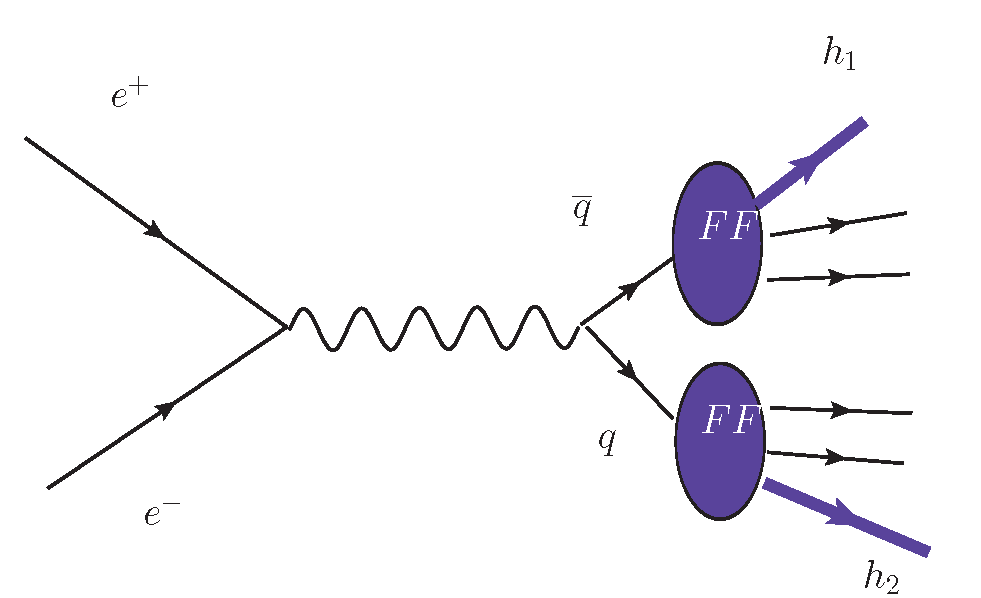
\includegraphics[width=0.8\textwidth,natwidth=610,natheight=642]{figure_theory/e+e-.png}
    \caption[Short caption]{The $e^+e^-$ annihilation process.}
    \label{fig:e+e-}
\end{figure}
The Collins mechanism describes the dependence of the transverse momentum of an unpolarized hadron on the transverse polarization of the parent quark. Here we define the transverse momentum with respect to the direction of the parent quark and call it $\boldsymbol{P}_{\bot}$, The transverse polarization of the transversely polarized quark is $\boldsymbol{S}_\perp$ and $\boldsymbol{k}$ is the momentum of the quark. The probability to find a hadron $h$ produced by a transversely polarized quark is\cite{ChargedPionResult,SSATrentoConvention}

\begin{equation}
D_{hq\uparrow}=D^q_1(z,P^2_{\bot})+H^{\bot q}_1(z,P^2_{\bot})\frac{(\hat{k}\times \boldsymbol{P}_{\bot})\cdot \boldsymbol{S}_{\perp}}{zM_h},
\label{eqn:FF1}
\end{equation}


In $e^+e^-\rightarrow q \bar q$  with unpolarized lepton lepton beams, we cannot measure a Collins effect in a single hemisphere, since we do not know the polarization of the parent quark. 
However, as shown in Fig.~\ref{fig:e+e-}, we can use the measurement of back-to-back hadrons, where the hadrons are detected in opposite hemispheres. In this case the correlation between the polarizations of the parent $q \bar q$ pair remains in the correlation of the Collins effects of $h_1$ and $h_2$~\cite{BoerThesis,ChargedPionResult2}. A naive picture is to think about the Collins effect as a left/right asymmetry. If we detect hadrons approximately perpendicular to the beam axis, we know that the parent quark was transversely polarized, but we don't know the direction. However, if we detect a hadron in the opposite hemisphere, we can measure the relative effect to that hadron which comes from quark with correlated polarization.

\subsubsection{Cross-section and Azimuthal Asymmetry in $e^+e^-$ Annihilation}

\begin{figure}[H]
  \centering     
  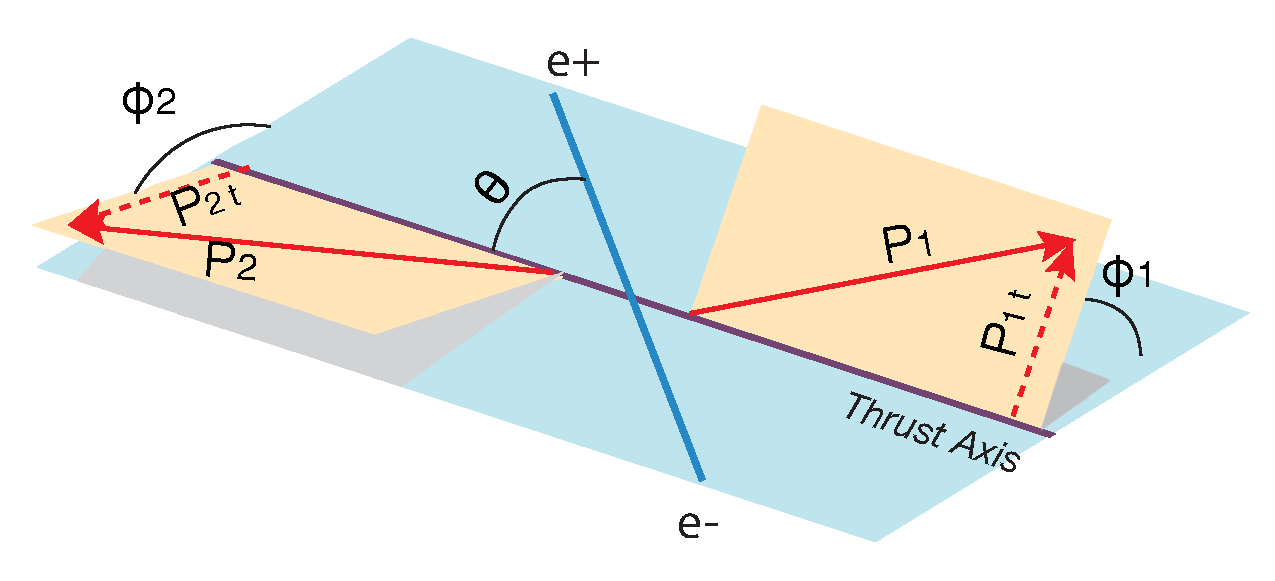
\includegraphics[width=.9\textwidth,natwidth=600,natheight=400]{figure_theory/e+e-_phi1phi2.pdf}
  \caption{Thrust reference frame.}
  \label{fig:phi1phi2frame}
\end{figure}

As discussed in~\cite{BoerThesis, Boer:2008fr}, the Collins effect in $e^+e^-$ can be measured in different frames which differ in the selection of the reference axis that is used to compute the azimuthal angles (For both frames the reference frame is the CMS). Either one chooses one of the hadrons ($h_1$) and measures the azimuthal angle of the other hadron around $h_1$, the so-called $\phi_0$ method, or one chooses the thrust axis of the event as the axis and measures the sum of the azimuthal angles $\phi_1$, $\phi_2$ of $h_1$ and $h_2$, respectively. This is sometimes called the $\phi_{12}$ method. We chose the later one. At leading order the thrust axis is connected to the unobserved $q \bar q$ axis, which connects this method to the naive description given earlier. It should be noted, that in previous measurements at Belle and BaBar, the thrust axis was corrected back to the $q \bar q$ axis from simulation. We do not do this for our analysis, since the matching to a leading order plus parton shower simulation is questionable, instead we will correct back to the true thrust axis to be defined later when we discuss the analysis.

Fig.~\ref{fig:phi1phi2frame} shows the frame that uses thrust axis as reference. The thrust axis~($\boldsymbol{\hat{n}}$) can be obtained by  maximizing:
\begin{equation}
\label{eq:thrust}
t=\sum_h\frac{|\boldsymbol{P_h\cdot\hat{n}}|}{|P_h|}.
\end{equation}
Here the summation runs over all stable final state particles. In experiment, not all final state particles can be collected thus the reconstructed thrust axis is not accurate. This effect will be discussed and corrected in subsection~\ref{sec:smearingcorrection}. 

In this reference frame, the differential cross-section is dependent on the fractional energies~($z_{1,2}$) and Collins angles~($\phi_{1,2}$) of hadron $h_{1,2}$ and expressed as~\cite{BoerThesis}:
\begin{equation}
\begin{aligned}
\frac{d\sigma(e^+e^-\rightarrow (\textrm{jet}+h_1)(\textrm{jet}+h_2)+X)}{d\Omega dz_1dz_2 d\boldsymbol{P}_{t1} d\boldsymbol{P}_{t2} d\phi_1d\phi_2}&\propto \\
\sum_{q,\bar{q}} \frac{3\alpha^2}{Q^2}\frac{e_q^2}{4}z^2_1z^2_2 \left\{ (1+\cos^2\theta)D_1^{q}(z_1,\boldsymbol{P}^2_{1\perp})\bar{D}_1^{\bar{q}}(z_2,\boldsymbol{P}^2_{2\perp})\right.\\  \left. +\sin^2\theta\cos(\phi_1+\phi_2)H_1^{\bot,q}(z_1,\boldsymbol{P}^2_{1\perp})\bar{H}_1^{\bot,\bar{q}}(z_2,\boldsymbol{P}^2_{2\perp})\right\},
\end{aligned}
\label{eqn:cross_subsection_ee}
\end{equation}
where the sum runs over all quark flavors accessible at the center-of-mass energy~\cite{BoerThesis}. In the leading order equation~\ref{eqn:cross_subsection_ee},  $\theta$ the angle between the colliding beam and the thrust axis.
The charge carried by each quark is written as $e_q$, $z_{1,2}$ and $\boldsymbol{P}_{1,2,\perp}$ are, as before, the fractional energies of the produced hadrons, $z_i\approx -\frac{2P_{i}\cdot q}{Q^2}=\frac{2*E_{h_i} }{\sqrt{s}}$,  and their transverse momentum with respect to $\boldsymbol{k}$. We call the observed transverse momentum of hadron $i$ with respect to the thrust axis $\boldsymbol{P}_{ti}$. In this work we extract the asymmetry using the leading order angular dependencies and substituting $\boldsymbol{P}_{ti}$ for $\boldsymbol{P}_{i\perp}$ and the thrust axis for the $q-\bar{q}$ axis. 

Equation.~\ref{eqn:cross_subsection_ee} can be written more compactly as:
\begin{equation}
d\sigma \sim A D_1^q \bar{D}_1^{\bar{q}}+B\cos(\phi_1+\phi_2)H^{\bot q}_{1}\bar{H}^{\bot \bar{q} }_{1}.
\label{eqn:FF2}
\end{equation}
\noindent where in Eq.~\eqref{eqn:FF2}, $A(y)=(\frac{1}{2}-y+y^2)$ and $B(y)=y(1-y)$. In the CMS, $A$ and $B$ can be described as $A(y)=\frac{1}{4}(1+\cos^2\theta)$ and $B(y)=\frac{1}{4}\sin^2\theta$. 

%Collins Fragmentation Function appears in the first order transverse moment as~\cite{AsyInPolarizedHadronProductionInEE}:
%\begin{equation}
%H_1^{\bot(1)}=z^2\int d^2 \boldsymbol{k}_T \frac{\boldsymbol{k}_T^2}{2M^2} H_1^{\bot}(z,z^2\boldsymbol{k}_T^2)
%\label{eqn:firstmomet}
%\end{equation}
%\noindent where $H^{\bot q}_1(z,P^2_{h\bot})$ is the Collins FF. Similarly with subsection~\ref{sec:SIDIScrosssubsection}, $z$ is defined as the fractional energy of the hadron $z\approx -\frac{2P_h\cdot q}{Q^2}=\frac{2*E_h}{\sqrt{S}}$. 
%The last item in Eq.~\eqref{eqn:FF1} is dependent on the quark spin direction and hence the transverse distribution function will lead to an asymmetric azimuthal angle distribution as shown in Eq.~\eqref{eqn:tssa}.   

\subsection{Observable}
\label{sec:observable}
A hadron pair is composed of hadrons $h_1$, $h_2$ from different hemispheres (back-to-back), which means for their respective three momenta $\boldsymbol{P}_{i}$:
\begin{equation}
(\boldsymbol{P}_{1} \cdot \hat{n})(\boldsymbol{P}_{2}\cdot \hat{n}) < 0 .
\end{equation}
If the two hadrons in different hemispheres are measured simultaneously, the Collins asymmetry will be proportional to $\cos(\phi_1+\phi_2)$. The angles $\phi_1$ and $\phi_2$ are shown in Fig.~\ref{fig:phi1phi2frame} and can be calculated using
\begin{equation}
%\phi_i=\frac{\hat{\boldsymbol{n}}}{|\hat{\boldsymbol{n}|}}\cdot(\frac{\hat{\boldsymbol{z}}\times\hat{\boldsymbol{n}}}{|\hat{\boldsymbol{z}}||\hat{\boldsymbol{n}}|}\times\frac{\hat{\boldsymbol{n}}\times\hat{\boldsymbol{P}_{h,i}}}{|\hat{\boldsymbol{n}}||\hat{\boldsymbol{P}_{h,i}}|})\arccos(\frac{\hat{\boldsymbol{z}}\times\hat{\boldsymbol{n}}}{|\hat{\boldsymbol{z}}||\hat{\boldsymbol{n}}|}\times\frac{\hat{\boldsymbol{n}}\times\hat{\boldsymbol{P}_{h,i}}}{|\hat{\boldsymbol{n}}||\hat{\boldsymbol{P}_{h,i}}|}),
\phi_i=sgn[\hat{\boldsymbol{n}}\cdot \{ (\boldsymbol{z}\times\hat{\boldsymbol{n}})\times(\hat{\boldsymbol{n}}\times{\boldsymbol{P}_{i}})\}]\times \arccos(\frac{\hat{\boldsymbol{z}}\times\hat{\boldsymbol{n}}}{|\hat{\boldsymbol{z}}\times\hat{\boldsymbol{n}}|}\times\frac{\hat{\boldsymbol{n}}\times{\boldsymbol{P}_{i}}}{|\hat{\boldsymbol{n}}\times{\boldsymbol{P}_{i}}|}),
\label{eqn:collinsangledefine2}
\end{equation}
here $i$ stands for the hadron from first or second hemisphere and $\boldsymbol{z}$ is the unit vector along the beam direction.

The Collins angle of a hadron pair is $\phi_{12} \equiv \phi_1+\phi_2$. The di-hadron yield $N_{12}=N_{12}(\phi_1+\phi_2)$ divided by the average yield gives the normalized rate $R_{12}=\nicefrac{N_{12}}{\langle  N_{12}\rangle}$. Considering the $\cos(\phi_1+\phi_2)$ modulation, $R_{12}$ can be parameterized as $R_{12}=a_{12}(\theta,z_1,z_2, \boldsymbol{P}^2_{h1\bot},\boldsymbol{P}^2_{2\bot})\cos(\phi_1+\phi_2)+b_{12}$ with the azimuthal asymmetry
\begin{equation}
a_{12}(\theta,z_1,z_2, \boldsymbol{P}^2_{t1},\boldsymbol{P}^2_{t2})=\frac{\sin^2\theta}{1+\cos^2\theta}
\frac{\sum\limits_{q}e^2_qH^{\bot q}_1(z_1,\boldsymbol{P}^2_{t1})\bar{H}^{\bot q}_1(z_2,\boldsymbol{P}^2_{t2})}{\sum\limits_{q}e^2_qD^q_1(z_1,\boldsymbol{P}^2_{t1})\bar{D}^{\bar{q}}_1(z_2,\boldsymbol{P}^2_{t2})}.
\end{equation} 
Here $b_{12}$ is the normalized yield which should be consistent with 1.
Note that in the equation for $a_{12}$ above, we kept the full dependence of the asymmetry $a_{12}$ on the $z_i$ and $ \boldsymbol{P}^2_{ti}$. In the measurements presented later in the note, we keep at most two variables differential, the other ones are integrated out (There is no convolution over the transverse momenta since this is the thrust method, not the $\phi_0$ method).
As will be discussed later (see subsection~\ref{sec:dataselection}), the azimuthal distribution can be strongly distorted due to acceptance effects. Furthermore, initial-state radiation (ISR) and gluon radiation introduce cosine modulations similar to the ones arising from the Collins effect. To remedy those effects the double ratio (DR) method, in which we calculate the ratio of normalized distribution between certain different kinds of hadron pairs, can be used as the effects are assumed to be charge independent and thus largely cancel during the ratio calculation~\cite{ChargedPionResult,CollinsInSIDISandEE}.  For example, in the charged pion analysis, the double ratio was designed to be the ratio of unlike sign pairs ($\pi^+\pi^-$) to like sign pairs ($\pi^+\pi^+$ and $\pi^-\pi^-$).


In this note, double ratios for neutral mesons are designated as:
\begin{equation}
\label{eqn:FF6}
\begin{aligned}
A_{12}^{\pi^0}=\frac{A^{0\pm}_{12}}{A^L_{12}}=\frac{\pi^0\pi^++\pi^0\pi^-}{\pi^+\pi^++\pi^-\pi^-}\\
A_{12}^{\eta}=\frac{A^{\eta\pm}_{12}}{A^L_{12}}=\frac{\eta\pi^++\eta\pi^-}{\pi^+\pi^++\pi^-\pi^-}.
\end{aligned}
\end{equation}
For charged pions we can consider asymmetries of likesign pairs (L), unlikesign pairs (U) or pairs that are integrated over both charges (C).
With these we can construct three more double ratios:

\begin{equation}
\label{eqn:FF7}
\begin{aligned}
A_{12}^{UL}=\frac{A^{U}_{12}}{A^L_{12}}=\frac{\pi^+\pi^-+\pi^-\pi^+}{\pi^+\pi^++\pi^-\pi^-}\\
A_{12}^{UC}=\frac{A^{U}_{12}}{A^C_{12}}=\frac{\pi^+\pi^-+\pi^-\pi^+}{\pi^+\pi^++\pi^-\pi^-+\pi^+\pi^-+\pi^-\pi^+}\\
A_{12}^{CL}=\frac{A^{U}_{12}}{A^C_{12}}=\frac{\pi^+\pi^++\pi^-\pi^-+\pi^+\pi^-+\pi^-\pi^+}{\pi^+\pi^++\pi^-\pi^-}.
\end{aligned}
\end{equation}


The asymmetry $A^C$ is thought to be related to the asymmetries involving $\pi^0$'s, therefore the double ratio $A_{12}^{CL}$ should be equal to $A_{12}^{\pi^0}$~\cite{Efremov:2006qm}, 
which we will test with the experimental data.
%For the Collins effect, the Collins FF can be separated into favored and unfavored parts according to which flavor goes into the hadron where charge-conjugation and isospin symmetry arguments have been used~\cite{CollinsInSIDISandEE}:


Fragmentation functions are often categorized into favored and disfavored ones, depending on whether or not the fragmenting-quark flavor is part of the valence structure of the hadron formed. For charged pions, employing charge-symmetry and isospin asymmetry, FFs are 
\begin{equation}
\begin{aligned}
D^{fav}=D^{u/{\pi^+}}=D^{d/{\pi^-}}=D^{\bar{u}/{\pi^-}}=D^{\bar{d}/{\pi^+}}\\
D^{dis}=D^{u/{\pi^-}}=D^{d/{\pi^+}}=D^{\bar{u}/{\pi^+}}=D^{\bar{d}/{\pi^-}}.
\label{eqn:FF4}
\end{aligned}
\end{equation}
The fragmentation functions of $\pi^0$ consist of both favored and disfavored FFs~\cite{FoundationsofpQCD,Efremov:2006qm},
\begin{equation}
\begin{aligned}
D^{u/{\pi^0}}=D^{\bar{u}/{\pi^0}}=D^{d/{\pi^0}}=D^{\bar{d}/{\pi^0}}=\frac{1}{2}(D^{dis}+D^{fav}).
\label{eqn:FF4pi0}
\end{aligned}
\end{equation}
Besides light quarks, we also consider the contribution of strange quarks.
% A common assumption is that the probability for strange-quark fragments into charged pions is the same as the light-quark disfavored ones, as it also requires generating the two valence quarks forming the pion, thus
A common assumption is that the probability for strange-quark fragmentation is the same for all pion states, thus
\begin{equation}
D^{dis}_{s\rightarrow\pi}=D^{s/{\pi^-}}=D^{s/{\pi^+}}=D^{s/{\pi^0}}.
\end{equation}

Asymmetries after applying the double ratio, for instance, like sign pairs $A^L_{12}$ and $\pi^0\pi^{\pm}$ pairs $A^{0\pm}_{12}$, can be expressed in terms of various FFs~\cite{Efremov:2006qm}:

\begin{multline}
A_{12}^{\pi^0}=\frac{A^{0\pm}_{12}}{A^L_{12}}=1+\cos(\phi_1+\phi_2)\frac{\sin^2(\theta)}{1+\cos^2(\theta)} \\
\times\bigg\{\frac{5(H^{\bot,fav}_1+H^{\bot,dis}_1)(H^{\bot,dis}_1+H^{\bot,fav}_1)+4H^{\bot,dis}_{1,s\rightarrow\pi}H^{\bot,dis}_{1,s\rightarrow\pi}}{5(D^{\bot,fav}_1+D^{\bot,dis}_1)(D^{\bot,dis}_1+D^{\bot,fav}_1)+4D^{dis}_{1,s\rightarrow\pi}D^{dis}_{1,s\rightarrow\pi})}\\
-\frac{5H^{\bot,fav}_1H^{\bot,dis}_1+5H^{\bot,dis}_1H^{\bot,fav}_1+2H^{\bot,dis}_{1,s\rightarrow\pi}H^{\bot,dis}_{1,s\rightarrow\pi}}{5D^{\bot,fav}_1D^{\bot,dis}_1+5D^{\bot,dis}_1D^{\bot,fav}_1+2D^{dis}_{1,s\rightarrow\pi}D^{dis}_{1,s\rightarrow\pi}} \bigg\}.
\label{eqn:FF5}
\end{multline}
%Due to the differing valence structure of the $\eta$, the FFs composition the relations above~\ref{eqn:FF5} read differently:

To study the FFs expression of $\eta$, due to the different valence structure with $\pi^0$, we need to reconsider the cases with strange-quark fragments into $\eta$. 
\begin{equation}
\begin{aligned}
D^{u/{\eta}}=D^{d/{\eta}}=D^{\bar{u}/{\eta}}=D^{\bar{d}/{\eta}}=D^{s/{\eta}}=D^{\bar{s}/{\eta}}=\frac{1}{2}\left(D^{fav_\eta}+D^{dis_\eta}\right).
\label{eqn:FFetaquark}
\end{aligned}
\end{equation}

Neglecting symmetry breaking due to strangeness suppression, the strange-quark FFs can be related to the non-strange ones:
\begin{equation}
\begin{aligned}
D^{s/{\eta}}=D^{\bar{s}/{\eta}}=\frac{1}{2}\left(D^{fav_\eta}+D^{dis_\eta}\right).`
\end{aligned}
\end{equation}
However, here we do not use this relation. Using~\ref{eqn:FFetaquark} results in the following expression for the double ratio:
\begin{multline}
A_{12}^{\eta}=\frac{A^{\eta\pm}_{12}}{A^L_{12}}=1+\cos(\phi_1+\phi_2)\frac{\sin^2(\theta)}{1+\cos^2(\theta)} \\
\times\bigg\{\frac{5(H^{\bot,fav_\eta}_1+H^{\bot,dis_\eta}_1)(H^{\bot,dis}_1+H^{\bot,fav}_1)+2(H^{\bot,fav}_{1,s\rightarrow\eta}+H^{\bot,dis}_{1,s\rightarrow\eta})H^{\bot,dis}_{1,s\rightarrow\pi}}{5(D^{\bot,fav_\eta}_1+D^{\bot,dis_\eta}_1)(D^{\bot,dis}_1+D^{\bot,fav}_1)+2(D^{dis}_{1,s\rightarrow\eta}+D^{dis}_{1,s\rightarrow\eta})D^{dis}_{1,s\rightarrow\pi})}\\
-\frac{5H^{\bot,fav}_1H^{\bot,dis}_1+5H^{\bot,dis}_1H^{\bot,fav}_1+2H^{\bot,dis}_{1,s\rightarrow\pi}H^{\bot,dis}_{1,s\rightarrow\pi}}{5D^{\bot,fav}_1D^{\bot,dis}_1+5D^{\bot,dis}_1D^{\bot,fav}_1+2D^{dis}_{1,s\rightarrow\pi}D^{dis}_{1,s\rightarrow\pi}} \bigg\}.
\label{eqn:FF5eta}
\end{multline}

The parameterization $A_{12}*\cos(\phi_1+\phi_2)$ is fitted to the final double ratio distribution, where the amplitude $A_{12}$ is the azimuthal asymmetry that is measured in this note. 

\section{Data Selection and Meson Reconstruction}
\label{sec:dataselection}
This section outlines the general criteria used to reconstruct neutral mesons from $\gamma$ pairs as well as the selection criteria that are used to select good hadronic events in which $(udsc)$ quarks fragment into back-to-back jets. After a short discussion of the relevant parts of the Belle detector, we introduce the event selection criteria in sub-section~\ref{sec:eventselection}. Our cuts are based on similar analysis of fragmentation functions documented in Belle notes $\#805$, $\#878$, $\#902$ and $\#1346$. 
Subsequently we introduce the binning used to extract the Collins asymmetries in sub-section~\ref{sec:kinematicbins}.
Finally, sub-sections~\ref{sec:fiducialcut} and~\ref{sec:neutralmesonreconstruction} introduce the fiducial cuts for the $\gamma$ selection and reconstruction of the $\pi^0$ and $\eta$ mesons.
The Monte Carlo used in this note was generated by EvtGen or QQ98 generators and the simulation of Belle detector is based on GEANT3 package \cite{DetectorSimulation}. 

\subsection{Belle Detector Introduction}
The Belle detector comprises the following main parts: Beam pipe, Extreme Forward Calorimeter~(EFC), Silicon Vertex Detector~(SVD), Central Drift Chamber~(CDC), Aerogel Cherenkov Counter~(ACC), Time of Flight Counter (TOF), Electromagnetic Calorimeter (EMCAL), $K_L$ and muon detection system~(KLM).
 This analysis is focused on identified tracks and neutral mesons. Thus the most important detector components are the CDC,  EMCAL, TOF, ACC and KLM.
 The CDC is used to reconstruct the track of charged particles and precisely measure the momentum of charged particles.  The TOF measures the flight time of particles and separates particles with different masses. It is mainly efficient for low energy particles. The ACC separates kaons and pions with momentum from $1.2$~GeV$/c$ to $3.5$~GeV$/c$. The purpose of EMCAL is to efficiently detect photons and provide good resolution of energy and position. Finally, the KLM consists of tracking chambers sandwiched in layers of steel and it can be used to identify muons by their penetration depth. In the Belle data summary tables, the combined information of the PID detectors is presented as a set of likelihoods for a given particle to be of species $i$ vs species $j$. Our particle identification criteria outlined in the next section are thus in terms of these likelihoods. 

\subsection{Event Selection}
\label{sec:eventselection}
The constraints used for event selection are:
\begin{itemize}
\item To reduce contributions from $\tau$ production we require a minimum visible energy of $7$~GeV.  This excludes events where an undetected neutrino carries away a signficant fraction of the total energy.
\item Vertex position is restricted to the range:
\begin{center}
$d_{vertex}<2$~cm   \\
$\lvert z_{vertex}\rvert < 4$~cm
\end{center}
\item Thrust $t>0.8$.
\item PID uses the following cuts on the particle likelihoods:
\begin{itemize}
  \item electron: $\mathcal{L}(e)>0.85$
  \item muon: $\mathcal{L}(\mu)>0.85$
 % \item Kaon: $\nicefrac{\mathcal{L}(p)}{\mathcal{L}(\mathcal{K})}>0.8$
  \item kaon: $\nicefrac{\mathcal{L}(\mathcal{K})}{\mathcal{L}(\pi)}>0.6$
  \item proton: $\nicefrac{\mathcal{L}(\mathcal{P})}{\mathcal{L}(K)}>0.8$
  \item Pion: $\nicefrac{\mathcal{L}(\mathcal{K})}{\mathcal{L}(\pi)}<0.3$
\end{itemize}
\end{itemize}
After applying the PID selection, the efficiency of identified charged pions is around $96.9\%$.

\subsection{Kinematic Bins}
\label{sec:kinematicbins}
As described in the previous section and e.g. expressed in Eq.~\eqref{eqn:FF1}, the Collins asymmetries depend on $z$ and the transverse momentum $P_t$\footnote{In this analysis, we use $\perp$ to represent the transverse momentum to the real $q\bar{q}$ axis. And the subscript $t$ denotes the transverse momentum to thrust axis.}.  
Fig.~\ref{fig:zptdistri} shows the distribution of $z$ and $P_t$ of the neutral and charged pions as well as $\eta$ mesons used in this analysis. Since we use ratios of different particle combinations to cancel detector effects and we often integrate over one of the kinematic dependencies, it minimizes our systematic effects if the kinematic distributions are similar between the different particle species. We achieve this by introducing fiducial cuts which are described in sec.~\ref{sec:fiducialcut}. Figure~\ref{fig:zptdistri} shows the distributions after the application of these cuts.
\begin{figure}[H]
  \centering     
  \subfigure[$z$ distribution of mesons]{\label{fig:pi0z}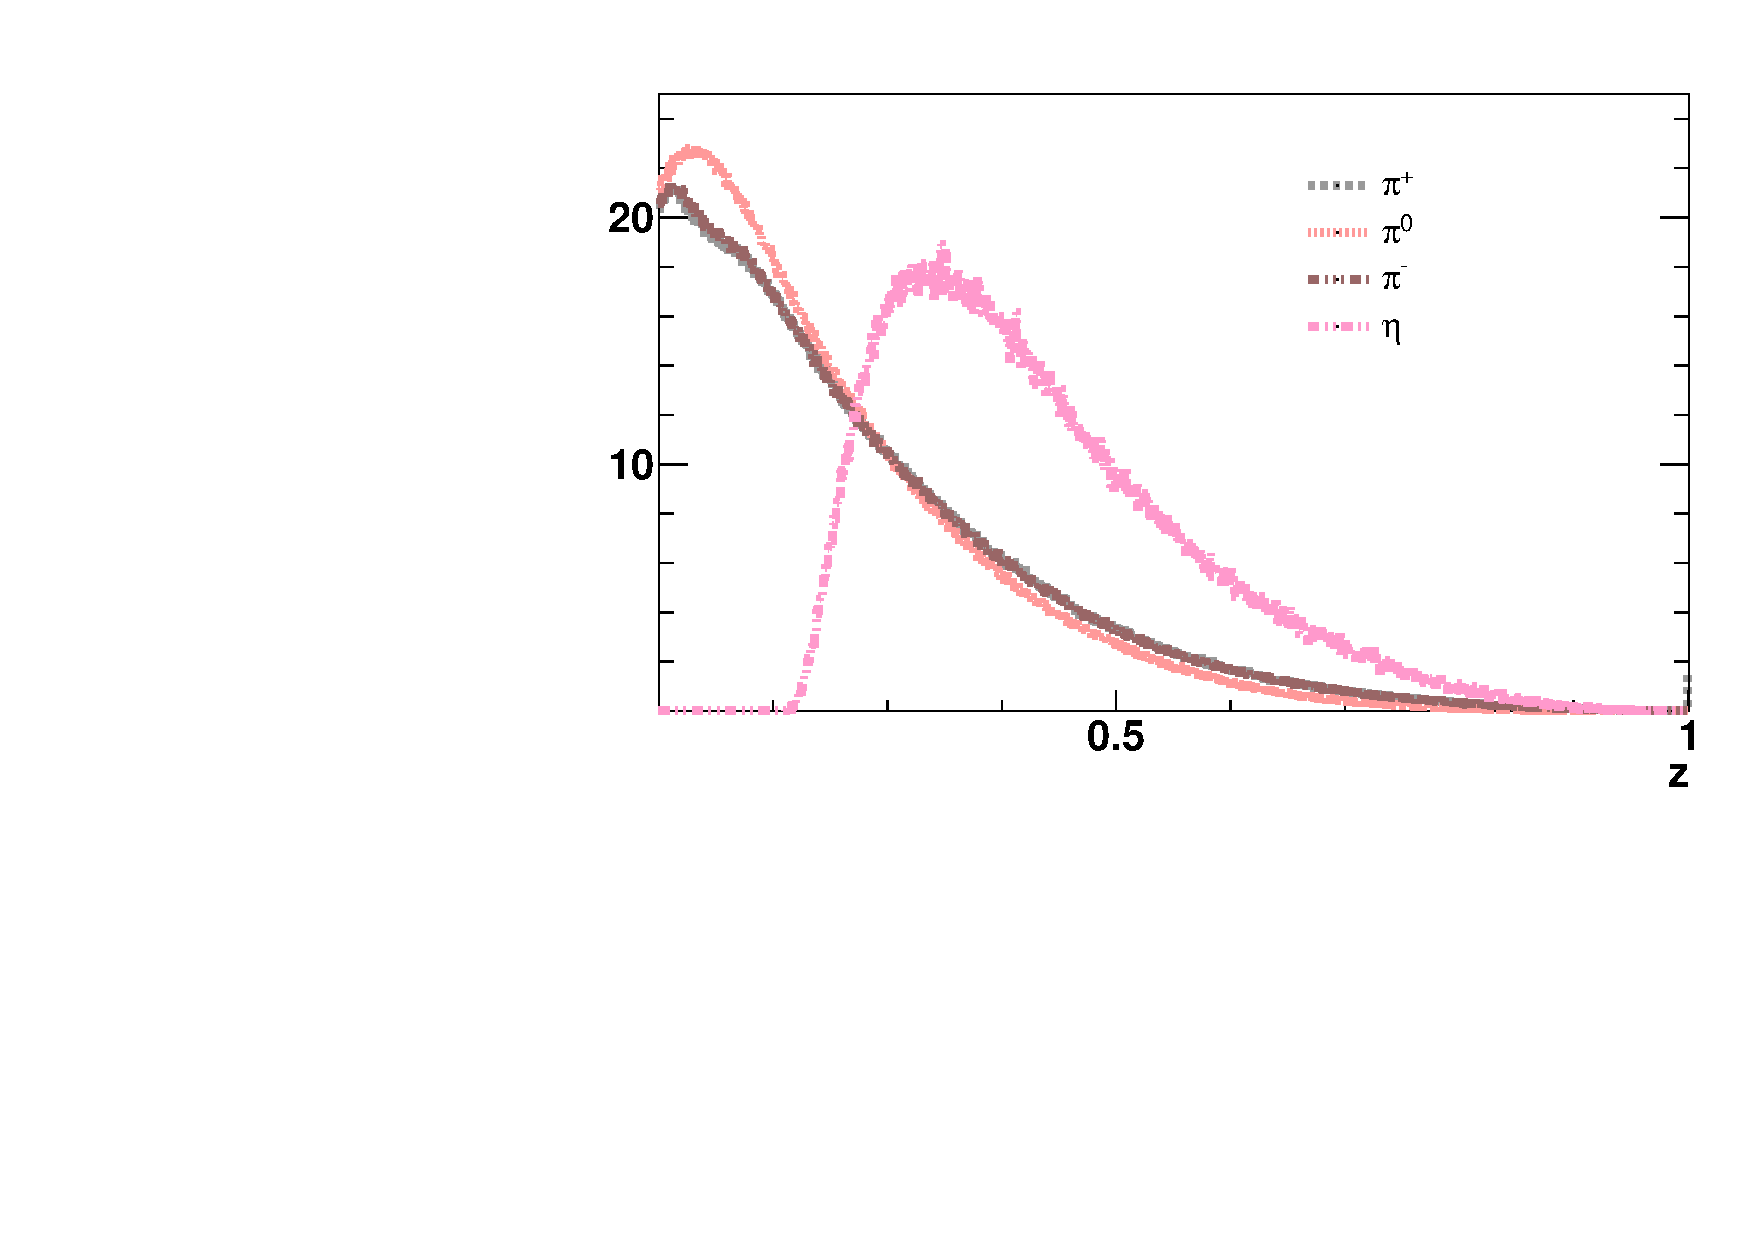
\includegraphics[width=.48\textwidth,natwidth=600,natheight=400]{figure_dataselection/Z_distri.pdf}}
  \subfigure[$P_t$ distribution of mesons]{\label{fig:pi0pt}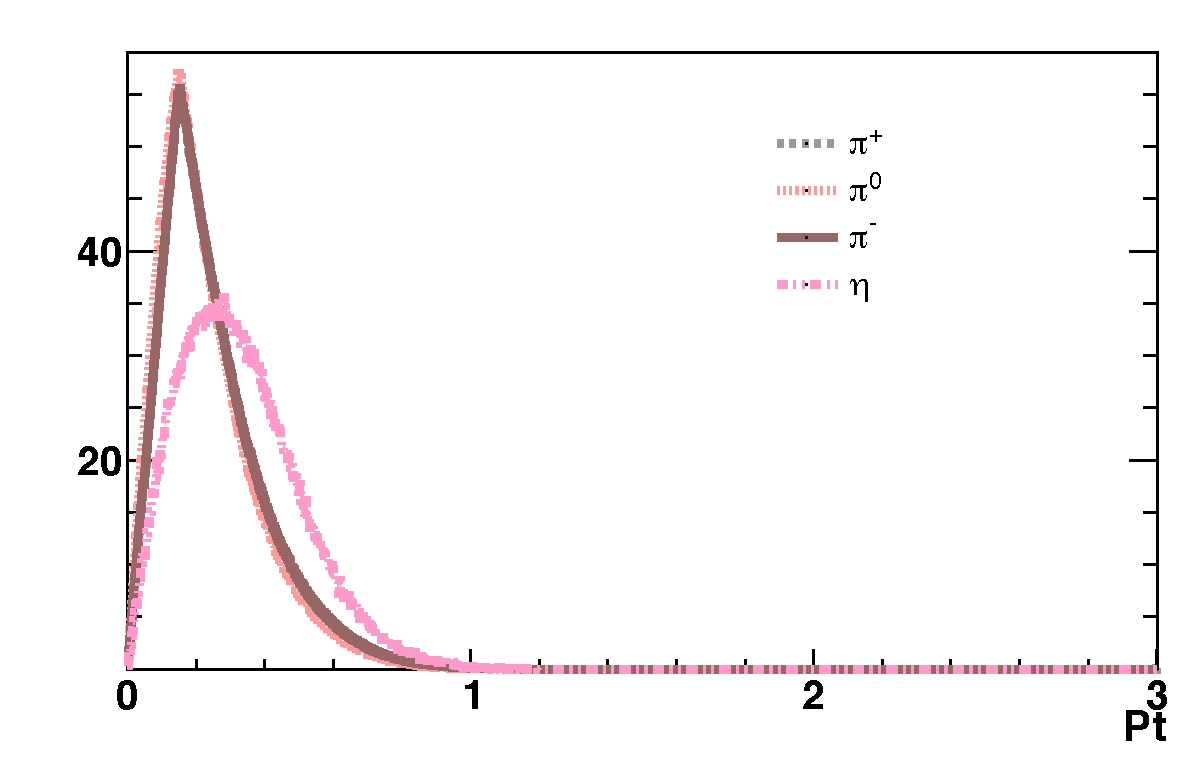
\includegraphics[width=.48\textwidth,natwidth=600,natheight=400]{figure_dataselection/Pt_distri.pdf}}
  \caption{Normalized distribution of kinematic distributions with all event selection, fiducial requirements and the neutral meson reconstruction criteria (see section~\ref{sec:neutralmesonreconstruction}) applied. Left plot is the $z$ distribution of experimental data. The right plot is $P_t$ distribution. The $z$ distribution of the $\eta$ distribution is shifted with respect to the pions due to the higher mass and higher photon energy cut of the $\eta$. In ratios involving the $\eta$ we can remedy this by applying an appropriate $z$ cut on the pions as well.}
  \label{fig:zptdistri}
\end{figure}

Two kinds of kinematic bins have been studied. In order to study both kinematic dependences the first hadron of the hadron pair is either binned in $z$ or $P_t$ according to the bin boundaries given in Tables~\ref{tab:whatissinglez} and~\ref{tab:whatissinglept}. For the neutral/charged mixed hadron pairs, we take the neutral hadron as the first hadron in a hadron pair and the kinematics of first hadron will be labeled with index $1$. While for charged hadron pairs we randomly pick one hadron as the first one. For the binnings that depend solely on $z$ or $P_t$, the bin number is determined by the first hadron and the dependence on $z_2$ and $P_{t2}$ is integrated out. 
\begin{table}[H]\small
\centering
\begin{tabular}{|l|l|l|l|l|l|l|l|l|}
\hline
$z_1$ bins & 0 &  1 & 2 & 3 & 4 & 5 & 6  \\ \hline
 $z_1$  & {\color{red}0.1$\textup{--}$0.2} & 0.2$\textup{--}$0.3 & 0.3$\textup{--}$0.4 & 0.4$\textup{--}$0.5 & 0.5$\textup{--}$0.6 & 0.6$\textup{--}$0.7 & 0.7$\textup{--}$1  \\ \hline
\end{tabular}
\caption{Bin boundaries for the first-hadron's fractional energy $z_1$ used in the analysis of one-dimensional dependences of the Collins effect. The first $z$ bin, indicated in red, will only be used in the $(z_1,z_2)$  binning. See text for more details.}
\label{tab:whatissinglez}
\end{table}
The Collins effect of the lowest $z$ bin is expected to be small since on average low $z$ particles are produced after multiple string breaks in the fragmentation process, losing spin information in the process. Additionally we show later in section~\ref{sec:fiducialcut}, that remaining detector effects are strongest for this $z$ bin. Therefore we drop this bin by introducing a cut of $z>0.2$ for all binnings where we integrate over $z$. For these binnings, the lowest $z$ bin with its high statistics would just serve to dilute our measurement. We keep the bin for the $(z_1,z_2)$ binning.


\begin{table}[H]\small
\centering
\begin{tabular}{|l|l|l|l|l|l|l|l|l|l|l|l|l|l|l|l|l|l|}
\hline
 $P_{t1}$ bins & 0 &  1 & 2 & 3   \\ \hline
 $P_{t1}$ (GeV)  & 0$\textup{--}$0.15& 0.15$\textup{--}$0.3 & 0.3$\textup{--}$0.5 & 0.5$\textup{--}$3  \\ \hline
\end{tabular}
\caption{Bin boundaries for the first-hadron's transverse momentum $P_{t1}$ used in the analysis of one-dimensional dependences of the Collins effect}
\label{tab:whatissinglept}
\end{table}

In addition to studying the dependence of the asymmetry on the kinematics of the first hadron (integrating out the dependence on the second hadron),  we also study the dependence of the asymmetry on both hadrons. 
In previous charged pion analyses, a reduced binning  as shown in Fig.~\ref{fig:comz_mark} was used. Here additional bin combinations are eliminated that are symmetric under the interchange of the particle order.
\begin{figure}[H]
\centering
\begin{minipage}{.5\textwidth}
  \centering
  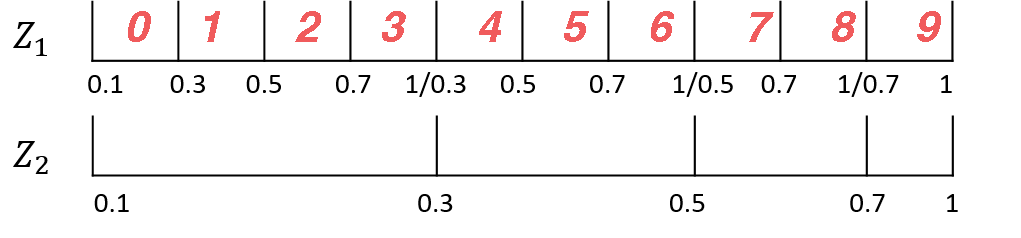
\includegraphics[width=0.95\textwidth,natwidth=610,natheight=642]{figure_dataselection/zbin.pdf}
  \captionof{figure}{$(z_1,z_2)$ bins used in pervious charged pion analysis.}
  \label{fig:comz_mark}
\end{minipage}%
%\begin{minipage}{.5\textwidth}
 % \centering
  %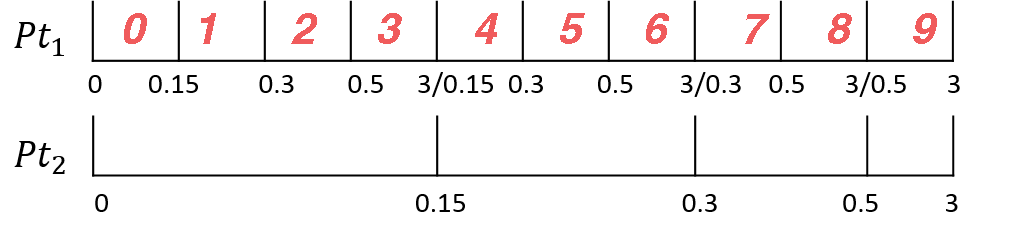
\includegraphics[width=0.95\textwidth,natwidth=610,natheight=642]{figure_dataselection/ptbin.pdf}
 % \captionof{figure}{$(P_{t1},P_{t2})$ bins }
  %\label{fig:compt_mark}
%\end{minipage}
\end{figure}
However, for the present analysis we consider combinations where the hadrons have different flavor content or iso-spin. 
Therefore we use the non-reduced  binning shown in Fig.~\ref{fig:binnings}. To further investigate the dependence of the asymmetry on $z$ and $P_t$ simultaneously, we also used a binning differential in $z$ and $P_t$ of the first hadron as indicated in Fig.~\ref{fig:zptbin}.   
\begin{figure}[H]
\captionsetup[subfloat]{farskip=2pt,captionskip=1pt}
\centering
\subfigure[$(z_1,z_2)$ bins]{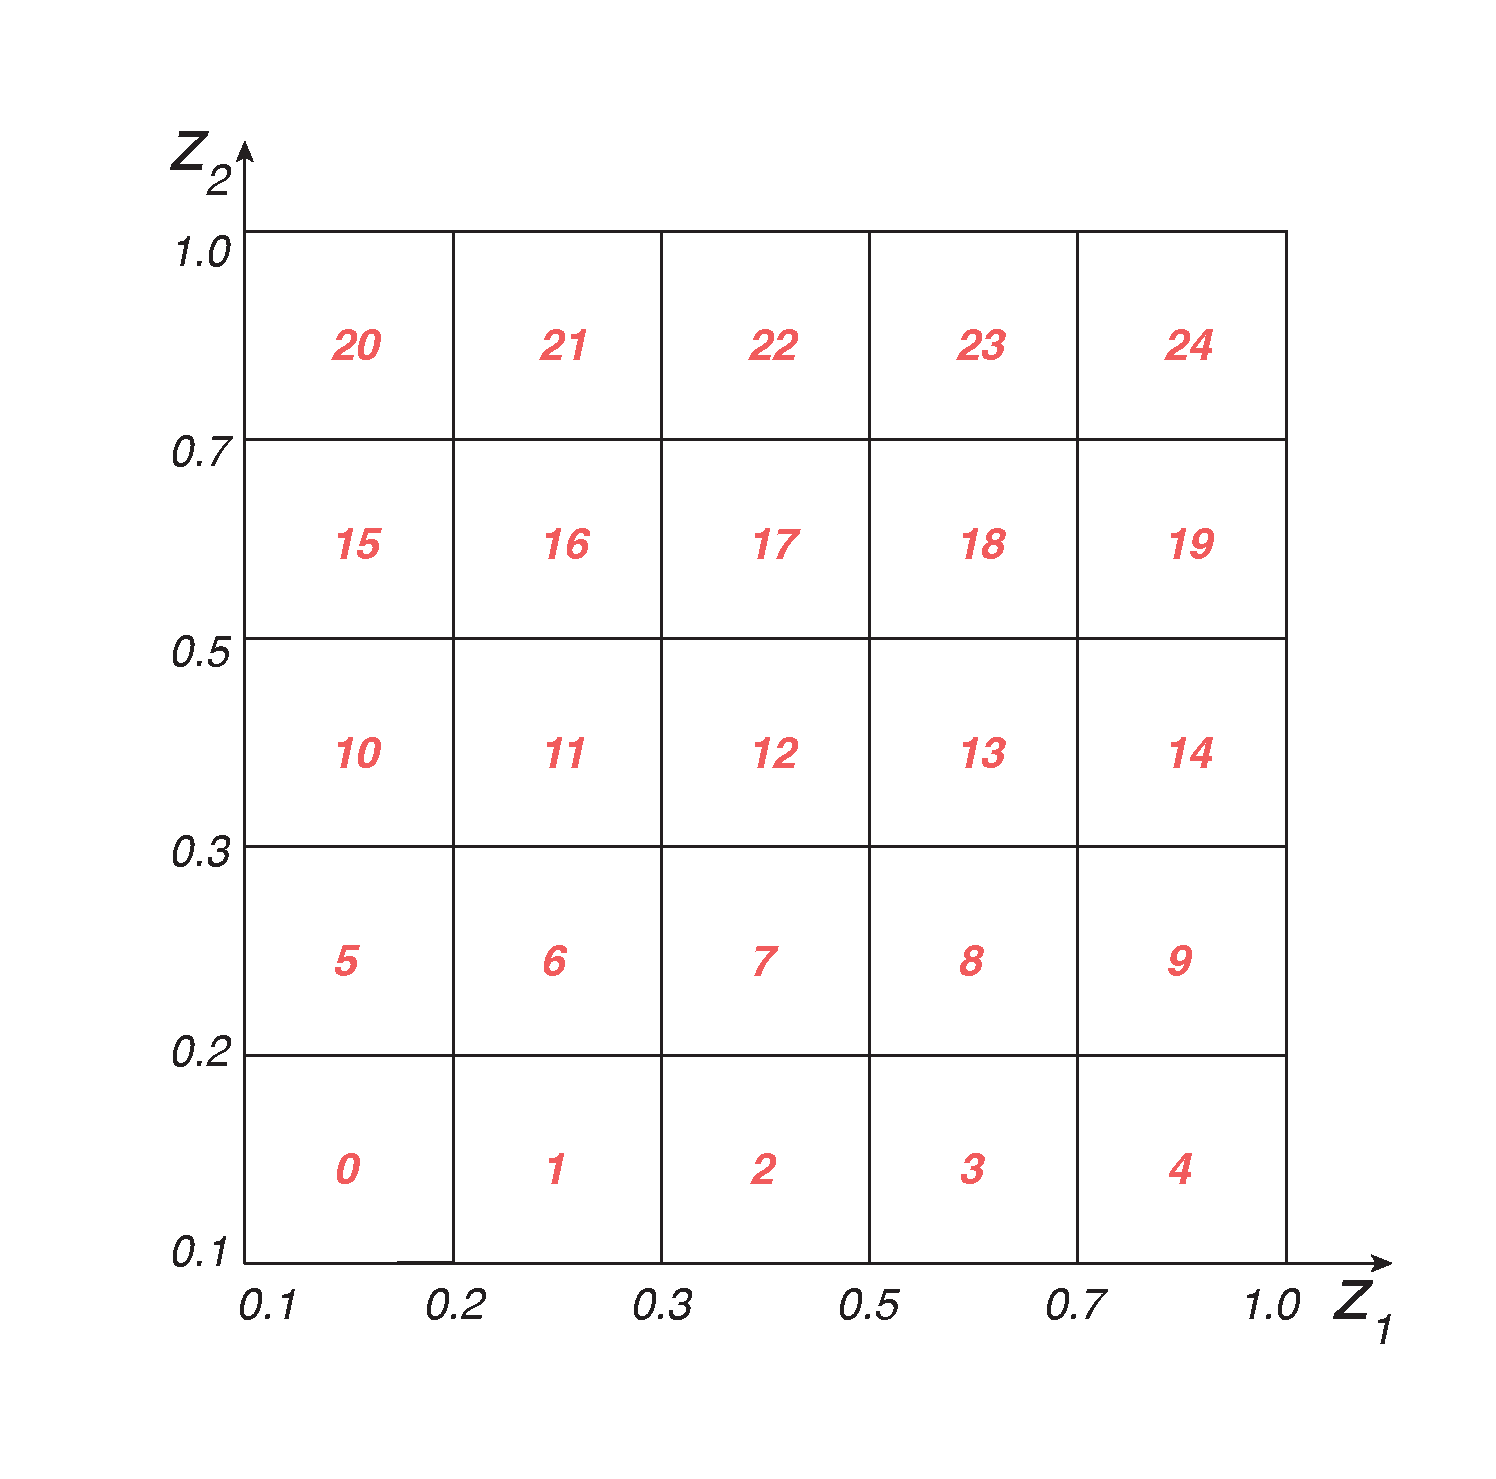
\includegraphics[width=.48\textwidth,natwidth=250,natheight=100]{figure_dataselection/comzbin.pdf}\label{fig:z1z2binning}}
\subfigure[$(P_{t1},P_{t2})$ bins]{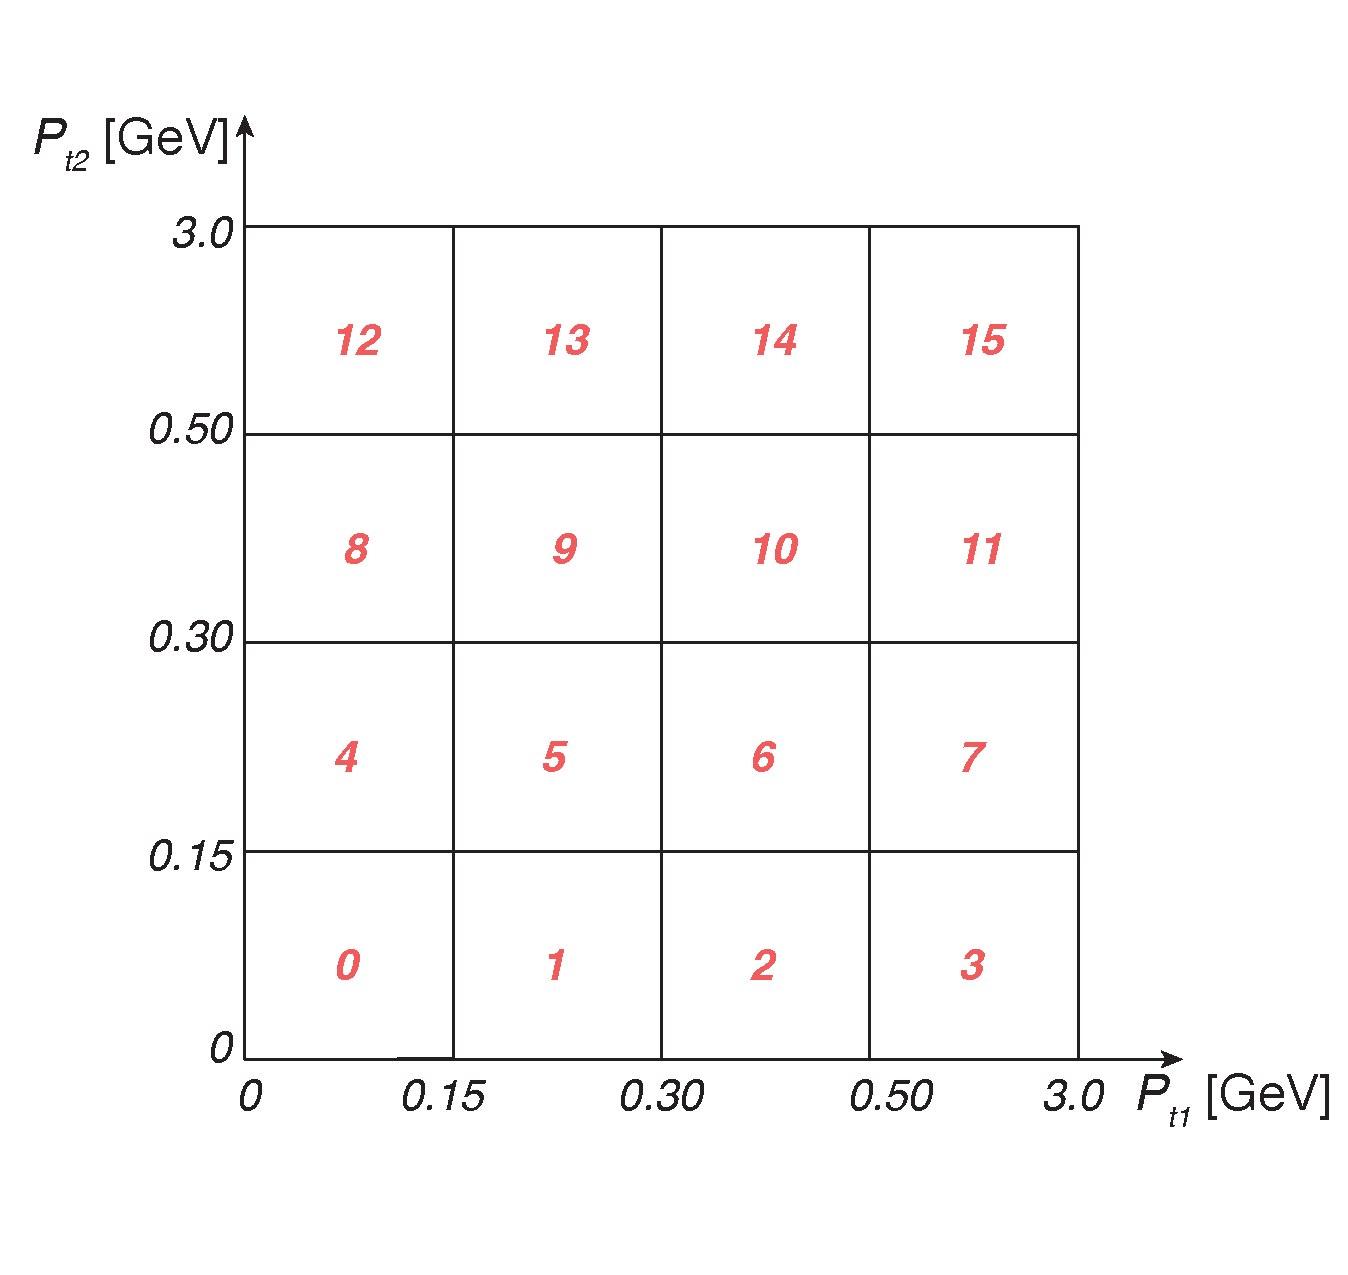
\includegraphics[width=.48\textwidth,natwidth=250,natheight=100]{figure_dataselection/comptbin.pdf}\label{fig:pt1pt2binning}}
\caption{Bin boundaries and numbering for the (hadron1, hadron2) bins. The index of the bin is indicated as a red number	.}
\label{fig:binnings}
\end{figure}

\begin{figure}[H]
    \centering
    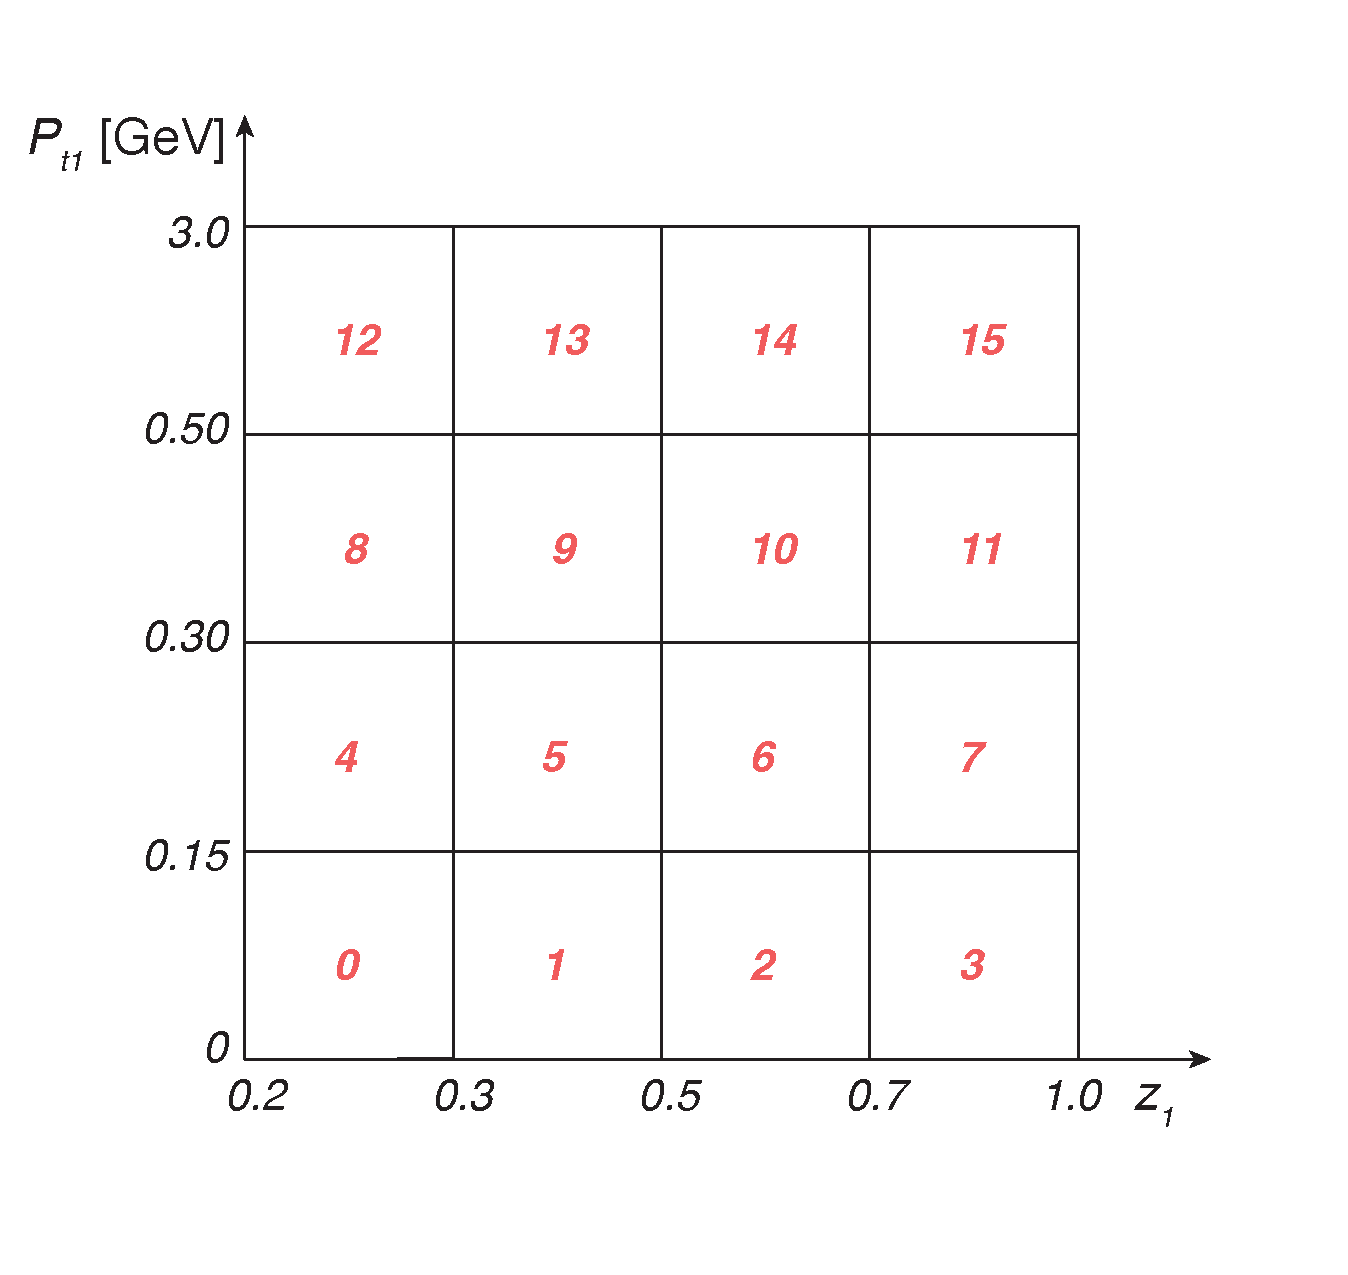
\includegraphics[width=0.6\textwidth,natwidth=250,natheight=100]{figure_dataselection/zptbin.pdf}
    \caption{Bin boundaries and numbering for the 2d binning of the neutral-meson kinematics $z$ and $P_t$.}
    \label{fig:zptbin}
\end{figure}



%%%%%%%%%%%%%%%%%%%%%%%%%%%%%%%%%%%%%%%%%%%


\subsection{Fiducial and Energy Constraints for Hadron Selection}
\label{sec:fidAndEnergyCuts}
In the following we discuss the fiducial cuts and photon energy constraints on the hadron selection. The fiducial cuts are defined in terms of an opening angle of the hadron or photon with respect to the
thrust axis. This is discussed in detail in Sec.~\ref{sec:fiducialcut} below. We use a grid search on the fiducial cuts and the photon energy to find cuts that optimize the Figure-Of-Merit (FOM) $\nicefrac{S}{\sqrt{N}}$ . This initial set of fiducial cuts is then refined to equalize kinematic distributions between the different hadron species.

\subsubsection{\texorpdfstring{Energy Constraint for $\gamma$ and mesons}{Energy Constraint for gamma and mesons}}

The $\gamma$ energy threshold and energy asymmetry are studied to reduce the background contribution. A higher threshold leads to more pure data at the expense of yield loss. Similarly, a tighter energy asymmetry requirement should also improve the signal purity while potentially reducing the yield. However, it was found that an asymmetry cut in addition to the energy threshold cut, does not improve the FOM significantly and we did not apply an asymmetry cut.
%as shown in Fig~\ref{fig:photon_asymmetry}
%\begin{figure}[H]
%\centering
  %\subfigure[]{\label{fig:photon_asymmetry1}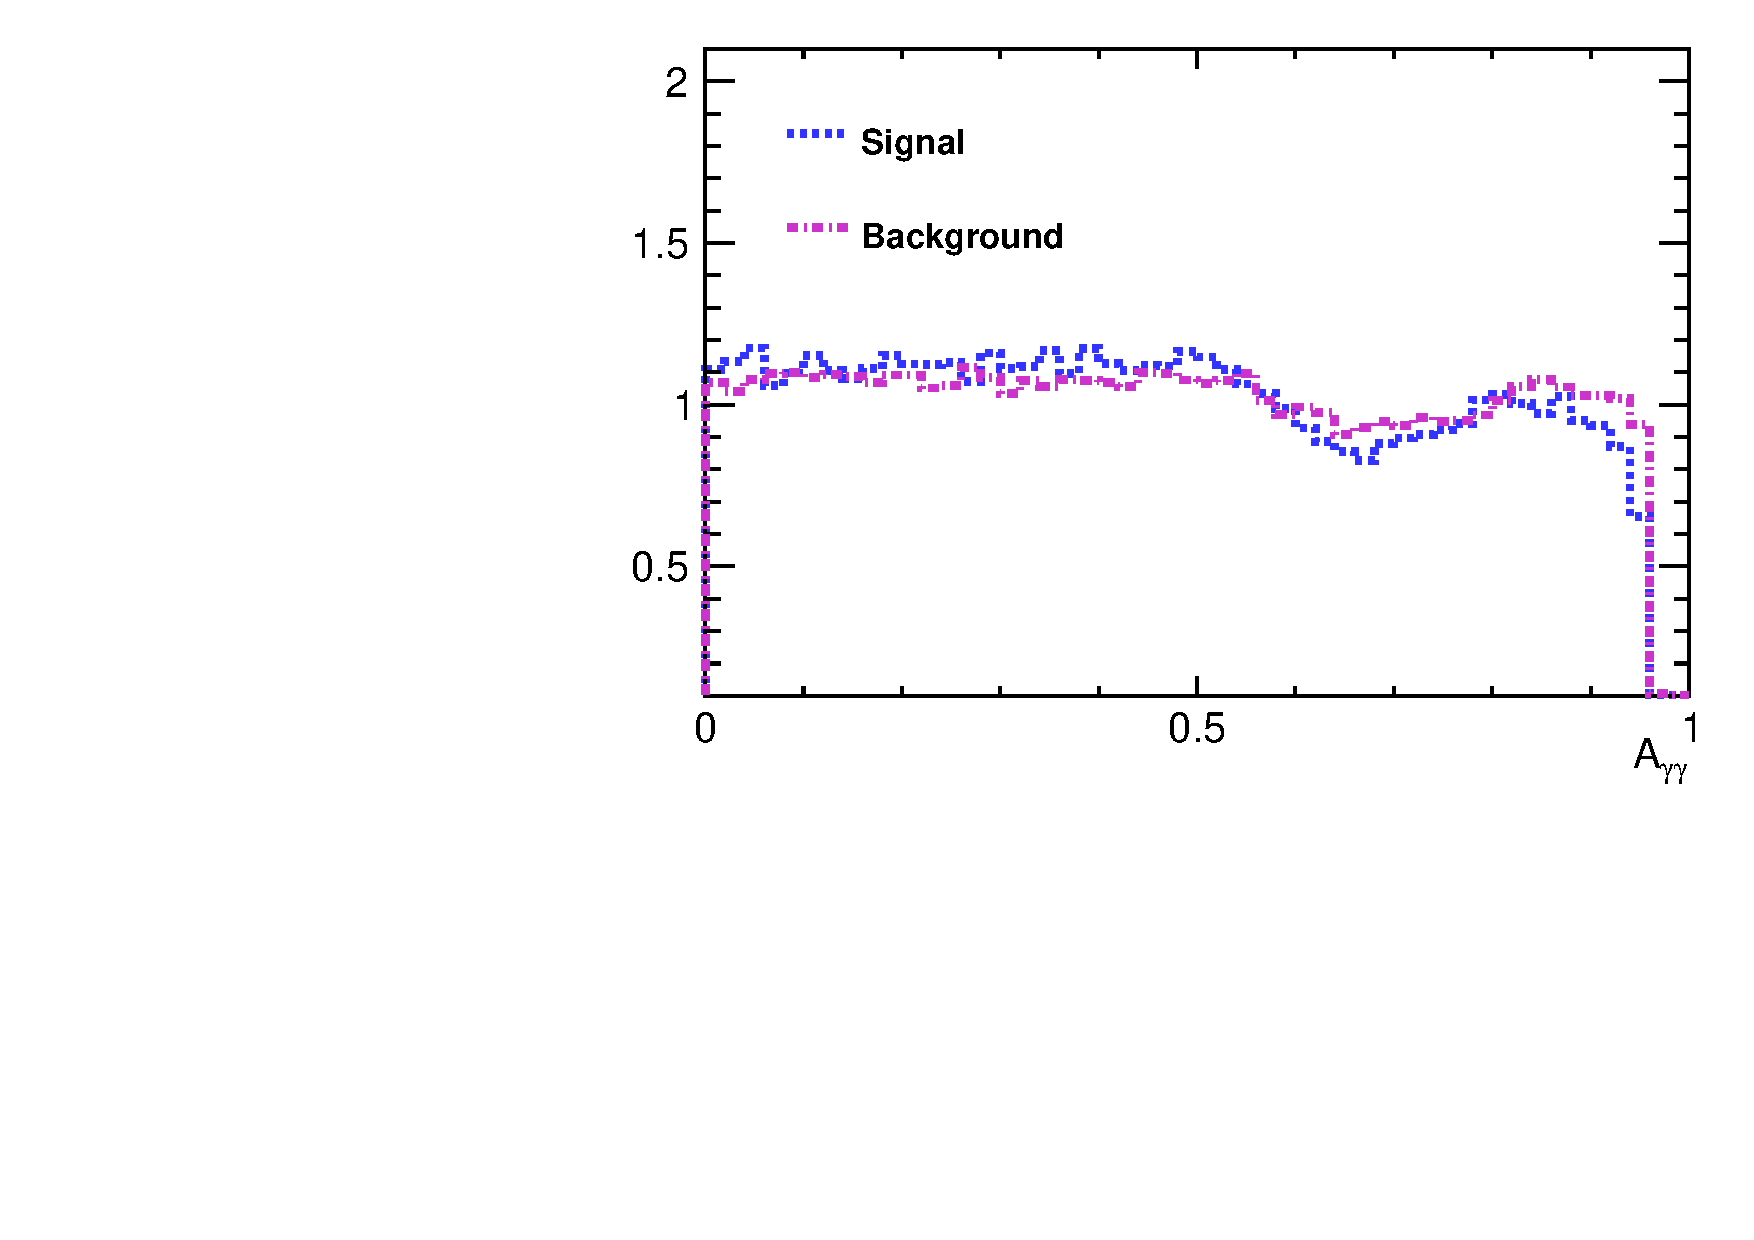
\includegraphics[width=.48\textwidth,natwidth=250,natheight=100]{figure_dataselection/pi0_asy_plot_Z3.pdf}}
  %\subfigure[]{\label{fig:photon_asymmetry2}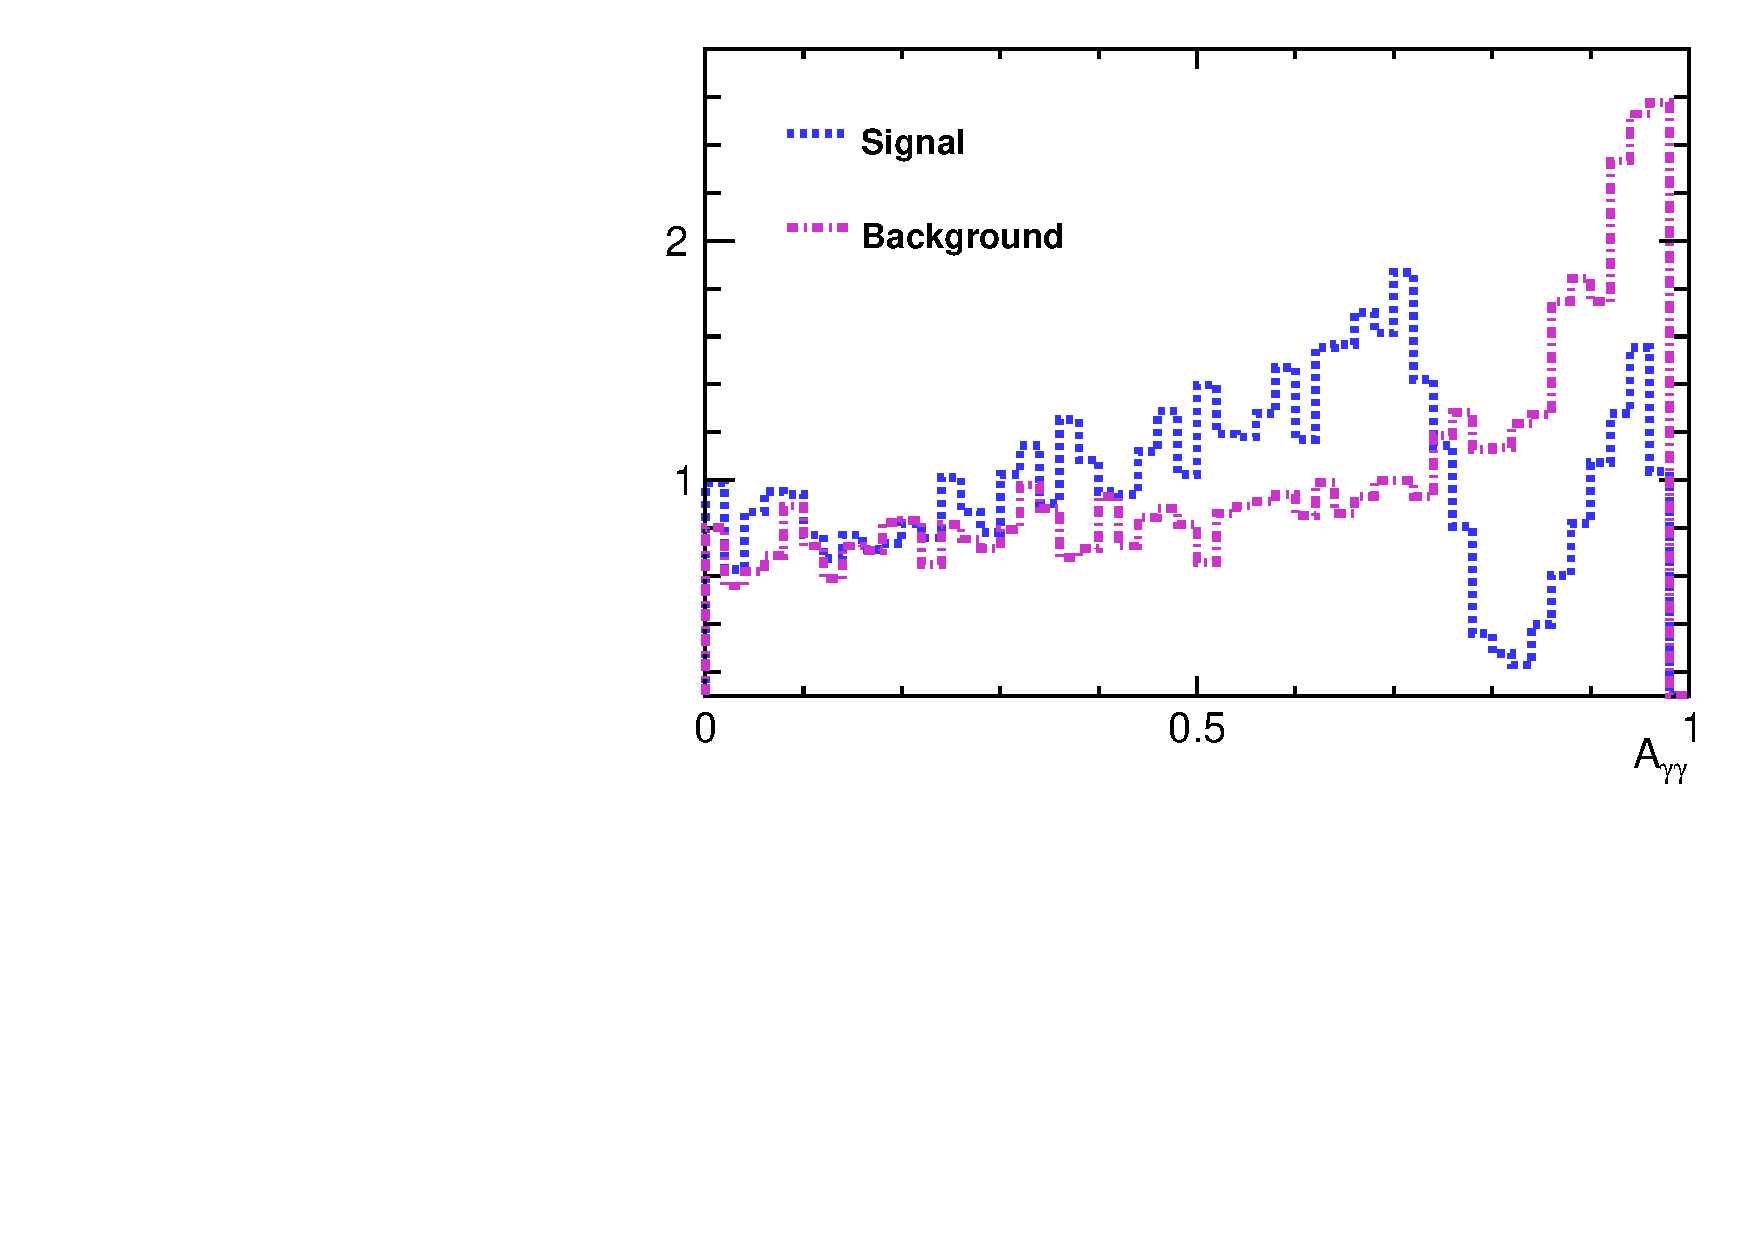
\includegraphics[width=.48\textwidth,natwidth=250,natheight=100]{figure_dataselection/pi0_asy_plot_Z6.pdf}}
 % \caption{Two examples of energy asymmetry $A_{\gamma\gamma}$. The left plot shows the $0.4<z<0.5$ bin and right plot the $0.7<z<1.0$ bin. In each plot, the blue line is the signal energy asymmetry andthe  purple line is the background energy asymmetry. To make the plots, the invariant mass of the reconstructed $\pi^0$ is restricted in the range of $0.1$~GeV$\textup{--}0.18$~GeV to avoid contribution of $\eta$ or other irrelevant background. As MC data is used in this plot, the signal and background events are distinguished by the particle ID of the reconstructed particles as well as the ID of their parents.}
%\label{fig:photon_asymmetry}
%\end{figure}

For the grid search discussed later, we consider the following bins in photon energy and photon energy asymmetry:
\begin{itemize}
  \item Photon Energy:
    \begin{itemize}
      \item $\pi^{0}$: $50$~MeV, $100$~MeV, $150$~MeV. 
      \item $\eta$: $150$~MeV, $200$~MeV, $250$~MeV, $300$~MeV, $400$~MeV. 
    \end{itemize}
  \item Photon Energy asymmetry $A_{\gamma\gamma}=\frac{|\gamma_1-\gamma_2|}{\gamma_1+\gamma_2}$ : $<0.8$ ,$<0.9$, $<1$.
\end{itemize}

\label{sec:energyconstraint}


\subsubsection{Fiducial Constraints}
\label{sec:fiducialcut}
Since we extract modulations that are only expected to be a few percent of the total cross-section, we restrict our analysis to parts of the detectors where the acceptance is smooth. This means, that we apply fiducial cuts that ensure that all $\gamma$'s are captured in the barrel EMCAL shown in Fig.~\ref{fig:2}. In the CMS, where we define our fiducial constraints, this corresponds to a cut on the polar angle of  hadrons and $\gamma$'s of $0.84<\theta<2.53$~rad, where $\theta$ is the angle between momentum direction and the $e^+e^-$ axis.
  In addition, because we are measuring azimuthal asymmetries around the thrust axis, we apply fiducial cuts on the opening angle (OA) of the detected hadrons/photons with respect to the thrust axis ($H_{OA}$ and $\gamma_{OA}$, respectively), such that the acceptance of the detector does not lead to false asymmetries. This is the case when the acceptance is azimuthally symmetric around the thrust axis for all allowed directions of that axis. This is illustrated in Fig.~\ref{fig:FiducialCut}. 

\begin{figure}[H]
  \centering
  \includegraphics[width=0.8\textwidth,natwidth=610,natheight=642]{figure_dataselection/EMCAL.pdf}
  %\includegraphics[scale=.3,keepaspectratio]{EMCAL.pdf}
  \caption{Configuration of Belle electromagnetic calorimeter~\cite{BelleDetector}}
  \label{fig:2}
\end{figure}

\begin{figure}[H]
  \centering
  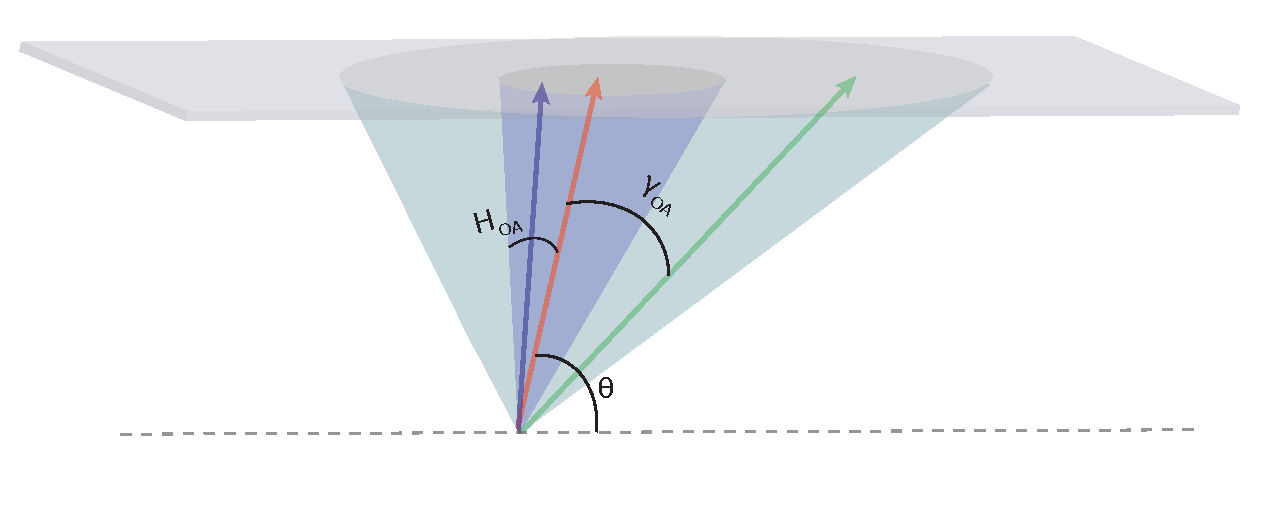
\includegraphics[width=0.95\textwidth,natwidth=610,natheight=642]{figure_dataselection/OA.pdf}
  \captionof{figure}{Illustration of the fiducial constraints in the CMS system. The red line represents the thrust axis, the green line a photon and the blue line a hadron. The cones represent the corresponding boundaries ($H_{OA}$ should be drawn between the hadron, not the blue boundary, and the thrust axis). The outer cone stand for the boundary of $\gamma$'s and the inner cone for hadrons. To make sure that all $\gamma$s are captured by the barrel EMCAL, the value of $\theta \pm \gamma_{OA}$ should fall in the range $0.84~\text{rad}<\theta\pm \gamma_{OA}<2.53~\text{rad}$. Here $\theta$ is again the angle between the $e^+e^-$ beam axis and the thrust axis in the CMS.}
  \label{fig:FiducialCut}
\end{figure}
 Given the fiducial cuts described above, the OA constraint also dictates the allowed range of the polar angle $\theta$ of the thrust axis to the beam axis in the CMS.  Even at maximal OA, tracks and photons have to be contained in the allowed polar-angle range given by the EMCAL acceptance. For example, if the maximum OA is $0.4$~rad, the thrust direction is limited within $1.24~\text{rad}<\theta<2.13~\text{rad}$.  A tighter boundary of OA leaves more room for thrust range at the expense of the yield of hadrons, and vice versa as shown in Fig.~\ref{fig:OAs}. For the grid search we use (in addition to the previously defined bins in photon energy and asymmetry) the following bins in the opening angle:
\begin{itemize}
\item Opening angle (OA): $<0.4$~rad, $<0.5$~rad, $<0.6$~rad.
\end{itemize}

As already indicated in~Fig.~\ref{fig:OAs}, we will eventually apply a tighter OA cut on hadrons than on the photons, since our goal is to have similar kinematics for charged and neutral hadrons and the decay photons of the neutral hadrons can occupy a larger OA than the parent hadron. In a first step we determine the optimal fiducial cuts using simulated data under the assumption that we will use the same cuts for$H_{OA}$ and $\gamma_{OA}$.  In a second step we choose a subset of the thus allowed phase space for $H_{OA}$ by applying tighter bounds to equalize the kinematic distributions between the different hadron species.

Table~\ref{tab:FOM} shows the optimized constraints for each kinematic bin. Most bins of $\pi^0$ have the same optimized constraints, namely the photon energy threshold of $50$~MeV, no photon energy asymmetry cut and an OA constraint of $0.5$, and these constraints are chosen as our data selection criteria. For other bins, comparisons are made to confirm that the FOMs of selected criteria of that bin approximate the optimized FOM. The same approach is used for $\eta$ and the final selection criteria can be found in Table~\ref{tab:constrain}.%includes the photon energy threshold $250$~MeV, no photon energy asymmetry cut and OA constraint $0.5$. With $z<0.3$ the purity of $\eta$ is below $30\%$ and thus it is required that $z>0.3$ for $\eta$ mesons. 
\begin{table}[H]
\begin{tabular}{|p{1.3cm}|l|l|l|l|l|l|l|l|l|l|l|l|l|}
\hline
Bin & $E_{\gamma}$~MeV & $A_{\gamma\gamma}$ & OA \\ \hline
$z_0$ & 0.05 & 0.8 & 0.6 \\\hline
$z_1$ & 0.05 & 0.9 & 0.5 \\\hline
$z_2$ & 0.05 & 1 & 0.5 \\\hline
$z_3$ & 0.05 & 1 & 0.5 \\\hline
$z_4$ & 0.10 & 1 & 0.5 \\\hline
$z_5$ & 0.05 & 1 & 0.5 \\\hline
$z_6$ & 0.05 & 1 & 0.5 \\\hline
$P_{t0}$ & 0.05 & 1 & 0.5 \\\hline
$P_{t1}$ & 0.05 & 1 & 0.5 \\\hline
$P_{t2}$ & 0.10 & 1 & 0.5 \\\hline
$P_{t3}$ & 0.05 & 1 & 0.6 \\\hline
\end{tabular}
%\caption{Constraints that generate optimized FOM for $\pi^{0}$.}
%\label{tab:pi0FOM}
\quad
\begin{tabular}{|p{1.3cm}|l|l|l|l|l|l|l|l|l|l|l|l|l|}
\hline
Bin & $E_{\gamma}$~MeV & $A_{\gamma\gamma}$ & OA \\ \hline
$z_0$ &  &  &  \\\hline
$z_1$ &  &  &  \\\hline
$z_2$ & 0.15 & 1 & 0.5 \\\hline
$z_3$ & 0.25 & 1 & 0.5 \\\hline
$z_4$ & 0.25 & 1 & 0.5 \\\hline
$z_5$ & 0.25 & 1 & 0.5 \\\hline
$z_6$ & 0.25 & 1 & 0.5 \\\hline
$P_{t0}$ & 0.20 & 1 & 0.5 \\\hline
$P_{t1}$ & 0.20 & 1 & 0.5 \\\hline
$P_{t2}$ & 0.15 & 1 & 0.5 \\\hline
$P_{t3}$ & 0.25 & 1 & 0.5 \\\hline
\end{tabular}
\caption{Constraints that generate optimized FOM for $\pi^0$~(left) and $\eta$~(right).}
\label{tab:FOM}
\end{table}


\begin{figure}[h]
  \centering     %%% not \center
  \subfigure[$\pi^0$ to thrust angle]{\label{fig:a}\includegraphics[width=60mm]{figure_dataselection/pi0_OA.eps}}
  \subfigure[$\eta$ to thrust angle]{\label{fig:b}\includegraphics[width=60mm]{figure_dataselection/eta_OA.eps}}
  \caption{$H_{OA}$ distribution under various $\gamma_{OA}$ constraints; the different color lines represent different $\gamma_{OA}$ constraints. The constraints are meant to be symmetric between the hemispheres, i.e. if  $\gamma_{OA}> \pi/2$ the constraint is on $\pi-\gamma_{OA} $.  For example, the $\gamma_{OA}$ constraint forthe red solid line is 0.3~rad. It can be seen that with the decrease of the $\gamma$ range, the width of the hadron distribution becomes thinner.}
  \label{fig:OAs}
\end{figure}



%Fig.~\ref{fig:FiducialCut} shows the hadron/photon to thrust opening angles that will be used to do fiducial constraint. Our previous study shows that the optimized criteria for OA is $0.5$ for hadrons/photons. 
In addition to avoid false asymmetries, the opening angle cut has to be chosen to match the $p_T$ and $z$ distributions between the neutral and charged hadrons used in the double ratio. Otherwise, the double ratio would be difficult to interpret, since the integration ranges for the different contributing hadrons in $p_T$ and $z$ would be different. Additionally, the cancellation of detector effects in the double ratio would not be guaranteed.
%However, the main motivation behind the opening cut is the goal to equalize the observed kinematic distributions between neutral and charged mesons. Given that the underlying distributions of $p_T$ and $z$ should be very similar, matching observed distributions for these variables imply matching detection efficiencies. This in turn is a prerequisite to successfully apply the double ratio method which is used to cancel detector effects.
 In \cref{fig:kine_distri1,fig:kine_distri2,fig:kine_distri3,fig:kine_distri4} we compare different, tighter, $H_{OA}$ constraints, where we leave $\gamma_{OA}$ at the previously determined optimum of $\gamma_{OA}<0.5$.
  As expected, we see better agreement of the kinematic distribution of pions under tighter $H_{OA}$ constraints. More plots can be found in section~\ref{sec:kinedistri_pi0}~\ref{sec:kinedistri_eta}.
\begin{figure}[H]
\captionsetup[subfloat]{farskip=2pt,captionskip=1pt}
\centering
\subfigure[$H_{OA}<0.3$]{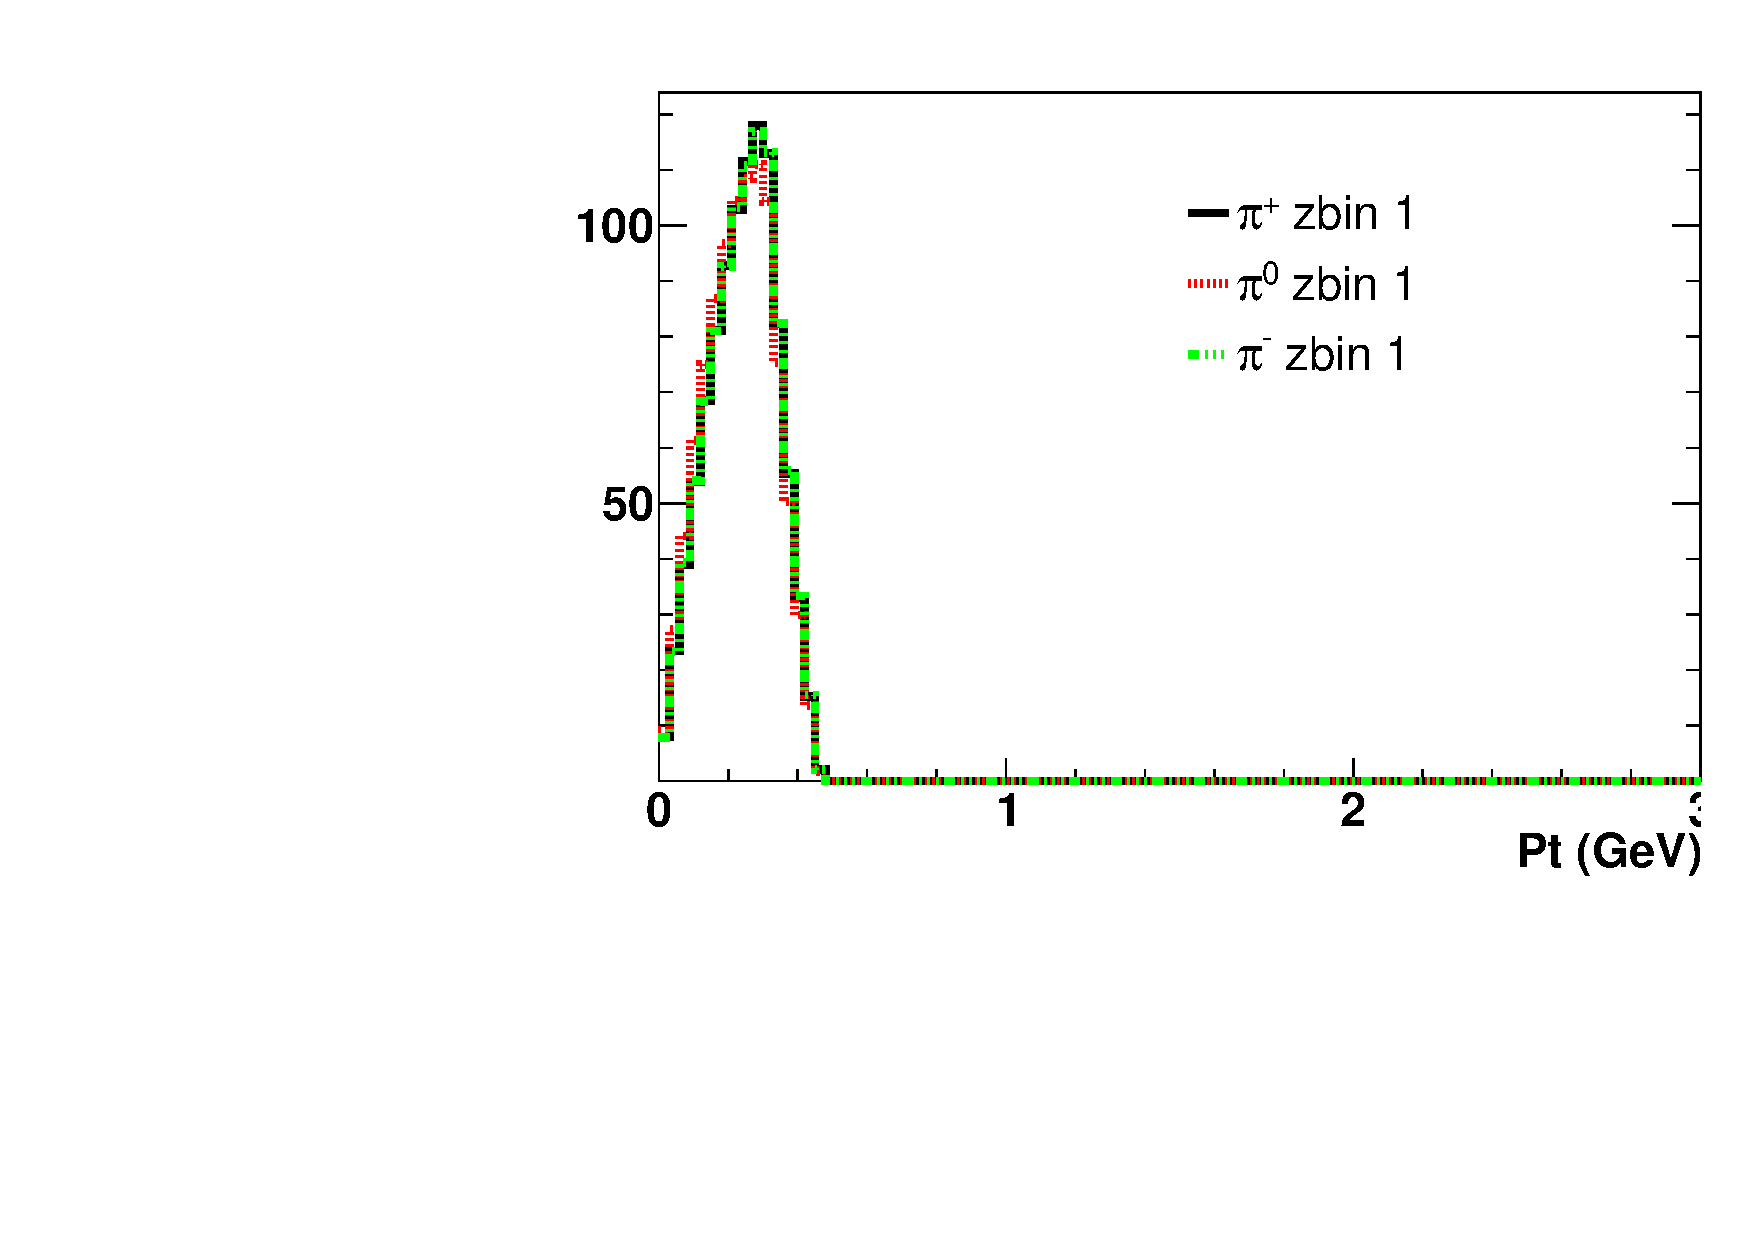
\includegraphics[width=.31\textwidth,natwidth=250,natheight=100]{figure_fiducial/had0.3/Pt_distri_for_zbin_1_norm_had03.pdf}\label{fig:kine_distri11}}
\subfigure[$H_{OA}<0.4$]{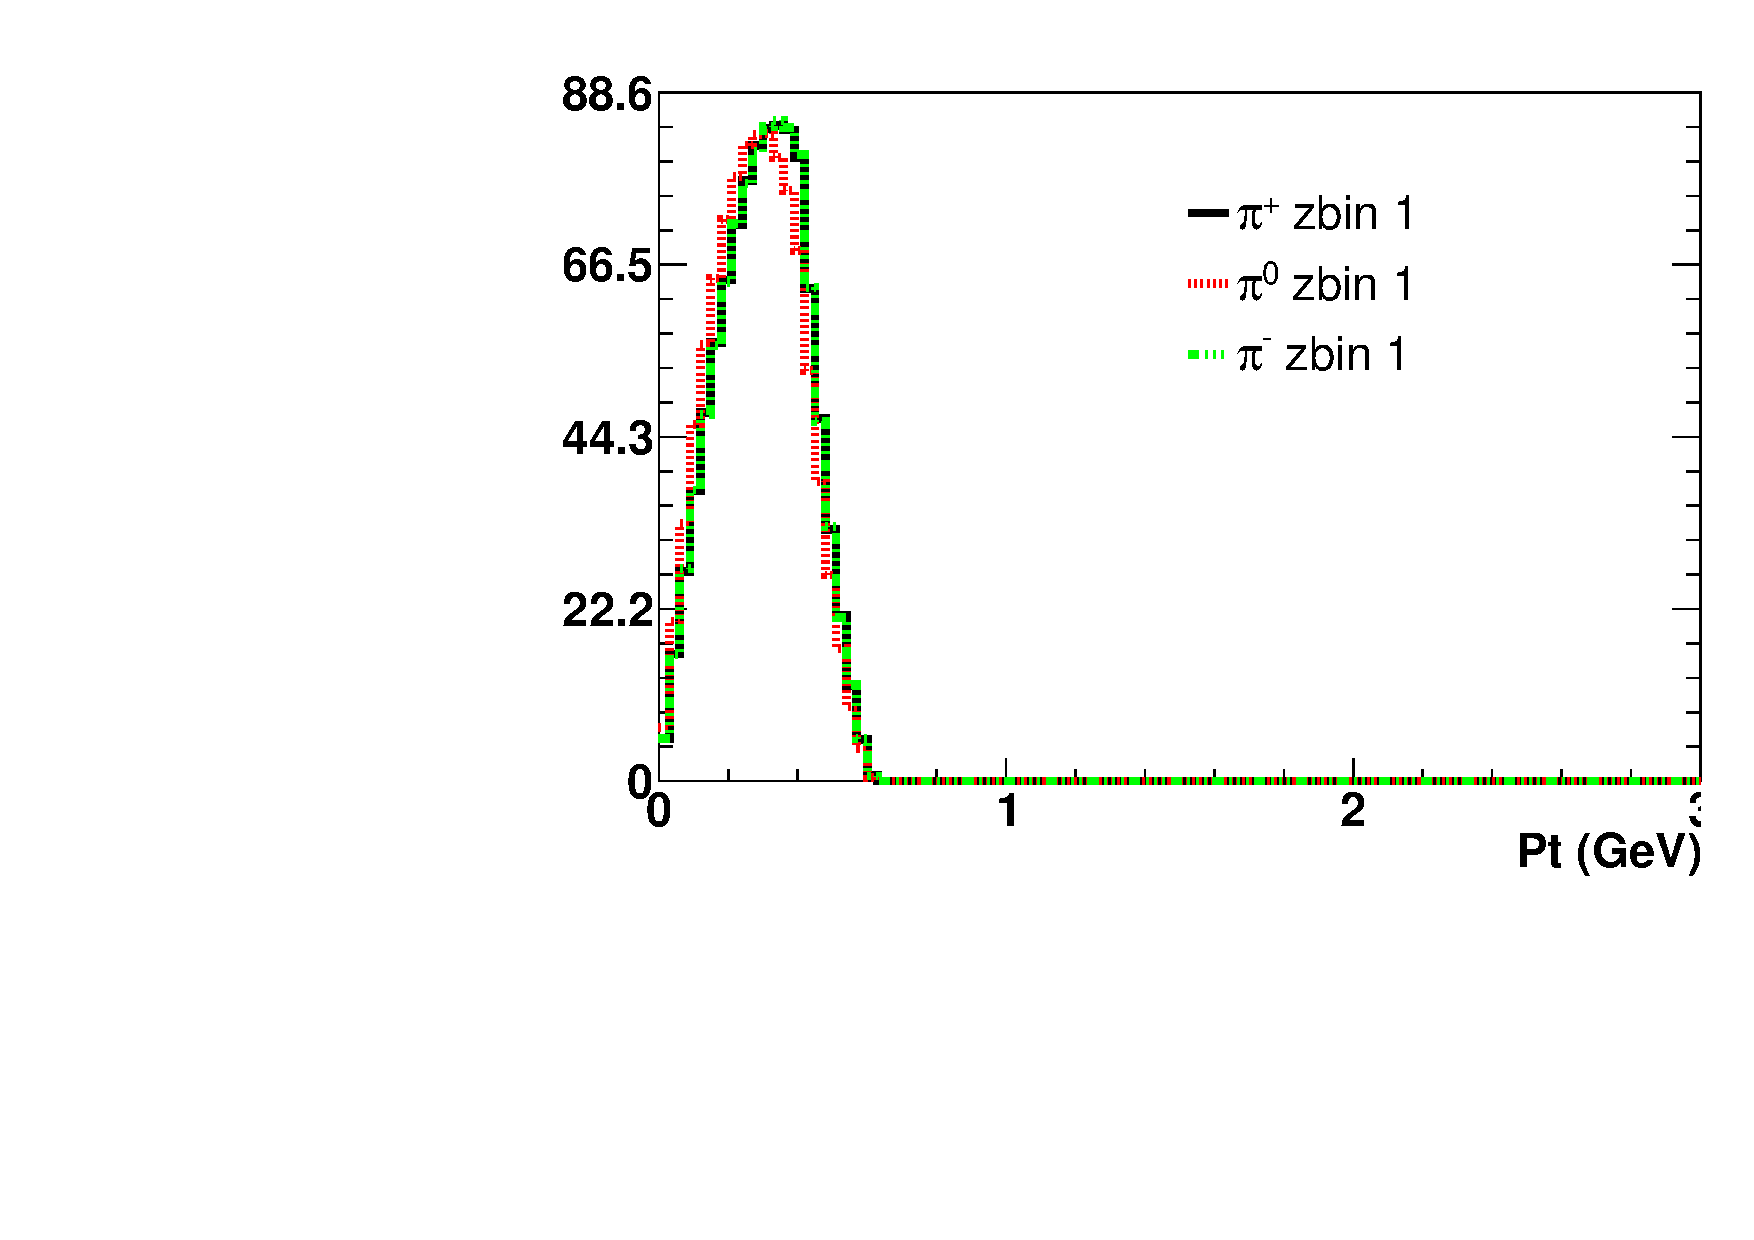
\includegraphics[width=.31\textwidth,natwidth=250,natheight=100]{figure_fiducial/had0.4/Pt_distri_for_zbin_1_norm_had04.pdf}\label{fig:kine_distri12}}
\subfigure[$H_{OA}<0.5$]{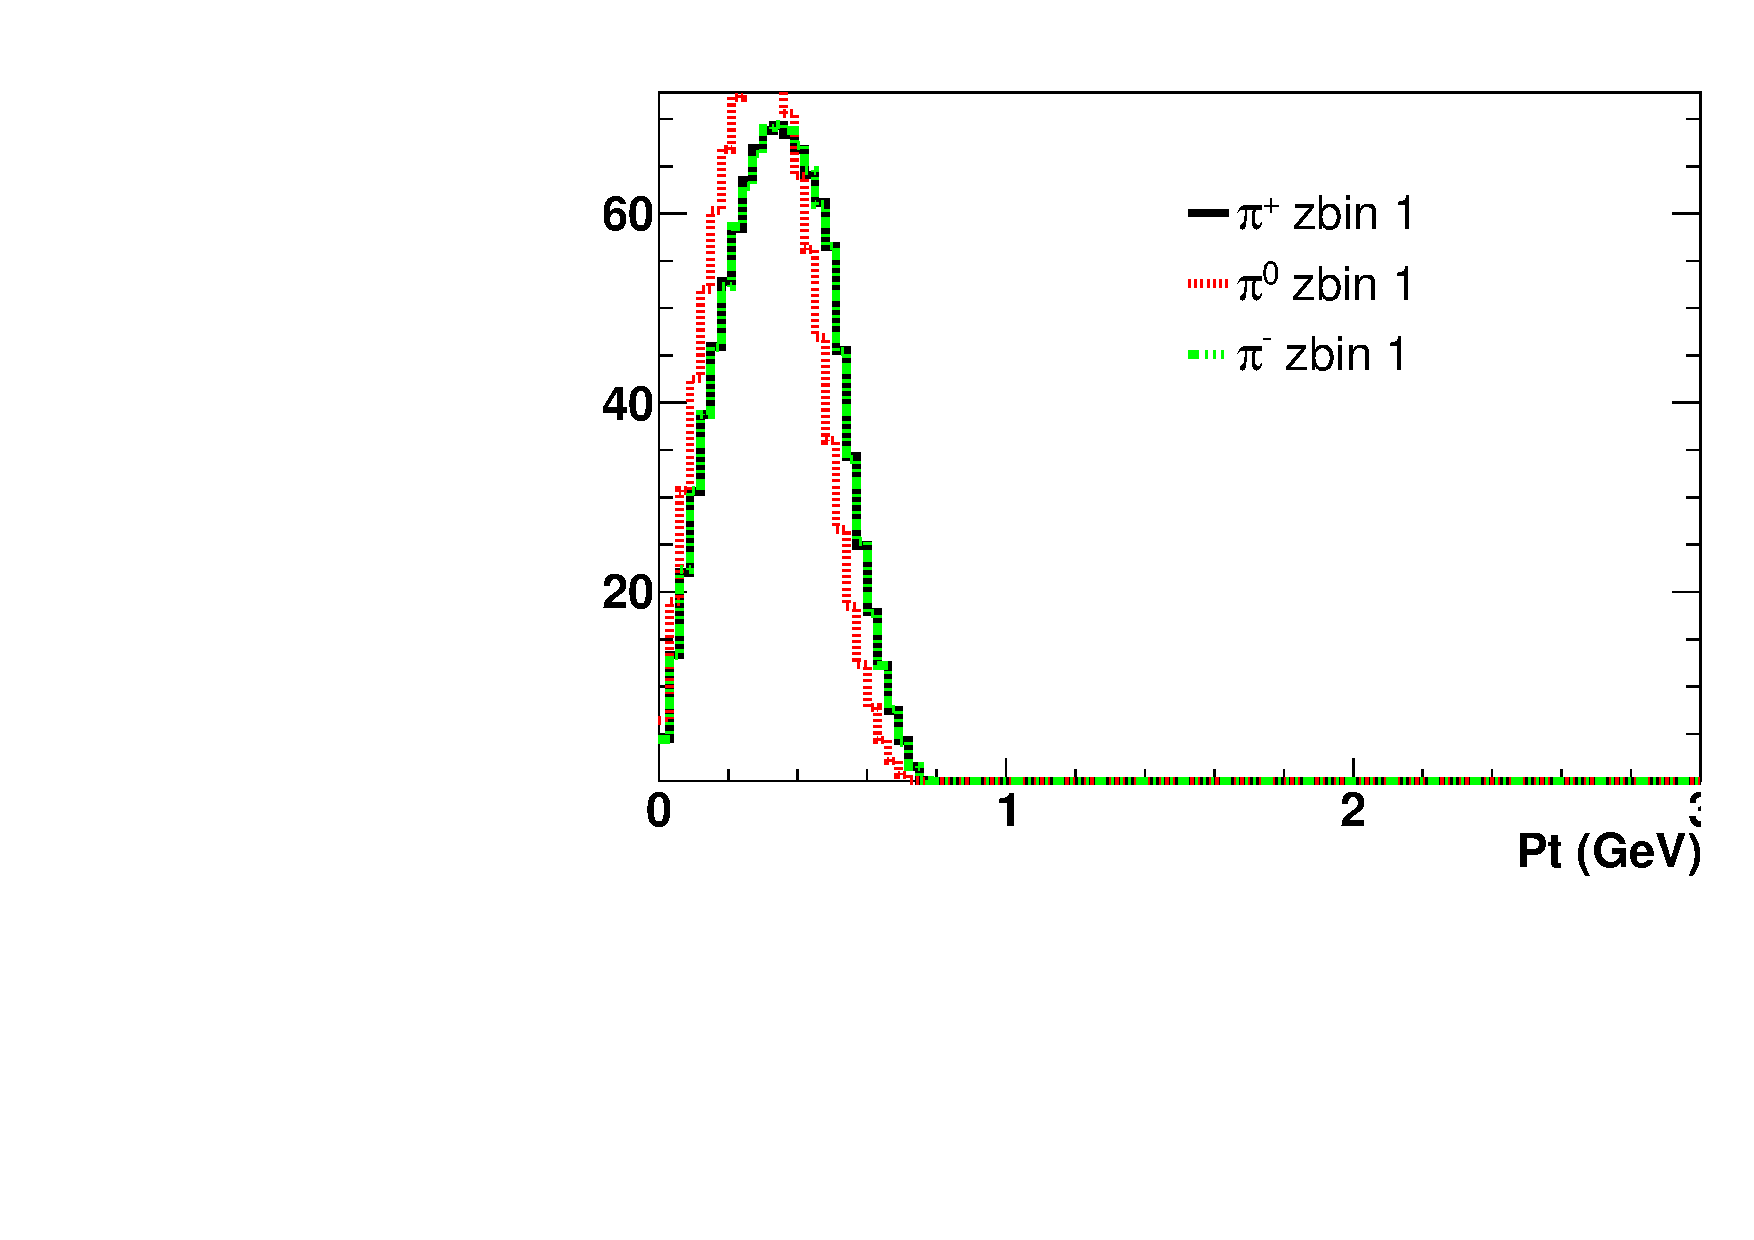
\includegraphics[width=.31\textwidth,natwidth=250,natheight=100]{figure_fiducial/had0.5/Pt_distri_for_zbin_1_norm_had05.pdf}\label{fig:kine_distri13}}
\caption{Normalized $P_t$ distribution of pions for $0.2<z<0.3$}
\label{fig:kine_distri1}
\end{figure}

\begin{figure}[H]
\captionsetup[subfloat]{farskip=2pt,captionskip=1pt}
\centering
\subfigure[$H_{OA}<0.3$]{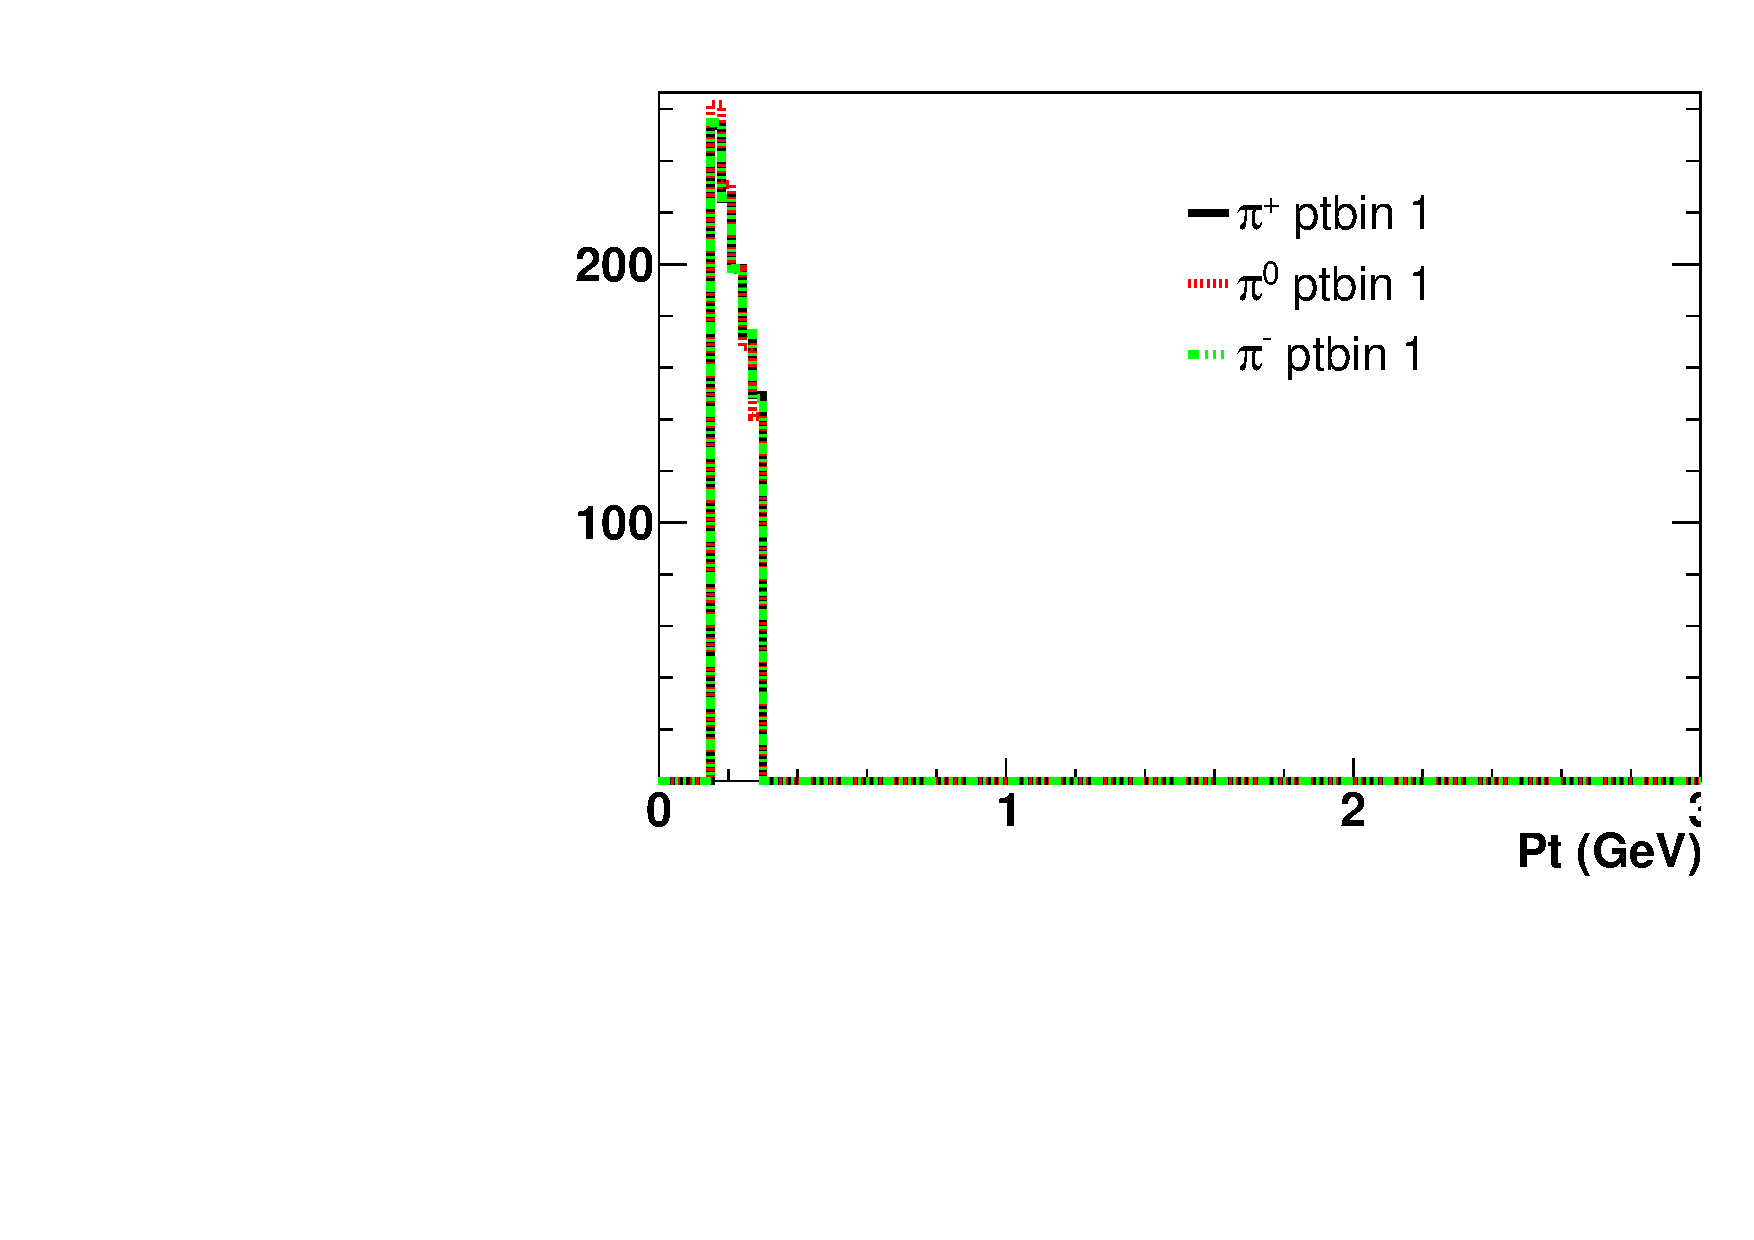
\includegraphics[width=.31\textwidth,natwidth=250,natheight=100]{figure_fiducial/had0.3/Pt_distri_for_ptbin_1_norm_had03.pdf}\label{fig:kine_distri21}}
\subfigure[$H_{OA}<0.4$]{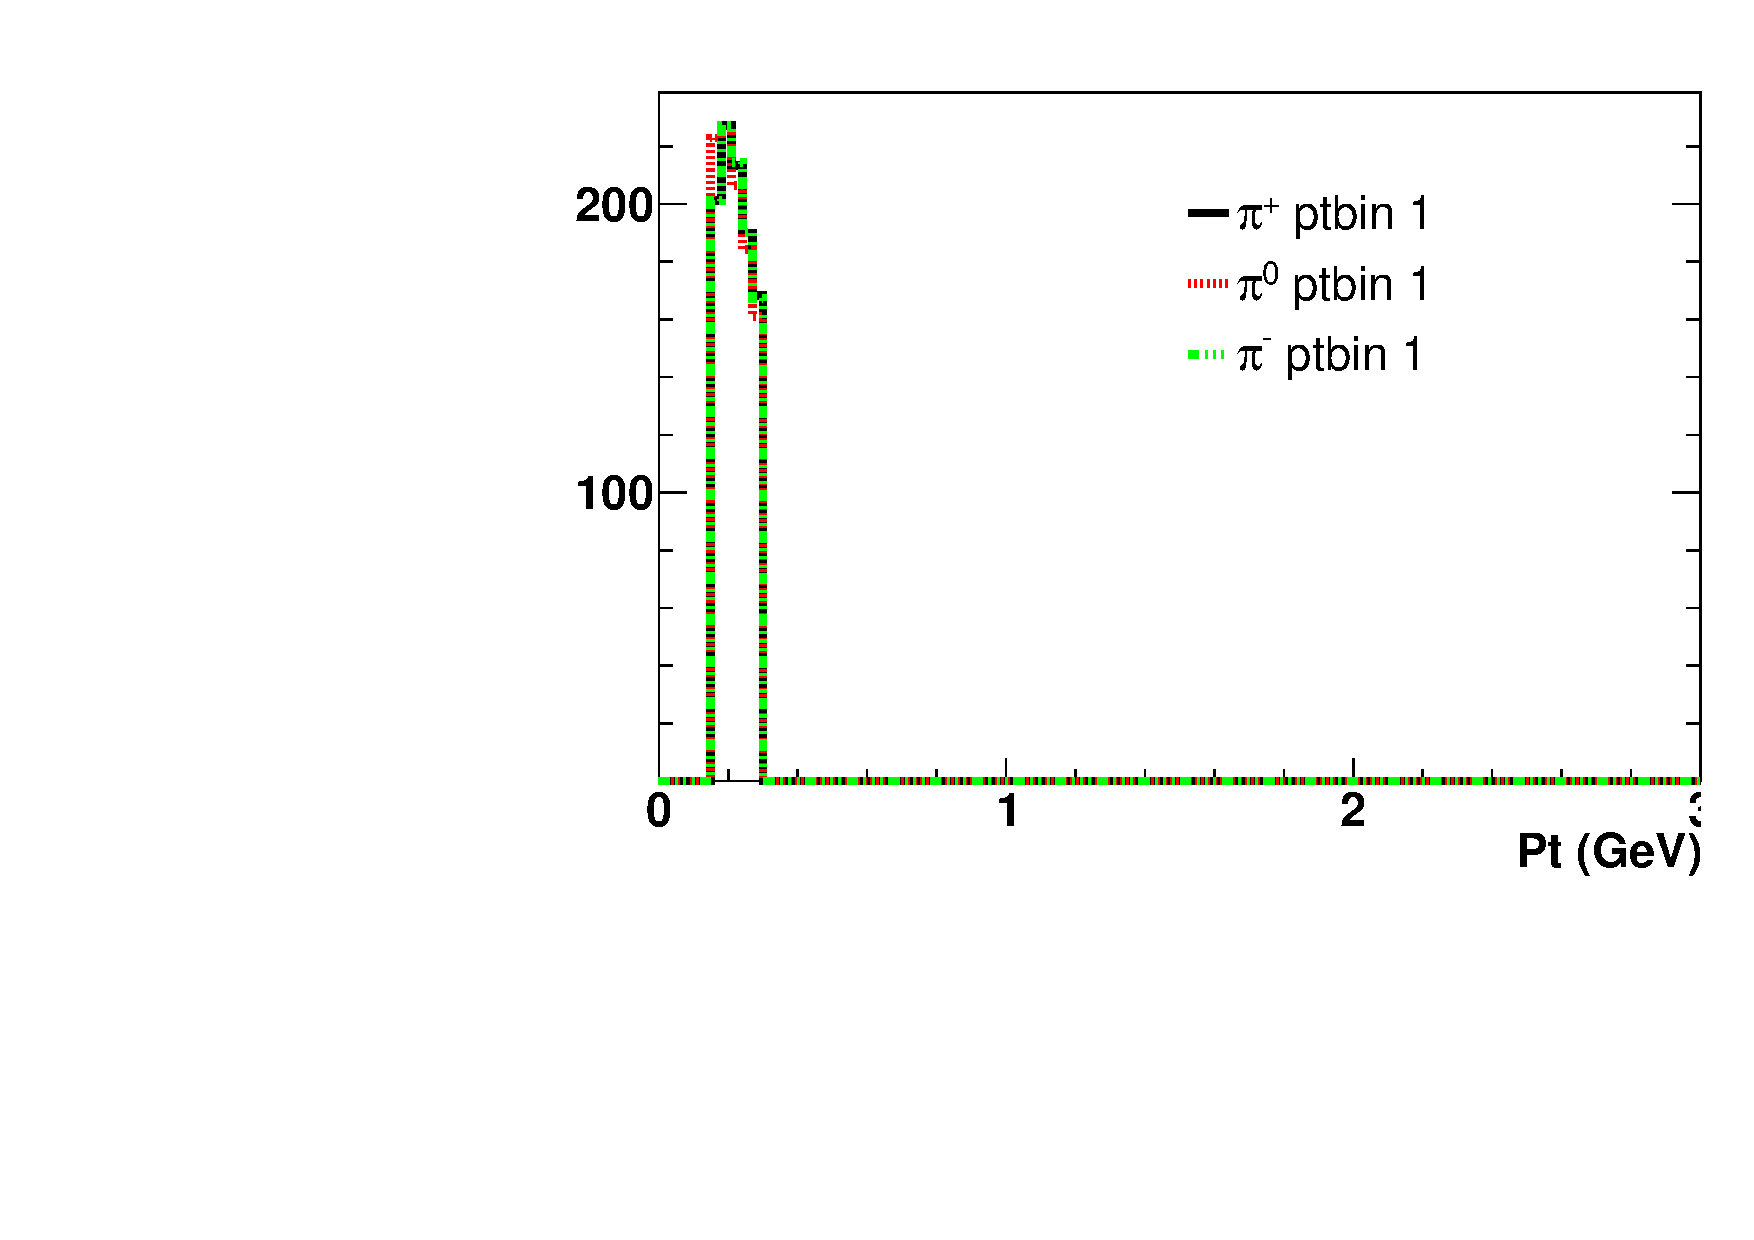
\includegraphics[width=.31\textwidth,natwidth=250,natheight=100]{figure_fiducial/had0.4/Pt_distri_for_ptbin_1_norm_had04.pdf}\label{fig:kine_distri22}}
\subfigure[$H_{OA}<0.5$]{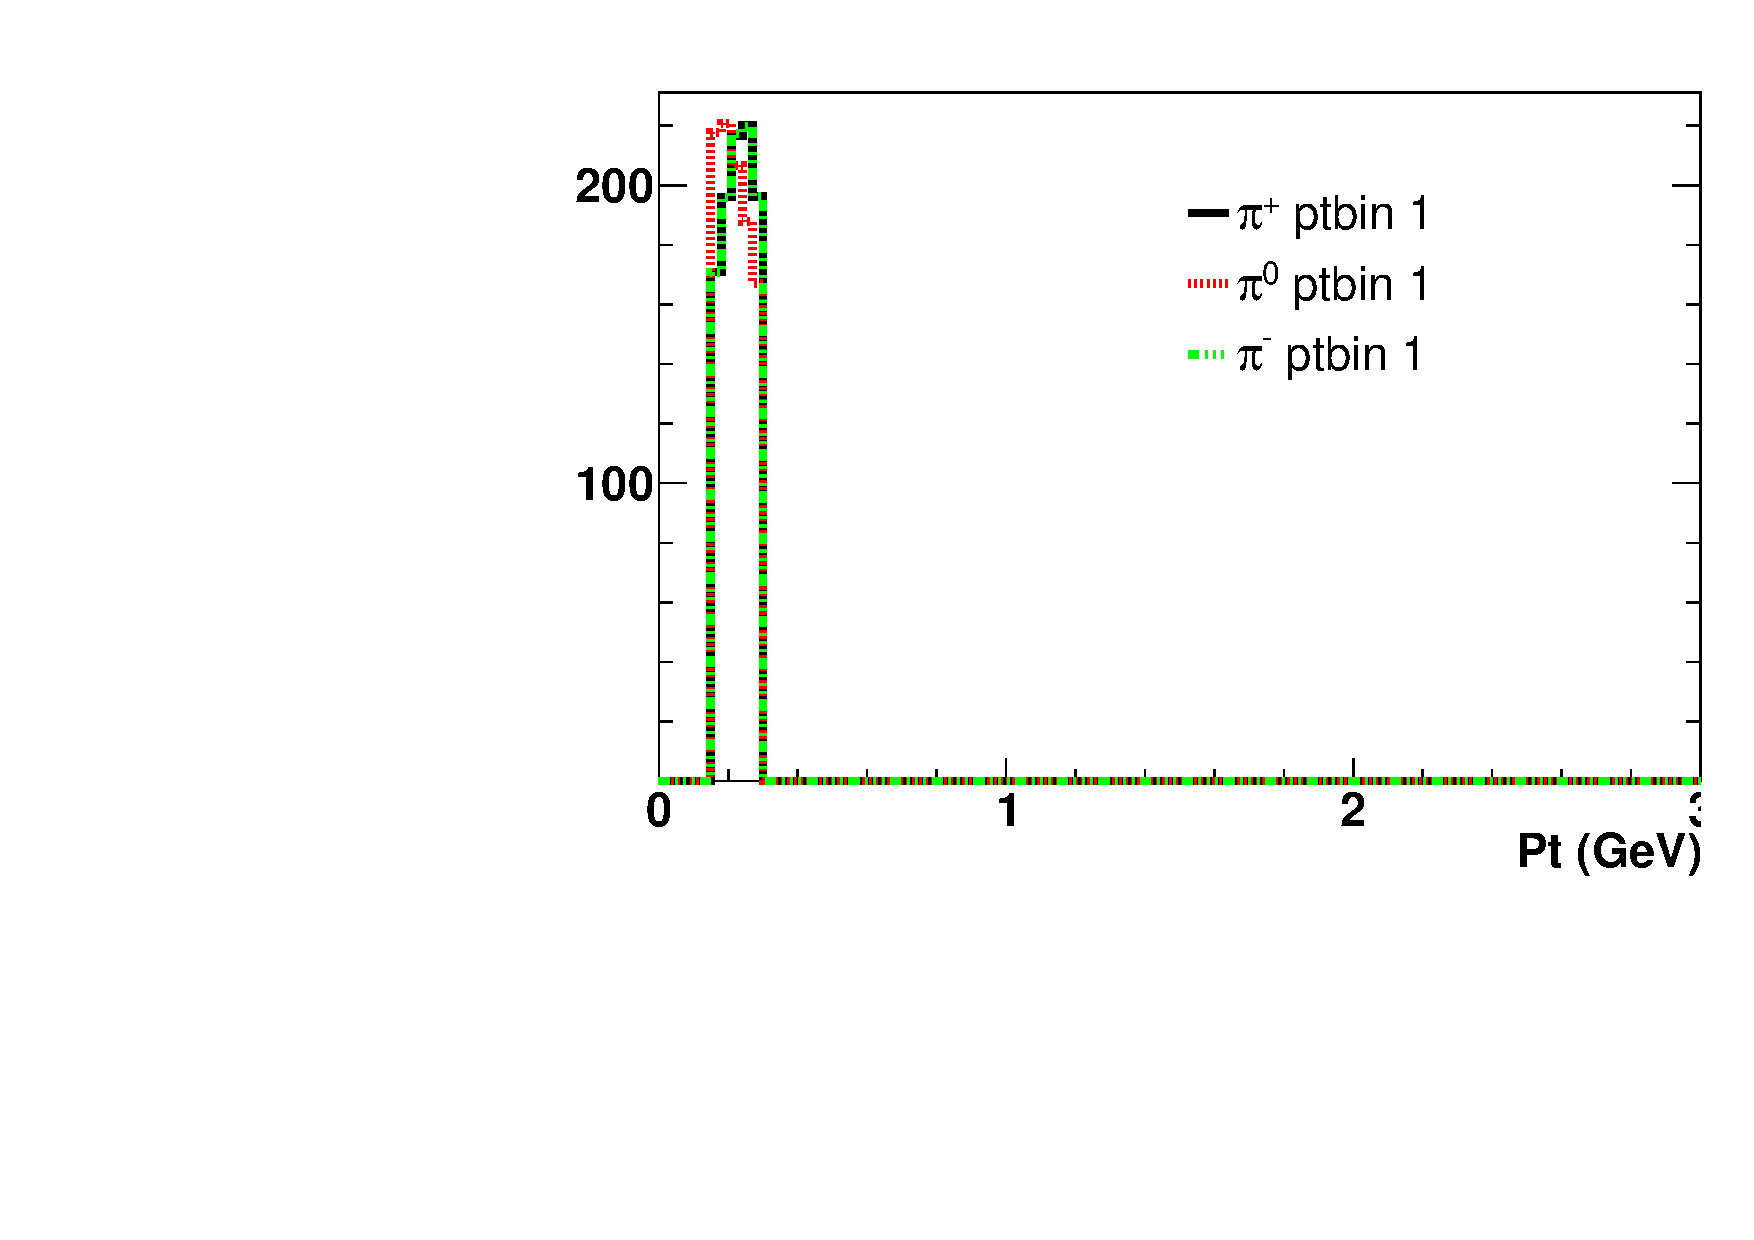
\includegraphics[width=.31\textwidth,natwidth=250,natheight=100]{figure_fiducial/had0.5/Pt_distri_for_ptbin_1_norm_had05.pdf}\label{fig:kine_distri23}}
\caption{Normalized $P_t$ distribution of pions for $0<P_{t}<0.15$}
\label{fig:kine_distri2}
\end{figure}

\begin{figure}[H]
\captionsetup[subfloat]{farskip=2pt,captionskip=1pt}
\centering
\subfigure[$H_{OA}<0.3$]{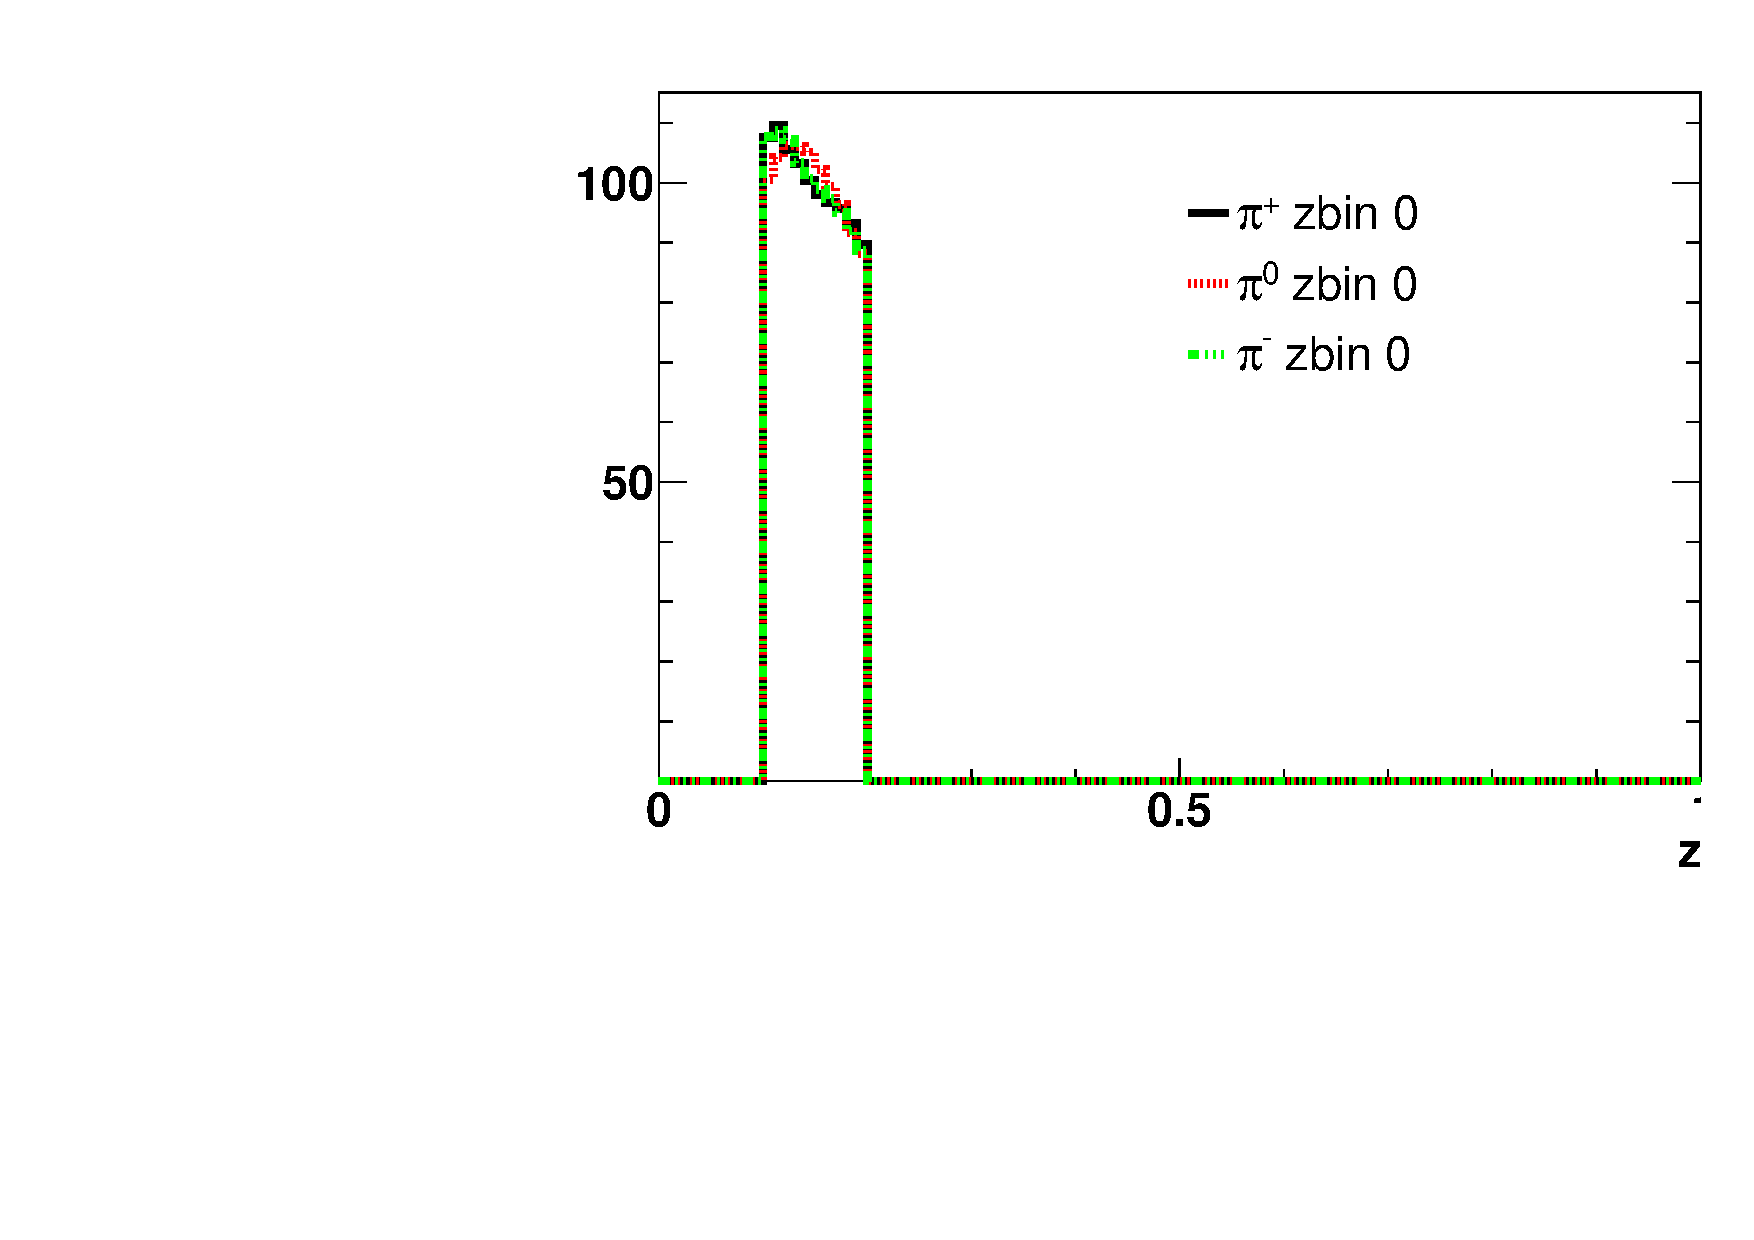
\includegraphics[width=.31\textwidth,natwidth=250,natheight=100]{figure_fiducial/had0.3/Z_distri_for_zbin_0_norm_had03.pdf}\label{fig:kine_distri31}}
\subfigure[$H_{OA}<0.4$]{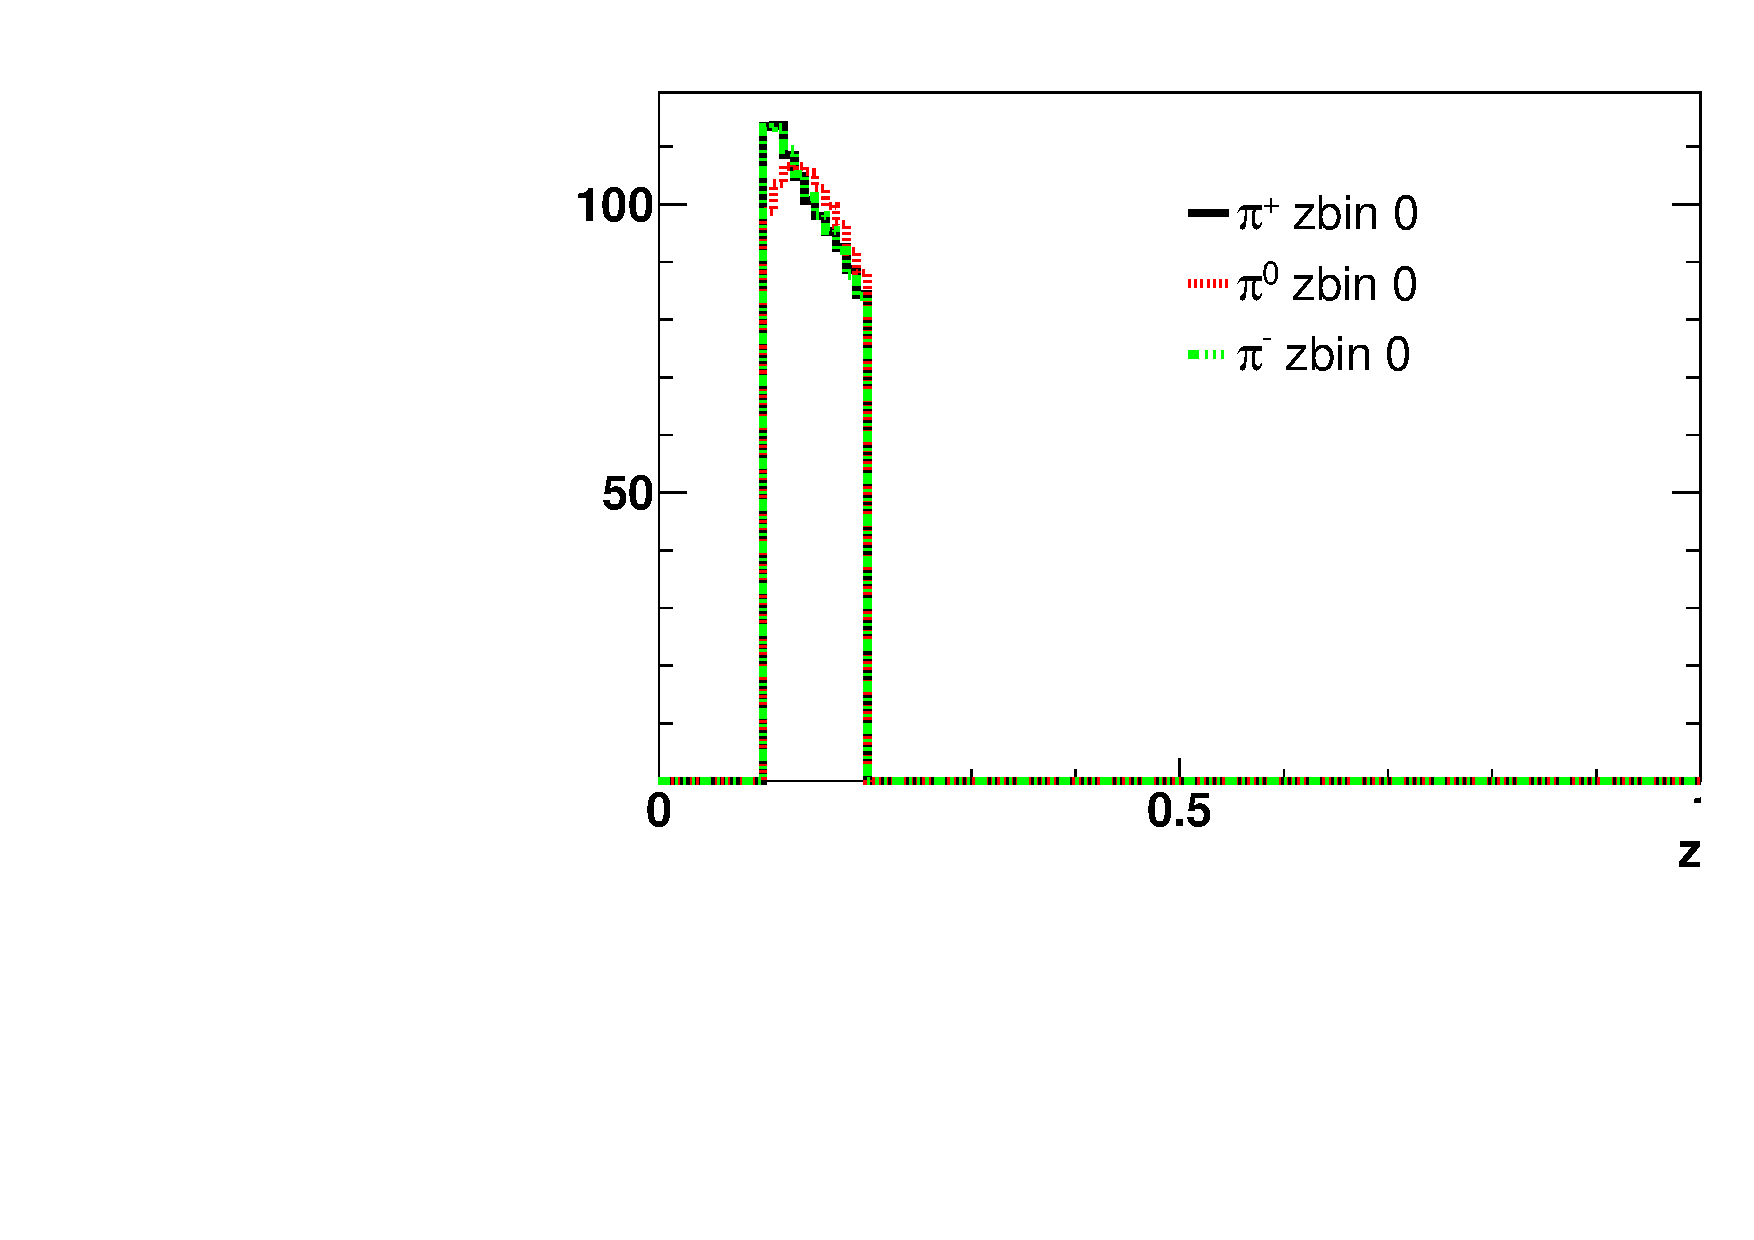
\includegraphics[width=.31\textwidth,natwidth=250,natheight=100]{figure_fiducial/had0.4/Z_distri_for_zbin_0_norm_had04.pdf}\label{fig:kine_distri32}}
\subfigure[$H_{OA}<0.5$]{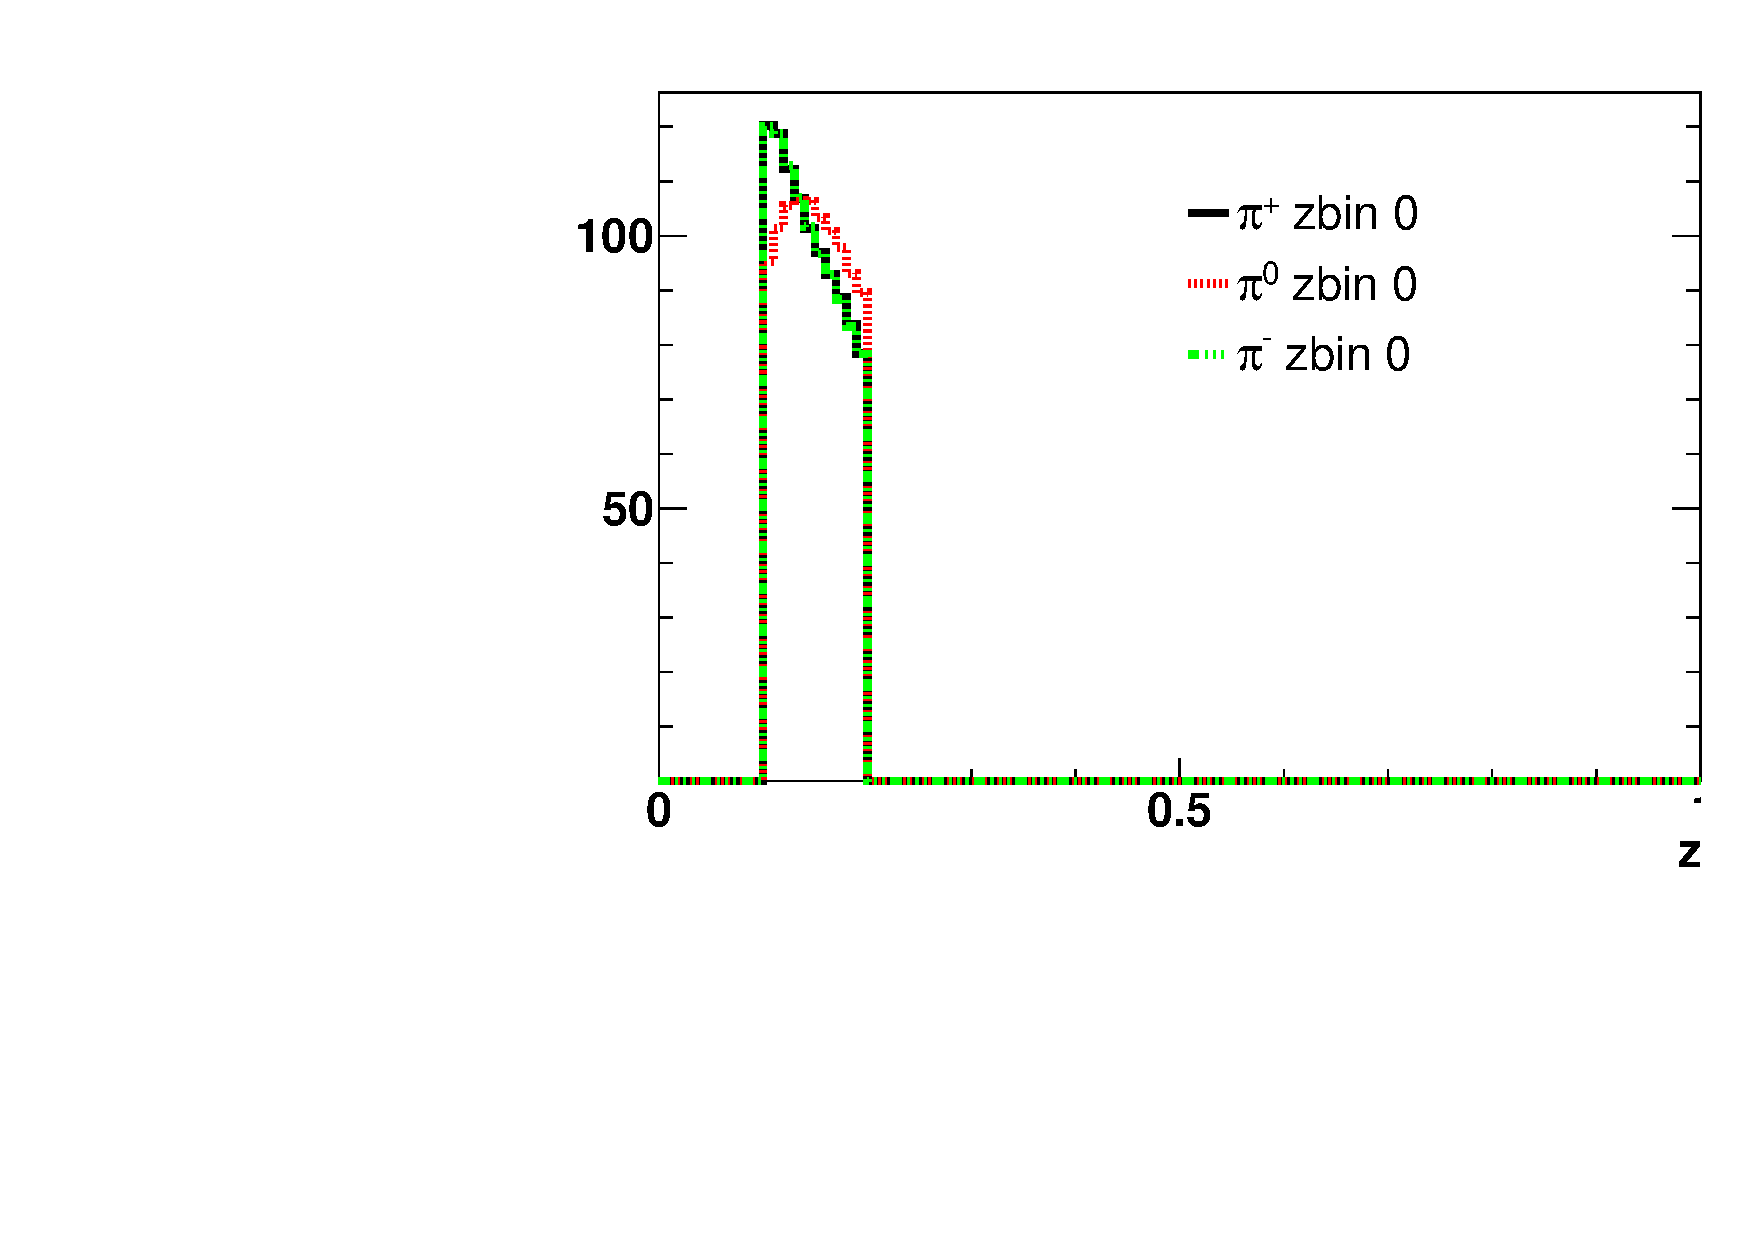
\includegraphics[width=.31\textwidth,natwidth=250,natheight=100]{figure_fiducial/had0.5/Z_distri_for_zbin_0_norm_had05.pdf}\label{fig:kine_distri33}}
\caption{Normalized $z$ distribution of pions for $0.1<z<0.2$}
\label{fig:kine_distri3}
\end{figure}

\begin{figure}[H]
\captionsetup[subfloat]{farskip=2pt,captionskip=1pt}
\centering
\subfigure[$H_{OA}<0.3$]{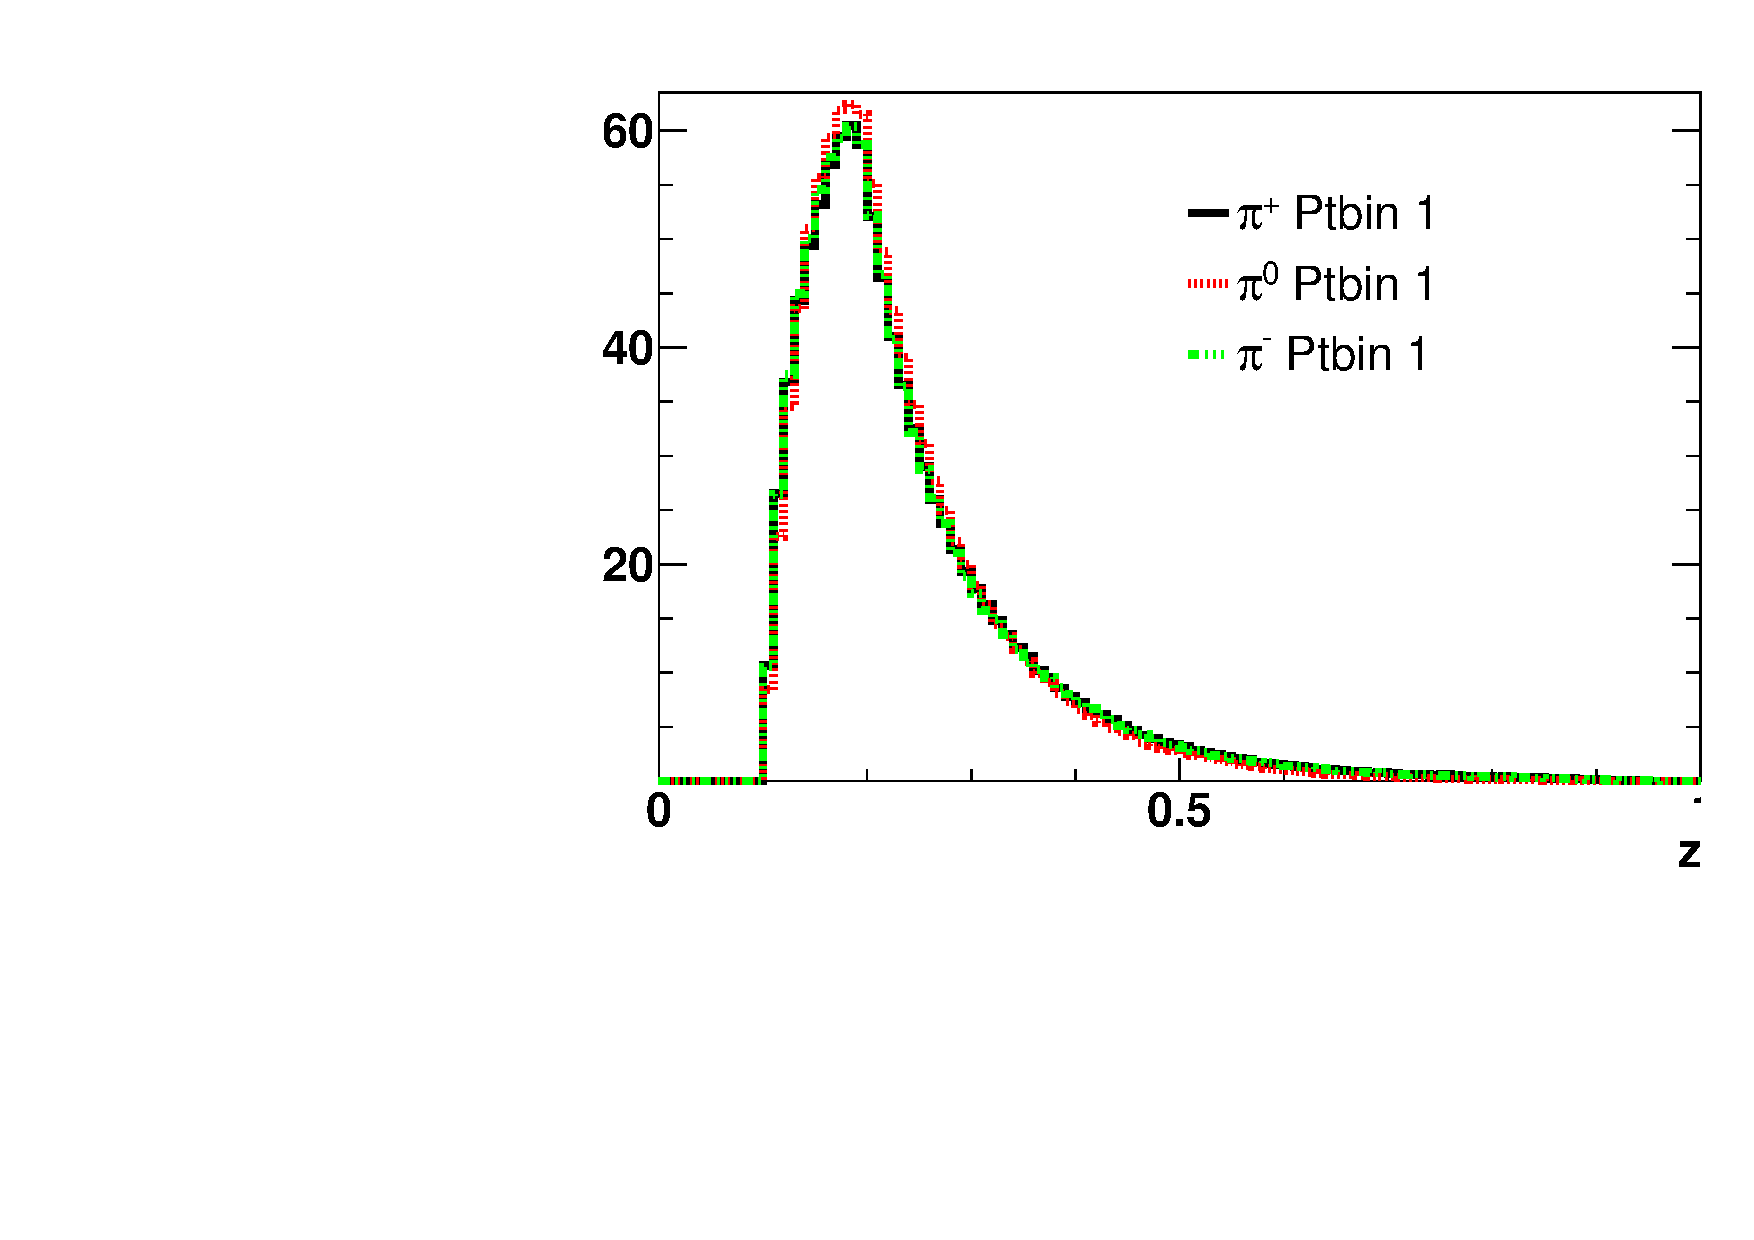
\includegraphics[width=.31\textwidth,natwidth=250,natheight=100]{figure_fiducial/had0.3/Z_distri_for_ptbin_1_norm_had03.pdf}\label{fig:kine_distri41}}
\subfigure[$H_{OA}<0.4$]{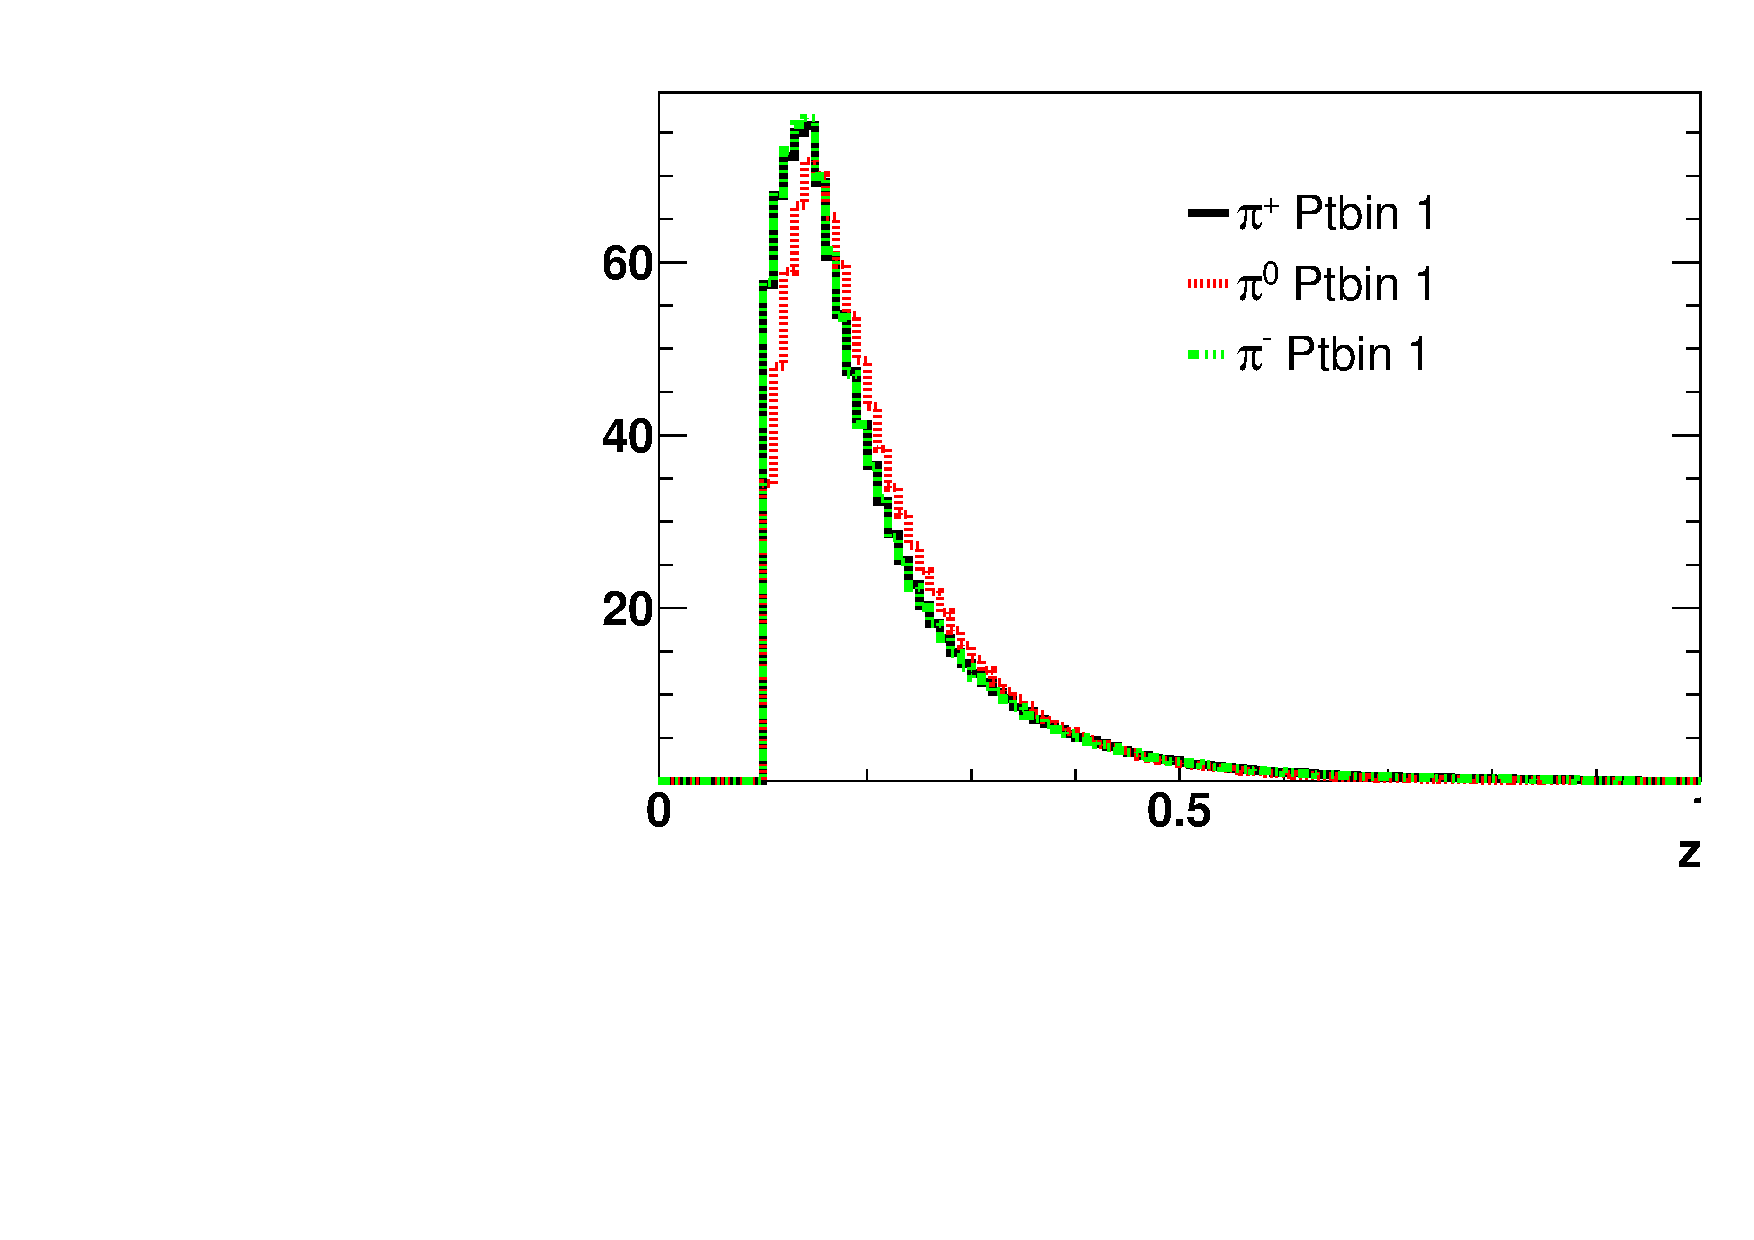
\includegraphics[width=.31\textwidth,natwidth=250,natheight=100]{figure_fiducial/had0.4/Z_distri_for_ptbin_1_norm_had04.pdf}\label{fig:kine_distri42}}
\subfigure[$H_{OA}<0.5$]{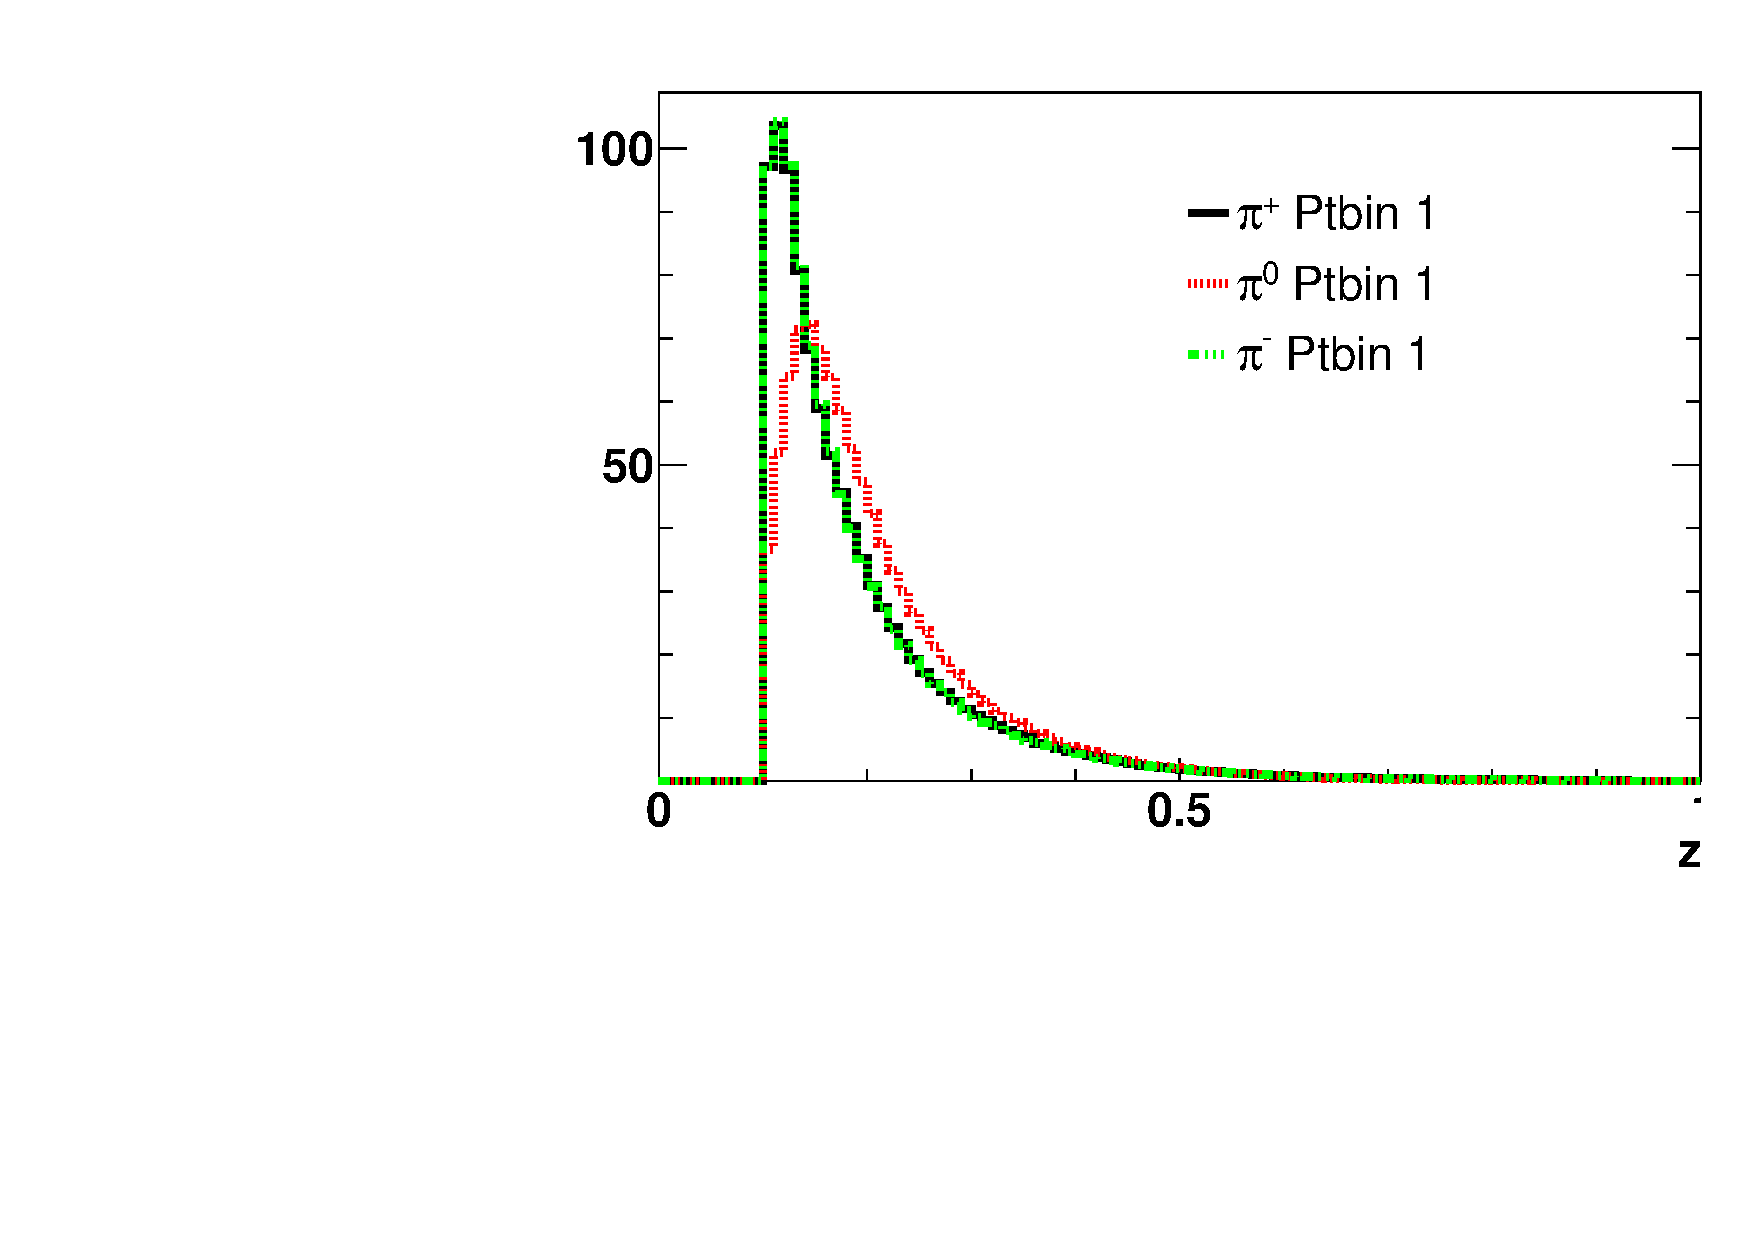
\includegraphics[width=.31\textwidth,natwidth=250,natheight=100]{figure_fiducial/had0.5/Z_distri_for_ptbin_1_norm_had05.pdf}\label{fig:kine_distri43}}
\caption{Normalized $z$ distribution of pions for $0.15<P_t<0.3$}
\label{fig:kine_distri4}
\end{figure}

\begin{figure}[H]
\captionsetup[subfloat]{farskip=2pt,captionskip=1pt}
\centering
\subfigure[$H_{OA}<0.3$]{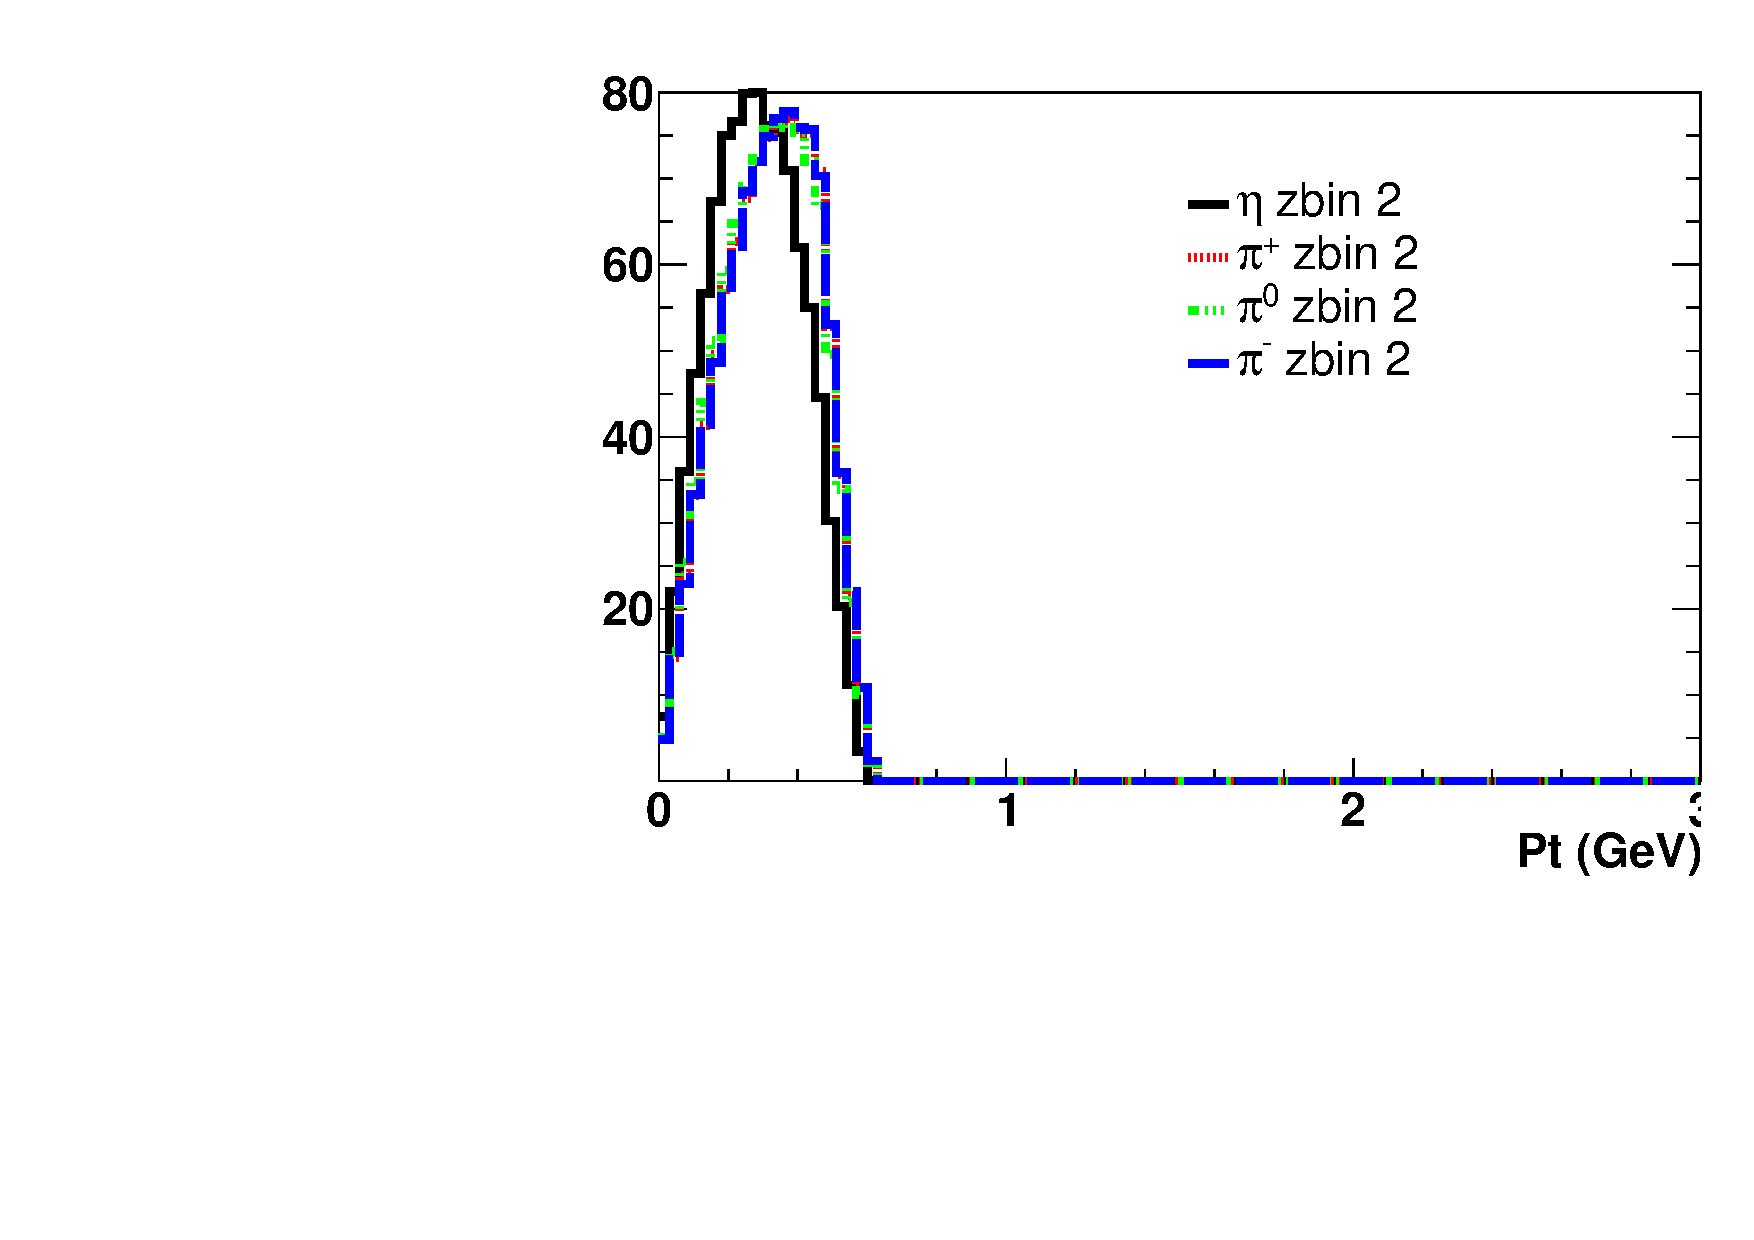
\includegraphics[width=.31\textwidth,natwidth=250,natheight=100]{figure_fiducial/had0.3_z0.3/Pt_distri_for_zbin_2_norm_had03z03.pdf}\label{fig:kine_distri51}}
\subfigure[$H_{OA}<0.4$]{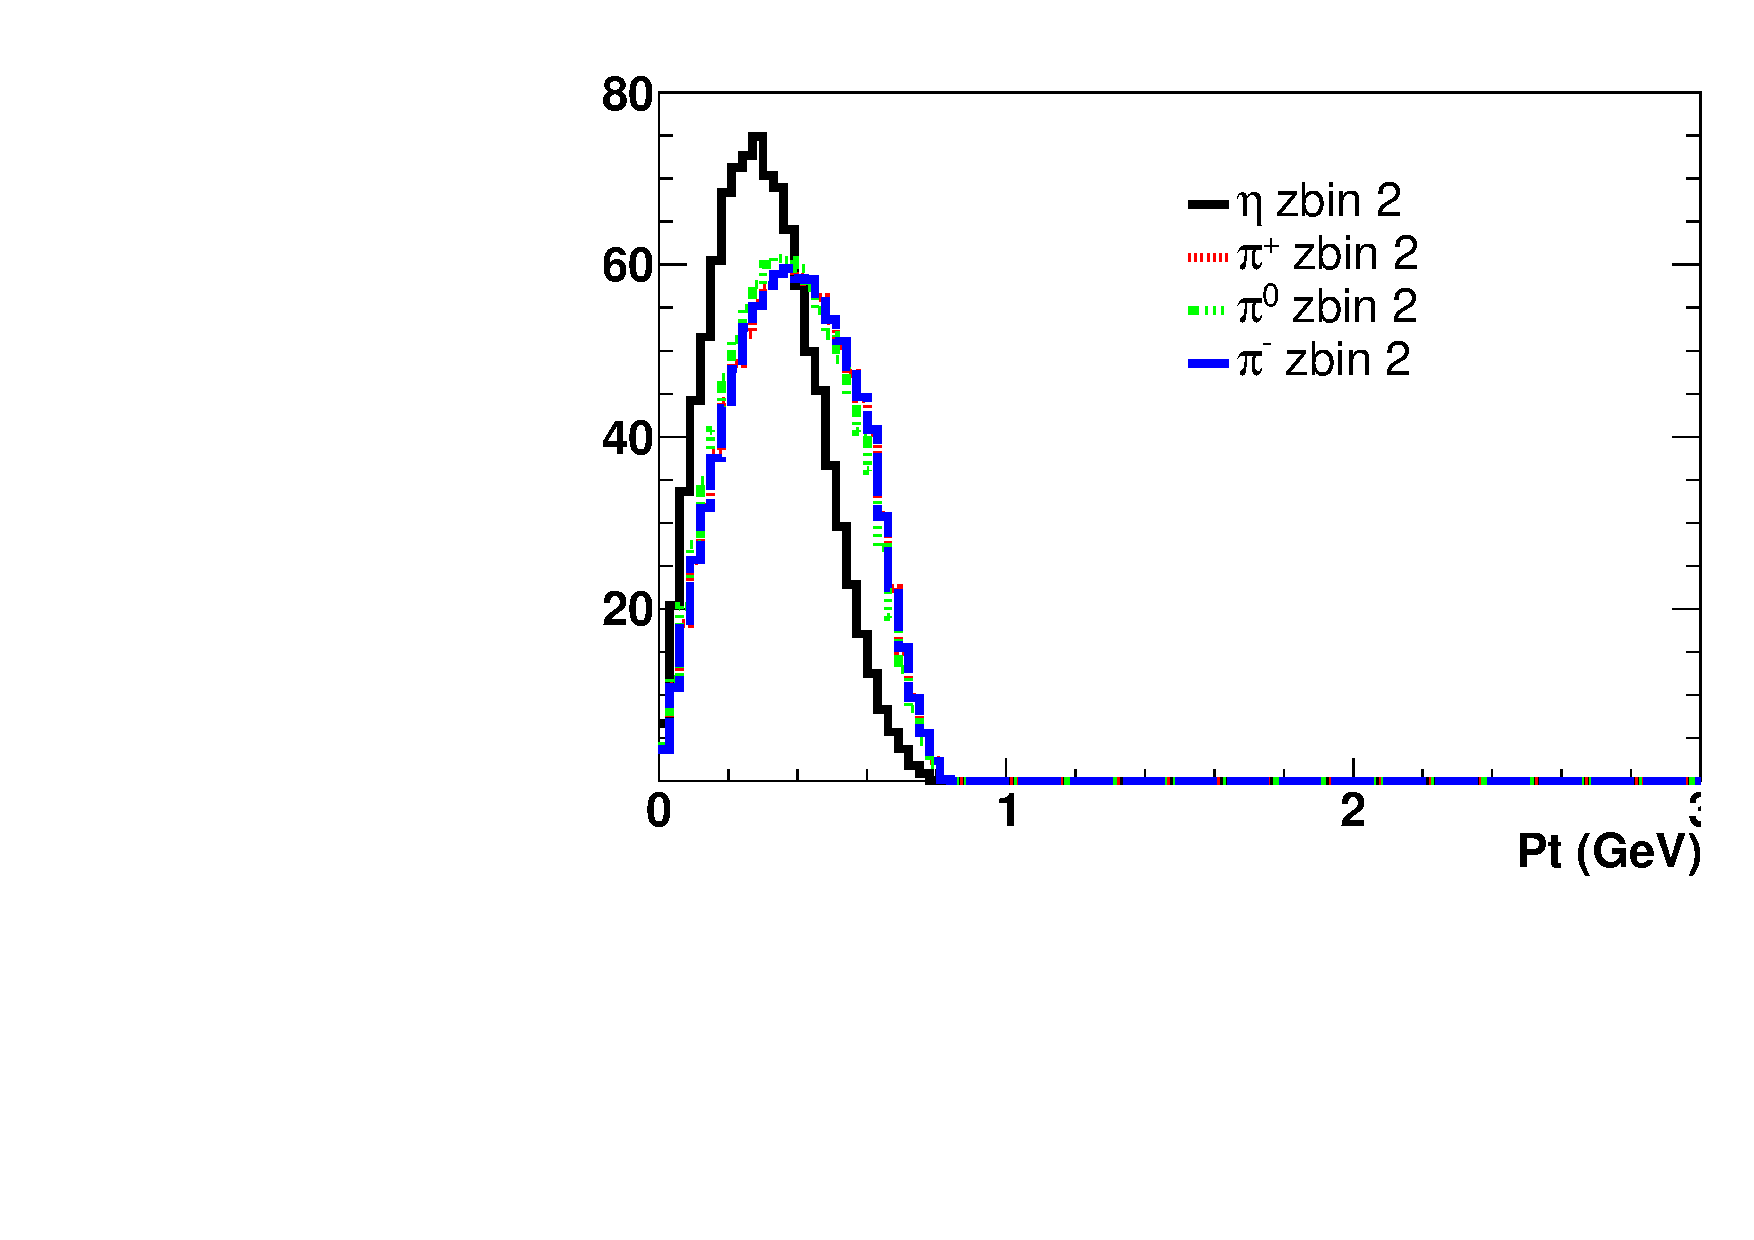
\includegraphics[width=.31\textwidth,natwidth=250,natheight=100]{figure_fiducial/had0.4_z0.3/Pt_distri_for_zbin_2_norm_had04z03.pdf}\label{fig:kine_distri52}}
\caption{Normalized $P_t$ distribution of $\eta$ and pions for $0.3<z<0.4$}
\label{fig:kine_distri5}
\end{figure}

\begin{figure}[H]
\captionsetup[subfloat]{farskip=2pt,captionskip=1pt}
\centering
\subfigure[$H_{OA}<0.3$]{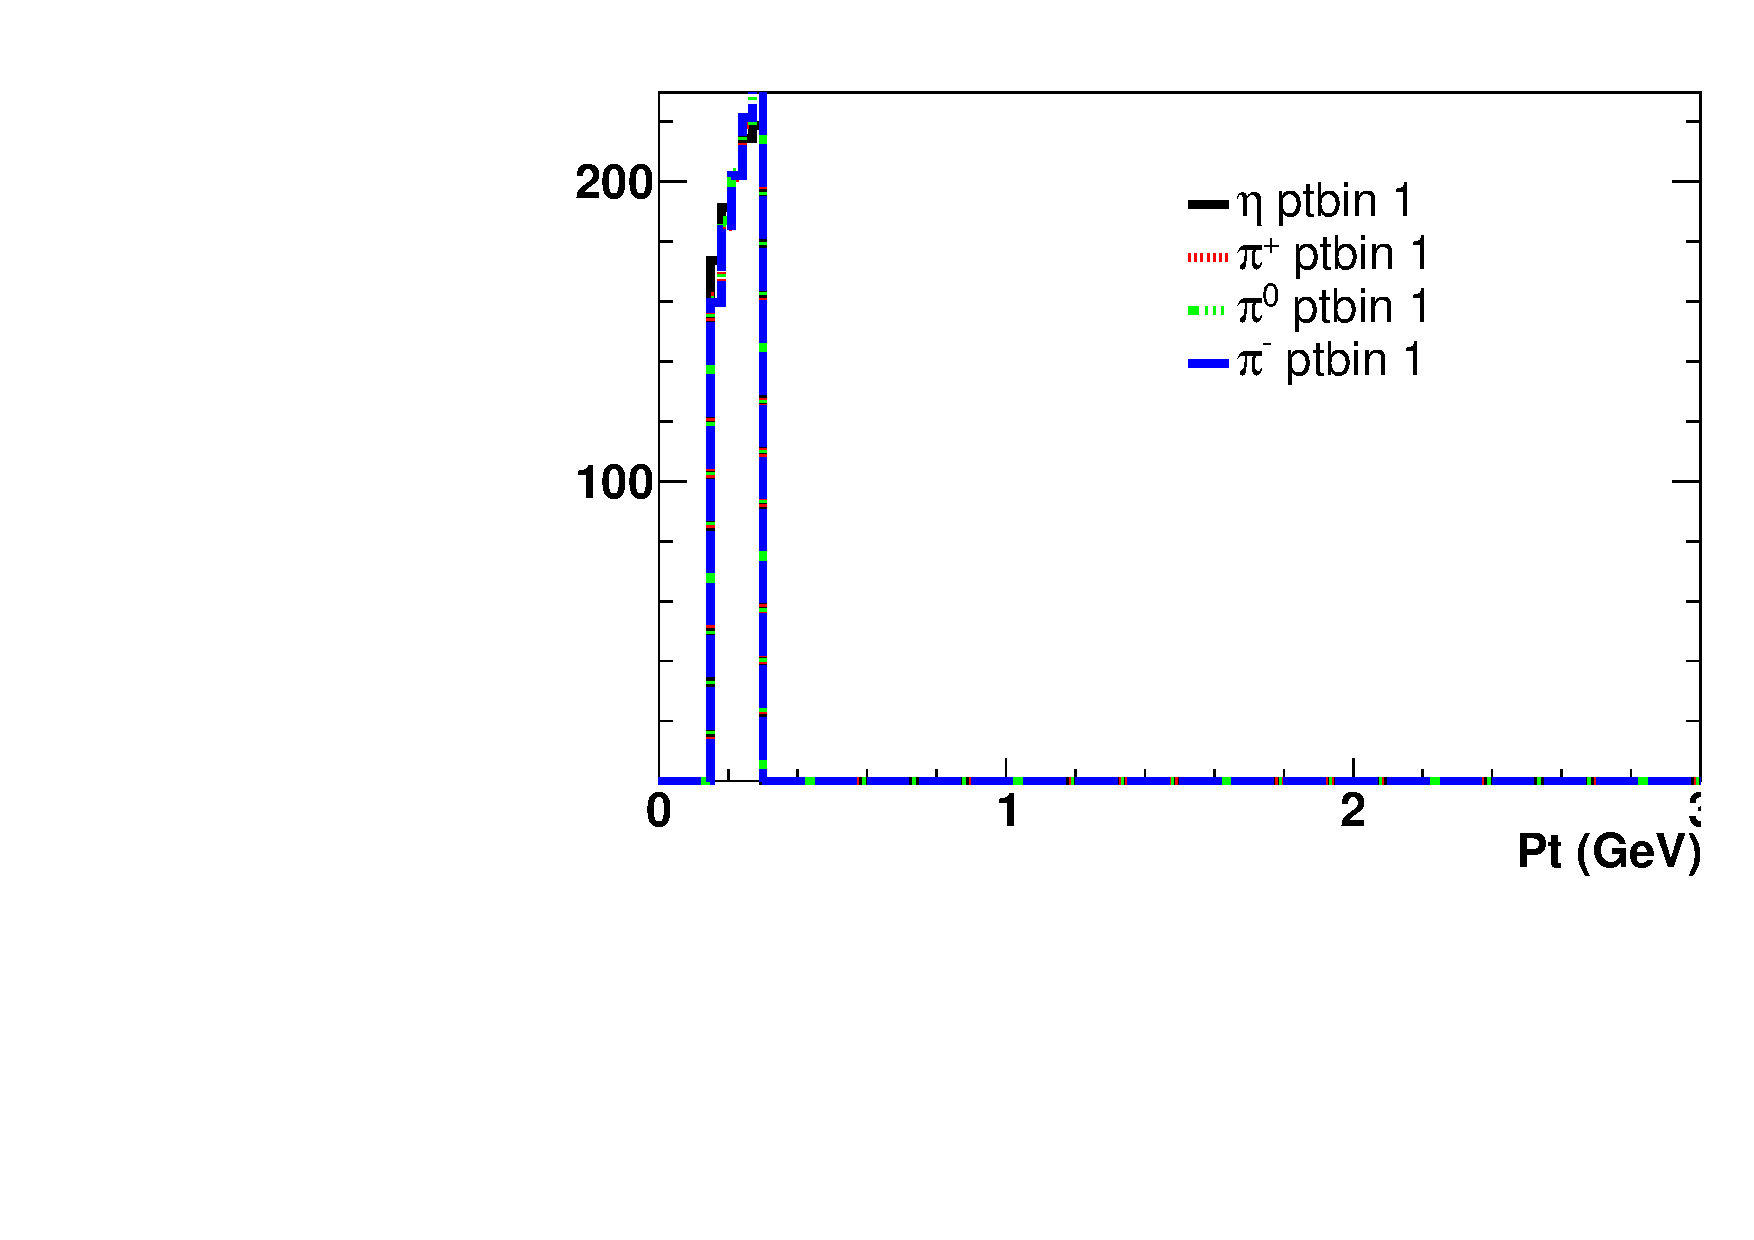
\includegraphics[width=.31\textwidth,natwidth=250,natheight=100]{figure_fiducial/had0.3_z0.3/Pt_distri_for_ptbin_1_norm_had03z03.pdf}\label{fig:kine_distri61}}
\subfigure[$H_{OA}<0.4$]{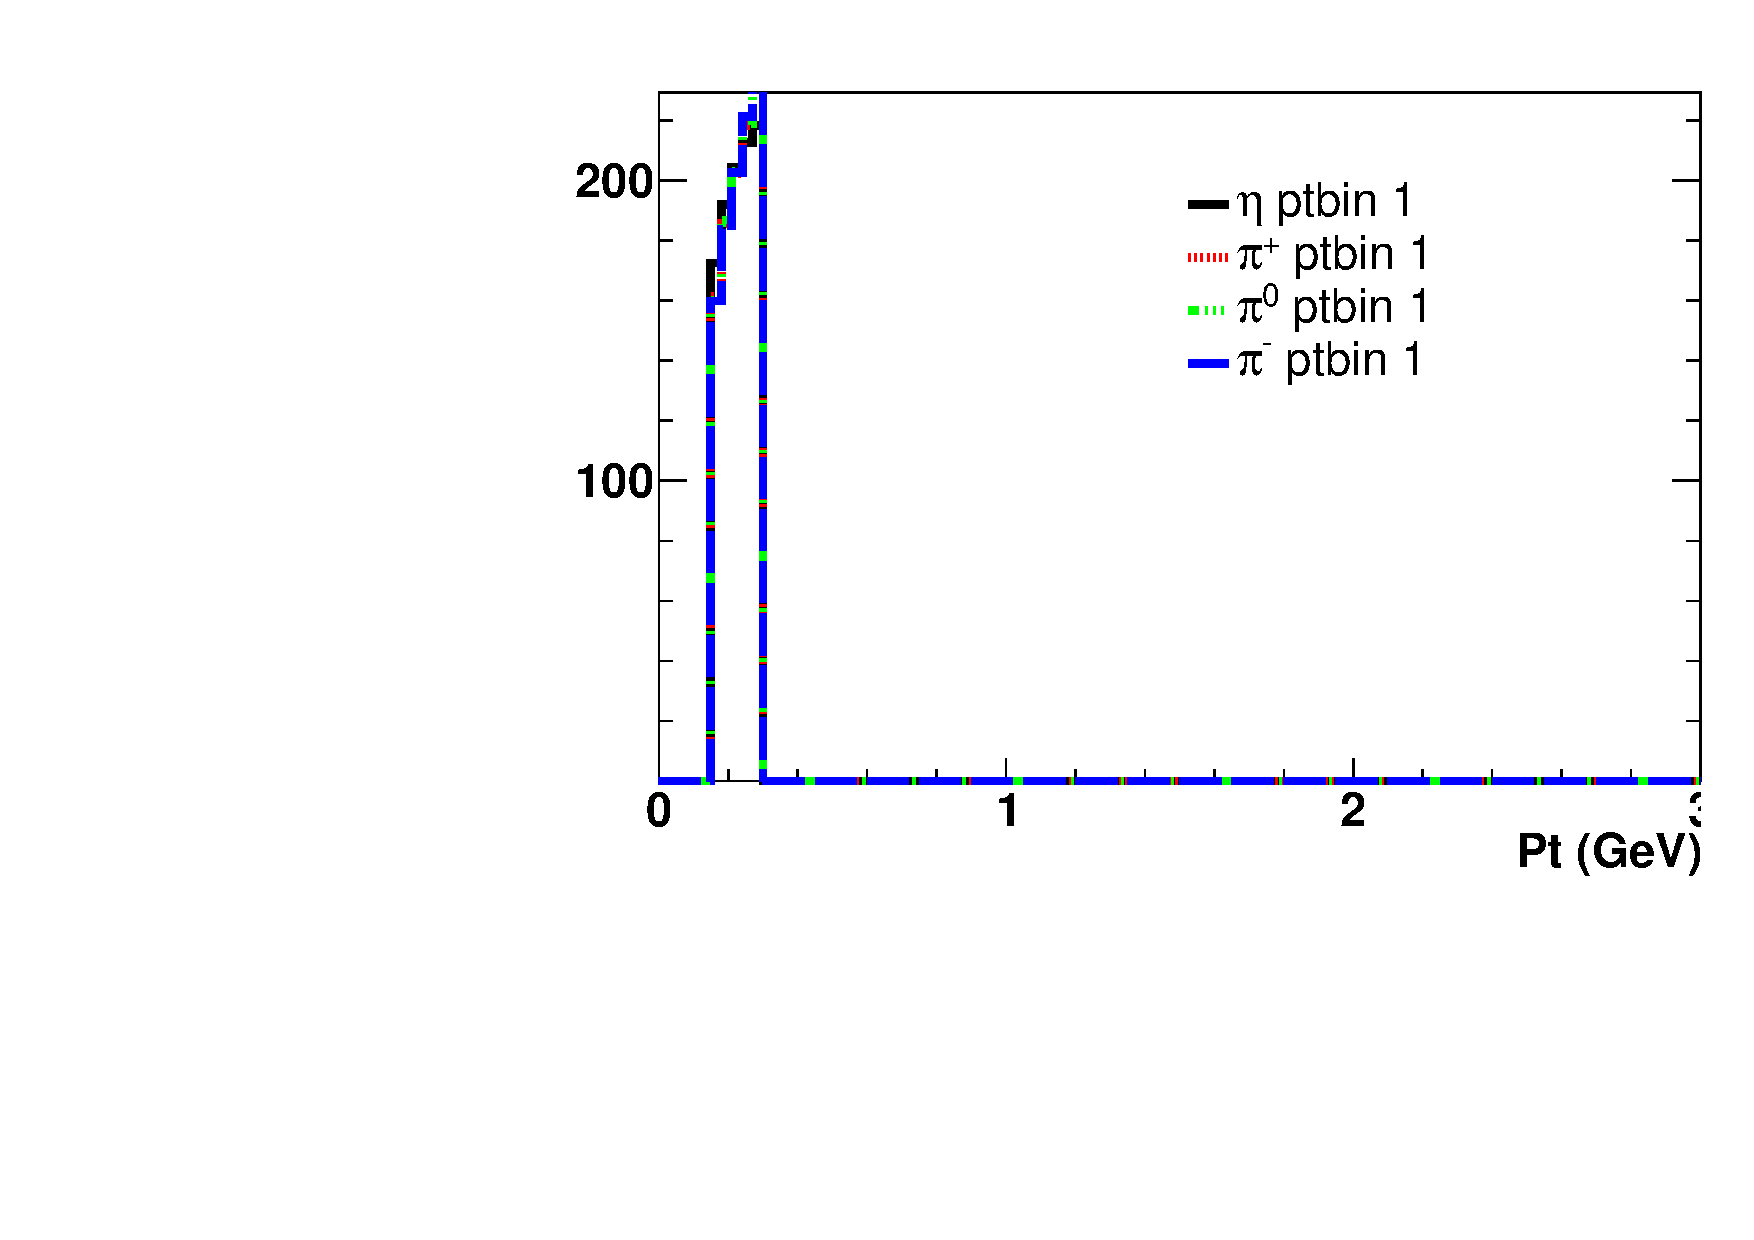
\includegraphics[width=.31\textwidth,natwidth=250,natheight=100]{figure_fiducial/had0.4_z0.3/Pt_distri_for_ptbin_1_norm_had04z03.pdf}\label{fig:kine_distri62}}
\caption{Normalized $P_t$ distribution of $\eta$ and pions for $0.15<P_t<0.3$}
\label{fig:kine_distri6}
\end{figure}

\begin{figure}[H]
\captionsetup[subfloat]{farskip=2pt,captionskip=1pt}
\centering
\subfigure[$H_{OA}<0.3$]{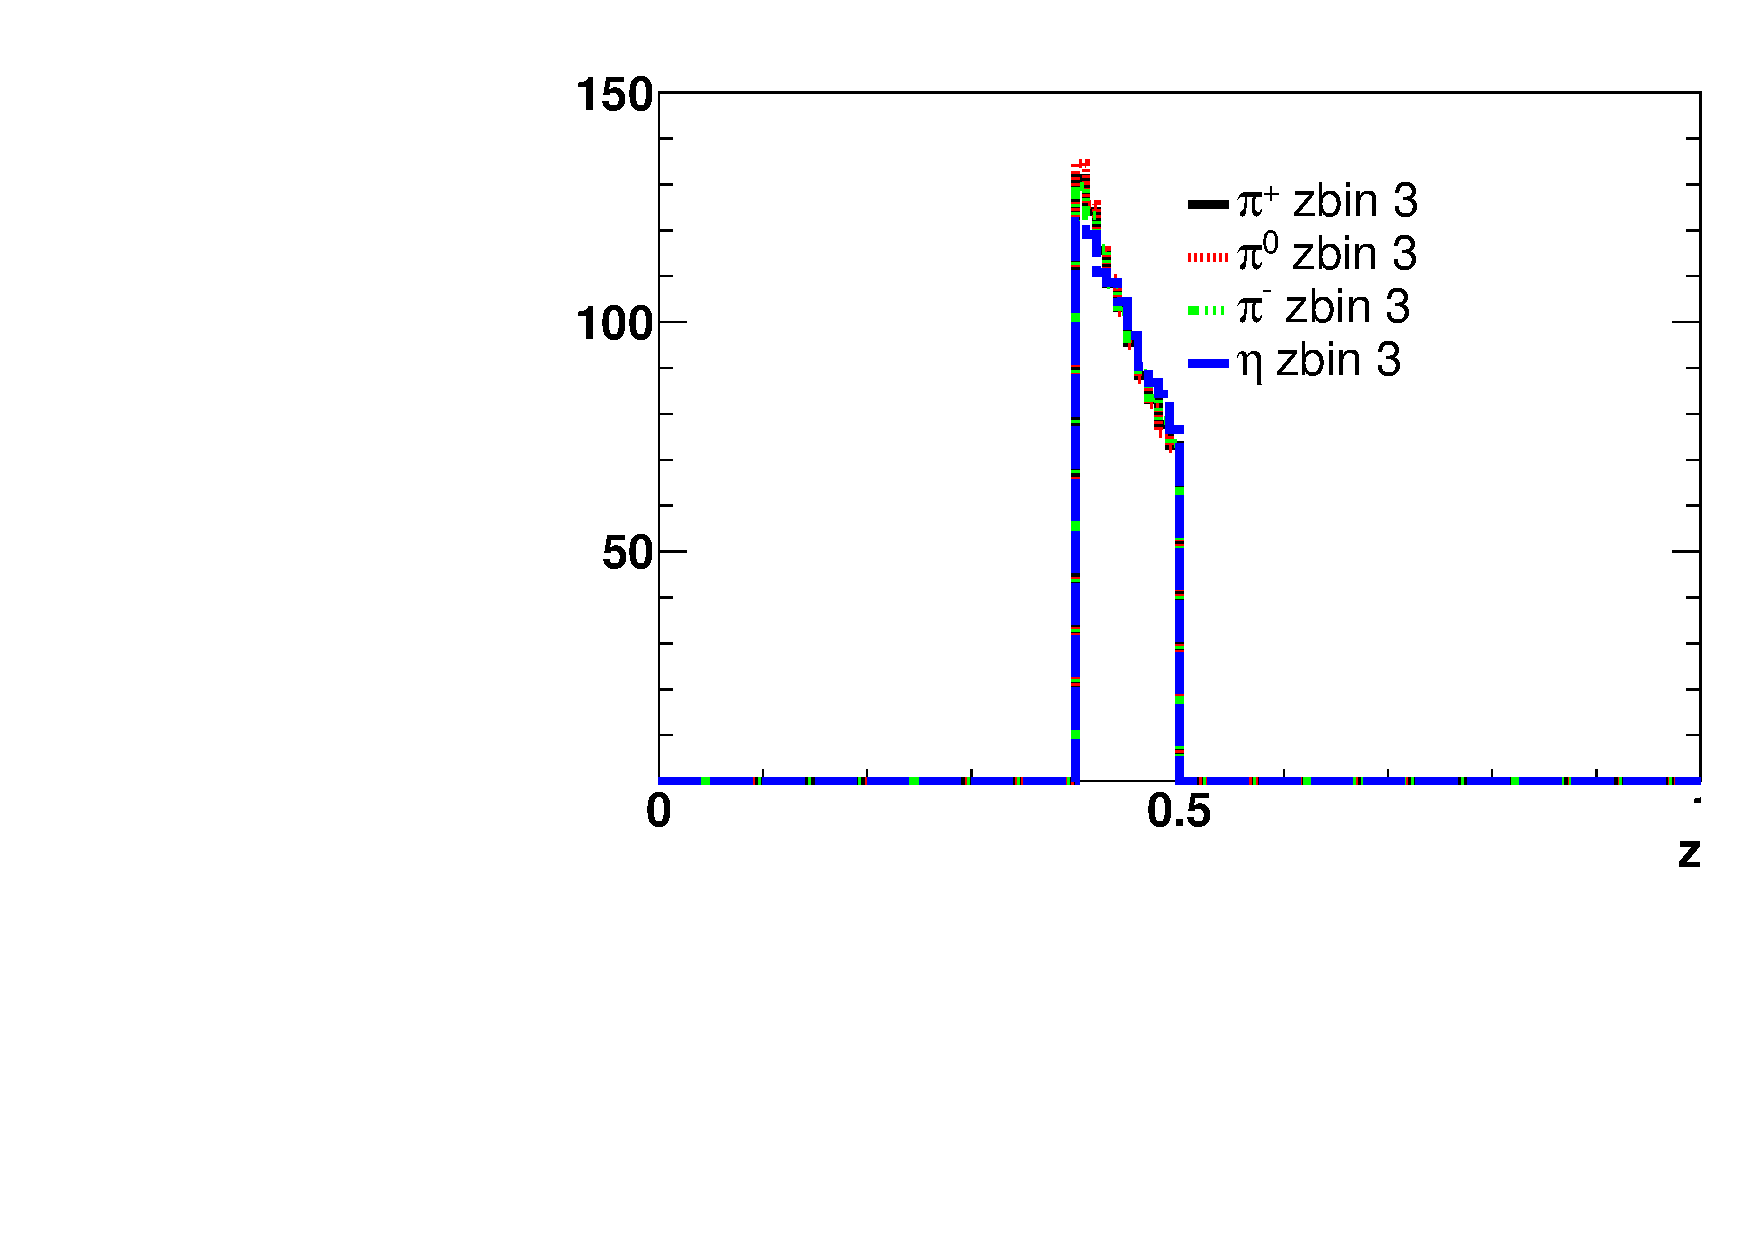
\includegraphics[width=.31\textwidth,natwidth=250,natheight=100]{figure_fiducial/had0.3_z0.3/Z_distri_for_zbin_3_norm_had03z03.pdf}\label{fig:kine_distri71}}
\subfigure[$H_{OA}<0.4$]{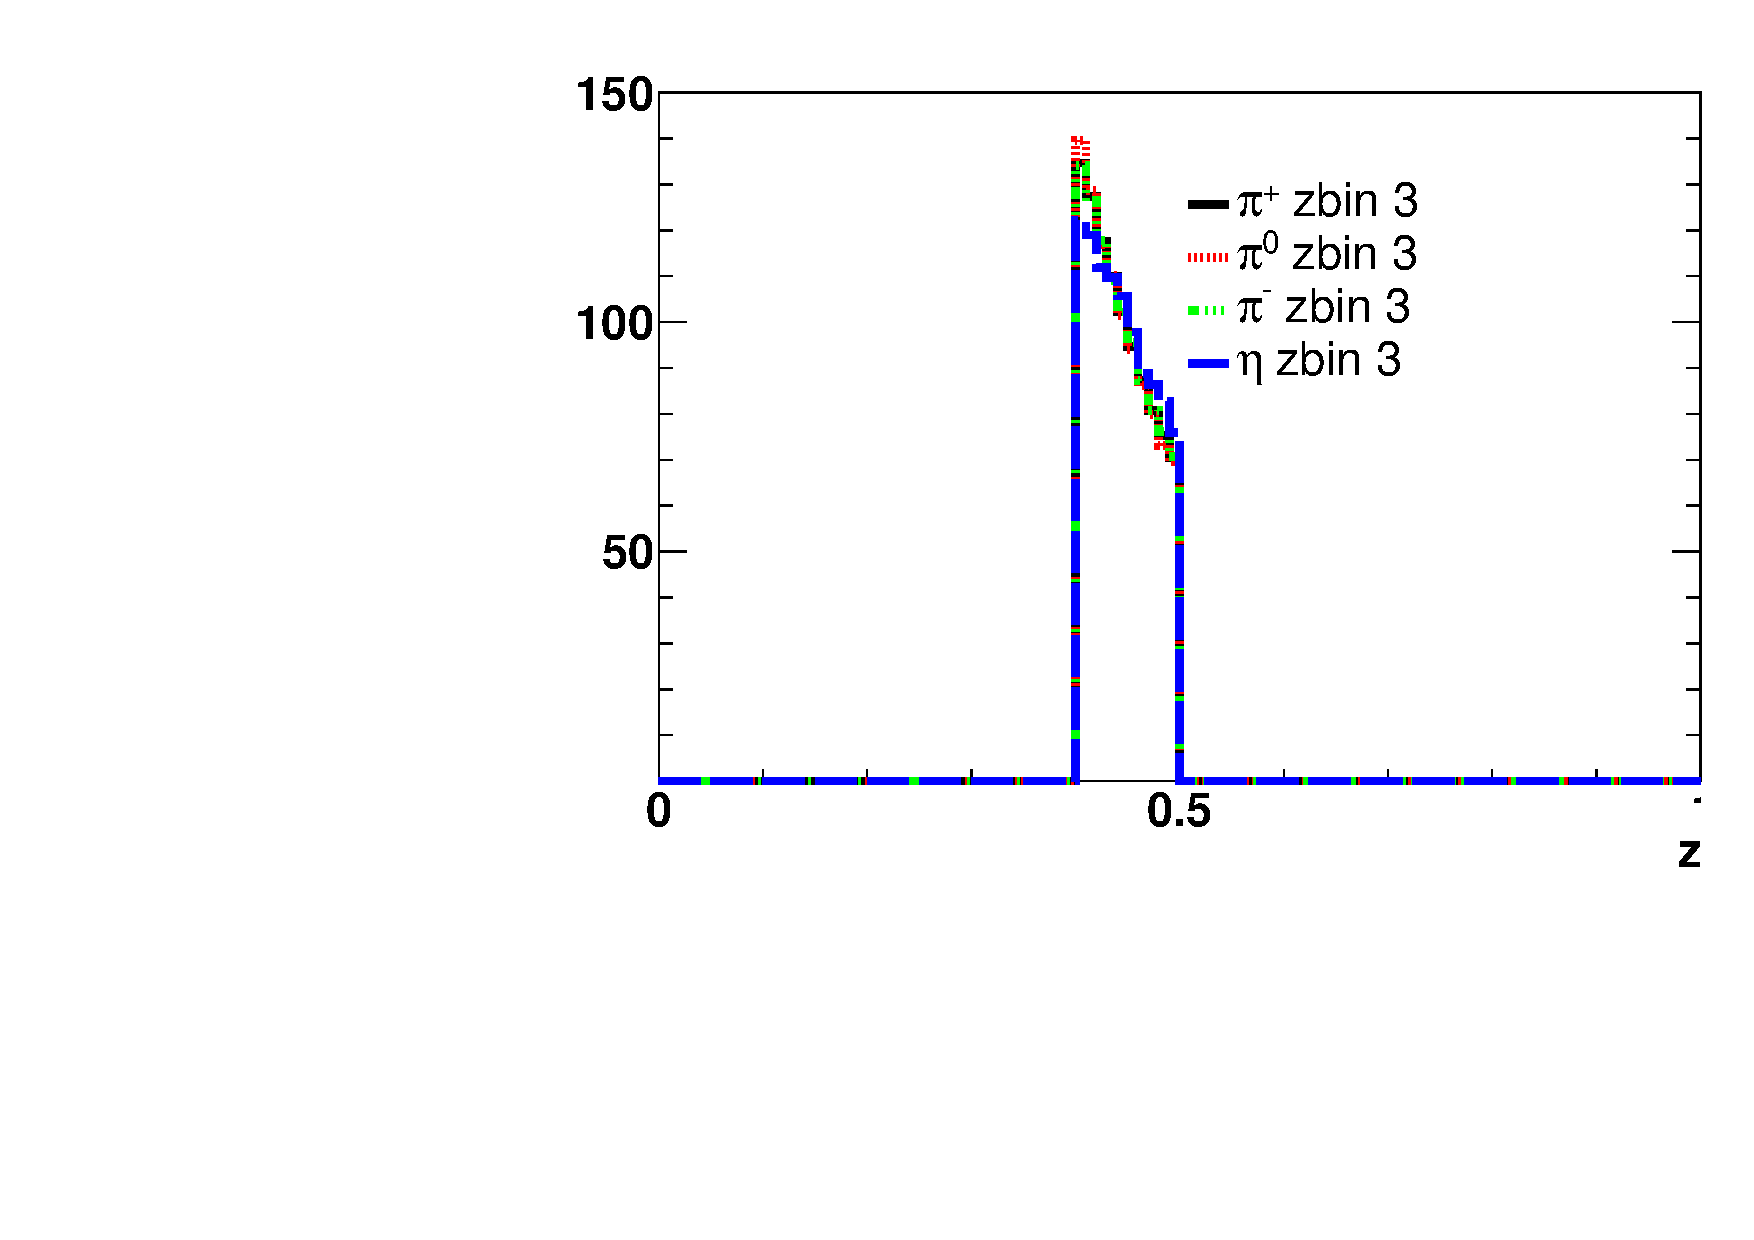
\includegraphics[width=.31\textwidth,natwidth=250,natheight=100]{figure_fiducial/had0.4_z0.3/Z_distri_for_zbin_3_norm_had04z03.pdf}\label{fig:kine_distri72}}
\caption{Normalized $z$ distribution of $\eta$ and pions for $0.4<z<0.5$}
\label{fig:kine_distri7}
\end{figure}

\begin{figure}[H]
\captionsetup[subfloat]{farskip=2pt,captionskip=1pt}
\centering
\subfigure[$H_{OA}<0.3$]{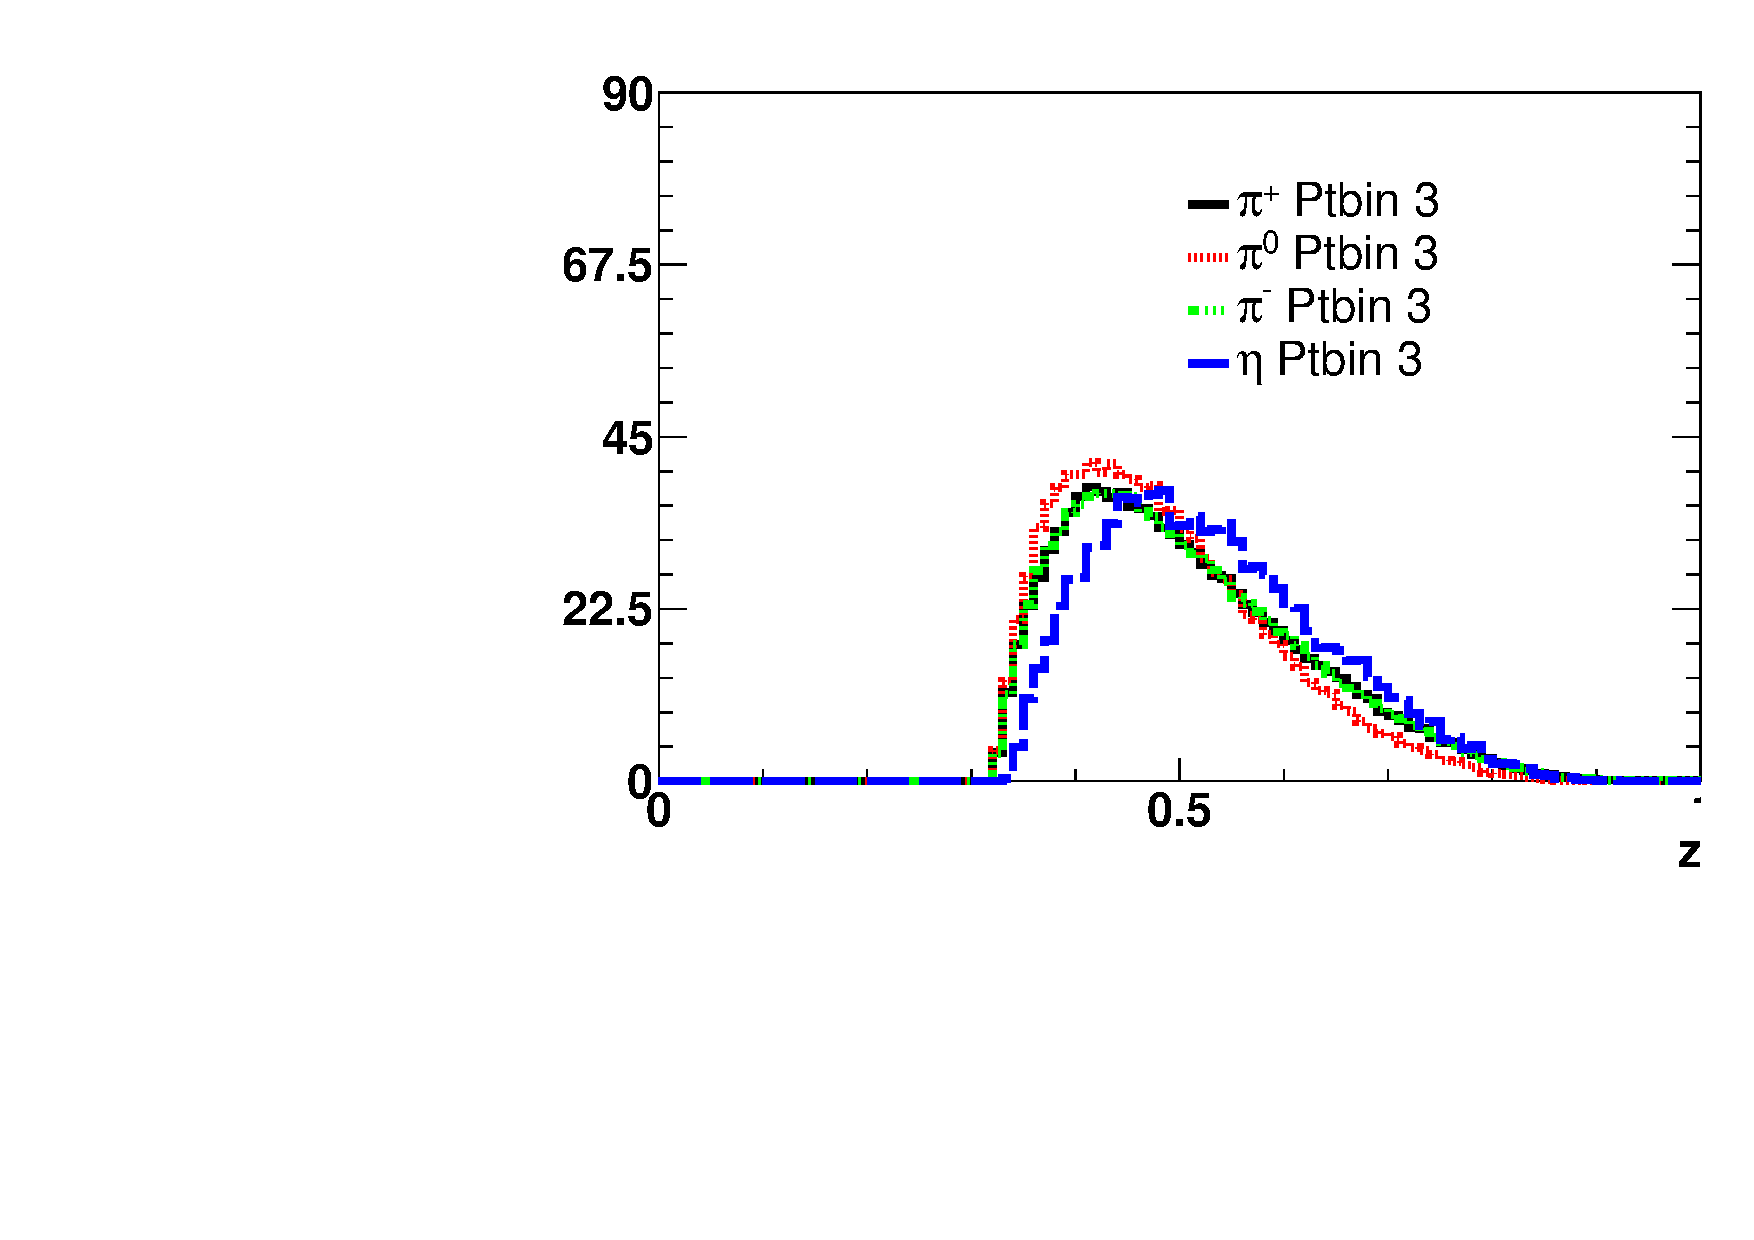
\includegraphics[width=.31\textwidth,natwidth=250,natheight=100]{figure_fiducial/had0.3_z0.3/Z_distri_for_ptbin_3_norm_had03z03.pdf}\label{fig:kine_distri81}}
\subfigure[$H_{OA}<0.4$]{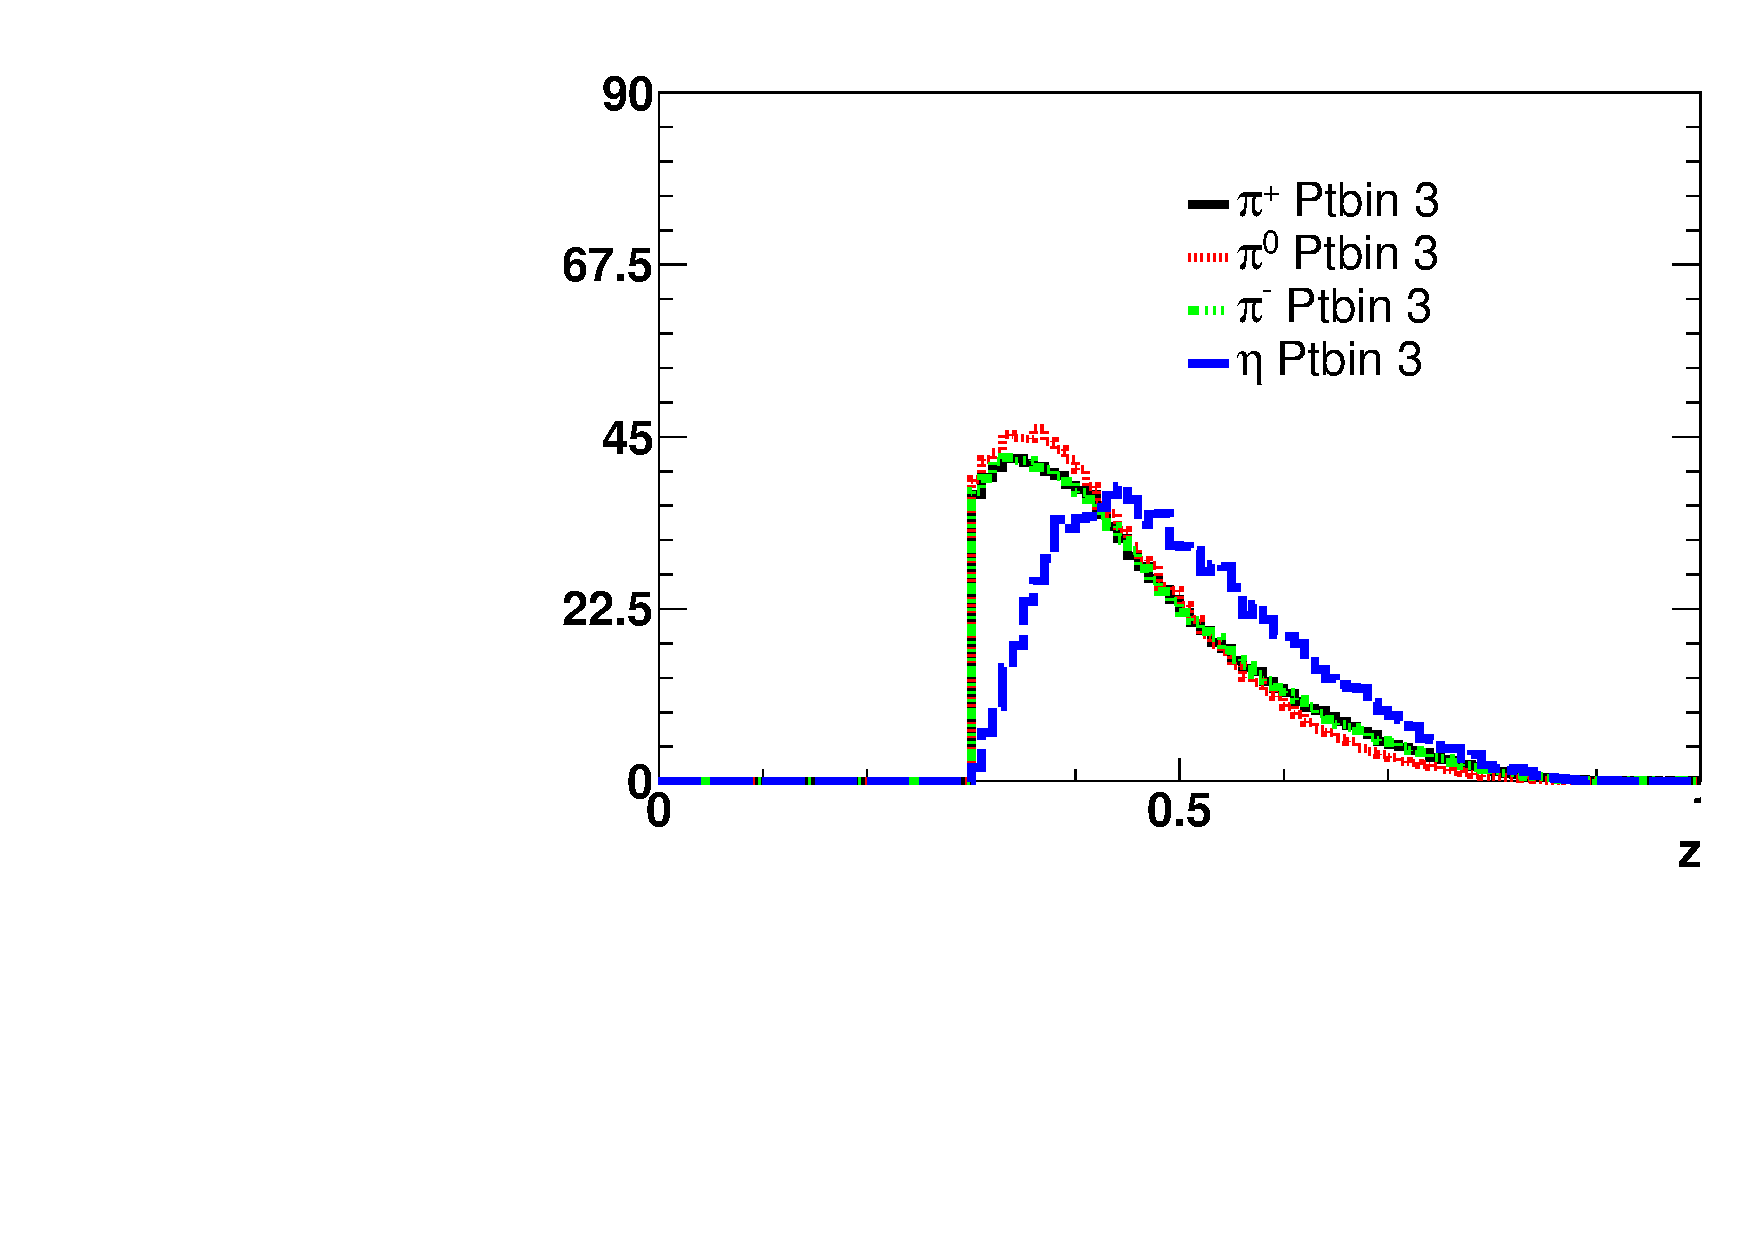
\includegraphics[width=.31\textwidth,natwidth=250,natheight=100]{figure_fiducial/had0.4_z0.3/Z_distri_for_ptbin_3_norm_had04z03.pdf}\label{fig:kine_distri82}}
\caption{Normalized $z$ distribution of $\eta$ and pions for $0.5<P_t<3$}
\label{fig:kine_distri8}
\end{figure}

By visually inspecting the above distributions, we choose the maximum value of hadron to thrust opening angle ($H_{OA}$) as $0.3$ to get matching hadron kinematics distributions. 



In summary, the principle behind the fiducial constraints summarized in Table~\ref{tab:constrain} is that all particles are captured by the barrel EMCAL, the hadrons are accepted symmetrically around the thrust axis and the acceptance for all hadrons is similar,  indicated by similar kinematic distributions. With $\gamma_{OA}<0.5$ we obtained the highest FOM: Accordingly $H_{OA}$ is set to 0.3 for all, i.e., charged and neutral, hadrons considered here, to satisfy the requirement of similar geometric acceptance. Fig.~\ref{fig:differentthetarange} compares the $\phi_1+\phi_2$ distribution for $\pi^0\pi^++\pi^0\pi^-$ pairs with and without applying the set of fiducial constraints. It can be seen that after applying the fiducial constraints, the amplitude of $R_{12}$ reduces significantly. This result also illustrates that  most of the false asymmetry comes from a detector effect since it can be removed by applying appropriate fiducial cuts. Last but not least, it should be noted that all these studies were performed on the Belle MC sample using PYTHIA $6.1$. The simulation does not contain the Collins effect, thus any remaing Collins-like $cos$ distribution originates from  the so-called false asymmetry arising from detector acceptance effects. 
\begin{figure}[h]
    \centering
    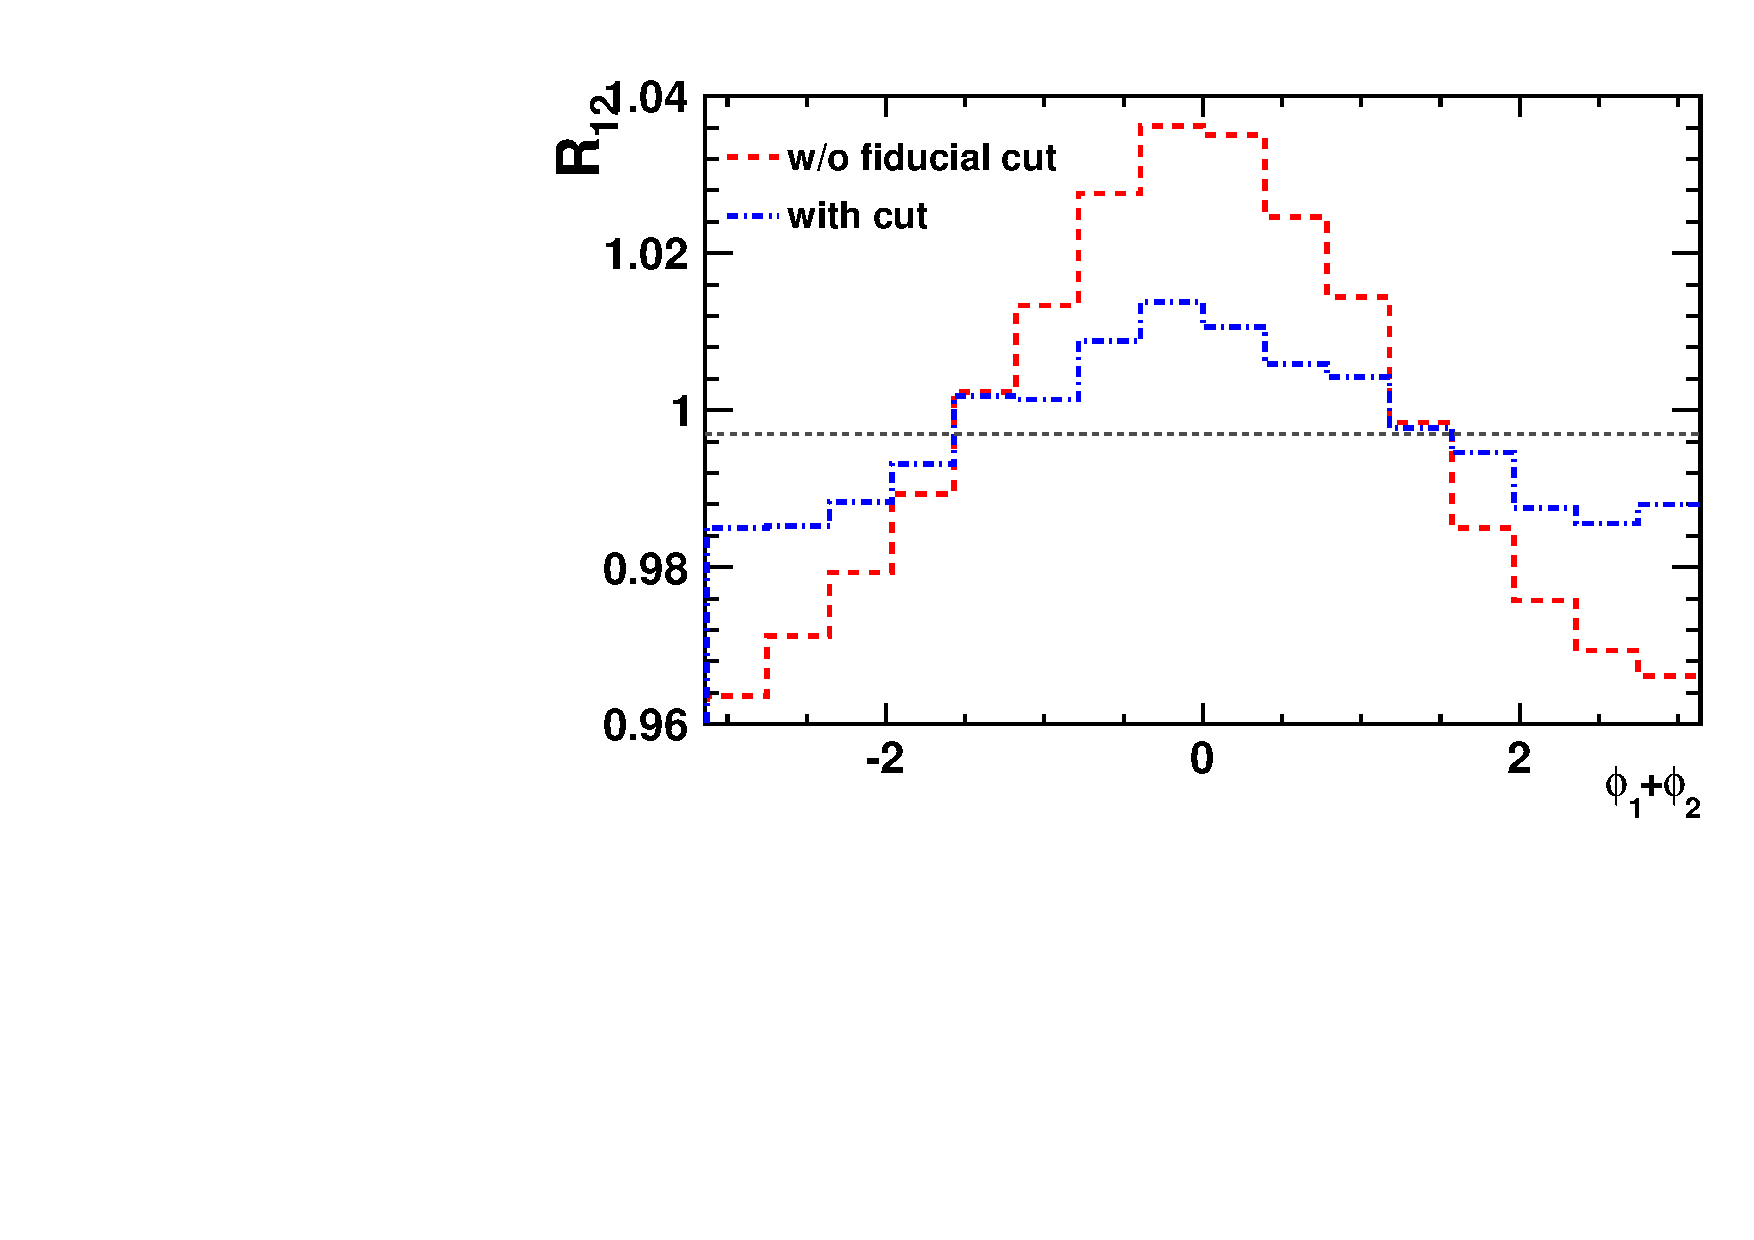
\includegraphics[width=0.8\textwidth,natwidth=610,natheight=642]{figure_dataselection/DetectorEffect.pdf}
    \caption{The normalized ratio $R_{12}$ for $\pi^0\pi^++\pi^0\pi^-$ with $0.3<z<0.4$ using MC data. The red histogram stands for the situation that no thrust or hadron direction cuts are applied. The blue histogram uses the criteria $\gamma_{OA} <0.3~\text{rad}$, $H_{OA}<0.5~\text{rad}$ and $1.34~\text{rad}<\theta<2.03~\text{rad}$.}
    \label{fig:differentthetarange}
\end{figure}


The final cuts on opening angle and photon energy are shown in Table~\ref{tab:constrain}. Note that the photon energy asymmetry cut is not listed since we determined that opening this cut optimizes the FOM.
%\begin{itemize}
%\item $\gamma$ energy constraint $50$~MeV for $\pi^0$, $150$~MeV for $\eta$.
%\item $z>0.1$ for hadrons forming double ratios that contain $\pi^0$.\footnote{For the kinematic bins where $z$ is  integrated, the threshold is increased to $z>0.2$. More details can be found in section~\ref{sec:kinematicbins}.}
%\item $z>0.3$ for hadrons forming double ratios that contain $\eta$, accounting for the higher $\eta$ mass and photon energy cut. 
%\end{itemize}

\begin{table}[H]\small
\centering
\begin{tabular}{|l|l|l|l|l|l|l|l|l|}
\hline
constraints & cut   \\ \hline
$E_\gamma$~($\pi^0$) & $E_\gamma >50$~MeV \\ \hline
$E_\gamma$~($\eta$) & $E_\gamma >250$~MeV \\ \hline
$z$  for hadrons forming double ratios &\multirow{2}{*}{$z>0.1$}\\
 that contain $\pi^0$.\footnote{For the kinematic bins where $z$ is  integrated, the threshold is increased to $z>0.2$. More details can be found in section~\ref{sec:kinematicbins}.}&  \\ \hline
$z$ for hadrons forming double ratios that contain $\eta$,& \multirow{3}{*}{$z>0.3$} \\ accounting for the higher $\eta$ mass &\\and photon energy cut. \\ \hline
$\gamma_{OA}$ (modulo $\pi$) & $<0.5$ \\ \hline
$H_{OA}$ (modulo $\pi$) & $<0.3$ \\ \hline
$\theta$ &  $1.34~\text{rad}$\textup{--}$ 2.03~\text{rad}$ \\ \hline
\end{tabular}
\caption{Fiducial and energy constraints for $\pi^0$ and $\eta$.}
\label{tab:constrain}
\end{table}

\subsection{Neutral Meson Reconstruction}
\label{sec:neutralmesonreconstruction}
This section discusses the reconstruction of the neutral mesons. In particular we discuss different fitting techniques to the two photon invariant mass spectrum to extract the $\pi^0$ yield in Sec.~\ref{sec:pi0fitsection}-\ref{sec:fit_with_MC_BG} and the fits to extract the $\eta$ yield in Sec.~\ref{sec:etafitsection}. Finally, we optimize the mass windows for the neutral meson extractions in Sec.~\ref{sec:masswindow}. The input to the fits described in this section are photon pairs that fulfill the energy and energy-asymmetry constrains outlined in the previous Sec.~\ref{sec:fidAndEnergyCuts}. 
These cuts suppress background from detector noise as well as combinatorial background.

\subsubsection{\texorpdfstring{Invariant Mass fit of $\pi^0$}{pi0 fit}}
\label{sec:pi0fitsection}
A reasonably good fit to the $\pi^0$ invariant mass spectrum can be achieved by using a polynomial function for the background and a Gaussian for the signal. However, we observed that our signal has large tails at low $m_{\pi^0}$. From simulation we could determine the reason. If a photon splits via  $\gamma\rightarrow e^+e^-$, one of the leptons can be lost, while the other is initiating a electromagnetic shower in the EMCAL and thus gets mistaken for a photon.
 Therefore, we decided to use the Crystal Ball function to fit the signal, since it can accommodate the observed asymmetric tails.  This fit is described in~\ref{sec:crystalBallFit}.
 It is also possible to extract the $\pi^0$ yield via a nonparametric method. For this we estimate the background shape from the simulation in the sidebands, extrapolate into the signal region, and subtract the background to extract the signal.  This fitting method is described in~\ref{sec:fit_with_MC_BG}.
For the final results we use the Crystal Ball fit and take the discrepancy of those two fitting methods as a source of systematic uncertainty.

\subsubsection{Fit with the Crystal Ball Function}
\label{sec:crystalBallFit}
We use a polynomial function of degree 5 and Crystal Ball function to describe the background and signal. The Crystal Ball function of $x$ is defined as~\cite{CrystalBallFunc}
\begin{subequations}
\begin{align}
f(x;\alpha,n,\bar x,\sigma) & = N \cdot \begin{cases} \exp(- \frac{(x - \bar x)^2}{2 \sigma^2}), & \mbox{for }\frac{x - \bar x}{\sigma} > -\alpha \\
 A \cdot (B - \frac{x - \bar x}{\sigma})^{-n}, & \mbox{for }\frac{x - \bar x}{\sigma} \leqslant -\alpha \end{cases}\\
A & = \left(\frac{n}{\left| \alpha \right|}\right)^n \cdot \exp\left(- \frac {\left| \alpha \right|^2}{2}\right), \\
B &= \frac{n}{\left| \alpha \right|}  - \left| \alpha \right|,\\
%N &=\frac{1}{\sigma(C+D)},
%C &=\frac{n}{\left|\alpha \right| \cdot \frac{1}{n-1} \cdot \exp(-\frac{\left| \alpha \right|^2}{2}),\\
%D &=\sqrt{\frac{\pi}{2}}(1+\DeclareMathOperator\erf{erf}(\frac{\left| \alpha \right|}{\sqrt{2}}))
N &= \frac{1}{\sigma (C + D)}\\
C &= \frac{n}{\left| \alpha \right|} \cdot \frac{1}{n-1} \cdot \exp\left(- \frac {\left| \alpha \right|^2}{2}\right) \\
D &= \sqrt{\frac{\pi}{2}} \left(1 + \operatorname{erf}\left(\frac{\left| \alpha \right|}{\sqrt 2}\right)\right) \\
\end{align}
\label{eqn:crystalball}
\end{subequations}
%Here the parameters $\sigma$ and $\bar x$ control the shape of the function similarly to the width and mean of a Gaussian. 
Figure~\ref{fig:pi0_crystalfit} contains some fitting examples. More plots can be found in Appendix~\ref{sec:cryfitpi0}. 
%min=0.055,max=0.22 
  The vertical black dash lines in the plots are boundaries of the signal mass window that we will discuss in section~\ref{sec:masswindow}. The fitting result (blue line) shows good agreement with experimental data except some slight differences in sideband regions. 
\begin{figure}[H]
  \centering     
  \subfigure[$\pi^0$ invariant mass fit, $0<P_t<0.15$]{\label{fig:pi0crystalfit_1}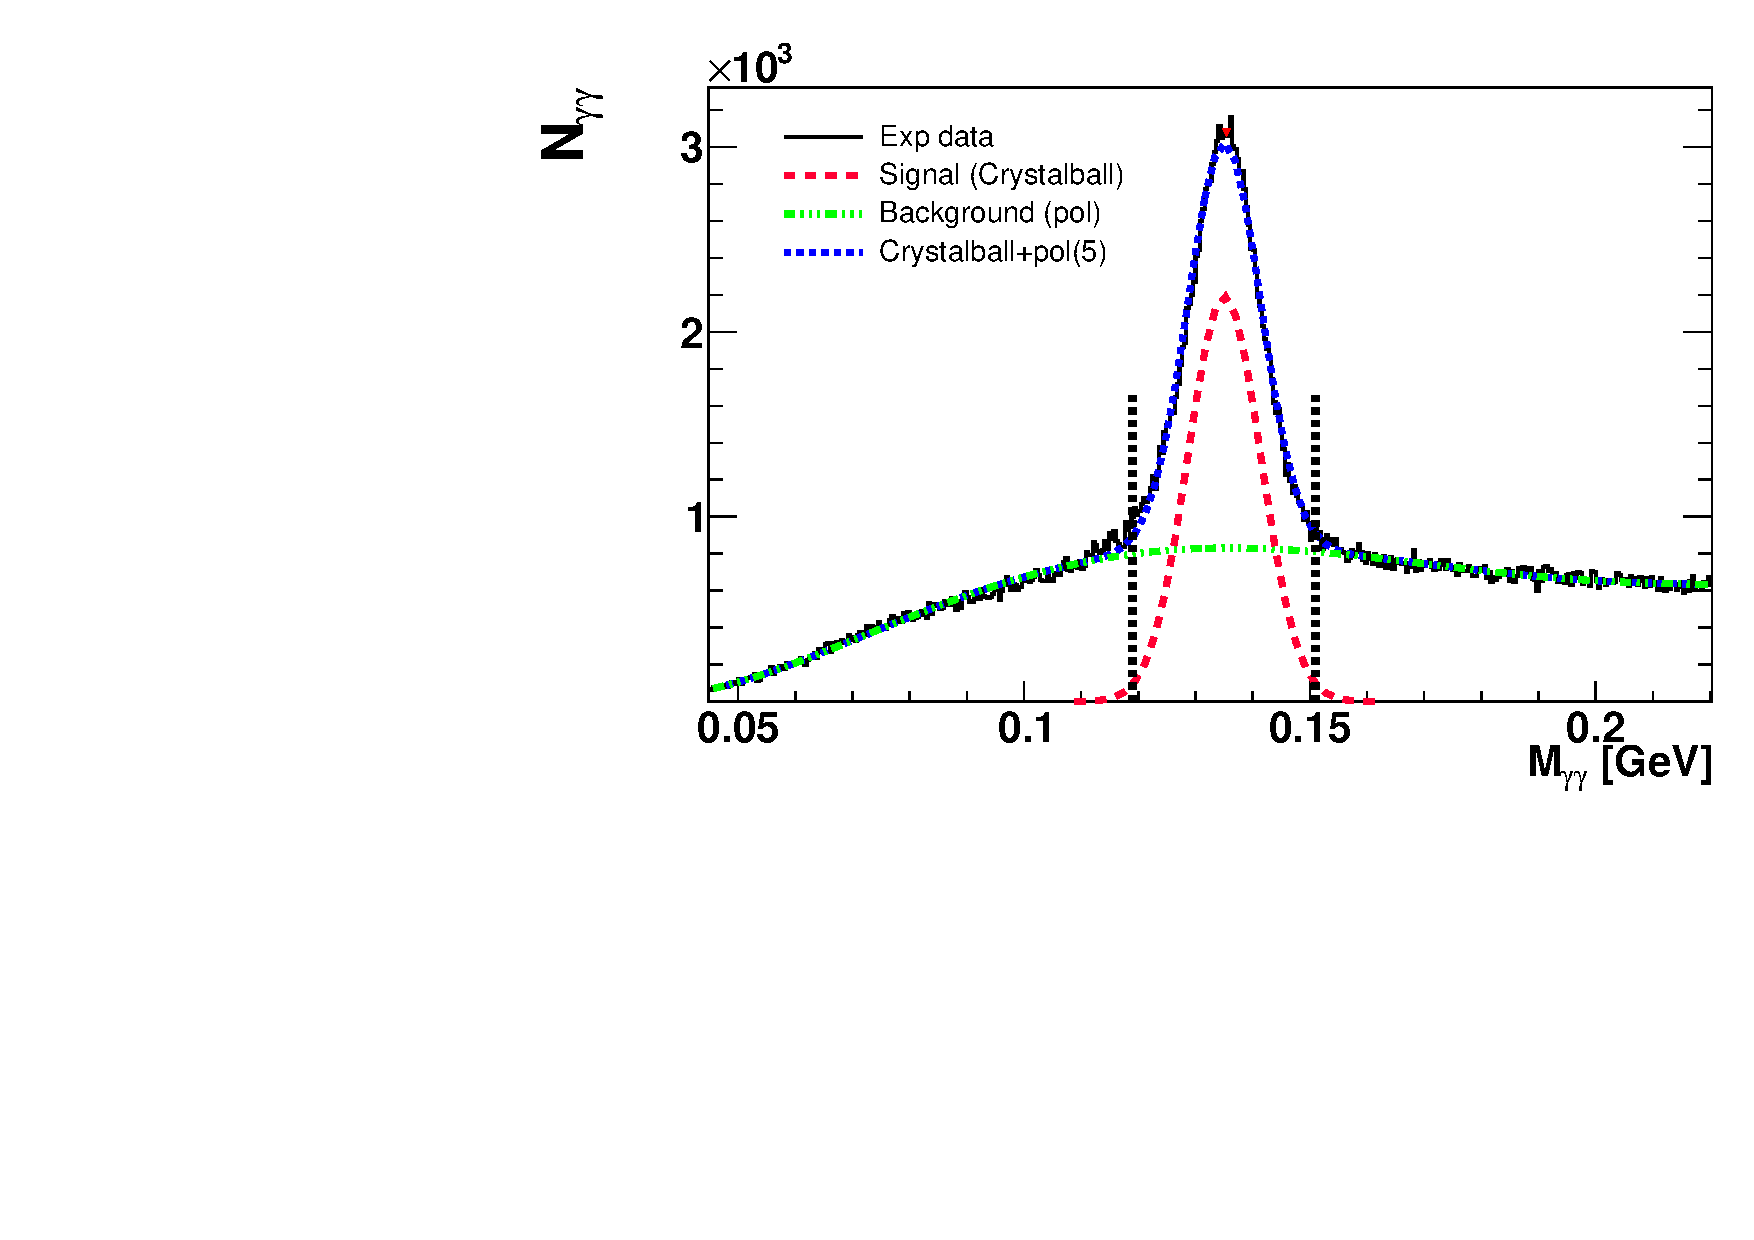
\includegraphics[width=.48\textwidth,natwidth=600,natheight=400]{figure_dataselection/pi0_crystalfit_Pt_0.pdf}}
  \subfigure[$\pi^0$ invariant mass fit, $0.3<P_t<0.5$]{\label{fig:pi0crystalfit_2}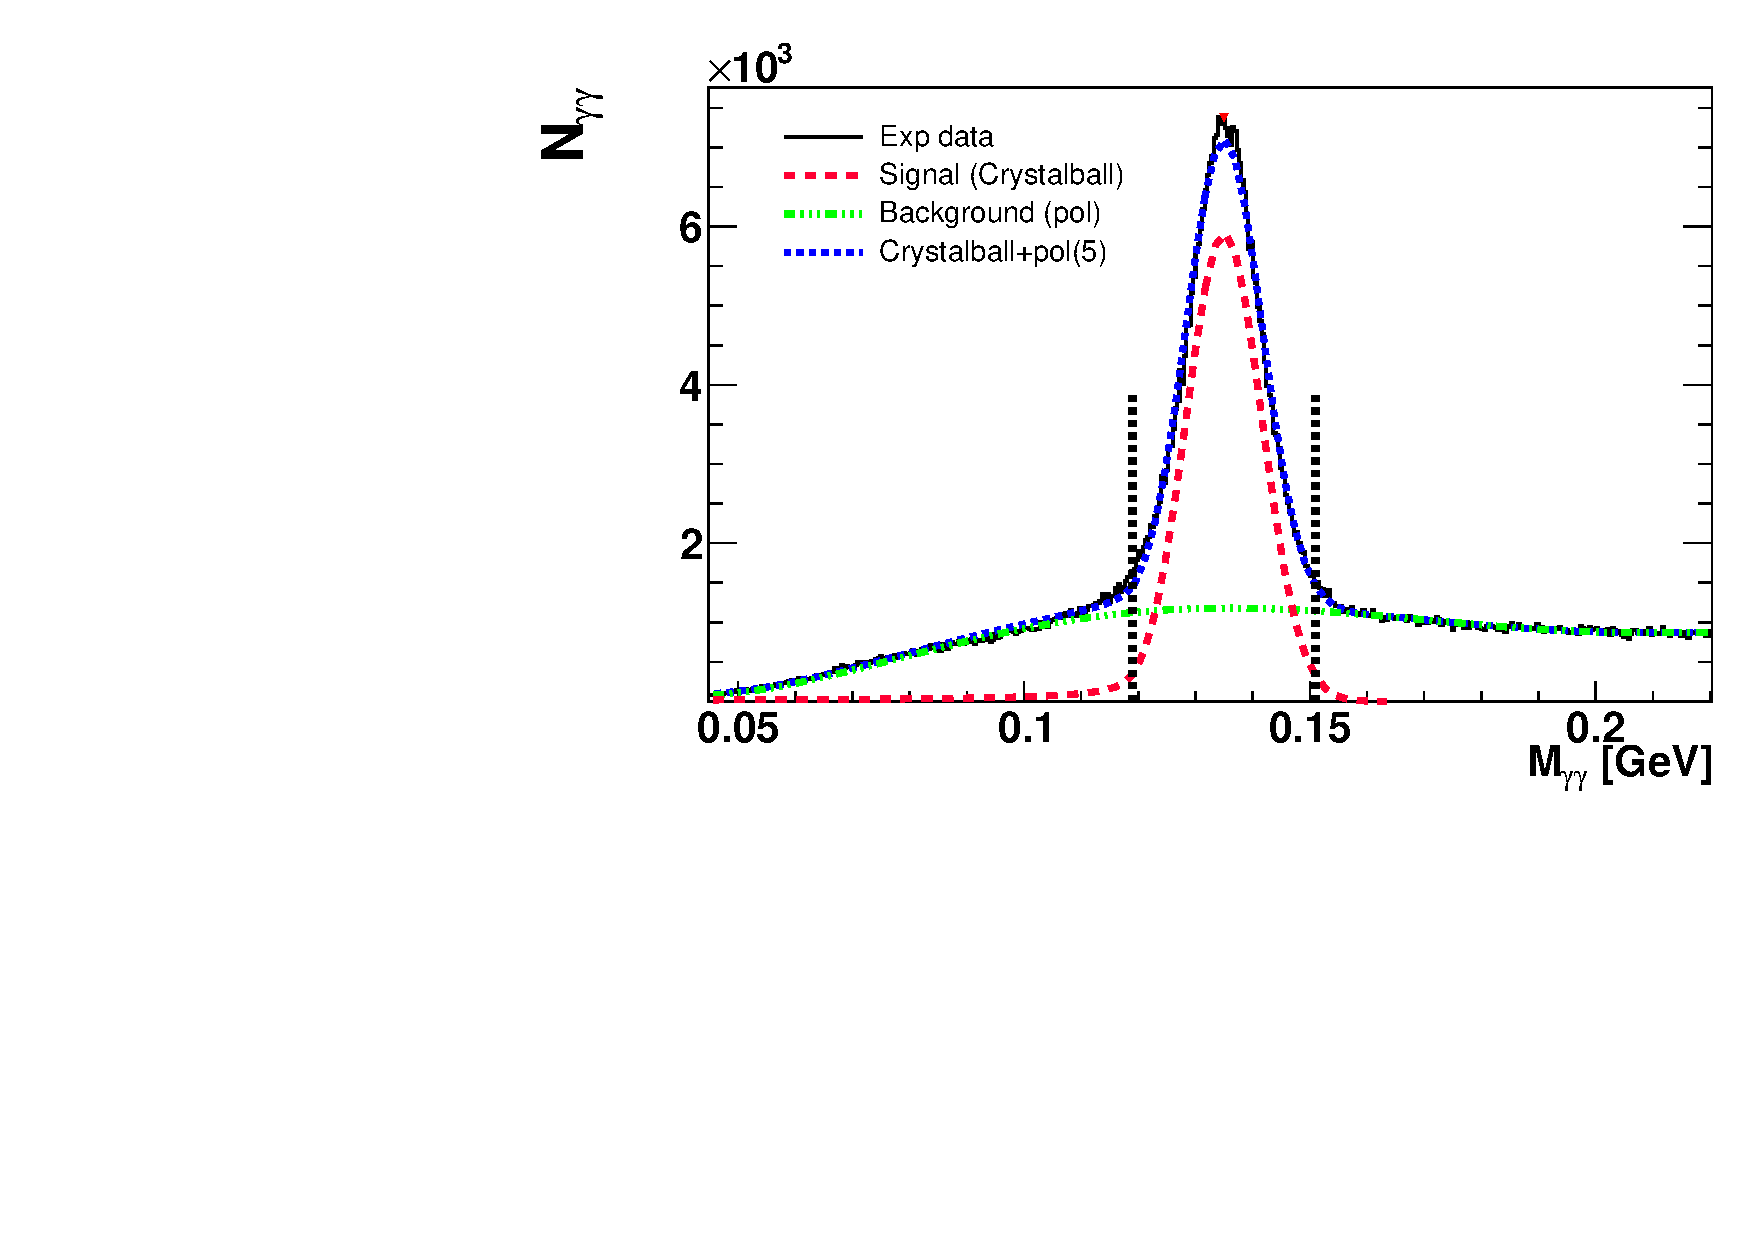
\includegraphics[width=.48\textwidth,natwidth=600,natheight=400]{figure_dataselection/pi0_crystalfit_Pt_2.pdf}}
  \subfigure[$\pi^0$ invariant mass fit, $0.2<z<0.3$]{\label{fig:pi0crystalfit_3}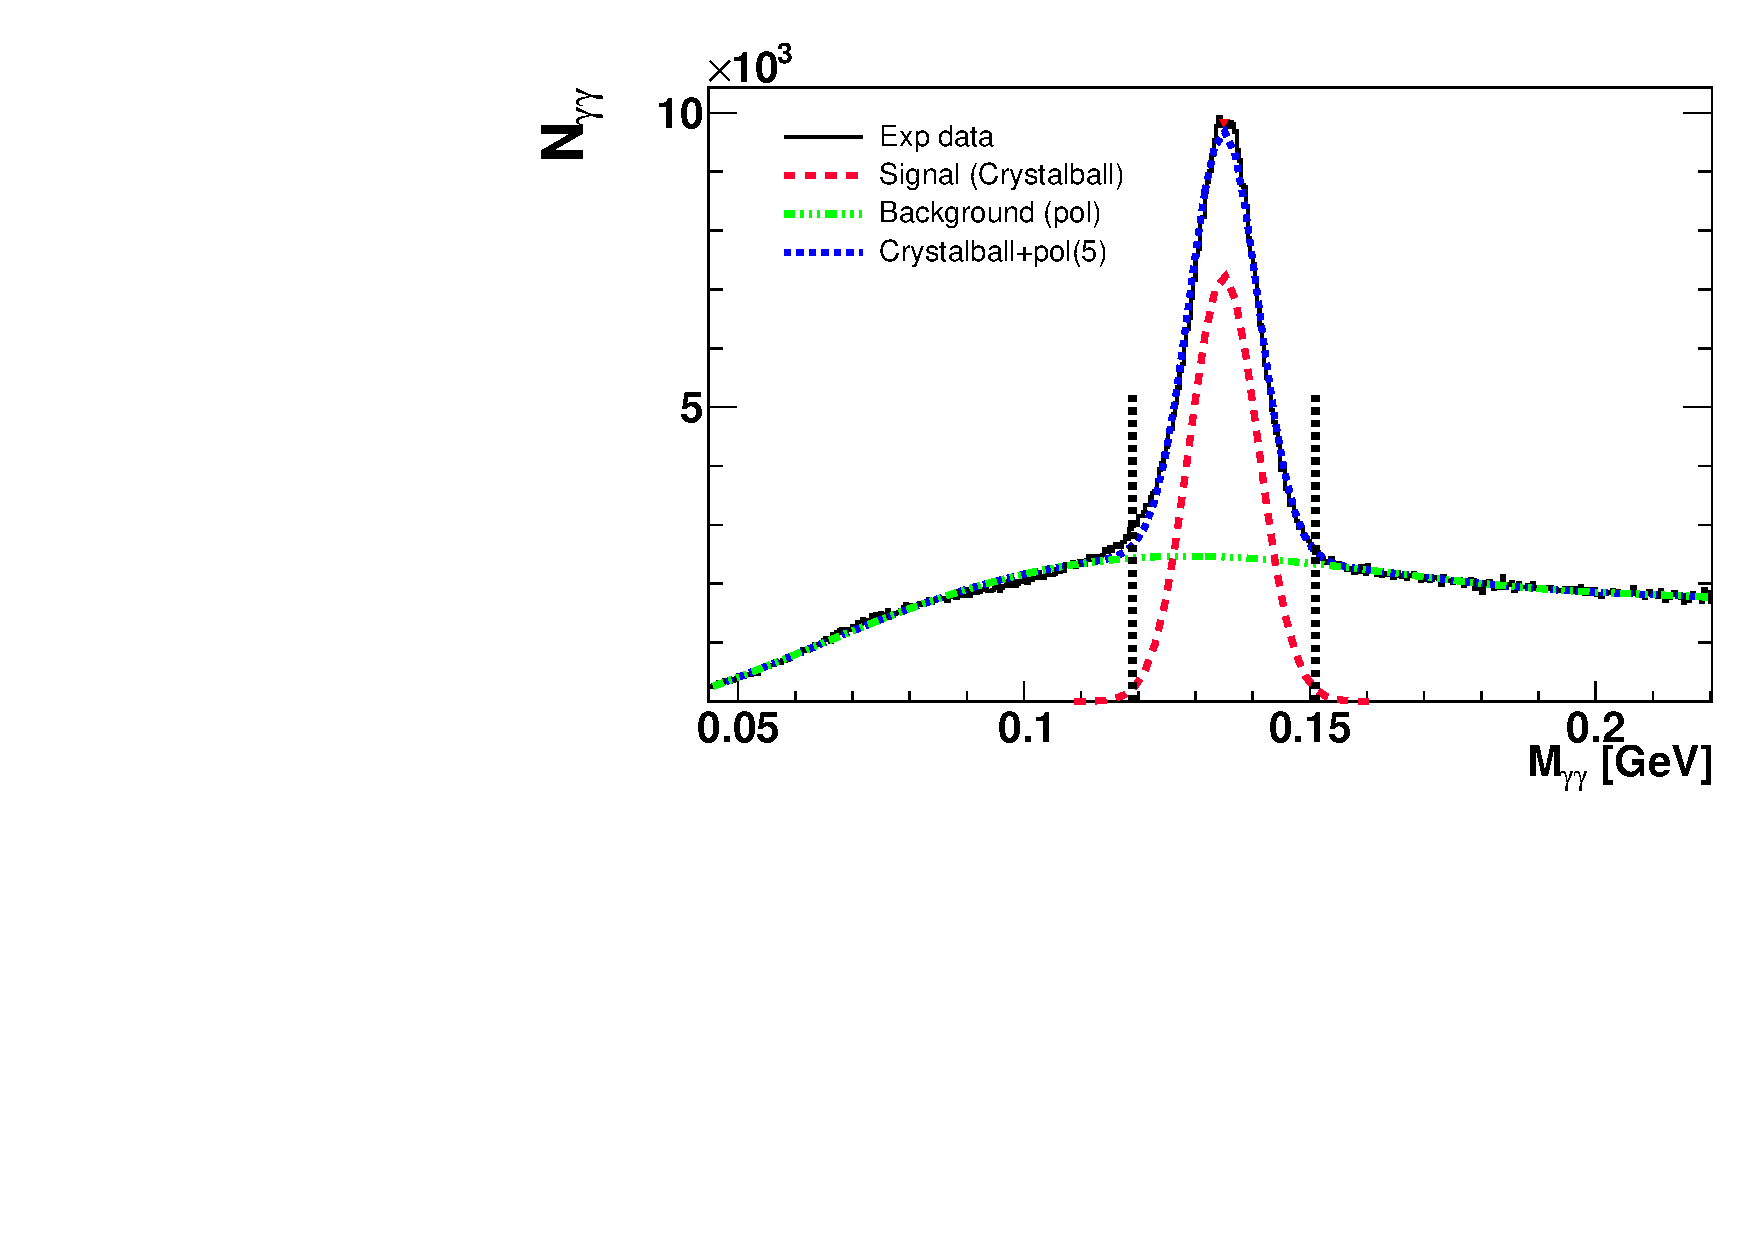
\includegraphics[width=.48\textwidth,natwidth=600,natheight=400]{figure_dataselection/pi0_crystalfit_Z_1.pdf}}
  \subfigure[$\pi^0$ invariant mass fit, $0.6<z<0.7$]{\label{fig:pi0crystalfit_4}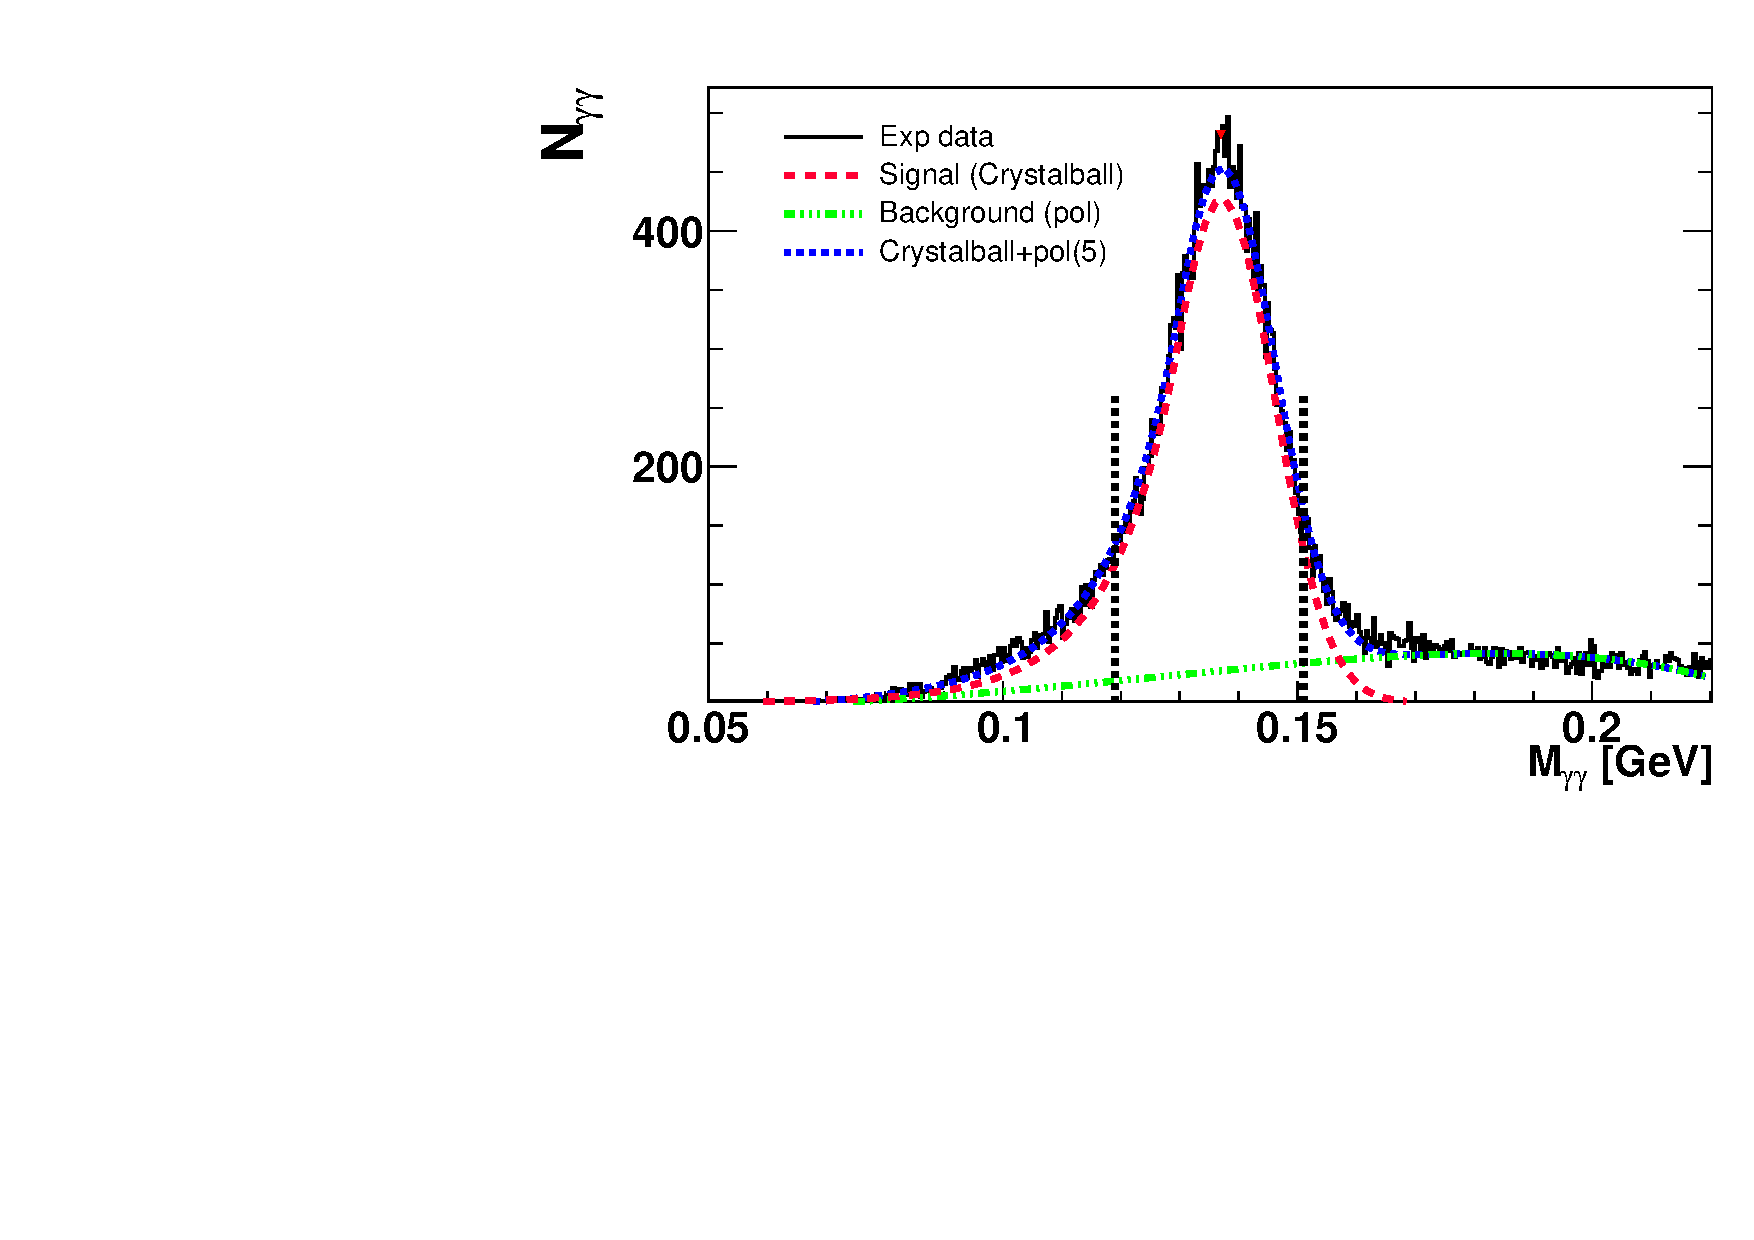
\includegraphics[width=.48\textwidth,natwidth=600,natheight=400]{figure_dataselection/pi0_crystalfit_Z_5.pdf}}
  \caption{Fit to the two-photon invariant mass distribution using a Crystal Ball function for the signal and a polynomial background function. In each plot, the green line represents the fitted background using a polynomial of 5th order, the red line the fitted signal and the blue line is the combined background and signal fit. It agrees well with the experimental data in black. The vertical dash lines are the boundaries that we will use to select the signal. See text for more details.}
  \label{fig:pi0_crystalfit}
\end{figure}

\subsubsection{Fit with Monte Carlo Background}
\label{sec:fit_with_MC_BG}

The fits presented in the previous section agree well with the experimental data. 
However, the question if we actually extract the correct background fraction is predicated on the condition that we get the signal and background shape correct.  One particular question is, how much the signal `bleeds' into the sideband region which has the most impact on the background fit. In this section we  develop an alternative, non-parametric method to extract the signal based on the shapes of signal and background as obtained from simulation. The advantage of this method is that it can differentiate between signal and background in regions where their shapes are similar. On the other hand, it relies of course on a correct description of the experimental data in the simulation.
%One of the main questions in the background evaluation is: Does 
%the event sample used for the BG obtained from the previous fits reflect 
%to a good degree the characteristics of the BG under the signal peak? 
%After all we want to separate the actual signal ("true" pi0) asymmetry 
%from the total asymmetry in this invariant-mass range by subtracting the 
%BG asymmetry. The latter has to be obtained from a different event sample 
%and if part of the sidebands is correlated with the signal asymmetry, 
%those sideband bins might not be a good proxy in the BG subtraction in particular since they can contain signal events where one of the decay $\gamma$ lost energy in pair creation (and one of the resulting leptons was misidentified as a $\gamma$). Hence 
%the studies presented in this section."
%Although the last section shows good fitting result, we still need to figure out if the components of the reconstruction are precisely described.
Some exemplary comparisons of the signal-background separated simulations with experimental data are shown in  Fig.~\ref{fig:pi0MC_Exp}. We observe that the agreement in the sidebands is quite good.  For low-$z$ and low-$P_t$ bins,  shown in Fig.~\ref{fig:pi0mcexp_1} and Fig.~\ref{fig:pi0mcexp_3} significant differences between Monte Carlo and experimental data can be seen in the signal region, seemingly caused by an overestimation of the signal yield in the MC. The agreement in the signal and background regions at high $P_t$ and high $z$ is quite good. 
\begin{figure}[H]
  \centering     
  \subfigure[$\pi^0$ invariant mass, $0<P_t<0.15$]{\label{fig:pi0mcexp_1}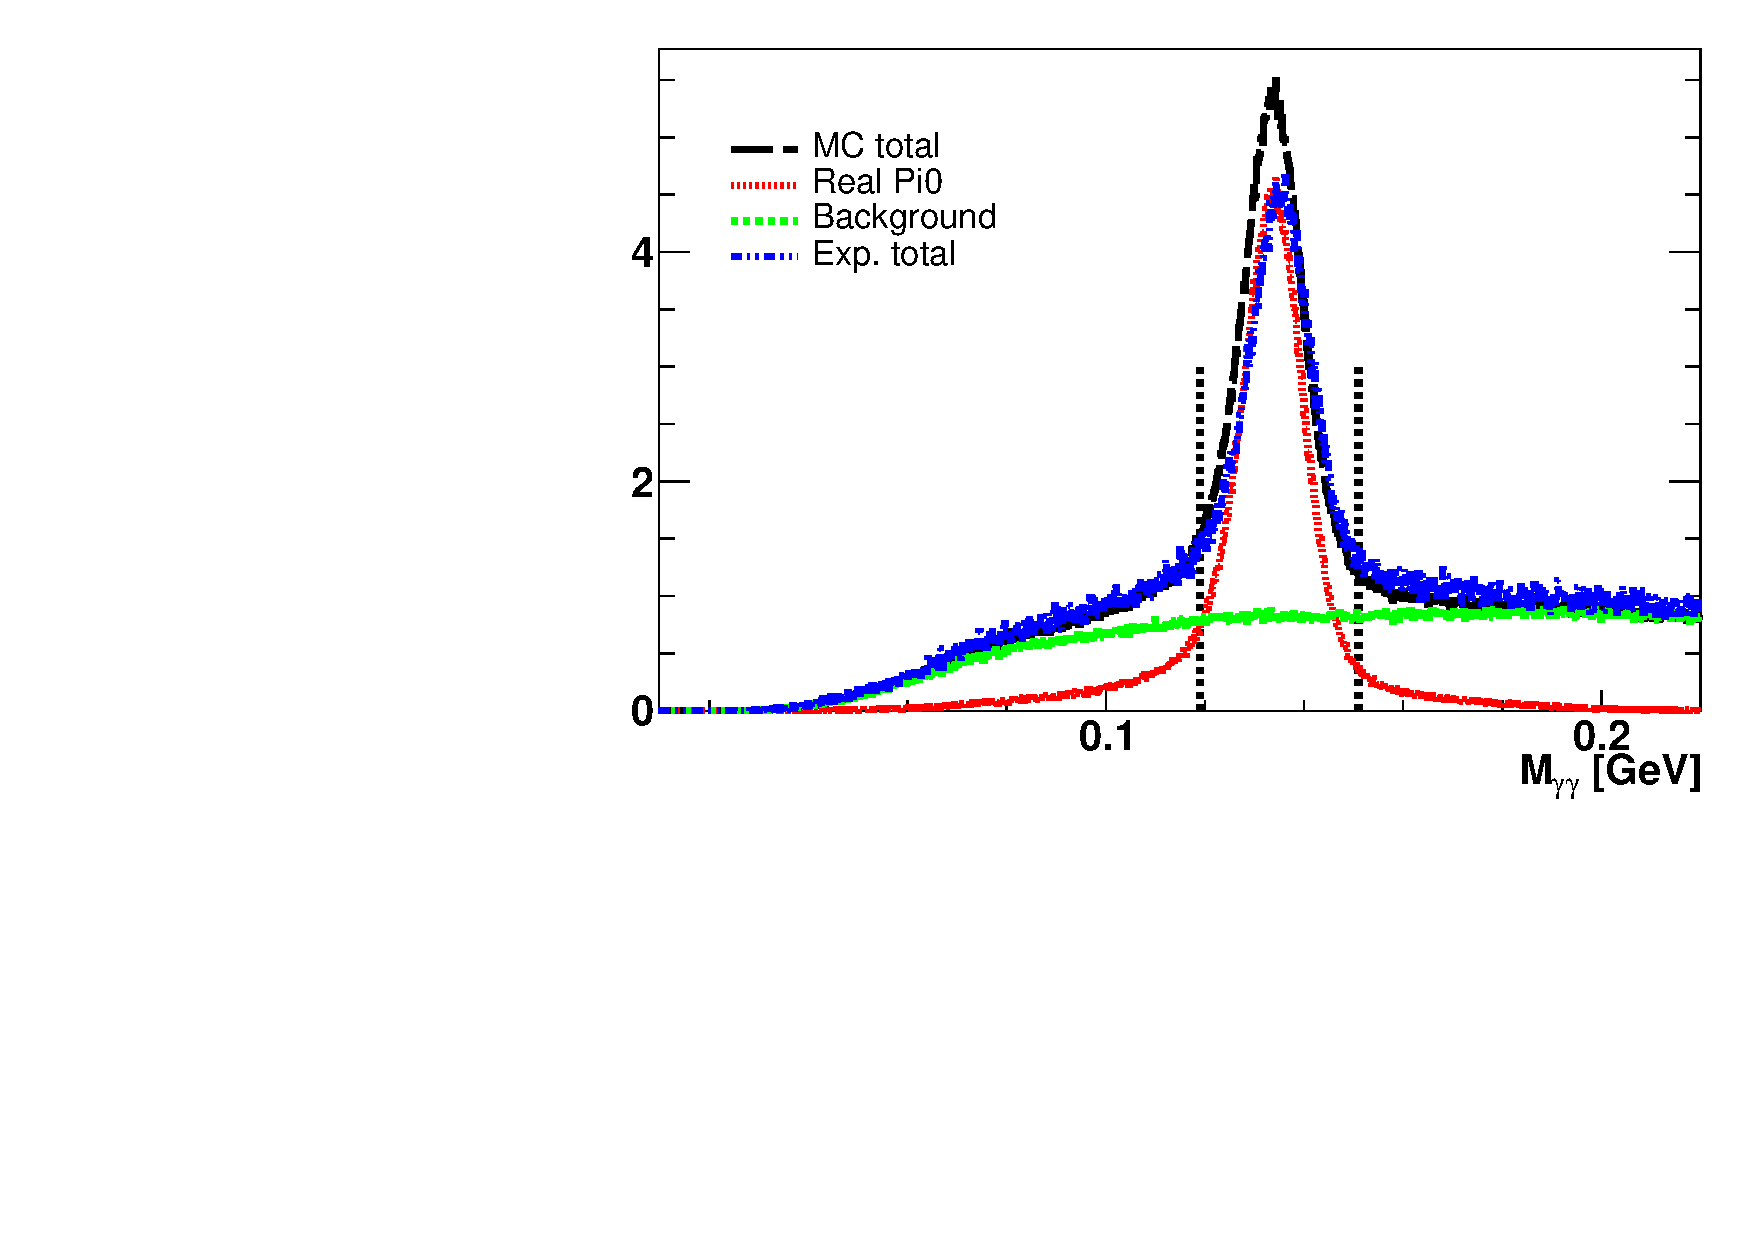
\includegraphics[width=.48\textwidth,natwidth=250,natheight=100]{figure_dataselection/pi0_Pt_0.pdf}}
  \subfigure[$\pi^0$ invariant mass, $0.3<P_t<0.5$]{\label{fig:pi0mcexp_2}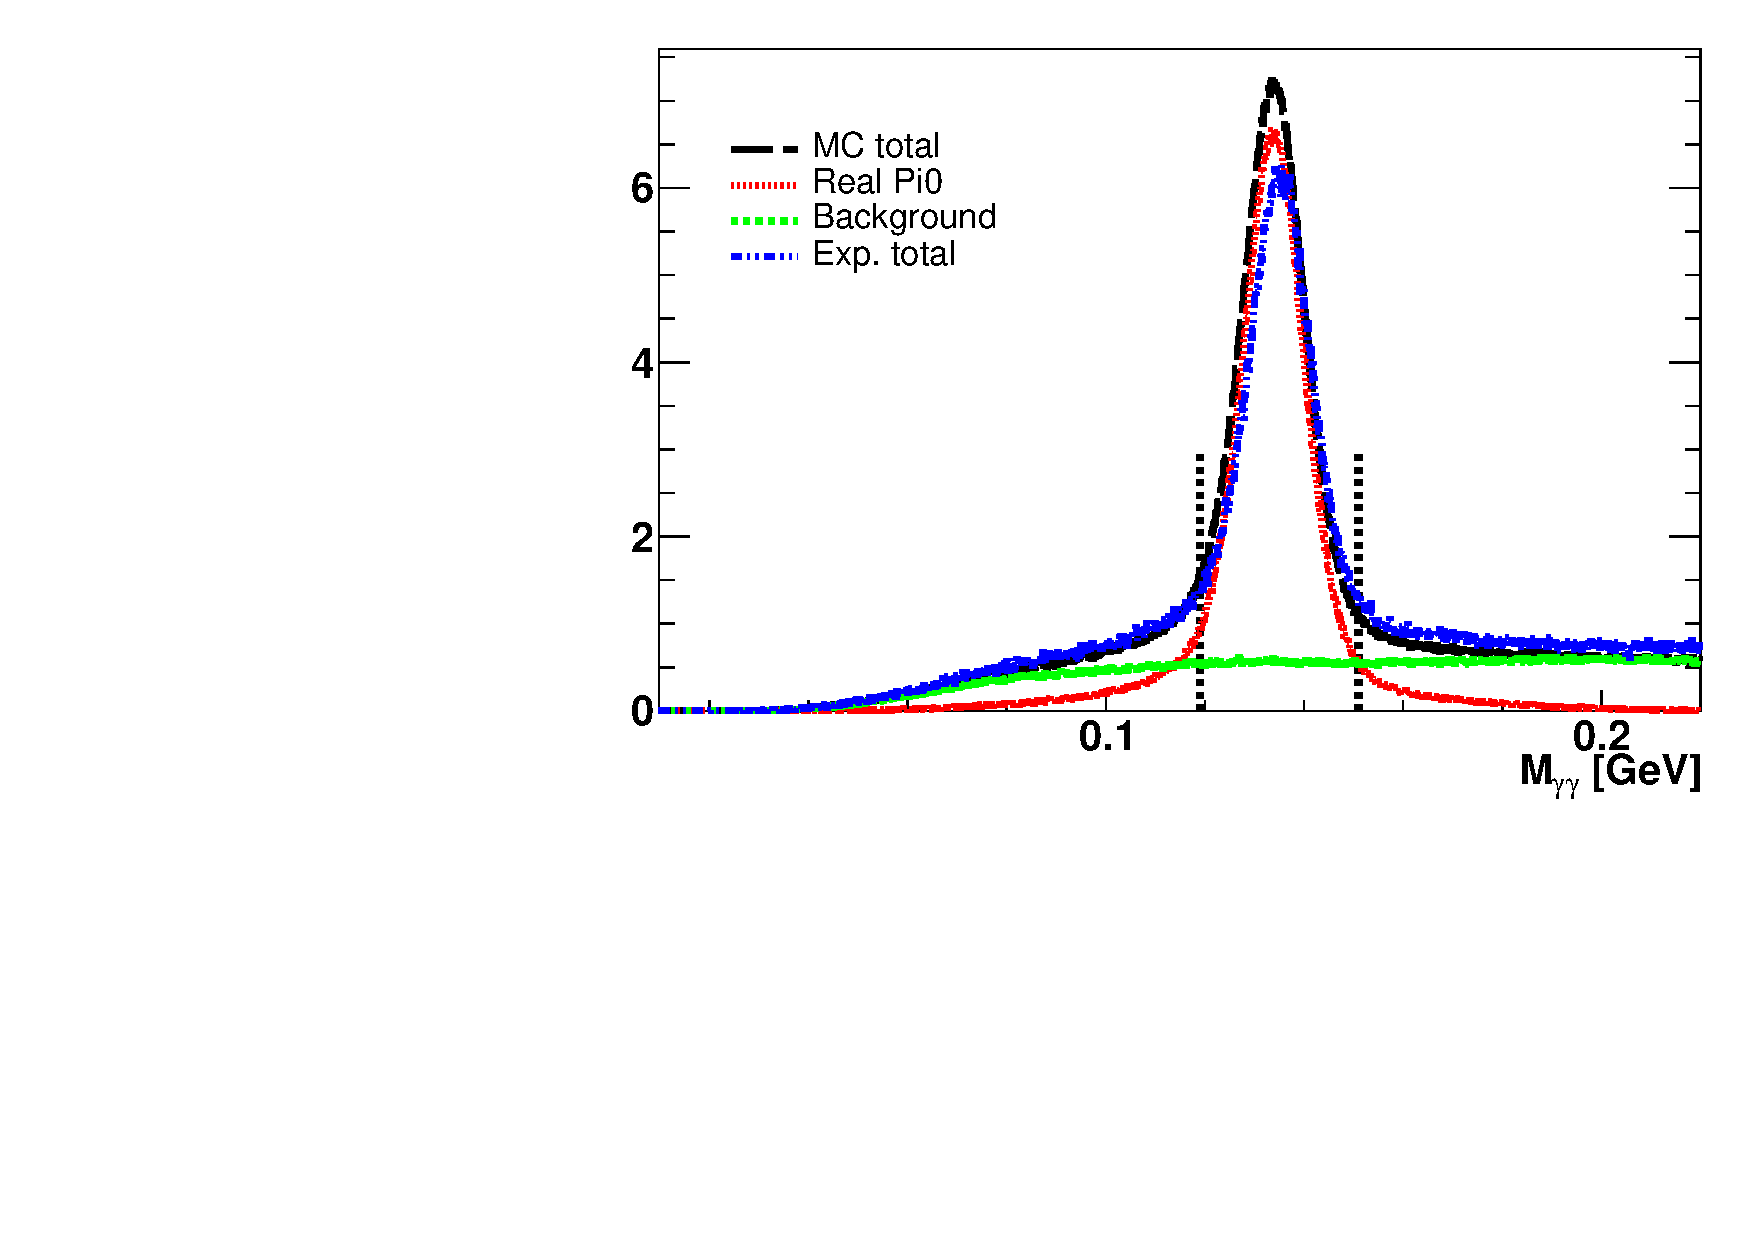
\includegraphics[width=.48\textwidth,natwidth=250,natheight=100]{figure_dataselection/pi0_Pt_2.pdf}}
   \subfigure[$\pi^0$ invariant mass, $0.2<z<0.3$]{\label{fig:pi0mcexp_3}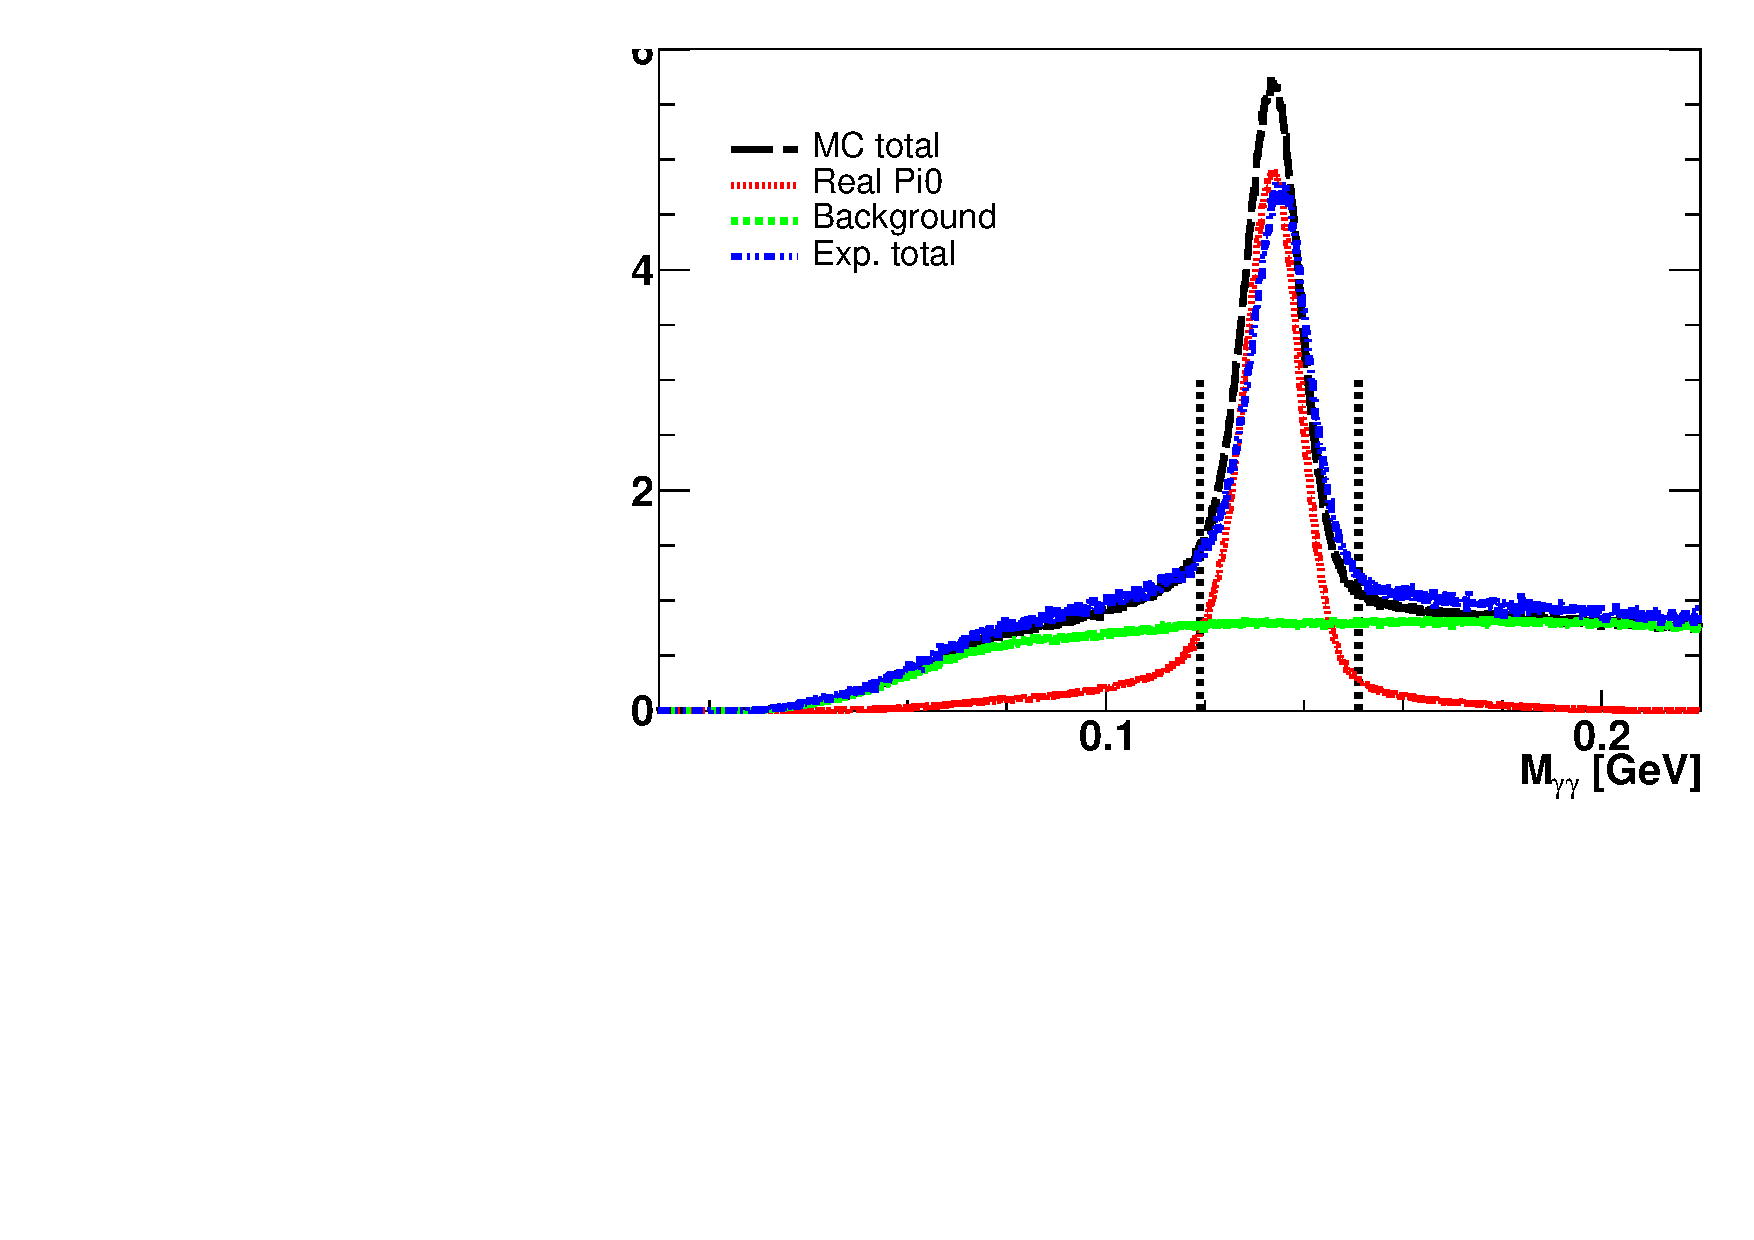
\includegraphics[width=.48\textwidth,natwidth=250,natheight=100]{figure_dataselection/pi0_Z_1.pdf}}
  \subfigure[$\pi^0$ invariant mass, $0.6<z<0.7$]{\label{fig:pi0mcexp_4}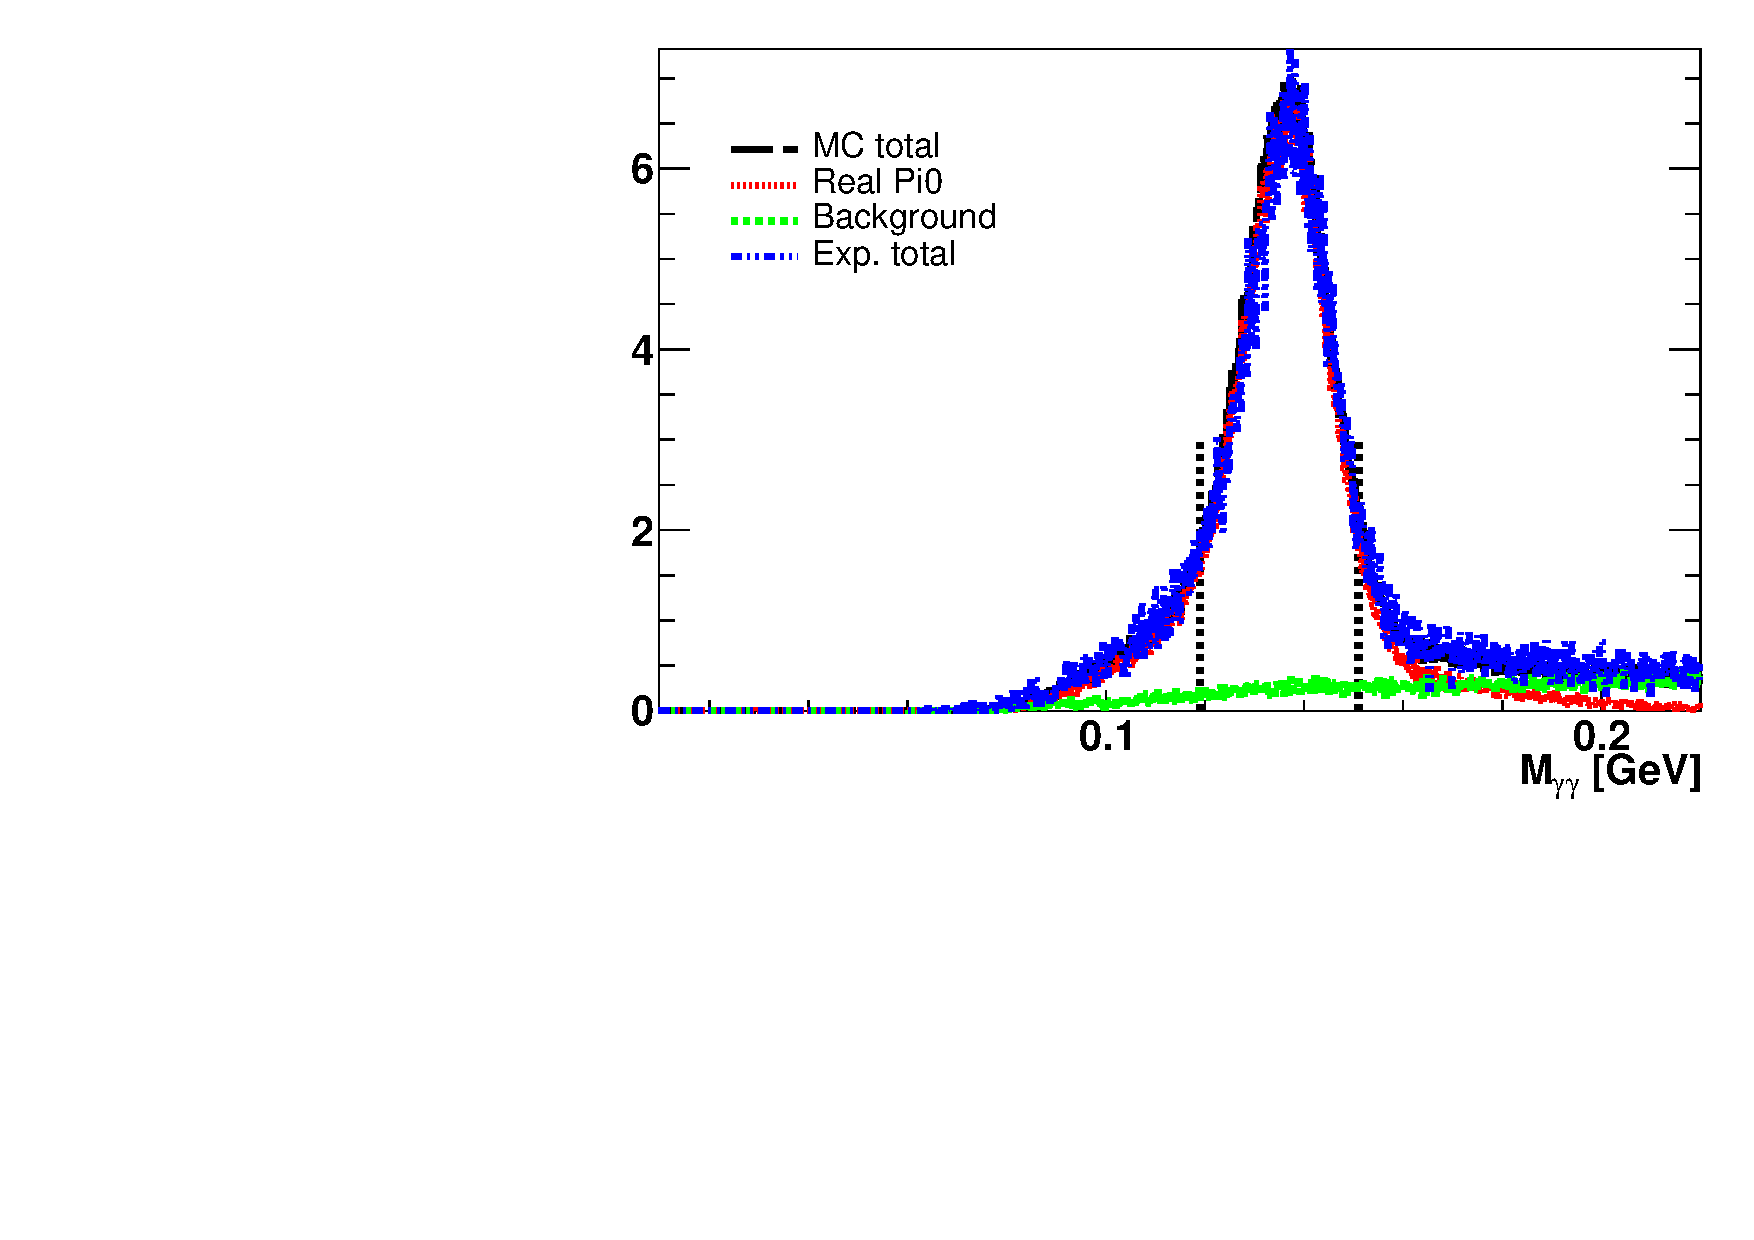
\includegraphics[width=.48\textwidth,natwidth=250,natheight=100]{figure_dataselection/pi0_Z_5.pdf}}
  \caption{Invariant mass of Monte Carlo vs. experimental data for some exemplary bins after applying all fiducial and energy constraints. The black line is the total Monte Carlo invariant mass. The blue line is the experimental invariant mass. The red line is the real $\pi^0$ signal identified by particle ID from Monte Carlo and the green line represents background in Monte Carlo. We define an identified photon pair as a ``real'' $\pi^0$ if both corresponding true particles have a common $\pi^0$ as a pararent. The vertical dash lines are the boundaries of the signal invariant mass window.}
  \label{fig:pi0MC_Exp}
\end{figure}


To address this problem of the overestimation of the signal region yield in the simulation, we divide the invariant mass range into upper and lower sidebands as well as a signal region. Our approach will be to fix the signal/bg ratio in the sideband regions, where the agreement is quite good and extrapolate the background under the signal peak.	 The range of the lower sideband is $0.014$~GeV$\textup{--}0.112$~GeV. In this region, shapes of both simulation and data agree. Hence, for this region, experimental background is estimated using Eq.~\eqref{eqn:pi0fitfunction1}, in which $N_i^{bg}$ is the experimental background of invariant mass bin $i$ and $N_i^{tot}$ is the experimental total yield of bin $i$. $N_i^{MCtot}$ and $N_i^{MCbg}$ represent the MC and MC background content of bin $i$, respectively.  
\begin{equation}
N_i^{bg}=\frac{N_i^{tot}}{N_i^{MCtot}}*N_i^{MCbg}
\label{eqn:pi0fitfunction1}
\end{equation}
Or in other words, we assume the same background fraction in the MC simulation and the experimental data and thus apply the one obtained from the MC simulation to the experimental-data yields in order to obtain the experimental BG yield, and do that for each invariant-mass bin separately.


As shown in Fig.~\ref{fig:pi0MC_Exp} experimental data and MC have the similar shape in the upper sideband region from $0.146$~GeV to $0.22$~GeV and we therefore also use Eq.~\eqref{eqn:pi0fitfunction1} to fit this region. The idea of background fitting is a simple conversion between MC to experimental data.

The signal region is $0.112$~GeV$\textup{--}0.146$~GeV. As the shapes of MC and experimental data are quite different, especially the peak position changes slightly, a simple conversion doesn't work here. Fortunately the background in this section is smooth in MC and a polynomial function of order 2 connecting upper and lower sidebands can be used to estimate background.
The fit connecting the upper and lower sidebands uses 20 points on each side covering $\pm 0.02$ on each side.

Finally, the signal is obtained by subtracting the background shape from the experimental data. Fig.~\ref{fig:pi0_fit} shows the fit result of $\pi^0$.  
\begin{figure}[H]
  \centering     
  \subfigure[$\pi^0$ invariant mass fit, $0<P_t<0.15$]{\label{fig:pi0fit_1}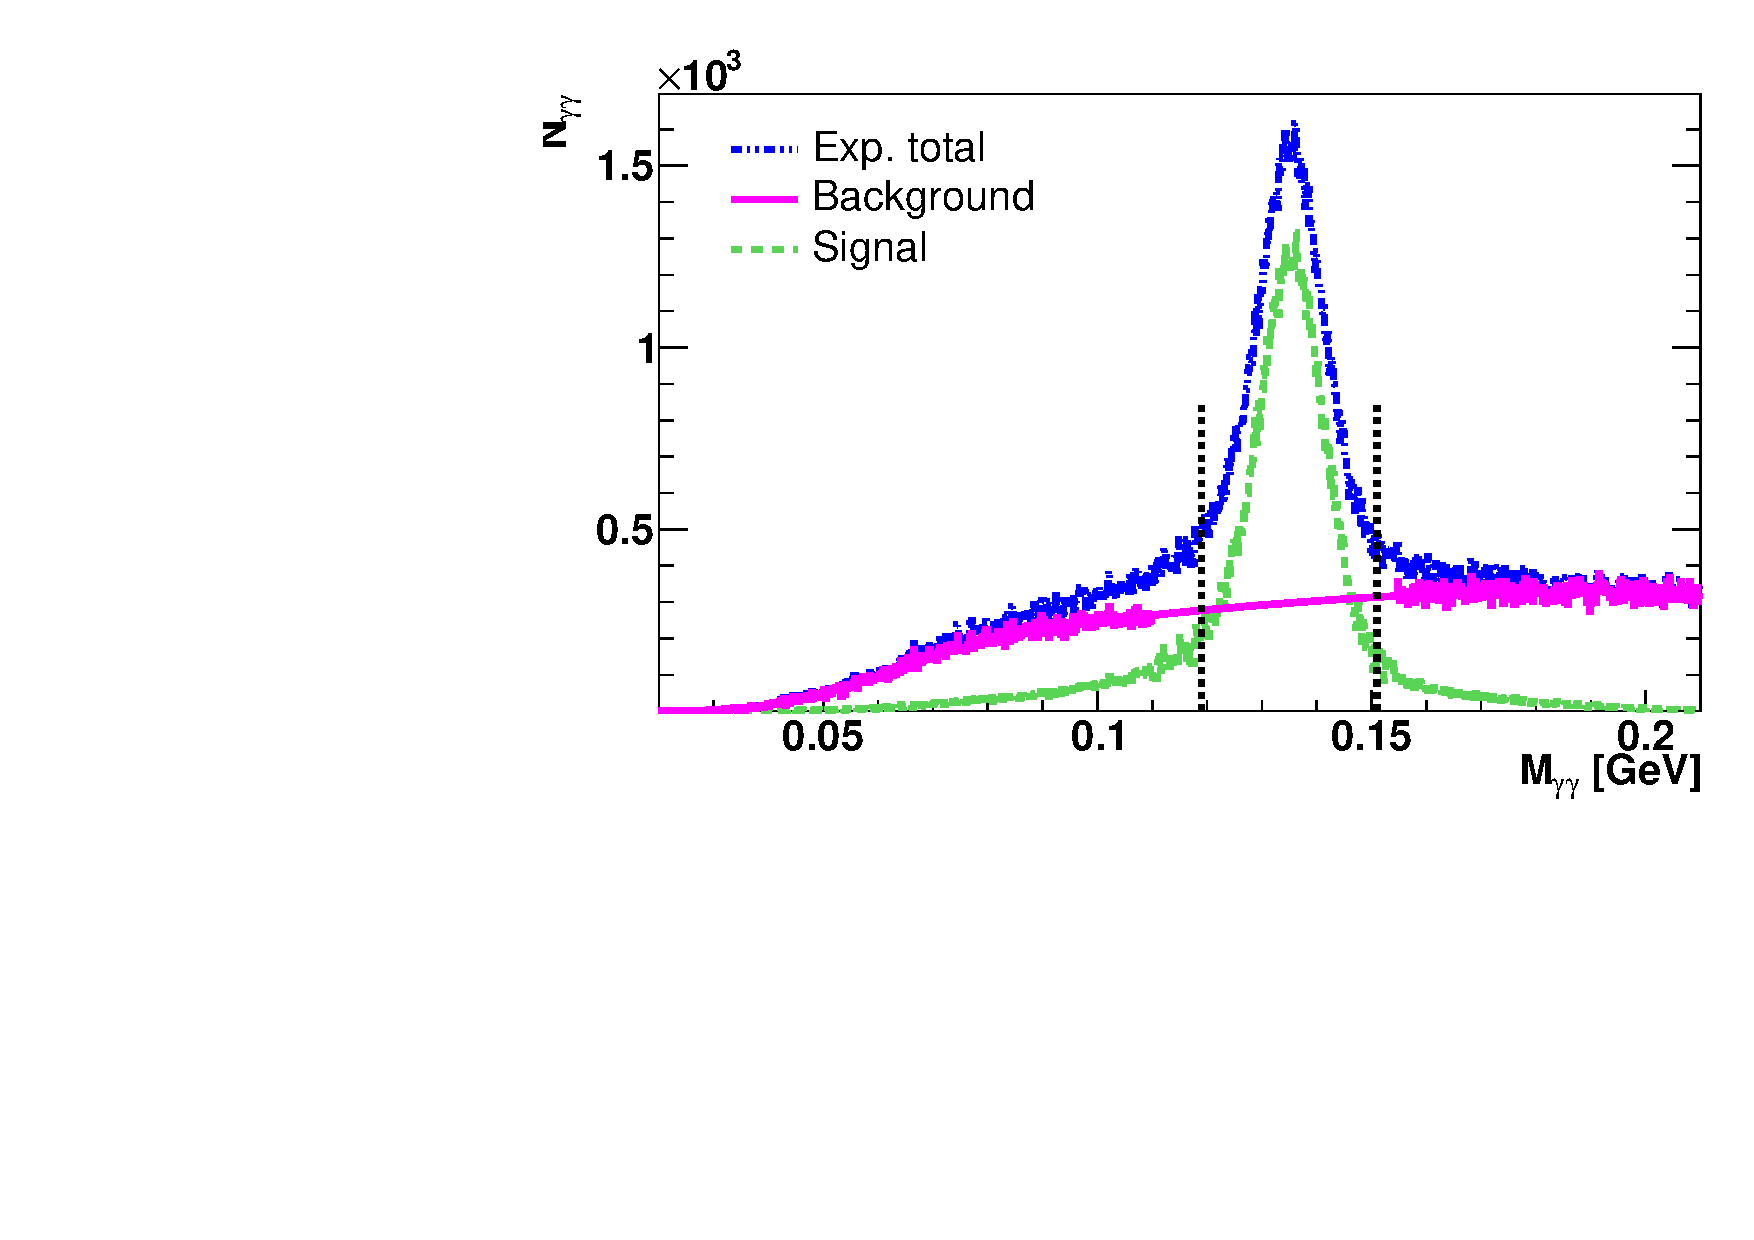
\includegraphics[width=.48\textwidth,natwidth=600,natheight=400]{figure_dataselection/pi0_fit_Pt_0.pdf}}
  \subfigure[$\pi^0$ invariant mass fit, $0.3<P_t<0.5$]{\label{fig:pi0fit_2}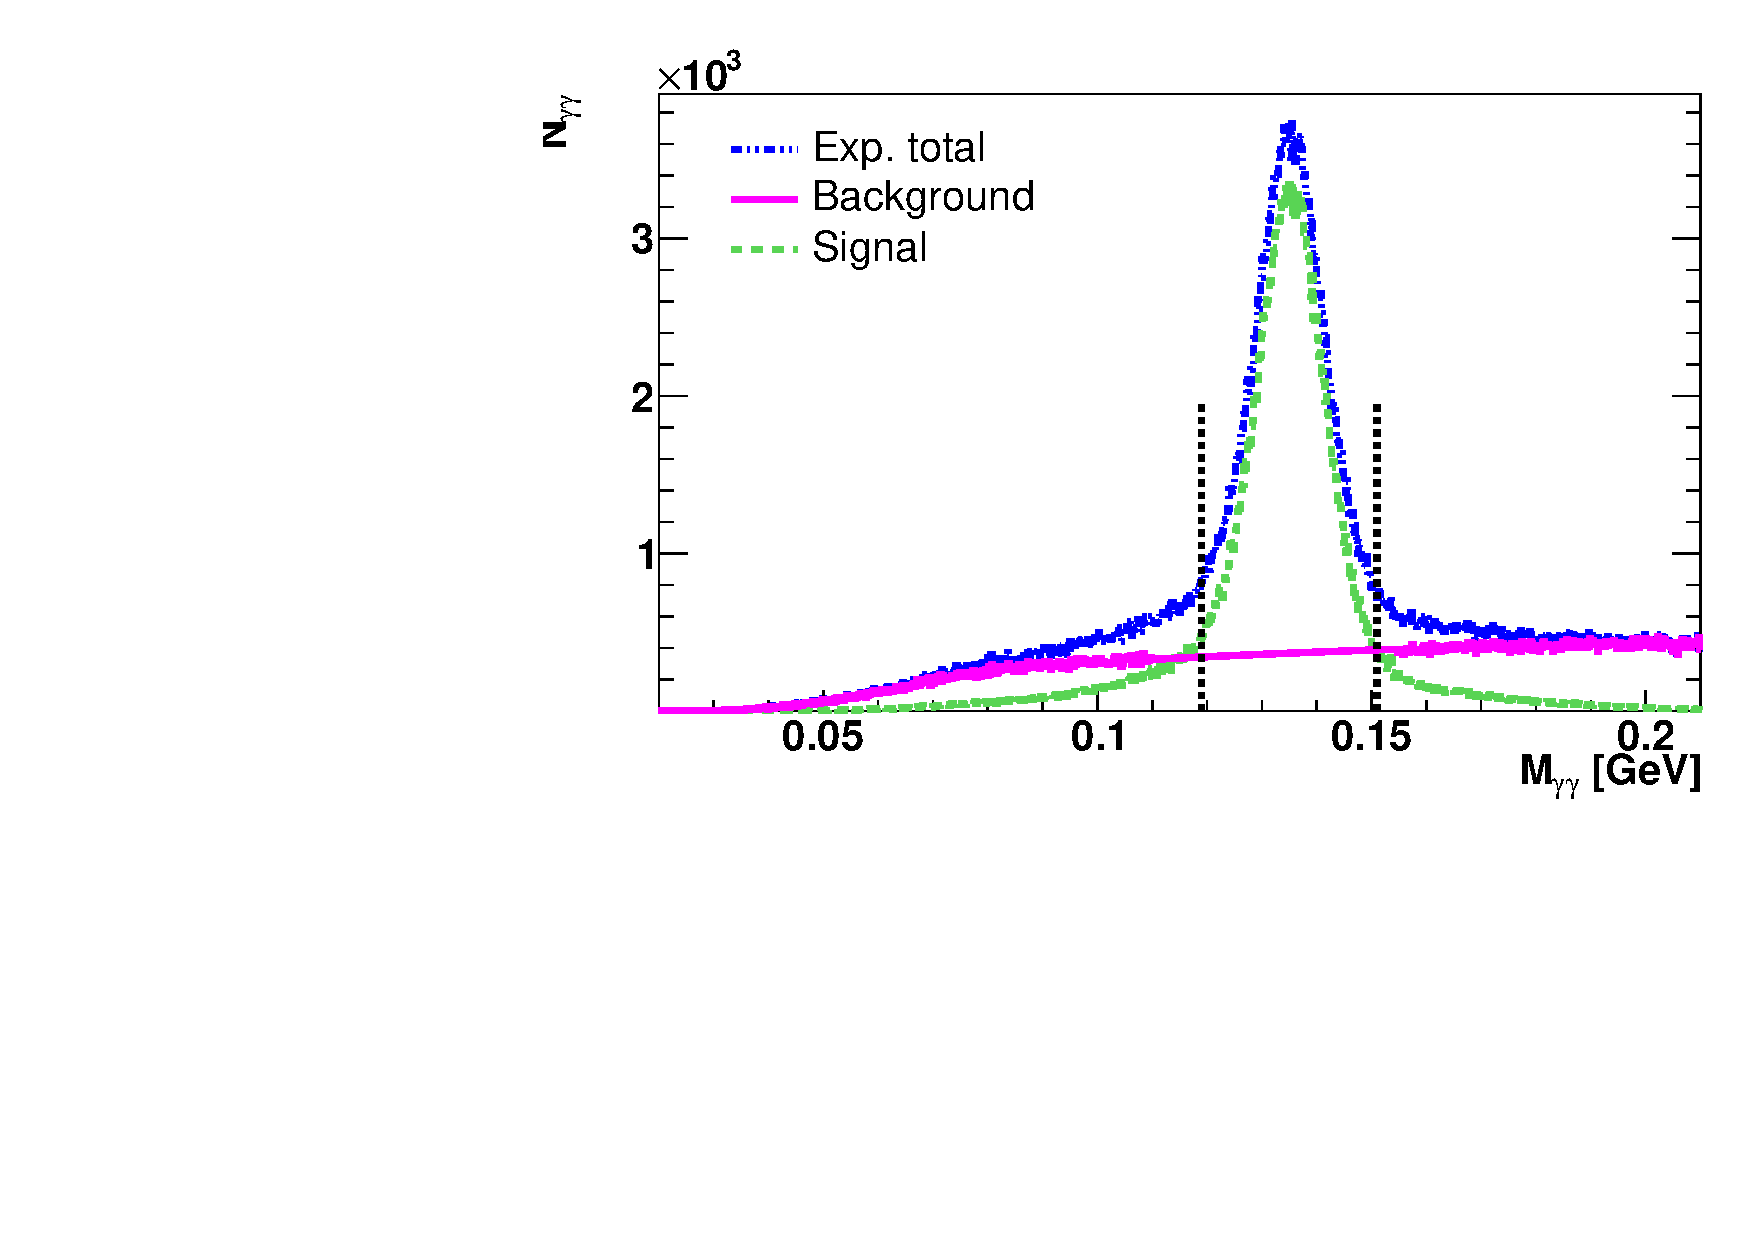
\includegraphics[width=.48\textwidth,natwidth=600,natheight=400]{figure_dataselection/pi0_fit_Pt_2.pdf}}
  \subfigure[$\pi^0$ invariant mass fit, $0.2<z<0.3$]{\label{fig:pi0fit_3}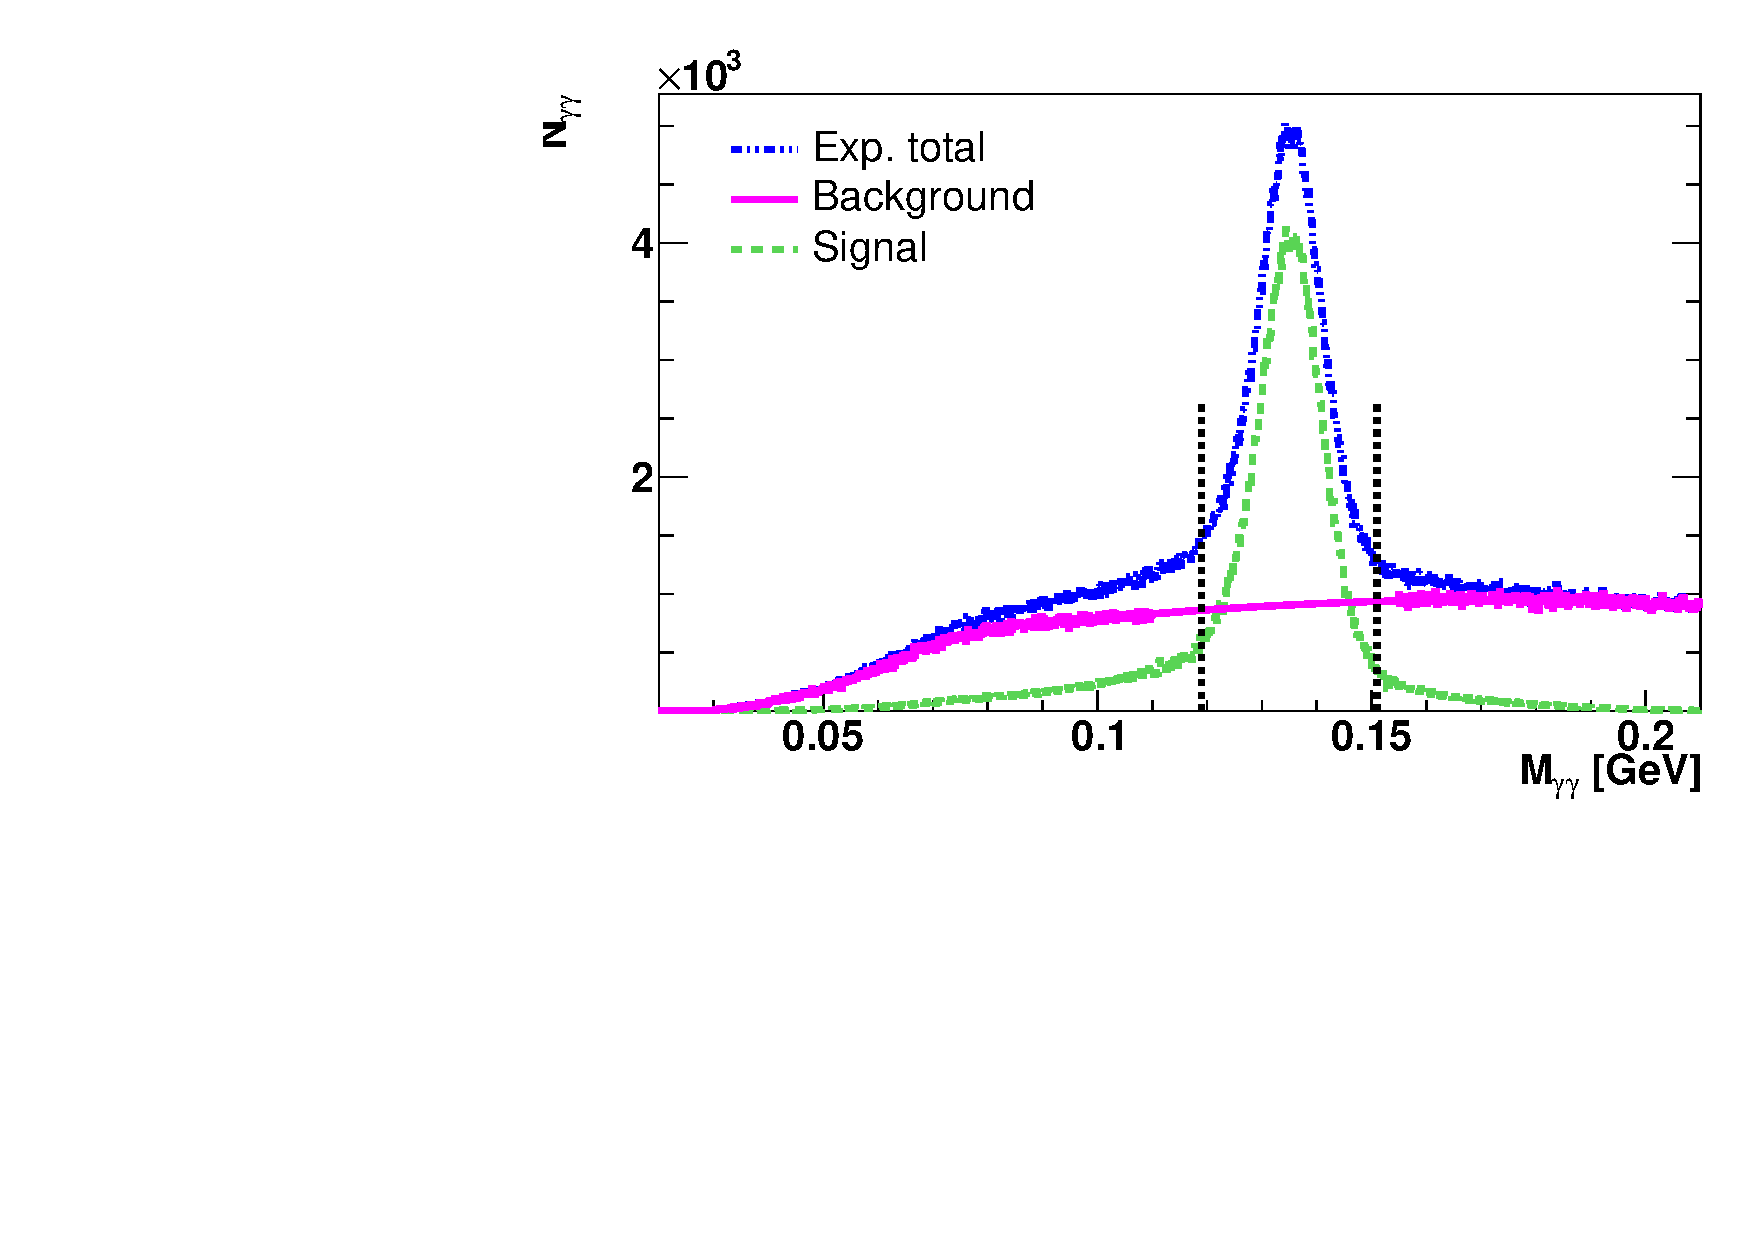
\includegraphics[width=.48\textwidth,natwidth=600,natheight=400]{figure_dataselection/pi0_fit_Z_1.pdf}}
  \subfigure[$\pi^0$ invariant mass fit, $0.6<z<0.7$ ]{\label{fig:pi0fit_4}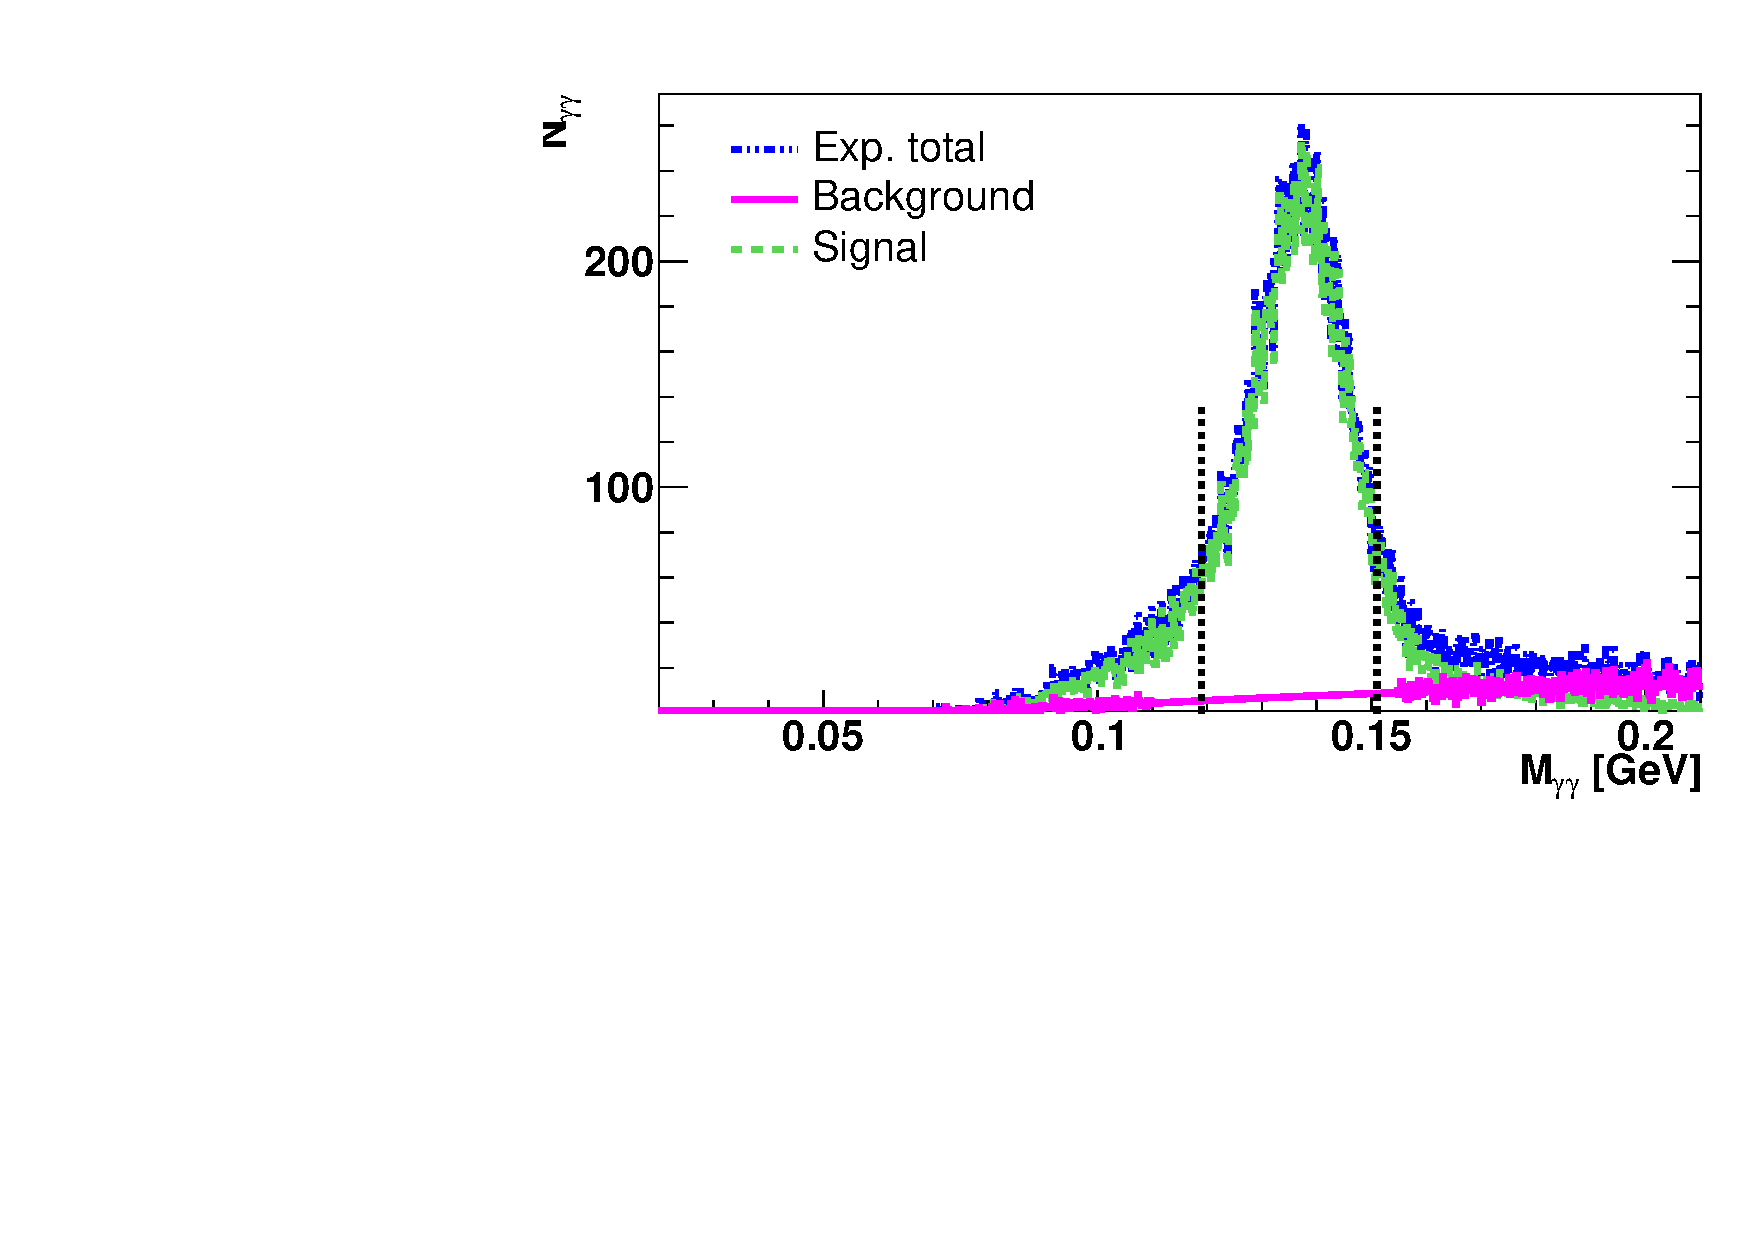
\includegraphics[width=.48\textwidth,natwidth=600,natheight=400]{figure_dataselection/pi0_fit_Z_5.pdf}}
  \caption{Nonparametric fit of the experimental data using the MC background shape. The blue line is the total experimental data. The purple line is the background which has the same shape with background in MC. The green dash line is the signal obtained by subtracting the background from the total yield in the signal region. The vertical dash line is again the signal window. }
  \label{fig:pi0_fit}
\end{figure}

In order to evaluate the parametric Crystal-Ball and the non-parametric methods for the $\pi^0$ extraction presented in this section, we compare the obtained signals in Fig.~\ref{fig:pi0mcexpsig} with the signal from the simulation. 
Note that here the signal in Monte Carlo also comes from the direct reconstruction of the $\gamma$'s instead of using the $\pi^0$ particle table provided by the Belle MC. Section~\ref{sec:sysStudies} discusses the signal and background identification in some more detail. In short, we define all reconstructed $\gamma$ pairs as background, where the corresponding true particles cannot be traced back to a common $\pi^0$ parent (or $\eta$ when we want to reconstruct those, but in this channel the backgrounds are small). 

The results in Fig.~\ref{fig:pi0mcexpsig} show a discrepancy in the extracted signals between the methods in the lower $z$ and $P_t$ bins. In particular, the MC signal shape has longer tails towards lower invariant masses. This leads to a lower estimation of the background in the signal region, which in turn leads to a larger extracted signal compared to the Crystal-Ball method. The MC signal is larger than both methods, reflecting the data-simulation difference. The data/MC difference only impacts the non-parametric method. We think that assigning the difference between the two methods as a systematic effect captures a signal shape that is different from the Crystal-Ball method (assumed for the parametric method) and potential effects from the data/mc disagreement on the non-parametric method.. It should be noted, that we show later in~\ref{sec:backgroundcorrection} that the sidebands also carry an asymmetry that is close to the signal region. This helps suppress any systematic effect on the estimation of the signal fraction.
%Given that the sidebands also carry a sizeable asymmetry that is actually of similar magnitude than the signal region (see sec.~\ref{sec:backgroundcorrection} ), we think that the any effect of the data/mc difference 

%In Fig.~\ref{fig:pi0mcexpsig}, the signal region in the experimental data exceeds the signal distribution in the MC simulation for the lower $z$ bins. This can already be seen in the total invariant-mass distributions.
% In addition, the two extraction methods give different signals.The high-z bin presented shows better agreement of the $\pi^0$ peaks. 
%Section~\ref{sec:backgroundcorrection} shows that because the background has asymmetries at the same level as signal the uncertainty of purity, defined as signal over total data, does not contribute much to the systematic uncertainty. 

%For the final results we use the Crystal Ball fit 

%Since there is evidence that the simulated background shape agrees with experiment, e.g. from the sidebands in fig.~\ref{fig:pi0_fit} and our studies presented in sec.~\ref{sec:backgroundcorrection} show that the sidebands have in fact a similar 
%Since the background shapes on the other hand show good agreement between data and MC and we know from Section~ that uncertainties in the purity in the signal region can be neglegted due to the similar size of the background and signal asymmetries, we do not consider data-MC difference in the MC region for small $z$ in our systematic uncertainties. We think that any differences between data and simulation are mainly important for the background estimation and are captured in assigning the difference between the two fit methods as a systematic uncertainty.

 The Crystal Ball method leads to a proper fitting result of $\eta$, see section~\ref{sec:etafitsection}, so in order to make the analysis consistent we adopt the Crystal Ball method for $\pi^0$ as well. The difference between the the two signal extraction methods will be included as part of systematic uncertainties.
\begin{figure}[H]
  \centering     
  \subfigure[ $0$~GeV$<P_t<0.15$~GeV]{\label{fig:pi0mcexpsig_1}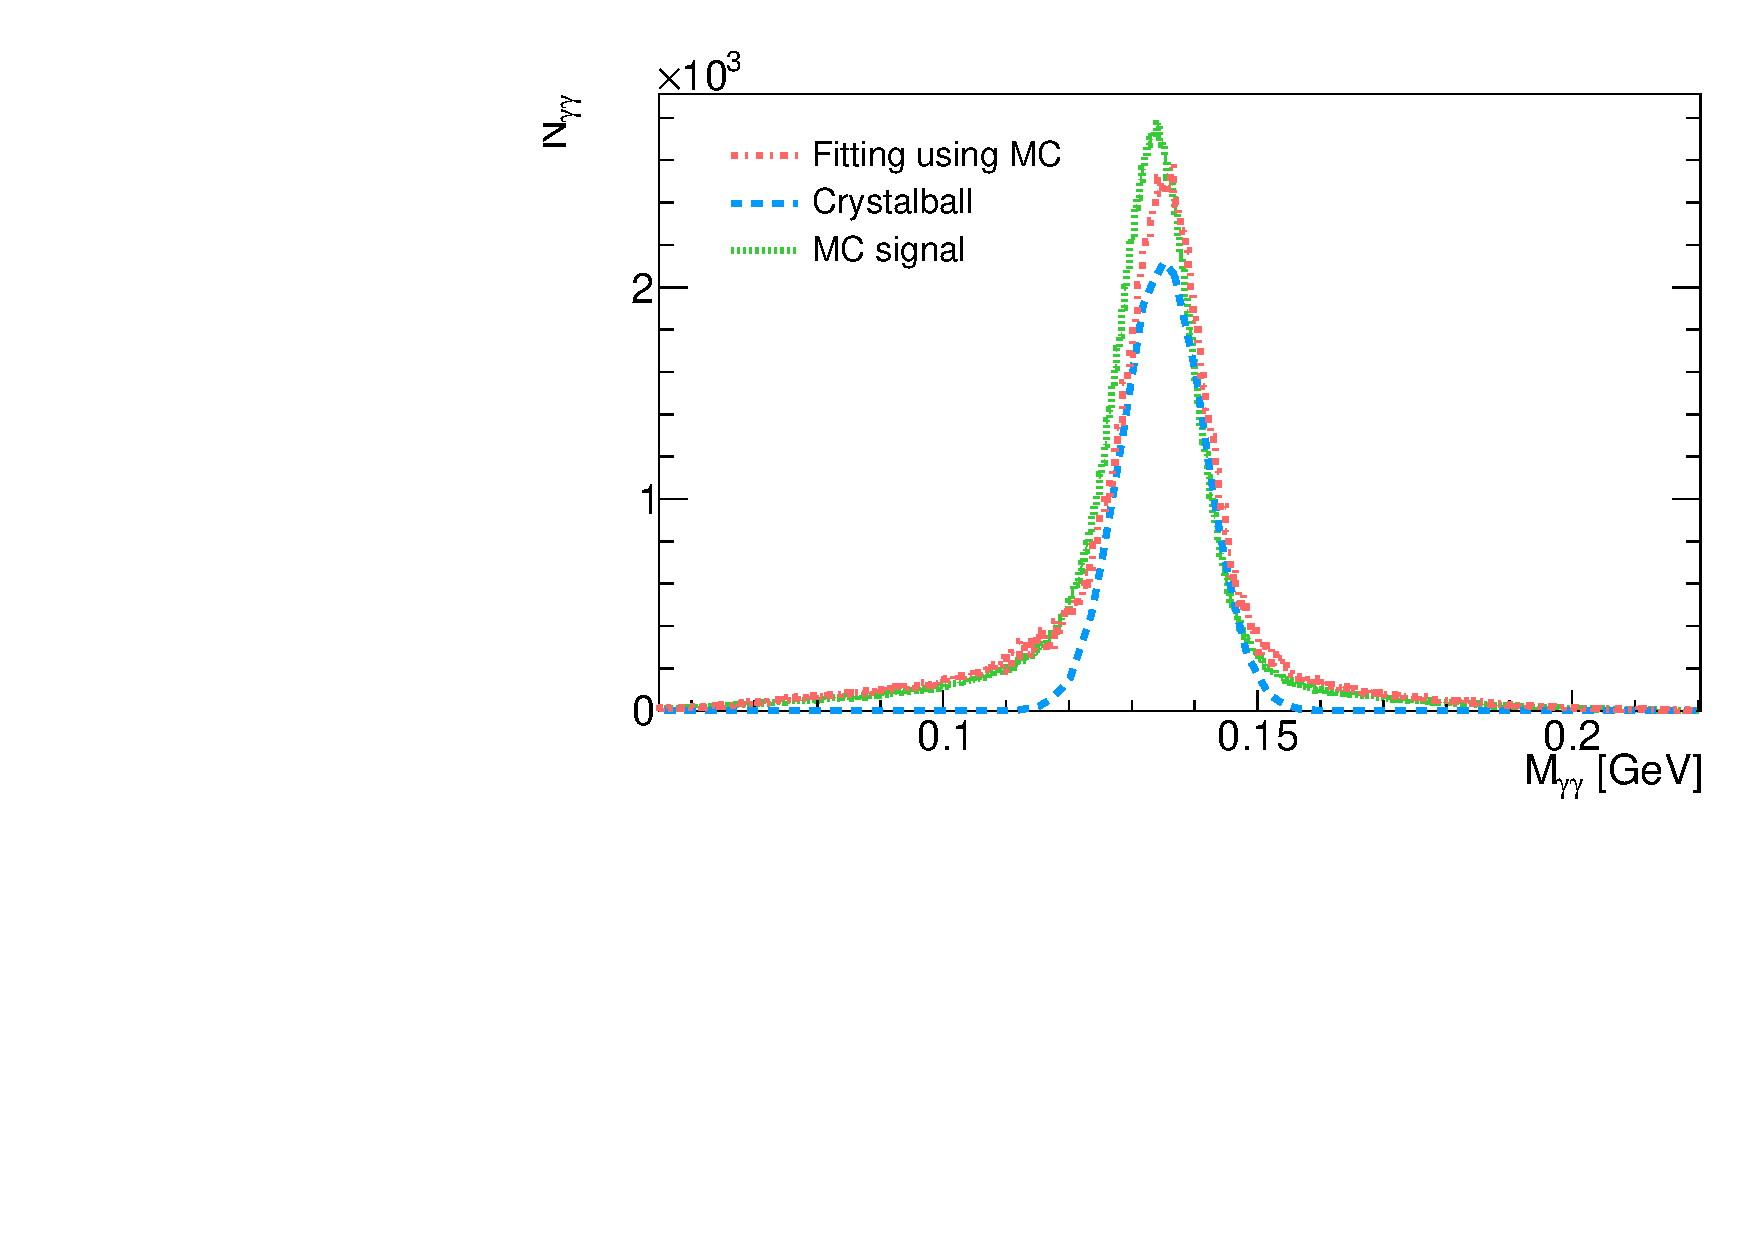
\includegraphics[width=.48\textwidth,natwidth=600,natheight=400]{figure_dataselection/fitting_signal_compare_Pt0.pdf}}
  \subfigure[$0.3$~GeV$<P_t<0.5$~GeV]{\label{fig:pi0mcexpsig_2}\includegraphics[width=.48\textwidth,natwidth=600,natheight=400]{figure_dataselection/fitting_signal_compare_Pt2.pdf}}
  \subfigure[$0.2<z<0.3$]{\label{fig:pi0mcexpsig_3}\includegraphics[width=.48\textwidth,natwidth=600,natheight=400]{figure_dataselection/fitting_signal_compare_Z1.pdf}}
  \subfigure[$0.6<z<0.7$]{\label{fig:pi0mcexpsig_4}\includegraphics[width=.48\textwidth,natwidth=600,natheight=400]{figure_dataselection/fitting_signal_compare_Z5.pdf}}
  \caption{Signals from Monte Carlo and experiment. The green line is the Monte Carlo $\pi^0$ signal and the  red/blue line are the experimental signal.}
  \label{fig:pi0mcexpsig}
\end{figure}

\subsubsection{\texorpdfstring{Invariant Mass Fit of $\eta$}{eta fit} }
\label{sec:etafitsection}
The background shape under the $\eta$ peak is consistent between the upper and lower sidebands, in fact it can almost be described as a linear function. In the spirit of the previous section, we tried two different approaches. 
In the first, we fit the background separately in the upper and lower sidebands 
%(046.~GeV-0.45~GeV and 0.6~GeV-0.69~GeV), 
extrapolated through the signal region and obtained the signal by subtracting the background from the total data. The second method is the same as we used in the $\pi^0$ case, described above; We use a 5th order polynomial together with a Crystal Ball function (see Eqn.~\ref{eqn:crystalball} and reference~\cite{CrystalBallFunc}) to fit background and signal simultaneously. 


\begin{figure}[h]
\centering     %%% not \center
\subfigure[$0.5<z<0.6$]{\label{fig:etaz4fitbkg}\includegraphics[width=.48\textwidth,natwidth=600,natheight=400]{figure_dataselection/eta_fitbkg_Z_4.pdf}}
\subfigure[$0.5<z<0.6$]{\label{fig:etaz4fitall}\includegraphics[width=.48\textwidth,natwidth=600,natheight=400]{figure_dataselection/eta_fitall_Z_4.pdf}}
\caption{$\eta$ invariant mass for $z$ bin 4 in experimental data. In Fig.~\ref{fig:etaz4fitbkg}, the black line is the total experimental data, the green dotted line is a 4th-order polynomial and the blue line is the signal that is obtained by subtracting the red line from all data. In Fig.~\ref{fig:etaz4fitall}, the black line is the total data, the red line is the Crystal Ball function, the green line is a 5th-order polynomial and the turquoise line is the sum of Crystal Ball function and 5th-order polynomial function.}
\label{fig:eta_fit}
\end{figure}

 Figure~\ref{fig:eta_fit} shows the fit results and Fig.~\ref{fig:etasignal} displays the signals arising from those two methods. It can be seen that these methods give similar fitting results. However, for consistency reasons we use the Crystal Ball function plus the 5th order polynomial, since the same function can also be used to fit the $\pi^0$.

\begin{figure}[H]
\centering
\includegraphics[width=0.8\textwidth,natwidth=610,natheight=642]{figure_dataselection/eta_Signal_Z_4.pdf}
\caption{The red line is the fit result of the Crystal Ball function for the $\eta$ signal. The blue line is the signal from simply subtracting the background fitted from the total distribution. The plotted data has $0.5<z<0.6$.}
\label{fig:etasignal}
\end{figure}

\subsubsection{\texorpdfstring{Mass Window to Select $\pi^0$ and $\eta$}{Mass Window to Select pi0 and eta}}
\label{sec:masswindow}
In this section we describe how we choose the optimal mass window in the two-photon invariant mass spectrum 
 to select $\pi^0$ and $\eta$. The obvious issue is that a smaller mass window will lead to a higher $signal/background$ ratio but also to a reduction in signal yield. Fig.~\ref{fig:pi0ST} shows the relative signal contribution for various mass ranges. Fig.~\ref{fig:pi0SST} shows the $S/\sqrt{N}$ ratio, which is the figure of merit (FOM) we use, of different mass window widths for $\pi^0$, where $N$ is the total yield and $S$ is the signal. The mass window is centered around $0.135$~GeV, which is the world average mass for the  $\pi^0$. We define the mass window width to be half  the mass range. For example with width $0.005$, the mass window is $0.130$GeV$\textup{--}0.140$GeV. Both purity and yield factors are taken into account when selecting the mass window. Fig.~\ref{fig:etaS} shows the FOM of $\eta$.
\begin{figure}[h]
\centering     %%% not \center
\subfigure[$S/N$ ratio of $\pi^0$]{\label{fig:pi0ST}\includegraphics[width=60mm]{figure_dataselection/pi0_signal_ratio_crystalballfit.eps}}
\subfigure[$S/\sqrt{N}$ ratio of $\pi^0$]{\label{fig:pi0SST}\includegraphics[width=60mm]{figure_dataselection/pi0_STT_ratio_crystalballfit.eps}}
\caption{Two ratios related to the $\pi^0$ mass window selection. Different colors/line styles are ratios for different $z$ and $P_t$ bins. The horizontal axis is mass-window width~(see text for details).}
\label{fig:pi0S}
\end{figure}

\begin{figure}[h]
\centering     %%% not \center
\subfigure[$S/N$ ratio of $\eta$]{\label{fig:etaST}\includegraphics[width=.48\textwidth,natwidth=250,natheight=100]{figure_dataselection/eta_signal_ratio.pdf}}
\subfigure[$S/\sqrt{N}$ ratio of $\eta$. Note that the $y$ axis is mislabeled and should read $S/\sqrt{N}$]{\label{fig:etaSST}\includegraphics[width=.48\textwidth,natwidth=250,natheight=100]{figure_dataselection/eta_STT_ratio.pdf}}
\caption{Two ratios related to  the $\eta$ mass window selection. Different colors/line styles are ratios for different $z$ and $P_t$ bins. The horizontal axis is mass-window width~(see text for details).}
\label{fig:etaS}
\end{figure}
The final mass windows were chosen as
\begin{itemize}
\item $\pi^0$ mass range $0.119$~GeV$\textup{--}0.151$~GeV.
\item $\eta$ mass range $0.5238$~GeV$\textup{--}0.5718$~GeV.
\end{itemize}


\section{Asymmetry Extraction}
 %Now that we have discussed our selection criteria for charged pions and $\pi^0$ and $\eta$ mesons, t
 
 This section reviews the extraction of Collins asymmetries from the data sample passing all selection criteria discussed in the previous section.
 %Fig.~\ref{fig:pipiP0phi} shows examples of the Collins angle $\phi_1+\phi_2$ of $\pi^0\pi^+$ pairs. 
As discussed in Section~\ref{sec:observable}, we use the double-ratio method to cancel effects of non-uniform acceptance effects.
Remaining so-called false asymmetries are estimated from simulation and discussed in Section~\ref{sec:resutlsfrommc}. 
They will be used to correct the experimental asymmetry.  Their uncertainties are propagated to the systematic uncertainties.
The results from experimental data are discussed in Section~\ref{sec:resultsfromexp}.

\subsection{Results from Simulation}
\label{sec:resutlsfrommc}
Before moving to asymmetry measurement for the experimental data, we test the residual asymmetries caused by the acceptance using  Monte Carlo data. The Monte Carlo does not contain a Collins effect  so the double ratio asymmetry measured in the signal window should be 0. However, the detector acceptance may generate a dependence of the data on the azimuthal angle $\phi_{12}$ similar to the dependence caused by the Collins effect to be measured, as shown in Fig.~\ref{fig:differentthetarange} (note that  Fig.~\ref{fig:differentthetarange} shows the asymmetry before the application of the double ratio), and leads to false asymmetries. The previously introduced fiducial cuts make this effect smaller but  not to disappear.
This illustrates the need for the double-ratio method, which almost cancels entirely the false asymmetry. Any remaining effect 
is used to correct the experimental asymmetry and the statistical uncertainty of that correction is propagated to the systematic uncertainties.

\begin{figure}[b]
    \centering
    \includegraphics[width=0.6\textwidth,natwidth=250,natheight=100]{figure_asy/ComZ_Phi12_pi0.pdf}
    \caption{Asymmetry $A_{12}^{\pi^0}$ in  $(z_1,z_{2})$ bins measured with simulated data.}
    \label{fig:mc_example}
\end{figure}

As an example, the relevant cosine fit to the $A_{12}^{\pi^0}=A_{12}^{0\pm}/A_{12}^L$ asymmetry in simulation is shown in Fig.~\ref{fig:mc_example}. 
This asymmetry can be determined with  higher precision than $A_{12}^{\eta}$ and demonstrates that the remaining false asymmetries are small (detailed results on all false asymmetry can be found in the supporting spreadsheet summarized in Appendix~\ref{sec:spreadsheet}).



%For the final result we correct the asymmetry measured in the experimental data with the false asymmetry obtained from MC and the uncertainty on the false asymmetry will contribute to the systematic uncertainties.

\subsection{Results from Experimental Data}
\label{sec:resultsfromexp}
\subsubsection{\texorpdfstring{Raw Asymmetry of $\pi^0$ and $\eta$}{Raw Asymmetry of pi0 and eta}}
Data used in this study encompass Belle experiments  7 to 73.
Figure~\ref{fig:exp_pi0_result} shows  $A_{12}^{\pi^0}$ results for the $z_1$, $P_{t1}$, $(z_1,z_2)$, and $(P_{t1},P_{t2})$ binning. We call these asymmetries `raw' asymmetries, since they have not been corrected for smearing effects or for false asymmetries. 
In the binnings that are only differential in one variable, we observe significant asymmetries that rise with $z$ and $P_{t}$. This is consistent with the previous results for charged pions~\cite{ChargedPionResult2, ChargedPionResult}.

\begin{figure}[t]
  \centering     
    \subfigure[$\pi^0$ $z_1$ bins asymmetry]{\label{fig:exp_singlez}\includegraphics[width=.49\textwidth,natwidth=800,natheight=600]{figure_asy/Pi0NoCorrection0.pdf}}
 \subfigure[$\pi^0$ $P_{t1}$ bins asymmetry]{\label{fig:exp_singlez1}\includegraphics[width=.49\textwidth,natwidth=800,natheight=600]{figure_asy/Pi0NoCorrection2.pdf}}
  \subfigure[$\pi^0$ $(z_1,z_2)$ bins asymmetry]{\label{fig:exp_singlept}\includegraphics[width=.49\textwidth,natwidth=800,natheight=600]{figure_asy/Pi0NoCorrection1.pdf}}
  \subfigure[$\pi^0$ $(P_{t1},P_{t2})$ bins asymmetry]{\label{fig:exp_singlept1}\includegraphics[width=.49\textwidth,natwidth=800,natheight=600]{figure_asy/Pi0NoCorrection3.pdf}}
  \caption{Experimental $\pi^0$ double-ratio asymmetry $\nicefrac{A^{0\pm}_{12}}{A^L_{12}}$}
  \label{fig:exp_pi0_result}
\end{figure}

The result for the 2d binning in \(z_{i}\) (\(P_{ti}\)) has a more complicated pattern. It can be easily understood recalling the bin-numbering scheme shown in Figs.~\ref{fig:z1z2binning} and~\ref{fig:pt1pt2binning}. The extracted data points come in groups of five (four) points for which the kinematics of the second hadron is kept fixed and $z_1$ ($P_{t1}$) of the first hadron increases. Within these groups we observe a rise with $z_1$ ($P_{t1}$) and the average asymmetry in each group rises with $z_2$ and $P_{t2}$, as expected.


In Fig.~\ref{fig:exp_eta_result} we show the results $A_{12}^{\eta}=A_{12}^{\eta \pm}/A_{12}^L$. Due to the higher mass of the $\eta$, we use the constraint $z> 0.3$, which is applied to all hadrons in double ratios containing $\eta$ mesons. Again, we observe significant asymmetries, rising both with \(z_i\) and \(P_{ti}\).  As the yields are lower, uncertainties are larger when compared to the corresponding $\pi^0$ asymmetries. 
\begin{figure}[H]
  \centering     
  \subfigure[$\eta$ $z_1$ bins asymmetry]{\label{fig:exp_singlez_eta}\includegraphics[width=.48\textwidth,natwidth=600,natheight=400]{figure_asy/EtaNoCorrection0.pdf}}
  \subfigure[$\eta$ $P_{t1}$ bins asymmetry]{\label{fig:exp_comz1_eta}\includegraphics[width=.48\textwidth,natwidth=600,natheight=400]{figure_asy/EtaNoCorrection2.pdf}}
  \subfigure[$\eta$ $(z_1,z_2)$ bins asymmetry]{\label{fig:exp_singlept_eta}\includegraphics[width=.48\textwidth,natwidth=600,natheight=400]{figure_asy/EtaNoCorrection1.pdf}}
  \subfigure[$\eta$ $(P_{t1},P_{t2})$ bins asymmetry]{\label{fig:exp_compt1_eta}\includegraphics[width=.48\textwidth,natwidth=600,natheight=400]{figure_asy/EtaNoCorrection3.pdf}}
  \caption{Experimental $\eta$ double-ratio asymmetry $\nicefrac{A^{\eta\pm}_{12}}{A^L_{12}}$}
  \label{fig:exp_eta_result}
\end{figure}

%%%%%%%%%%%%%
\subsubsection{\texorpdfstring{Other Raw Asymmetries}{Other Raw Asymmetries}}

A difference of Collins asymmetries for $\eta$ and $\pi^0$ is of interest because it may explain the larger transverse single-spin asymmetry of $\eta$ observed in $pp$ collisions~\cite{StarTSSA2}. The $\eta$ has strangeness, which may cause such difference.
 
To compare asymmetries for $\eta$ and $\pi^0$, a threshold of $0.3$ for $z$ is applied to all hadrons, also for the $\pi^0$ double ratios. Figure~\ref{fig:exp_pi0_eta_result} displays  the comparison of $\pi^0$ and $\eta$ for the fractional-energy constraint $z>0.3$. 

\begin{figure}[t]
  \centering     
  \subfigure[$\pi^0$ and $\eta$ $z_1$ bins asymmetry]{\label{fig:exp_singlez_compare}\includegraphics[width=.48\textwidth,natwidth=600,natheight=400]{figure_asy/Pi0VsEta0.pdf}}
  \subfigure[$\pi^0$ and $\eta$ $P_{t1}$ bins asymmetry]{\label{fig:exp_comz_compare}\includegraphics[width=.48\textwidth,natwidth=600,natheight=400]{figure_asy/Pi0VsEta2.pdf}}
  \subfigure[$\pi^0$ and $\eta$ $(z_1,z_2)$ bins asymmetry]{\label{fig:exp_singlept_compare}\includegraphics[width=.48\textwidth,natwidth=600,natheight=400]{figure_asy/Pi0VsEta1.pdf}}
  \subfigure[$\pi^0$ and $\eta$ $(P_{t1},P_{t2})$ bins asymmetry]{\label{fig:exp_compt_compare}\includegraphics[width=.48\textwidth,natwidth=600,natheight=400]{figure_asy/Pi0VsEta3.pdf}}
  \caption[Comparison of $\pi^{0}$ and $\eta$ double-ratio asymmetries] {$\pi^0$ double ratio asymmetry $\nicefrac{A^{0\pm}_{12}}{A^L_{12}}$ and $\eta$ double ratio asymmetry $\nicefrac{A^{\eta\pm}_{12}}{A^L_{12}}$. The up pointing triangles are $\eta$ asymmetries and down pointing triangles are $\pi^0$ asymmetries.}
  \label{fig:exp_pi0_eta_result}
\end{figure}
Figure~\ref{fig:exp_pi0_eta_ratio} shows the asymmetries of the $\eta$--$\pi^0$ double ratio. Within the uncertainties the asymmetries are consistent with zero. However, at the highest $z$ and $P_t$ values there is a hint of an excess of $A_{12}^\eta$ over the asymmetries constructed with the neutral pion.
%Besides the uncertainty caused by statistics, $\pi^0$ shows different asymmetries than $\eta$ at some bins. This could be caused by, eg., the expected difference in the fragmentation of strange quarks or by differences between detection efficiencies of $\pi^0$ and $\eta$. However, this difference is nonsignificant at this stage and more precise conclusion will be discussed after the correction of thrust smearing effect.
\begin{figure}[H]
  \centering     
  \subfigure[$\pi^0$ over $\eta$ double ratio $z_1$ bins]{\label{fig:exp_singlez_ratio}\includegraphics[width=.48\textwidth,natwidth=600,natheight=400]{figure_asy/Pi0OverEta0.pdf}}
   \subfigure[$\pi^0$ over $\eta$ double ratio $P_{t1}$ bins]{\label{fig:exp_comz_ratio}\includegraphics[width=.48\textwidth,natwidth=600,natheight=400]{figure_asy/Pi0OverEta2.pdf}}
  \subfigure[$\pi^0$ over $\eta$ double ratio $(z_1,z_2)$ bins]{\label{fig:exp_signlept_ratio}\includegraphics[width=.48\textwidth,natwidth=600,natheight=400]{figure_asy/Pi0OverEta1.pdf}}
  \subfigure[$\pi^0$ over $\eta$ double ratio $(P_{t1},P_{t2})$ bins]{\label{fig:exp_compt_ratio}\includegraphics[width=.48\textwidth,natwidth=600,natheight=400]{figure_asy/Pi0OverEta3.pdf}}
  \caption[Asymmetry $\nicefrac{A^{0\pm}_{12}}{A^{\eta\pm}_{12}}$]{Asymmetry $\nicefrac{A^{0\pm}_{12}}{A^{\eta\pm}_{12}}$. Note that the legend in the plots is incorrect.}
  \label{fig:exp_pi0_eta_ratio}
\end{figure}
%As will be discussed in section~\ref{sec:comparewpreviouse}, there is an expectation that the UC double ratio written in Eqn.~\ref{eqn:chargeddoubleratio2} is comparable with $\pi^0$ double ratio~\ref{eqn:FF5}. This can be used to test for systematic effects by introducing a new double ratio:
%\begin{equation}
%\frac{A^{0\pm}_{12}}{A^C_{12}}=\frac{\pi^0\pi^++\pi^0\pi^-}{\pi^+\pi^++\pi^-\pi^++\pi^+\pi^-+\pi^-\pi^-}\\
%\end{equation}
%If detector effect is eliminated by fiducial cuts, the asymmetry of this new double ratio should be zero using both MC and experimental data. Figure~\ref{fig:exp_pi0_eta_ratio2} demonstrates the validity of our hypothesis and at the same time that the fiducial cuts together with the double ratio method eliminate false asymmetries. 
%\begin{figure}[H]
%  \centering     
 % \subfigure[$\pi^0$ double ratio over UC double ratio $z_1$ bins]{\label{fig:eta_singlez_ratio2}\includegraphics[width=.48\textwidth,natwidth=600,natheight=400]{figure_asy/Pi0OverUC0.pdf}}
  % \subfigure[$\pi^0$ double ratio over UC double ratio $P_{t1}$ bins]{\label{fig:exp_comz_ratio2}\includegraphics[width=.48\textwidth,natwidth=600,natheight=400]{figure_asy/Pi0OverUC2.pdf}}
 % \subfigure[$\pi^0$ double ratio over UC double ratio $(z_1,z_2)$ bins]{\label{fig:exp_signlept_ratio2}\includegraphics[width=.48\textwidth,natwidth=600,natheight=400]{figure_asy/Pi0OverUC1.pdf}}
 % \subfigure[$\pi^0$ double ratio over UC double ratio $(P_{t1},P_{t2})$ bins]{\label{fig:exp_compt_ratio2}\includegraphics[width=.48\textwidth,natwidth=600,natheight=400]{figure_asy/Pi0OverUC3.pdf}}
  %\caption{Double ratio asymmetry $\nicefrac{A^{0\pm}_{12}}{A^C_{12}}$, the dark blue points are from experiment data and the light blue points are MC.}
  %\label{fig:exp_pi0_eta_ratio2}
%\end{figure}





\section{Further corrections and systematic studies}
\label{sec:sysStudies}

This section describes the various systematic studies and corrections performed. 
Section~\ref{sec:backgroundcorrection} discusses the correction for the BG contribution to the $\pi^0$ and $\eta$ sample. 
Section~\ref{sec:smearingcorrection} discusses the correction for smearing effects introduced by the thrust-axis reconstruction. 
Lastly, we discuss the contribution of charm to the asymmetries (Section~\ref{sec:charmcontribution}).

%%%%%%%%%%
\subsection{Background Correction}
\label{sec:backgroundcorrection}

Not all reconstructed photon pairs in the $\pi^0$ and $\eta$ mass windows are coming from the decay of the respective mesons. We thus have to estimate the contribution of the background to the measured asymmetries and correct for it.
To determine the asymmetry carried on average by the background in real data, we measure the asymmetry in the sidebands and extrapolate into the signal region.
For that we choose two sideband regions on either side of the signal and assume a linear relation between background asymmetry and invariant mass. 
The unknown background asymmetry $A_{bkg}$ under the peak range thus equals $f(x_0)$, in which $x_0$ is the average mass in the signal range and \(f\) a linear fit to the side-band asymmetries.
The uncertainty of the background asymmetry is calculated according to 
\begin{equation}
%\Delta A_{bkg}= (\sigma_0)^2 + (x_0\sigma_1)^2 + 2x_0\sigma_0\sigma_1\rho_{0,1}
\Delta A^2_{bkg}= (\sigma_0)^2 + (x_0\sigma_1)^2 + 2x_0\sigma_{0,1} \, , 
\label{eqn:asybkgerr}
\end{equation}
where $\sigma_0$ and $\sigma_1$ are the uncertainty of intersection and slope, respectively, and where $\sigma_{0,1}$ is the covariance between slope and interception.

For the signal asymmetry not only $A_{bkg}$ but also the purity \(P\) of the signal, i.e., the ratio of signal yield to total yield in the signal invariant-mass window, is needed. 
For that, as mentioned before, the signal is fitted using both the MC background method and the Crystal Ball method and the discrepancy is taken as a source of systematic uncertainty, while the latter method is use for the general results,
%
%For combined kinematic bins, an assumption is made that the chance of neutral meson belongs to first hemisphere is the same with the chance it belongs to second hemisphere. For example, the second $(z_1,z_2)$ bins contains one hadron from first hemisphere with $0.1$~GeV$<z_1<0.3$~GeV. The other one with $0.3$~GeV$<z_2<0.5$~GeV comes from second hemisphere. The possibilities that $\pi^0$ is first hadron or second hadron are the same. If signal purity for $0.1$~GeV$<\pi^0_z<0.3$~GeV is $P_1$, purity for $0.3$~GeV$<\pi^0_z<0.5$~GeV is $P_2$. The purity of 2nd $(z_1,z_2)$ bins equals the average of $P_1$ and $P_2$. 
%
determined from  
\begin{equation}
A_{measured}=P\, A_{signal}+(1-P )\, A_{bkg} \, .
\label{eqn:bkgcorr}
\end{equation}


We observe that the background asymmetry is actually close to the asymmetry measured in the  signal range. This means that the effect of the background correction on the central values of the asymmetries is small and it mainly leads to an increase in the uncertainties. One possible explanation is that the measured asymmetries are dominated by the charged-pion asymmetries in the denominator which are the same in the sideband and the signal region.
 %referring to the decomposition in Fig.~\ref{fig:pi0_component}, is that the combinatorial background from different $\pi^0$ mesons in the same jet carries a significant Collins asymmetry.






\subsubsection{\texorpdfstring {$\pi^0$ Background Correction}{pi0 background correction}}
\label{sec:pi0bkgcorrection}

\begin{figure}[t]
  \centering     
  \subfigure[$\pi^0$ components for $0.2<z<0.3$ ]{\label{fig:mc_singlez_component}\includegraphics[width=0.60\textwidth,natwidth=600,natheight=400]{figure_dataselection/pi0_component_Z_1.pdf}}
  \subfigure[$\pi^0$ components for $0.4<z<0.5$ ]{\label{fig:mc_singlept_component}\includegraphics[width=0.60\textwidth,natwidth=600,natheight=400]{figure_dataselection/pi0_component_Z_3.pdf}}
  \caption[Monte Carlo decomposition of the invariant-mass distribution around the $\pi^{0}$ mass]{All components of $\pi^0$ reconstruction. The red lines are one $\pi^0$ decay to two $\gamma$s and the $\gamma$ may further decay to electrons. Green lines are background. The particles that are not reconstructed are marked in grey in the legend. The invariant mass is then reconstructed from the two remaining decay products. Note that the x-axis label is the reconstructed mass $M_{\gamma\gamma}$ even though the true particle might have been an electron or positron not a $\gamma$.}
  \label{fig:pi0_component}
\end{figure}

As shown in Fig.~\ref{fig:pi0_component} using a MC simulation, the dominant background is combinatorial, e.g., originating from different $\pi^0$. Because both parent mesons carry a Collins asymmetry, it is possible that the asymmetry for this background is also non-zero. Furthermore, a common occurrence is that one of the decay photons decays via $\gamma \rightarrow e^+e^-$ and we identify one of the leptons as a photon. In the MC background method, we define such reconstructed neutral mesons as part of the signal. On the other hand, most of the background contribution comes from photons that do not share a common neutral-meson ancestor. In this simulation, we define all reconstructed $\gamma$ pairs as background when the corresponding true particles cannot be traced back to a common $\pi^0$ parent (or $\eta$ when we want to reconstruct those, but in this channel the backgrounds are small). 


To determine the asymmetry carried on average by the background in real data, we measure the asymmetry in the sidebands and extrapolate into the signal region.
The mass ranges for the sideband asymmetries are $0.065$~GeV$\textup{--}0.085$~GeV, $0.085$~GeV$\textup{--}0.105$~GeV, $0.165$~GeV$\textup{--}0.185$~GeV and $0.185$~GeV$\textup{--}0.205$~GeV. Note that this sideband range is more restrictive then the one that was used for the fit of the invariant-mass region. We choose a region that is closer to the signal window to get a more accurate estimation of the signal under the peak. (The same holds for the case of the $\eta$ discussed below.)

%For the extrapolation of the background asymmetries into the signal region, we assume a linear relation between background asymmetry and invariant mass. 

In Fig.~\ref{fig:bkgasy}  the measured asymmetry is plotted as a function of the invariant mass. A linear fit to the data points, which are plotted at the average mass of the corresponding ranges, is used to determine the background asymmetry in the signal range by evaluating the fit at $x_0$, the average mass of signal range $0.119$~GeV$\textup{--}0.151$~GeV. It can be seen that the linear behavior is consistent with data.

\begin{figure}[t]
  \centering     
  \subfigure[Background $\nicefrac{A^{0\pm}_{12}}{A^L_{12}}$ of $P_{t1}$ bins 0]{\label{fig:bkgasy1}\includegraphics[width=60mm,,natwidth=600,natheight=400]{figure_asy/corrections/SinPt_pi0_Pt_0.pdf}}
  \subfigure[Background $\nicefrac{A^{0\pm}_{12}}{A^L_{12}}$ of $(z_1,z_2)$ bins 5]{\label{fig:bkgasy2}\includegraphics[width=60mm,,natwidth=600,natheight=400]{figure_asy/corrections/ComZ_pi0_Z_5.pdf}}
  \caption{Linear fit to the background asymmetries measured in the invariant-mass sidebands to the $\pi^0$ peak for
     selected kinematic bins.}
  \label{fig:bkgasy}
\end{figure}


Finally, Fig.~\ref{fig:pi0afterbkg} shows the Collins asymmetries before and after background correction.

\begin{figure}[H]
  \centering     
  \subfigure[$z_1$ bins]{\label{fig:pi0afterbkg1}\includegraphics[width=.48\textwidth,natwidth=600,natheight=400]{figure_asy/Pi0BkgCorrection0.pdf}}
  \subfigure[$P_{t1}$ bins]{\label{fig:pi0afterbkg2}\includegraphics[width=.48\textwidth,natwidth=600,natheight=400]{figure_asy/Pi0BkgCorrection2.pdf}}
  \subfigure[$(z_1,z_2)$ bins]{\label{fig:pi0afterbkg3}\includegraphics[width=.48\textwidth,natwidth=600,natheight=400]{figure_asy/Pi0BkgCorrection1.pdf}}
  \subfigure[$(P_{t1},P_{t2})$ bins]{\label{fig:pi0afterbkg4}\includegraphics[width=.48\textwidth,natwidth=600,natheight=400]{figure_asy/Pi0BkgCorrection3.pdf}}
\caption[$\pi^0$ double ratio asymmetry $A^{\pi^0}_{12}$ for different kinematic bins]{$\pi^0$ double ratio asymmetry $A^{\pi^0}_{12}$ for different kinematic bins. Blue triangles are raw asymmetries, while pink points are the asymmetries after background correction. \label{fig:pi0afterbkg}}
\end{figure}

\subsubsection{\texorpdfstring{$\eta$ Background Correction}{eta background correction}}
\begin{figure}[H]
  \centering     
  \subfigure[$0.5<z<0.6$ ]{\label{fig:etacomponent1}\includegraphics[width=.48\textwidth,natwidth=250,natheight=100]{figure_dataselection/eta_component_Z_5.pdf}}
  \subfigure[0.3~GeV $<P_t<$ 0.5~GeV]{\label{fig:etacomponent2}\includegraphics[width=.48\textwidth,natwidth=250,natheight=100]{figure_dataselection/eta_component_Pt_2.pdf}}
  \caption[Monte Carlo decomposition of the invariant-mass distribution around the $\eta$ mass]{Monte Carlo decomposition of the $\eta$ invariant mass distributions. The missing particles during reconstruction are marked in grey in the legend.}
  \label{fig:etacomponent}
\end{figure}
Similar to the $\pi^0$ case, components of the $\eta$ invariant-mass distribution were studied in a simulation. In Fig.~\ref{fig:etacomponent} it can be seen that $\gamma$'s and electrons originally coming from $\pi^0$ contribute the most to the background. The background asymmetry can be estimated in the same way as done for the $\pi^0$ background. The sidebands  selected are 0.4638--0.4878~GeV, 0.4398--0.4638~GeV, 0.5838--0.6078~GeV and 0.6078--0.6318~GeV. We construct the function $A_{bkg}(m)$ using a linear fit from which we estimate  $A_{bkg}(m_{\eta})$. The uncertainty of the background asymmetry is calculated through Eq.~\eqref{eqn:asybkgerr}.

As described in Section~\ref{sec:etafitsection}, the $\eta$ invariant mass can be fitted using two methods. One method is to fit the background with a polynomial function to the sidebands and then subtract the linearly extrapolated background from the total in the signal region. The other one is to fit the sideband and signal region using a polynomial function plus the Crystal Ball function. The purity is obtained through the Crystal Ball fitting method.%To get the uncertainty of purity measurement, pol(6), pol(5) and pol(4) are used as fitting functions for first method. Crystal Ball function and pol(3) are used together as second method. 

Again, we use Eq.~\eqref{eqn:bkgcorr} to calculate the signal asymmetry $A_{sig}$. Figure~\ref{fig:etaafterbkg} shows the result of the $\eta$ Collins double-ratio asymmetry after background correction. 

\begin{figure}[H]
  \centering     
  \subfigure[$z_1$ bins]{\label{fig:etaafterbkg1}\includegraphics[width=.48\textwidth,natwidth=600,natheight=400]{figure_asy/EtaBkgCorrection0.pdf}}
  \subfigure[$P_{t1}$ bins]{\label{fig:etaafterbkg3}\includegraphics[width=.48\textwidth,natwidth=600,natheight=400]{figure_asy/EtaBkgCorrection2.pdf}}
  \subfigure[$(z_1,z_2)$ bins]{\label{fig:etaafterbkg2}\includegraphics[width=.48\textwidth,natwidth=600,natheight=400]{figure_asy/EtaBkgCorrection1.pdf}}
  \subfigure[$(P_{t1},P_{t2})$ bins]{\label{fig:etaafterbkg4}\includegraphics[width=.48\textwidth,natwidth=600,natheight=400]{figure_asy/EtaBkgCorrection3.pdf}}
  \caption[$\eta$ double ratio asymmetry $A^{\eta}_{12}$ for different kinematic bins]{$\eta$ double ratio asymmetry $A^{\eta}_{12}$ for different kinematic bins. The pink triangles are the originally measured raw asymmetries. Blue squares are asymmetries after background correction.}
  \label{fig:etaafterbkg}
\end{figure}

%%%%---> got till here so far



\subsection{\texorpdfstring{Thrust-Smearing Correction}{Thrust smearing correction}}
\label{sec:smearingcorrection}

As discussed earlier, we use the thrust axis of the event as a proxy for the $q\bar{q}$ axis since the later is not an observable and  also cannot be identified in the simulation that we are using beyond leading order.
However, the reconstructed thrust axis will exhibit some deviation from the true thrust axis due to the momentum smearing and effects due to unobserved particles. We identify the true thrust axis as the thrust axis that is obtained from Eq.~\ref{eq:thrust} using all particles in the event that are stable. In the following we will call this the  {\em stable-thrust} (axis). As a technical note, in the simulation, stable particles are identified by requiring isthep=1.

\begin{figure}[h]
\tiny
  \centering     
 \subfigure[Collins angles based on {\em stable-thrust}.]{\label{fig:beforeillustr}\includegraphics[width=.49\textwidth,natwidth=600,natheight=400]{figure_theory/BeforeSmear.pdf}}
 \subfigure[Collins angles based on {\em measured-thrust}]{\label{fig:afterillustr}\includegraphics[width=.49\textwidth,natwidth=600,natheight=400]{figure_theory/AfterSmear.pdf}}
  \caption[Illustration of the Collins angle before and after smearing]{Illustration of the Collins angle before and after smearing. The {\em measured-thrust} does not align with the {\em stable-thrust} and the plane spanned by thrust and electrons is changed. During this smearing process, Collins angles are altered which leads to the dilution of Collins effect.}
  \label{fig:SmearIllustr}
\end{figure}

 Figure~\ref{fig:SmearIllustr} illustrates the difference between the measured thrust and the stable thrust as well as the resulting smearing effect. Obviously the smearing effect for each identified hadron depends on its respective kinematics. But in general, the smearing will dilute the Collins effect. In addition to the smearing of the Collins angle, there are also bin-migration effects to consider. While $z$-bin migration is minimal, since our bin width is relatively large and $z$ is measured with respect to the $\sqrt{s}$ scale, the $P_t$ is measured with respect to the not precisely known thrust axis and is thus more susceptible to smearing.


\subsubsection{\texorpdfstring{Re-weighting Method}{Re-weighting Method}} 
\label{sec:pi0thrustcorrection}
A common method to evaluate smearing effects is to use re-weighting. Here we weight events in simulation according to their true kinematics and then estimate the effect of the smearing by comparing the reconstructed values with the input values.
 %A cosine modulation about the thrust axis might get distorted (and usually reduced in amplitude) through the finite resolution of the thrust-axis reconstruction. 
 Here we re-weight our Monte Carlo simulation based on the distribution of hadron pairs about the {\em stable-thrust} axis. Based on an injected asymmetry $A_i$ we assign an event weight of $1+A_i*\cos\phi_{12}^{\text{stable}}$, where $\phi_{12}^\text{stable}$ is the Collins angle about the stable-thrust axis.

Collins asymmetries are then measured from an event-by-event weighted set using the measured Collins angle of all $\pi^0$ candidates in the signal window. 
Ideally, if the thrust axis duplicates the stable thrust exactly, the injected and the measured asymmetries should be equal. 
However, if the thrust axis diverges from the stable-thrust axis, the Collins asymmetry will be diluted thus leading to a lower measured asymmetry. 
The dilution ratio can be estimated to correct the measured asymmetry. Each kinematic bin will be corrected according to  the dilution estimated for that kinematic bin.

To properly account for the bin migration mentioned before, the injected asymmetry has to be chosen such that the resulting asymmetry is similar to the measured asymmetry after smearing. 
As explained above, this is mainly important for the $P_t$ dependence. 
Figure~\ref{fig:weightpi0} shows an example of re-weighted asymmetries after smearing.

\begin{figure}[H]
  \centering     
  \subfigure[$z_1$ bins]{\label{fig:weightpi01}\includegraphics[width=.48\textwidth,natwidth=600,natheight=400]{figure_asy/corrections/before&after_smearing0.pdf}}
  \subfigure[$P_{t1}$ bins]{\label{fig:weightpi02}\includegraphics[width=.48\textwidth,natwidth=600,natheight=400]{figure_asy/corrections/before&after_smearing2.pdf}}
  \subfigure[$(z_1,z_2)$ bins]{\label{fig:weightpi03}\includegraphics[width=.48\textwidth,natwidth=600,natheight=400]{figure_asy/corrections/before&after_smearing1.pdf}}
  \subfigure[$(P_{t1},P_{t2})$ bins]{\label{fig:weightpi04}\includegraphics[width=.48\textwidth,natwidth=600,natheight=400]{figure_asy/corrections/before&after_smearing3.pdf}}
  \caption[Weighted $\pi^0$ double-ratio asymmetries $\nicefrac{A^{0\pm}_{12}}{A^L_{12}}$]{Weighted $\pi^0$ double-ratio asymmetries $\nicefrac{A^{0\pm}_{12}}{A^L_{12}}$. As described in the text, the weight for the numerator  $\pi^0\pi^++\pi^0\pi^-$ is $1\times P_{t1}P_{t2}$ while the weight for the denominator $\pi^+\pi^++\pi^-\pi^- $ is $0.25\times P_{t1}P_{t2}$.}
  \label{fig:weightpi0}
\end{figure}



  Here, the theoretical value $A_{i}$ is chosen as a function of $P_T$ with a functional shape such that the reconstructed asymmetries (after smearing) closely resemble the measured physics asymmetries.
We adopted  a weight $1*P_{t1}*P_{t2}$ for the hadrons in the numerator and $0.25*P_{t1}*P_{t2}$ for hadrons in the denominator of the double ratio (the weight factor 0.25 for the denominator is chosen to
give the smeared asymmetries as observed in the data). 
Since we measure double ratios, we can scale the weights in the numerator and denominator to achieve the same measured asymmetry. We tried a relative scaling of up to a factor 5 and 
the difference in the resulting correction factors was negligible compared with their statistical uncertainties.
 The output based on the {\em measured-thrust} is the smeared asymmetry and the output asymmetry based on the {\em stable-thrust} is the real asymmetry that we manually generated. The ratio between those two is the smearing-correction factor, to be applied to the asymmetries measured using real data.
 
 % We observe a significant dilution of the reconstructed asymmetries and the value $\nicefrac{A_{inject}}{A_{measured}}$ represents the thrust smearing factor. 

 %By using the constant injection asymmetry as the weight 0.1 we mentioned above, we can only get an raw estimation of smearing factor. A constant injection implies that all events contribute the same weight to the smearing effect, however the events that are close to thrust axis usually smeared most. Moreover, those events generally belong to low $P_t$ range and carry small Collins effect. By assigning the same weight to all events, we may overvalue those events and wrongly estimate the smearing effect. To solve this problem, a $P_t$ dependent weight,  for example $a*P_{t1}*P_{t2}$ , can be applied. 
 

%The disadvantage of direct measurement is that the statistics of Belle MC would lead to uncertainty which is hard to determine. For most bins, the statistic uncertainty is about few percent of the asymmetry and other uncertainties would dominate. %Therefore we neglect the statistic uncertainty in this method. Theoretically the regenerated method, on the other hand, has none statistical uncertainty as we can generate as much data as we need. But it can only predict the smearing effect imprecisely. Hence, we use the regenerate method as a cross check and the re-weighting result will be used for correction.

\subsubsection{Average Injected Weight}
In the last section, we used the weight $1*P_{t1}*P_{t2}$ for the numerator and $0.25*P_{t1}*P_{t2}$ for the denominator to simulate the asymmetry. To better serve the purpose of theoretical study, here we list the average value of the injected weight together with the other information for the smearing correction. Details for other kinematic bins can be found in \ref{sec:appendixC}.
\begin{table}[H]\footnotesize
\centering
\begin{tabular}{|l|l|l|l|l|l|l|l|l|l|l|l|l|l|l|l|l|l|}
\hline
$z_1$ bins & $A_{stable}$ & $\delta A_{stable}$ & Average Weight &  $A_{measured}$ & factor  & Uncertainty\\ \hline
0	&		&		&		&		&		&		\\ \hline
1	&	0.0572	&	0.0002	&	0.0582	&	0.0460	&	1.245	&	0.005	\\ \hline
2	&	0.0754	&	0.0003	&	0.0769	&	0.0601	&	1.255	&	0.005	\\ \hline
3	&	0.0913	&	0.0004	&	0.0907	&	0.0714	&	1.278	&	0.006	\\ \hline
4	&	0.1013	&	0.0006	&	0.1001	&	0.0793	&	1.278	&	0.008	\\ \hline
5	&	0.1077	&	0.0010	&	0.1042	&	0.0852	&	1.264	&	0.012	\\ \hline
6	&	0.0947	&	0.0015	&	0.0900	&	0.0773	&	1.226	&	0.020	\\ \hline
\end{tabular}
\caption[Various values used in the smearing correction]{Values used in the smearing correction analysis. $A_\textrm{stable}$ is the asymmetry for that bin, measured using the correct 
(stable) thrust axis, while $A_\textrm{measured}$ uses the reconstructed 
(e.g., smeared) thrust axis. The Average Weight gives the average of 
the event-wise weights for a given bin.
\label{tab:sinz_smearing_info}}
\end{table}

\iffalse
\subsubsection{\texorpdfstring{Regenerate Smearing Effect}{Regenerated Smearing Effect}} 
\label{sec:regeneratedsmearing}
The thrust axis shift effect both the inaccurate measurement of Collins angle and transverse momentum $P_t$. Here we use two steps procedure to simulate these effects separately.

The resolution of Collins angle, defined as the difference between real and measured Collins angle Eq.~\ref{eqn:CollinsAngleReso}, could be parameterized and used to regenerate the Collins angle smearing effect. 

\begin{equation}
\Delta\phi_{12}=|\phi_{12}^{\text{real}}-\phi_{12}^{\text{measure}}|
\label{eqn:CollinsAngleReso}
\end{equation}

\begin{figure}[H]
  \centering     
  \subfigure[Collins angle resolution of $z_1$ bins 1, $\pi^0\pi^-$ pairs]{\label{fig:shift1}\includegraphics[width=60mm,natwidth=600,natheight=400]{figure_asy/corrections/Phi12pipi0NSinZ1_shift_fit.pdf}}
  \subfigure[Collins angle resolution of $z_1$ bins 5, $\pi^0\pi^-$ pairs]{\label{fig:shift2}\includegraphics[width=60mm,natwidth=600,natheight=400]{figure_asy/corrections/Phi12pipi0NSinZ5_shift_fit.pdf}}
  \subfigure[Collins angle resolution of $P_{t1}$ bins 0, $\pi^0\pi^-$ pairs]{\label{fig:shift3}\includegraphics[width=60mm,natwidth=600,natheight=400]{figure_asy/corrections/Phi12pipi0NSinPt0_shift_fit.pdf}}
  \subfigure[Collins angle resolution of $P_{t1}$ bins 3, $\pi^0\pi^+$ pairs]{\label{fig:shift4}\includegraphics[width=60mm,natwidth=600,natheight=400]{figure_asy/corrections/Phi12pipi0NSinPt3_shift_fit.pdf}}
  \caption{Collins angle resolution of pion hadron pairs. The resolution is fitted with polynomial function.}
  \label{fig:shift}
\end{figure}
In Fig.~\ref{fig:shift3} the tails of resolution of lower $P_t$ bins are wider, which indicates higher smearing correction. The resolution functions for different hadron pairs is plotted in Fig.~\ref{fig:shiftcompare}. It can be seen that the resolution function of different hadron types that are contained in one double ratio are almost identical. This is consistent with the matching kinematic distribution of hadrons that we discussed in section~\ref{sec:fiducialcut}.

\begin{figure}[H]
  \centering     
  \subfigure[resolution of $(z_1,z_2)$ bins 1, $\pi^0$ pairs]{\label{fig:shiftcompare1}\includegraphics[width=60mm,natwidth=600,natheight=400]{figure_asy/corrections/pi0pairs_shift_compare_ComZ_1.pdf}}
  \subfigure[resolution of $(z_1,z_2)$ bins 8, $\pi^0$ pairs]{\label{fig:shiftcompare2}\includegraphics[width=60mm,natwidth=600,natheight=400]{figure_asy/corrections/pi0pairs_shift_compare_ComZ_8.pdf}}
  \subfigure[resolution of $(z_1,z_2)$ bins 4, $\eta$ pairs]{\label{fig:shiftcompare1}\includegraphics[width=60mm,natwidth=600,natheight=400]{figure_asy/corrections/etapairs_shift_compare_ComZ_4.pdf}}
  \subfigure[resolution of $(z_1,z_2)$ bins 8, $\eta$ pairs]{\label{fig:shiftcompare2}\includegraphics[width=60mm,natwidth=600,natheight=400]{figure_asy/corrections/etapairs_shift_compare_ComZ_8.pdf}}
  \caption{The resolution compare of all pion pairs.}
  \label{fig:shiftcompare}
\end{figure}
\iffalse
\begin{figure}[H]
  \centering     
  \subfigure[resolution of $(z_1,z_2)$ bins 8, $\pi^0\pi^+$ pairs]{\label{fig:shiftlastbin1}\includegraphics[width=60mm,natwidth=600,natheight=400]{figure_asy/corrections/Phi12pipiP0CombineZbin8_shift_fit.pdf}}
  \subfigure[resolution of $(z_1,z_2)$ bins 9, $\pi^0\pi^+$ pairs]{\label{fig:shiftlastbin2}\includegraphics[width=60mm,natwidth=600,natheight=400]{figure_asy/corrections/Phi12pipiP0CombineZbin9_shift_fit.pdf}}
  \caption{The resolution of $\pi^0\pi^+$ after adding $\pi^0\pi^-$.}
  \label{fig:shiftlastbin}
\end{figure}
\fi

Real Collins angle ($\phi_{12}^{\text{real}}$) can be simulated by drawing random numbers from a cosine-modulated distribution with range $[-\pi,\pi]$. To add $10\%$ inject asymmetry on the numerators of double ratio, $1+0.1*cos(x)$ is used to be the distribution function of $\pi^0\pi^+$ and $\pi^0\pi^-$. Uniform random numbers from $[-\pi,\pi]$ is generated to be the Collins angle of like sign charged pion pairs. Now the double ratio asymmetry should be a cosine module distribution with amplitude $0.1$. To better simulate the smearing effect occurs in experiment, the injections are chosen in the way that after applying smearing effect we can generate similar output with experimental data.

To simulate the smearing effect, a random Collins angle shift is drawn from the corresponding resolution function. By adding $\pm\Delta\phi_{12}$ to real Collins angle $\phi_{12}^{\text{real}}$ we obtain the smeared Collins angle $\phi_{12}^{\text{measure}}$. 

Besides Collins angles, the $P_t$ value of hadron pairs is also changed and this may leads to $P_t$ bin transfer when the inaccurate $P_t$ falls in a different $P_t$ bin. In order to simulate this $P_t$ bin conversion, we create a transmission matrix for each hadron pair type by comparing the yield of the original real bins and the smeared measured bins. %The eventsremain in the original $P_t$ bin as well as the ones changed to other bins when thrust axis is altered. 
For example, the $P_t$ transmission matrix for $\pi^0\pi^-$ is,
\begin{table}[H]\footnotesize
\centering
\begin{tabular}{|@{}l|c|c|c|c|}
\hline
 \diagbox[width=8em,trim=l]{Measured bin}{Real bin}&  0 & 1 & 2 & 3 \\ \hline
0	&	0.765	&	0.214	&	0.018	&	0.003 \\ \hline
1	&	0.133	&	0.717	&	0.140	&	0.010 \\ \hline
2	&	0.016	&	0.181	&	0.689	&	0.113 \\ \hline
3	&	0.007	&	0.030	&	0.240	&	0.723 \\ \hline
\end{tabular}
\caption{$P_t$ transmission matrix for $\pi^0\pi^-$. Real bin is obtained using stable thrust axis and the measured bin is obtained from original thrust axis.}
\label{tab:pibinshift_example}
\end{table}
This matrix indicates that around $70\%$ events stay in the original $P_t$ bin while other events are changed to other bins. When a new event is generated, according to the transfer possibilities in the corresponding matrix, this event may be saved to a different $P_t$ bin. This event carries the Collins and smearing effect of the original bin but are mistakenly classified to a new $P_t$ bin. Instead of simulating the same amount of events for all bins, we generate the number of events that are proportional to the real yield of each bin. 

By adding the shift which is retrieved from the resolution distribution to the real Collins angle and assigning $P_t$ bin transfer, we completely simulated the smearing effect. 

As mentioned before, the injected asymmetry for each bin is unique and is designed to be close to real experimental asymmetry, namely the before smearing asymmetry. Hence after adding the smearing effect, the outcome would be similar with the experimental measured asymmetry.  Here we use one set of injection which outputs the asymmetries around the lower boundary of measured values, and another set to generate asymmetries that cover the higher boundary. The smearing correction factors obtained from those two sets are used to get the mean and uncertainty for this correction. Figure.~\ref{fig:simulatesmear} shows the distribution of simulated and measured Collins angle. It can be seen that the amplitude of our simulation reproduce the lower limit of measured asymmetry .
\begin{figure}[H]
 \centering     
  \subfigure[Simulated $z_1$ bins 2 with smearing effect]{\label{fig:simulatesmear1}\includegraphics[width=60mm,natwidth=600,natheight=400]{figure_asy/corrections/SinZ_2_1_3_ratio.pdf}}
  \subfigure[Experiment result of $z_1$ bins 2]{\label{fig:simulatesmear2}\includegraphics[width=60mm,natwidth=600,natheight=400]{figure_asy/corrections/SinZ2_1_3_2_4_ratio.pdf}}
  \caption[Simulated Collins angles and experiment Collins angles]{Simulated Collins angles and experiment Collins angles. Fig.~\ref{fig:simulatesmear1} shows simulated one and Fig.~\ref{fig:simulatesmear1} shows experimental data. }
  \label{fig:simulatesmear}
\end{figure}

The uncertainty comes from statistics can be neglected in this method, however using a constant injection for every bin cannot describe the smearing effect precisely. A constant injection implies that all events in the same bin contribute the same weight to the smearing effect, however the events that are close to thrust axis usually smeared most. Moreover, those events generally belong to low $P_t$ range and carry small Collins effect. By assigning the same weight to all events, we may overvalue those events and wrongly estimate the smearing effect. Theoretically we can implement a $P_t$ dependent injection by dividing all $z$ bins into several $P_t$ bins. But with fine binning we are lacking of statistics to generate resolution distribution. 


The regenerated smearing correction factor results are shown in the following tables.% \textcolor{red} {Table content will be updated once all factors are gathered}.
\begin{table}[H]\footnotesize
\centering
\begin{tabular}{|l|l|l|l|l|l|l|l|l|l|l|l|l|l|l|l|l|l|}
\hline
$z_1$ bin & $\pi^0$ simulated & $\pi^0$ directly measure & $\eta$ simulated  & $\eta$ directly measure  \\ \hline
0	&	1.26	&	1.21	&		&		\\ \hline
1	&	1.22	&	1.23	&		&		\\ \hline
2	&	1.23	&	1.23	&	1.28	&	1.25	\\ \hline
3	&	1.23	&	1.27	&	1.25	&	1.27	\\ \hline
4	&	1.26	&	1.25	&	1.26	&	1.30	\\ \hline
5	&	1.26	&	1.28	&	1.28	&	1.26	\\ \hline
6	&	1.34	&	1.31	&	1.32	&	1.33	\\ \hline
\end{tabular}
\caption{Thrust correction factors for $\pi^0$ and $\eta$ $z_1$ bins.}
\label{tab:sinzthrustfactor_compare}
\end{table}
It can be seen that those two methods agree for the bins without statistic problem. The estimation of $\eta$ using directly measured method~\ref{sec:etathrustcorrection} also give reasonable values. However, directly measured smearing has higher uncertainty due to the lacking of data while the statistic uncertainty in regenerated method can be negligible. So the simulated smearing correction factors will be used for final asymmetries. 
\begin{table}[H]\footnotesize
\centering
\begin{tabular}{|l|l|l|l|l|l|l|l|l|l|l|l|l|l|l|l|l|l|}
\hline
combined $z$ & $\pi^0$ simulated & $\pi^0$ directly measure & $\eta$ simulated  & $\eta$ directly measure  \\ \hline
0	&	1.19	&	1.22	&		&		\\ \hline
1	&	1.25	&	1.22	&		&		\\ \hline
2	&	1.26	&	1.29	&		&		\\ \hline
3	&	1.35	&	1.35	&		&		\\ \hline
4	&	1.23	&	1.23	&	1.25	&	1.26	\\ \hline
5	&	1.27	&	1.23	&	1.27	&	1.30	\\ \hline
6	&	1.31	&	1.28	&	1.34	&	1.32	\\ \hline
7	&	1.26	&	1.22	&	1.27	&	1.22	\\ \hline
8	& 	1.27	&	1.24	&	1.30	&	1.29	\\ \hline
9	&	1.28	&	1.24	&	1.27	&	1.23	\\ \hline
\end{tabular}
\caption{Thrust correction factors for $\pi^0$ and $\eta$ $(z_1,z_2)$ bins.}
\label{tab:comzthrustfactor_compare}
\end{table}
The red numbers and $\eta$ directly measured corrections in Tab.~\ref{tab:comzthrustfactor} are estimated instead of measured, see section~\ref{sec:ThrustCorrectionFactors_pi0}.
\begin{table}[H]\footnotesize
\centering
\begin{tabular}{|l|l|l|l|l|l|l|l|l|l|l|l|l|l|l|l|l|l|}
\hline
$P_{t1}$ bin & $\pi^0$ simulated & $\pi^0$ directly measure & $\eta$ simulated  & $\eta$ directly measure  \\ \hline
0	&	1.41	&	1.38	&	1.68	&	1.68	\\ \hline
1	&	1.33	&	1.16	&	1.44	&	1.25	\\ \hline
2	&	1.24	&	1.13	&	1.27	&	1.16	\\ \hline
3	&	1.23	&	1.13	&	1.25	&	1.16	\\ \hline
\end{tabular}
\caption{Thrust correction factors for $\pi^0$ and $\eta$ $P_{t1}$ bins.}
\label{tab:sinptthrustfactor_compare}
\end{table}

\begin{table}[H]\footnotesize
\centering
\begin{tabular}{|l|l|l|l|l|l|l|l|l|l|l|l|l|l|l|l|l|l|}
\hline
combined $P_t$ & $\pi^0$ simulated & $\pi^0$ directly measure & $\eta$   simulated  & $\eta$  directly measure  \\ \hline
0	&	0.59	&	1.57	&	2.17	&	2.17	\\ \hline
1	&	1.92	&	1.36	&	1.34	&	1.67	\\ \hline
2	&	1.41	&	1.27	&	1.91	&	1.66	\\ \hline
3	&	1.38	&	1.27	&	1.70	&	1.62	\\ \hline
4	&	1.39	&	1.18	&	1.80	&	1.23	\\ \hline
5	&	1.36	&	1.13	&	1.69	&	1.19	\\ \hline
6	&	1.32	&	1.11	&	1.54	&	1.19	\\ \hline
7	&	1.19	&	1.11	&	1.24	&	1.12	\\ \hline
8	&	1.25	&	1.08	&	1.35	&	1.09	\\ \hline
9	&	1.17	&	1.07	&	1.22	&	1.07	\\ \hline
\end{tabular}
\caption{Thrust correction factors for $\pi^0$ and $\eta$ $(P_{t1},P_{t2})$ bins.}
\label{tab:comptthrustfactor_compare}
\end{table}
\fi

%%%%%%%%%

\subsection{Results After Corrections}

Figures~\ref{fig:pi0result} and~\ref{fig:etaresult} display the asymmetry after background and thrust-smearing corrections. Notice that the plots have different scales. 
Also, {\bf a bug was discovered in the background correction that still affects these plots} (but not the final result plots). The effect is that the uncertainties of the background correction are inflated.
\begin{figure}[t]
  \centering     \tiny
  \subfigure[$z_1$ bins]{\label{fig:pi0result1}\includegraphics[width=60mm,natwidth=600,natheight=400]{figure_asy/Pi0AllCorrection0.pdf}}
  \subfigure[$P_{t1}$ bins]{\label{fig:pi0result3}\includegraphics[width=60mm,natwidth=600,natheight=400]{figure_asy/Pi0AllCorrection2.pdf}}
  \subfigure[$(z_1,z_2)$ bins]{\label{fig:pi0result2}\includegraphics[width=60mm,natwidth=600,natheight=400]{figure_asy/Pi0AllCorrection1.pdf}}
  \subfigure[$(P_{t1},P_{t2})$ bins]{\label{fig:pi0result4}\includegraphics[width=60mm,natwidth=600,natheight=400]{figure_asy/Pi0AllCorrection3.pdf}}
  \caption[$\pi^0$ double ratio asymmetries $A^{\pi^0}_{12}$ after background and thrust-smearing corrections for different kinematic bins]{$\pi^0$ double ratio asymmetries $A^{\pi^0}_{12}$ for different kinematic bins. The triangle points are the originally measured asymmetry. Round points are asymmetries after background corrections. Cross points are asymmetries after background and thrust smearing correction, and the uncertainties include background and smearing corrections. The uncertainties on the smearing correction is quite large since only experiment 55 was used. {\bf Note that the results in these plots use an incorrect background subtraction, see text for details}}
  \label{fig:pi0result}
\end{figure}

\begin{figure}[h]
  \centering     \tiny
  \subfigure[$z_1$ bins]{\label{fig:etaresult1}\includegraphics[width=60mm,natwidth=600,natheight=400]{figure_asy/EtaAllCorrection0.pdf}}
  \subfigure[$P_{t1}$ bins]{\label{fig:etaresult3}\includegraphics[width=60mm,natwidth=600,natheight=400]{figure_asy/EtaAllCorrection2.pdf}}
  \subfigure[$(z_1,z_2)$ bins]{\label{fig:etaresult2}\includegraphics[width=60mm,natwidth=600,natheight=400]{figure_asy/EtaAllCorrection1.pdf}}
  \subfigure[$(P_{t1},P_{t2})$ bins]{\label{fig:etaresult4}\includegraphics[width=60mm,natwidth=600,natheight=400]{figure_asy/EtaAllCorrection3.pdf}}
  \caption[$\eta$ double ratio asymmetries $A^{\eta}_{12}$ after background and thrust-smearing corrections for different kinematic bins]{$\eta$ double ratio asymmetries $A^{\eta}_{12}$ for different kinematic bins. The triangle points are the originally measured asymmetry. Square points are asymmetries after background corrections. Diamond points are asymmetries after background and thrust smearing correction. The uncertainties include the systematics from background and smearing correction.  The uncertainties on the smearing correction is quite large since only experiment 55 was used. {\bf Note that the results in these plots use an incorrect background subtraction, see text for details}}
  \label{fig:etaresult}
\end{figure}


\subsection{Charm Contribution}
\label{sec:charmcontribution}
The contribution of charm fragmentation to the charged-pion Collins asymmetry was studied in Ref.~\cite{ChargedPionResult2}. 
In this section, the proportion of charm for each kinematic bin is estimated by using the standard Belle MC. The yield of each hadron pair in MC \(uds\) and MC charm has been determined for each bin, in particular, the ratio $\nicefrac{\mathrm{charm}}{\mathrm{uds}}$ is determined for each bin using the same cuts as in the analysis. Results show that the percentage of charm contributions are close, within 2\%, with the exception of the first $z$ bin where asymmetries are small, in all charged and neutral pion pairs and their mean value is used for the charm ratio. The charm percentage contribution in each bin is listed in Tables~\ref{tab:sinzcharmratio}--\ref{tab:comptcharmratio}. {\bf No correction} is made because the extraction of the charm signal from $D^0$s would not be precise. Once further studies of the Collins effect for charm have become available, for example from Belle II, the following ratios will in principle allow corrections in global fits, however, we acknowledge that for the optimal correction matching the respective phase spaces will be challenging.

We note that in general the charm fractions of pairs including $\eta$ mesons tend to be somewhat higher than the fractions involving only pions. This effect is more pronounced at larger $z$ and large $P_t$. For most bins the difference is not more than 5\%. If we assume that particles from charm decay carry a much smaller asymmetry, since they come from a decay chain involving the weak decay of a $D$ meson, this would lead, to first order, to a suppression of the $\eta$ asymmetries with respect to the pion asymmetries by the same percentage.


\begin{table}[H]\footnotesize
\centering
\begin{tabular}{|c||c|c|c|c|c|c|}
\hline
$z_1$ & $\pi^{\pm}\pi^{\pm}$ & $\pi^{\pm}\pi^0$ & $\eta\pi^{\pm}$ & $\pi^0\pi^{\pm}$ $(z>0.3)$ & $\pi^{\pm}\pi^{\pm}$ $(z>0.3)$ \\ \hline\hline
%[0.1,0.2]       &	30.59	&	39.08	&		&		&			\\ \hline
[0.2,0.3]	&	22.24	&	23.90	&		&		&		\\ \hline
[0.3,0.4]	&	18.34	&	18.64	&	19.71	&	15.98	&	15.74	\\ \hline
[0.4,0.5]	&	16.48	&	16.17	&	16.85	&	13.73	&	13.72	\\ \hline
[0.5,0.6]	&	14.50	&	13.53	&	15.63	&	11.33	&	11.86	\\ \hline
[0.6,0.7]	&	10.12	&	8.85	&	13.04	&	7.20	&	8.30	\\ \hline
[0.7,1.0]	&	4.66	&	3.63	&	7.18	&	2.90	&	4.08	\\ \hline\end{tabular}
\caption[Charm ratio in $z_1$ bins]{Charm ratio in $z_1$ bins. All numbers are in percent.}
\label{tab:sinzcharmratio}
\end{table}

\begin{table}[H]\footnotesize
\centering
\begin{tabular}{|c|c||c|c|c|c|c|c|}
\hline
 $z_1$& $z_2$ & $\pi^{\pm}\pi^{\pm}$ & $\pi^{\pm}\pi^0$ & $\eta\pi^{\pm}$ & $\pi^0\pi^{\pm}$ $(z>0.3)$ & $\pi^{\pm}\pi^{\pm}$ $(z>0.3)$ \\ \hline\hline
[0.1,0.2]	&	[0.1,0.2]	&	36.75	&	41.87	&		&		&		\\ \hline
[0.1,0.2]	&	[0.2,0.3]	&	30.63	&	35.32	&		&		&		\\ \hline
[0.1,0.2]	&	[0.3,0.5]	&	24.97	&	28.98	&		&		&		\\ \hline
[0.1,0.2]	&	[0.5,0.7]	&	18.98	&	22.47	&		&		&		\\ \hline
[0.1,0.2]	&	[0.7,1.0]	&	6.45	&	7.80	&		&		&		\\ \hline \hline
[0.2,0.3]	&	[0.1,0.2]	&	30.65	&	32.92	&		&		&		\\ \hline
[0.2,0.3]	&	[0.2,0.3]	&	25.52	&	27.40	&		&		&		\\ \hline
[0.2,0.3]	&	[0.3,0.5]	&	20.55	&	22.11	&		&		&		\\ \hline
[0.2,0.3]	&	[0.5,0.7]	&	15.75	&	16.82	&		&		&		\\ \hline
[0.2,0.3]	&	[0.7,1.0]	&	5.44	&	5.76	&		&		&		\\ \hline\hline
[0.3,0.5]	&	[0.1,0.2]	&	25.13	&	25.47	&		&		&		\\ \hline
[0.3,0.5]	&	[0.2,0.3]	&	20.71	&	20.85	&		&		&		\\ \hline
[0.3,0.5]	&	[0.3,0.5]	&	15.96	&	16.28	&	19.85	&	16.28	&	16.05	\\ \hline
[0.3,0.5]	&	[0.5,0.7]	&	11.70	&	12.01	&	14.66	&	12.01	&	11.69	\\ \hline
[0.3,0.5]	&	[0.7,1.0]	&	4.10	&	3.95	&	4.66	&	3.95	&	4.43	\\ \hline\hline
[0.5,0.7]	&	[0.1,0.2]	&	19.22	&	18.12	&		&		&		\\ \hline
[0.5,0.7]	&	[0.2,0.3]	&	15.92	&	14.90	&		&		&		\\ \hline
[0.5,0.7]	&	[0.3,0.5]	&	11.75	&	11.13	&	16.13	&	11.13	&	11.74	\\ \hline
[0.5,0.7]	&	[0.5,0.7]	&	8.03	&	7.74	&	11.02	&	7.74	&	7.78	\\ \hline
[0.5,0.7]	&	[0.7,1.0]	&	2.74	&	2.65	&	3.22	&	2.65	&	2.89	\\ \hline\hline
[0.7,1.0]	&	[0.1,0.2]	&	6.88	&	5.47	&		&		&		\\ \hline
[0.7,1.0]	&	[0.2,0.3]	&	5.72	&	4.59	&		&		&		\\ \hline
[0.7,1.0]	&	[0.3,0.5]	&	4.10	&	3.20	&	7.82	&	3.20	&	4.44	\\ \hline
[0.7,1.0]	&	[0.5,0.7]	&	2.77	&	1.91	&	5.11	&	1.91	&	2.91	\\ \hline
[0.7,1.0]	&	[0.7,1.0]	&	1.11	&	0.90	&	2.40	&	0.90	&	1.28	\\ \hline
\end{tabular}
\caption[Charm ratio in combined $z_{1}$--$z_{2}$ bins]{Charm ratio in combined $z_{1}$--$z_{2}$ bins. All numbers are in percent.}
\label{tab:comzcharmratio}
\end{table}

\begin{table}[H]\footnotesize
\centering
\begin{tabular}{|c||c|c|c|c|c|c|}
\hline
$P_{t1}$ [GeV]  &$\pi^{\pm}\pi^{\pm}$ & $\pi^{\pm}\pi^0$ & $\eta\pi^{\pm}$ & $\pi^0\pi^{\pm}$ $(z>0.3)$ & $\pi^{\pm}\pi^{\pm}$ $(z>0.3)$ \\ \hline\hline
[0,0.15]	&	19.74	&	21.44	&	15.67	&	13.32	&	12.91	\\ \hline
[0.15,0.30]	&	19.60	&	21.08	&	16.16	&	13.57	&	13.20	\\ \hline
[0.30,0.50]	&	18.76	&	19.40	&	18.19	&	14.60	&	14.38	\\ \hline
[0.50,3.0]	&	18.75	&	18.19	&	21.10	&	15.45	&	15.54	\\ \hline
\end{tabular}
\caption[Charm ratio in $P_{t1}$ bins]{Charm ratio in $P_{t1}$ bins. All numbers are in percent.}
\label{tab:sinptcharmratio}
\end{table}

\begin{table}[H]\footnotesize
\centering
\begin{tabular}{|c|c||c|c|c|c|c|c|}
\hline
$P_{t1}$ [GeV] & $P_{t2}$ [GeV] &$\pi^{\pm}\pi^{\pm}$ & $\pi^{\pm}\pi^0$ & $\eta\pi^{\pm}$ & $\pi^0\pi^{\pm}$ $(z>0.3)$ & $\pi^{\pm}\pi^{\pm}$ $(z>0.3)$ \\ \hline\hline
[0,0.15]	&	[0,0.15]	&	20.15	&	21.93	&	13.80	&	11.75	&	11.81	\\ \hline
[0,0.15]	&	[0.15,0.30]	&	20.07	&	21.82	&	14.74	&	12.32	&	12.01	\\ \hline
[0,0.15]	&	[0.30,0.50]	&	19.28	&	20.87	&	15.86	&	13.54	&	13.15	\\ \hline
[0,0.15]	&	[0.50,3.0]	&	19.44	&	21.33	&	17.92	&	15.43	&	14.58	\\ \hline\hline
[0.15,0.30]	&	[0,0.15]	&	20.10	&	21.55	&	14.37	&	12.09	&	12.05	\\ \hline
[0.15,0.30]	&	[0.15,0.30]	&	19.92	&	21.42	&	14.71	&	12.43	&	12.29	\\ \hline
[0.15,0.30]	&	[0.30,0.50]	&	19.12	&	20.59	&	16.72	&	13.87	&	13.52	\\ \hline
[0.15,0.30]	&	[0.50,3.0]	&	19.22	&	20.79	&	18.32	&	15.65	&	14.69	\\ \hline\hline
[0.30,0.50]	&	[0,0.15]	&	19.36	&	19.91	&	16.41	&	13.10	&	13.31	\\ \hline
[0.30,0.50]	&	[0.15,0.30]	&	19.15	&	19.79	&	16.78	&	13.48	&	13.51	\\ \hline
[0.30,0.50]	&	[0.30,0.50]	&	18.24	&	18.87	&	18.60	&	14.88	&	14.67	\\ \hline
[0.30,0.50]	&	[0.50,3.0]	&	18.09	&	18.97	&	20.64	&	16.70	&	15.84	\\ \hline\hline
[0.50,3.0]	&	[0,0.15]	&	19.55	&	18.84	&	18.79	&	14.10	&	14.69	\\ \hline
[0.50,3.0]	&	[0.15,0.30]	&	19.38	&	18.66	&	19.86	&	14.38	&	14.98	\\ \hline
[0.50,3.0]	&	[0.30,0.50]	&	18.14	&	17.63	&	21.46	&	15.74	&	15.89	\\ \hline
[0.50,3.0]	&	[0.50,3.0]	&	16.98	&	17.37	&	23.69	&	17.37	&	16.23	\\ \hline
\end{tabular}
\caption[Charm ratio in combined $(P_{t1},P_{t2})$ bins]{Charm ratio in $(P_{t1},P_{t2})$ bins. All numbers are in percent.}
\label{tab:comptcharmratio}
\end{table}
%########################################################################################################
\iffalse
\begin{table}[H]\footnotesize
\centering
\begin{tabular}{|l|l|l|l|l|l|l|l|l|l|l|l|l|l|l|l|l|l|}
\hline
$P_{t1}$ & $\pi^{\pm}\pi^{\pm}$ & $\pi^{\pm}\pi^0$ & $\eta\pi^{\pm}$ & $\pi^0\pi^{\pm}$ $(z>0.3)$ & $\pi^{\pm}\pi^{\pm}$ $(z>0.3)$ \\ \hline
$\frac{\# \pi pairs(charm)}{\# \pi pairs(all)}$ & 32.31 & 26.26 & 21.46 & 19.40 & 16.89 & 11.51 & 5.17 \\ \hline
uncertainty & 4.33 & 2.50 & 1.49 & 1.14 & 0.89 & 0.72 & 0.81 \\ \hline
\end{tabular}
\caption[Charm ratio in $z_1$ bins]{Charm ratio in $z_1$ bins. All numbers are in percent.}
\label{tab:sinzcharmratio}
\end{table}

\begin{table}[H]\footnotesize
\centering
\begin{tabular}{|l|l|l|l|l|l|l|l|l|l|l|l|l|l|l|l|l|l|}
\hline
combined $z$ & 0 & 1 & 2 & 3 & 4 & 5 & 6 & 7 & 8 & 9 \\ \hline
$\frac{\# \pi pairs(charm)}{\# \pi pairs(all)}$ & 33.51 & 23.57 & 17.80 & 6.03 & 15.95 & 11.57 & 3.86 & 7.88 & 2.63 & 0.96\\ \hline
uncertainty & 3.99 & 1.76 & 1.22 & 0.65 & 0.26 & 0.31 & 0.96 & 0.73 & 0.51 & 0.61 \\ \hline
\end{tabular}
\caption[Charm ratio in combined $z_{1}$--$z_{2}$ bins]{Charm ratio in combined $z_{1}$--$z_{2}$ bins. All numbers are in percent.}
\label{tab:comzcharmratio}
\end{table}

\begin{table}[H]\footnotesize
\centering
\begin{tabular}{|l|l|l|l|l|l|l|l|l|l|l|l|l|l|l|l|l|l|}
\hline
$P_{t1}$ bin & 0 & 1 & 2 & 3 \\ \hline
$\frac{\# \pi pairs(charm)}{\# \pi pairs(all)}$  & 30.27 & 26.75 & 22.16 & 21.97 \\ \hline
uncertainty &   4.15 & 3.07 & 1.78 & 1.26 \\ \hline
\end{tabular}
\caption[Charm ratio in $P_{t1}$ bins]{Charm ratio in $P_{t1}$ bins. All numbers are in percent.}
\label{tab:sinptcharmratio}
\end{table}

\begin{table}[H]\footnotesize
\centering
\begin{tabular}{|l|l|l|l|l|l|l|l|l|l|l|l|l|l|l|l|l|l|}
\hline
combined $P_t$ & 0 & 1 & 2 & 3 & 4 & 5 & 6 & 7 & 8 & 9 \\ \hline
$\frac{\# \pi pairs(charm)}{\# \pi pairs(all)}$ & 34.28 & 30.50 & 25.54 & 25.40 & 26.93 & 22.40 & 22.32 & 18.34 & 18.04 & 17.13 \\ \hline
uncertainty & 5.14 & 4.09 & 2.72 & 2.33 & 2.99 & 1.76 & 1.12 & 0.74 & 0.27 & 1.86  \\ \hline
\end{tabular}
\caption[Charm ratio in $(P_{t1},P_{t2})$ bin]{Charm ratio in $(P_{t1},P_{t2})$ bins. All numbers are in percent.}
\label{tab:comptcharmratio}
\end{table}
\fi


\section{\texorpdfstring{New $\pi^0$ Kinematic Bins: $P_t$ vs $z$ bin}{New kinematic Bins: pt Vs z bin}}
\label{sec:newbins}
To better understand the kinematic dependence of the Collins fragmentation, a new mixed binning in $z$ and $P_t$ is introduced in this section. For each $P_t$ bin, 4 different $z$ bins are used. This binning explores the kinematic dependence of the Collins FF more completely, since it is expected that $H_1^{\bot}$ is dependent both on $z$ and $P_t$ and that this dependence does not factorize. Fig.~\ref{fig:ptznocorrection} is the $P_t$ vs. $z$ asymmetry without any correction. In Fig.~\ref{fig:ptzbkgcorrection} the background correction has been applied. As presented for the other binnings previously in sec.~\ref{sec:pi0bkgcorrection}, the background correction has only a small effect on the asymmetry. The thrust smearing correction is calculated the same way as in the previous section~\ref{sec:smearingcorrection}. Table~\ref{tab:16binsthrustfactor_compare} shows the smearing correction factor of the new kinematics bins and table~\ref{tab:zptcharmratio} shows the charm ratio. Notice that the fourth bin is empty because no hadron pair possesses lowest $z$ and highest $P_t$ simultaneously. Fig.~\ref{fig:ptzallcorrection} shows the result after background and thrust smearing corrections. 
\begin{table}[H]\footnotesize
\centering
\begin{tabular}{|l|l|l|l|l|}
\hline
$P_{t1}$  & $z_{1}$  & correction factors   \\ \hline
[0,0.15] & [0.2,0.3]	&		1.28	\\ \hline
[0.15,0.3] & [0.2,0.3] 	&		1.19	\\ \hline
[0.3,0.5]  & [0.2,0.3] 	&		1.13	\\ \hline
[0.5,3] & [0.2,0.3]  	&				\\ \hline
[0,0.15] & [0.3,0.5]	&		1.62	\\ \hline
[0.15,0.3] & [0.3,0.5] 	&		1.28	\\ \hline
[0.3,0.5] & [0.3,0.5] 	&		1.17	\\ \hline
[0.5,3.0] & [0.3,0.5] 	&		1.29	\\ \hline
[0,0.15] & [0.5,0.7] 	&		1.41	\\ \hline
[0.15,0.3] & [0.5,0.7] 	&		1.13	\\ \hline
[0.3,0.5] & [0.5,0.7]  	&		1.00	\\ \hline
[0.5,3.0] & [0.5,0.7]  	&		1.00	\\ \hline
[0,0.15] & [0.7,1.0]	&		2.10	\\ \hline
[0.15,0.5]   & [0.7,1.0] 	&		1.37	\\ \hline
[0.3,0.5]  & [0.7,1.0] 	&		1.16	\\ \hline
[0.5,3.0] & [0.7,1.0]	&		1.08	\\ \hline
\end{tabular}
\caption{Thrust correction factors for $\pi^0$ $(z_1,P_{t,1})$ bins.}
\label{tab:16binsthrustfactor_compare}
\end{table}


%\begin{table}[H]\footnotesize
%\centering
%\begin{tabular}{|l|l|l|l|l|}
%\hline
%$P_{t1}$  & $z_{1}$ &  $\pi^0$ simulated  & $\pi^0$ directly measure   \\ \hline
%[0,0.15] & [0.1,0.3]	&	1.38	&	1.28	\\ \hline
%[0.15,0.3] & [0.1,0.3] 	&	1.26	&	1.19	\\ \hline
%[0.3,0.5]  & [0.1,0.3] 	&	1.20	&	1.13	\\ \hline
%[0.5,3] & [0.1,0.3]  	&		&		\\ \hline
%[0,0.15] & [0.3,0.5]	&	1.67	&	1.62	\\ \hline
%[0.15,0.3] & [0.3,0.5] 	&	1.43	&	1.28	\\ \hline
%[0.3,0.5] & [0.3,0.5] 	&	1.34	&	1.17	\\ \hline
%[0.5,3.0] & [0.3,0.5] 	&	1.22	&	1.29	\\ \hline
%[0,0.15] & [0.5,0.7] 	&	2.12	&	1.41	\\ \hline
%[0.15,0.3] & [0.5,0.7] 	&	1.68	&	1.13	\\ \hline
%[0.3,0.5] & [0.5,0.7]  	&	1.54	&	1.00	\\ \hline
%[0.5,3.0] & [0.5,0.7]  	&	1.28	&	1.00	\\ \hline
%[0,0.15] & [0.7,1.0]	&	2.30	&	2.10	\\ \hline
%[0.15,0.5]   & [0.7,1.0] 	&	1.70	&	1.37	\\ \hline
%[0.3,0.5]  & [0.7,1.0] 	&	1.57	&	1.16	\\ \hline
%[0.5,3.0] & [0.7,1.0]	&	1.42	&	1.08	\\ \hline
%\end{tabular}
%\caption{Thrust correction factors for $\pi^0$ and $\eta$ $(z_1,z_2)$ bins.}
%\label{tab:16binsthrustfactor_compare}
%\end{table}
\begin{table}[H]\footnotesize
\centering
\begin{tabular}{|l|l|l|l|l|l|l|l|l|l|l|l|l|l|l|l|l|l|}
\hline
$z_1$ & $P_{t1}$ &$\pi^{\pm}\pi^{\pm}$ & $\pi^{\pm}\pi^0$ \\ \hline
[0.2,0.3]	&	[0,0.15]	&	22.85	&	24.63	\\ \hline
[0.2,0.3]	&	[0.15,0.30]	&	22.40	&	24.08	\\ \hline
[0.2,0.3]	&	[0.30,0.50]	&	21.88	&	22.98	\\ \hline
[0.2,0.3]	&	[0.50,3.0]	&		&		\\ \hline
[0.3,0.5]	&	[0,0.15]	&	16.13	&	16.55	\\ \hline
[0.3,0.5]	&	[0.15,0.30]	&	16.46	&	16.85	\\ \hline
[0.3,0.5]	&	[0.30,0.50]	&	17.94	&	18.07	\\ \hline
[0.3,0.5]	&	[0.50,3.0]	&	20.79	&	20.38	\\ \hline
[0.5,0.7]	&	[0,0.15]	&	10.54	&	15.78	\\ \hline
[0.5,0.7]	&	[0.15,0.30]	&	10.97	&	16.05	\\ \hline
[0.5,0.7]	&	[0.30,0.50]	&	12.53	&	17.27	\\ \hline
[0.5,0.7]	&	[0.50,3.0]	&	15.78	&	18.54	\\ \hline
[0.7,1.0]	&	[0,0.15]	&	3.37	&	9.53	\\ \hline
[0.7,1.0]	&	[0.15,0.30]	&	3.96	&	10.01	\\ \hline
[0.7,1.0]	&	[0.30,0.50]	&	4.68	&	11.34	\\ \hline
[0.7,1.0]	&	[0.50,3.0]	&	6.42	&	13.75	\\ \hline
\end{tabular}
\caption{charm ratio in $(z_{1},P_{t1})$ bins. All numbers are in percent.}
\label{tab:zptcharmratio}
\end{table}

 \begin{figure}[H]
  \centering     
  \subfigure[No correction]{\label{fig:ptznocorrection}\includegraphics[width=60mm,natwidth=600,natheight=400]{figure_asy/Zpt.pdf}}
  \subfigure[With background correction (note that the uncertainties are inflated again)]{\label{fig:ptzbkgcorrection}\includegraphics[width=60mm,natwidth=600,natheight=400]{figure_asy/Zpt_bkg_cor.pdf}}
\subfigure[With background and thrust smearing correction]{\label{fig:ptzallcorrection}\includegraphics[width=60mm,natwidth=600,natheight=400]{figure_asy/Zpt_bkg&thrust_cor.pdf}}
\caption{$\pi^0$ double ratio in $P_t$ vs. $z$ bins. The round points belong to the lowest $P_t$ bin, the red square points have $P_t$ range $0.15\sim 0.3$. The $P_t$ range for triangles is $0.3\sim 0.5$ and inverted triangles is $0.5\sim0.3$. Each group of 4 points belongs to one $z$ bin as indicated on the x-axis. The range for the z bins is $0.2<z_1<0.3$,  $0.3<z_1<0.5$, $0.5<z_1<0.7$ and $0.7<z_1<1$ from left to right. Notice that there are only 3 pink points, because in the highest $P_t$ range no hadron pairs fall in the $z$ range $0.1\sim 0.3$.}
  \label{fig:ptzresult}
\end{figure}


\section{\texorpdfstring{Charged-Pion Asymmetries and Comparison with Previous Analyses}{Comparison with Previous Analyses}}
\label{sec:comparewpreviouse}

The comparison of $\pi^0$ and $\pi^{\pm}$ double ratios is of interest because charged pions and $\pi^0$ have similar favored and disfavored Collins fragmentation functions. 
In addition, there are measurements of $A^{UL}_{12}$ and $A^{UC}_{12}$ [cf.~Eqs.~\eqref{eqn:FF7}] by BaBar~\cite{BabarCharged} and Belle~\cite{ChargedPionResult2,ChargedPionResult}. 
Compared to the $\pi^0$ and $\eta$ asymmetries, the charged-pion asymmetries $A^{UL}_{12}$ and $A^{UC}_{12}$ access different combinations of favored and disfavored fragmentation functions as shown in Eqs.~\eqref{eqn:allratiosexpress2}-\eqref{eqn:allratiosexpress3}. In this analysis, the charged--pions-to-thrust opening angle is limited to below 0.3---the same as the $\pi^0$ opening angle constraint---to facilitate the comparison.

%The $A^{UL}_{12}$ and $A^{UC}_{12}$ double ratios for charged pions are given by: %in Eq.~\eqref{eqn:chargeddoubleratio1},.~\eqref{eqn:chargeddoubleratio2}. 
%
%\begin{equation}
%\begin{aligned}
%A^{UL|}_{12}&=&\frac{A^U_{12}}{A^L_{12}}&=&\frac{\pi^+\pi^-}{\pi^+\pi^++\pi^-\pi^-}
%\label{eqn:chargeddoubleratio1}
%\end{aligned}
%\end{equation}
%and
%\begin{equation}
%\begin{aligned}
%A^{UC|}_{12}&=&\frac{A^U}{A^C}&=&\frac{\pi^+\pi^-}{\pi^+\pi^++\pi^-\pi^-+\pi^+\pi^-+\pi^-\pi^+}.
%\label{eqn:chargeddoubleratio2}
%\end{aligned}
%\end{equation}


The asymmetry $A_{12}^{\pi^0}$ can be expressed in terms of fragmentation functions as shown in Eq.~(\ref{eqn:FF5}). %\cite{BabarCharged}\cite{ChargedPionResult2}
The charged-pion asymmetries $A^{UL}_{12}$ and $A^{UC}_{12}$ can we written in terms of the various fragmentation functions as
%
\begin{equation}
\begin{aligned}
A^{UL}_{12}&=1+\cos(\phi_1+\phi_2)\frac{\sin^2(\theta)}{1+\cos^2(\theta)}\\
&\times\bigg\{\frac{5(H^{\bot,fav}_1H^{\bot,fav}_1+H^{\bot,dis}_1H^{\bot,dis}_1)+2H^{\bot,dis}_{1,s\rightarrow\pi}H^{\bot,dis}_{1,s\rightarrow\pi}}{5(D^{fav}_1D^{fav}_1+D^{dis}_1 D^{dis}_1)+2D^{dis}_{1,s\rightarrow\pi}D^{dis}_{1,s\rightarrow\pi}}\\
&-\frac{5H^{\bot,fav}_1 H^{\bot,dis}_1+H^{\bot,dis}_{1,s\rightarrow\pi}H^{\bot,dis}_{1,s\rightarrow\pi}}{5D^{fav}_1D^{dis}_1 +D^{dis}_{1,s\rightarrow\pi}D^{dis}_{1,s\rightarrow\pi}} \bigg\} 
\end{aligned}
\label{eqn:allratiosexpress2}
\end{equation}
\begin{equation}
\begin{aligned}
A^{UC}_{12}&=1+\cos(\phi_1+\phi_2)\frac{\sin^2(\theta)}{1+\cos^2(\theta)}\\
&\times\bigg\{\frac{5(H^{\bot,fav}_1H^{\bot,fav}_1+H^{\bot,dis}_1H^{\bot,dis}_1)+2H^{\bot,dis}_{1,s\rightarrow\pi}H^{\bot,dis}_{1,s\rightarrow\pi}}{5(D^{fav}_1D^{fav}_1+D^{dis}_1D^{dis}_1)+2D^{dis}_{1,s\rightarrow\pi}D^{dis}_{1,s\rightarrow\pi}}\\
&-\frac{5(H^{\bot,fav}_1+H^{\bot,dis}_1)(H^{\bot,dis}_1+H^{\bot,fav}_1)+4H^{\bot,dis}_{1,s\rightarrow\pi}H^{\bot,dis}_{1,s\rightarrow\pi}}{5(D^{fav}_1+D^{dis}_1)(D^{dis}_1+D^{fav}_1)+4D^{dis}_{1,s\rightarrow\pi}D^{dis}_{1,s\rightarrow\pi}} \bigg\}
\end{aligned}
\label{eqn:allratiosexpress3}
\end{equation}

Just like for the $\pi^0$ asymmetries, the thrust smearing has to be considered for charged pions. The same method (as described in Section~\ref{sec:pi0thrustcorrection}) is employed here. 
%The statistics are too low to have a reliable thrust correction factor for some bins, and those numbers are estimated based on the Belle Monte Carlo results. 
%Details about these estimations can be found in section~\ref{sec:appendix}. 
%For this comparison, we only apply the  thrust correction to the charged pion asymmetries. 
\iffalse
\begin{figure}[H]
  \centering     
  \subfigure[$z_1$ bins]{\label{fig:sinzCN}\includegraphics[width=60mm,natwidth=600,natheight=400]{figure_asy/Charged0.pdf}}
  \subfigure[$P_{t1}$ bins]{\label{fig:sinptCN}\includegraphics[width=60mm,natwidth=600,natheight=400]{figure_asy/Charged2.pdf}}
  \subfigure[$(z_1,z_2)$ bins]{\label{fig:comzCN}\includegraphics[width=60mm,natwidth=600,natheight=400]{figure_asy/Charged1.pdf}}
  \subfigure[$(P_{t1},P_{t2})$ bins]{\label{fig:comptCN}\includegraphics[width=60mm,natwidth=600,natheight=400]{figure_asy/Charged3.pdf}}
  \caption{Charged pion double ratios result for different kinematic bins. The green squares represent no correction result while the purple points are results with thrust smearing correction.}
\label{fig:chargedpion}
\end{figure}
\fi
Figure~\ref{fig:belleCompCharmCorr} shows the comparison with the previous Belle analysis. The agreement is in general good. 
The reduced $\chi^2$ value is 1.4 excluding the point in $(z_1,z_2)=(3,3)$, which is an outlier, otherwise 3.4.
Note that we corrected for the charm contribution by assuming that the asymmetry coming from charm is zero. 
Without this correction the reduced $\chi^2$ is 3.0. 

\begin{figure}[H]
\includegraphics[width=0.95\textwidth]{figure_asy/BelleCompZ25CharmCorr.pdf}
\caption[Comparison of the values for $A^{UL}_{12}$ extracted in this analysis including charm correction and the previous Belle analysis in the ($z_1$, $z_2$) binning]{\label{fig:belleCompCharmCorr} Comparison of the values for $A^{UL}_{12}$ extracted in this analysis and the previous Belle analysis in the ($z_1$, $z_2$) binning. We omitted the lowest $z$ bin since the previous analysis used a cut of $z>0.2$. In addition we applied a charm correction with the assumption that the charm asymmetry is zero. Data points are offset by 0.02 in $z$ for legibility.}
\end{figure}


The results for the non-charm corrected comparison are shown in Fig.~\ref{fig:belleComp}. 
The correction is necessary since the previous Belle results were corrected for the charm contribution.
\begin{figure}[t]
\includegraphics[width=0.95\textwidth]{figure_asy/BelleCompZ25.pdf}
\caption[Comparison of the values for $A^{UL}_{12}$ extracted in this analysis without charm correction and the previous Belle analysis in the ($z_1$, $z_2$) binning]{\label{fig:belleComp} Comparison of the values for $A^{UL}_{12}$ extracted in this analysis and the previous Belle analysis in the ($z_1$, $z_2$) binning without applying a charm correction. We omitted the lowest $z$ bin since the previous analysis used a cut of $z>0.2$. Data points are offset by 0.02 in $z$ for legibility.}
\end{figure}

Figure~\ref{fig:pionCN} displays the comparison of UL, UC, and $\pi^0$ double ratios. The $\pi^0$ double-ratio asymmetry is lower than the UL double ratio, and it is close to the UC ratios. After correcting for the thrust-smearing effect, in Fig.~\ref{fig:pionCNcorrection}, the result for charged pions in the last $(z_1,z_2)$ bin is around 0.25 with large uncertainties. 

\begin{figure}
  \centering     
  \subfigure[$z_1$ bins]{\label{fig:sinzCN1}\includegraphics[width=60mm,natwidth=600,natheight=400]{figure_asy/NeutralVsCharge0.pdf}}
  \subfigure[$P_{t1}$ bins]{\label{fig:sinptCN1}\includegraphics[width=60mm,natwidth=600,natheight=400]{figure_asy/NeutralVsCharge2.pdf}}
  \subfigure[$(z_1,z_2)$ bins]{\label{fig:comzCN1}\includegraphics[width=60mm,natwidth=600,natheight=400]{figure_asy/NeutralVsCharge1.pdf}}
  \subfigure[$(P_{t1},P_{t2})$ bins]{\label{fig:comptCN1}\includegraphics[width=60mm,natwidth=600,natheight=400]{figure_asy/NeutralVsCharge3.pdf}}
  \caption[Charged-pion and $\pi^0$ double ratios before thrust-smearing correction.]{Charged-pion and $\pi^0$ double ratios versus $z$ or $P_t$. The $\pi^0$ double ratios include background correction. The squares, triangles, and points are UL, UC, and $\pi^0$ asymmetries, respectively.}
\label{fig:pionCN}
\end{figure}

\begin{figure}
  \centering     
  \subfigure[$z_1$ bins]{\label{fig:sinzCN2}\includegraphics[width=60mm,natwidth=600,natheight=400]{figure_asy/NeutralVsCharge_w_correction0.pdf}}
  \subfigure[$P_{t1}$ bins]{\label{fig:sinptCN2}\includegraphics[width=60mm,natwidth=600,natheight=400]{figure_asy/NeutralVsCharge_w_correction2.pdf}}
  \subfigure[$(z_1,z_2)$ bins]{\label{fig:comzCN2}\includegraphics[width=60mm,natwidth=600,natheight=400]{figure_asy/NeutralVsCharge_w_correction1.pdf}} 
  \subfigure[$(P_{t1},P_{t2})$ bins]{\label{fig:comptCN2}\includegraphics[width=60mm,natwidth=600,natheight=400]{figure_asy/NeutralVsCharge_w_correction3.pdf}}
  \caption[Charged-pion and $\pi^0$ double ratios after thrust-smearing correction.]{Charged-pion and $\pi^0$ double ratios after thrust-smearing correction. The $\pi^0$ double ratios include background correction. The squares, triangles and points are UL, UC, and $\pi^0$ asymmetries, respectively.}
\label{fig:pionCNcorrection}
\end{figure}


%In \cite{BabarCharged}, the Collins asymmetry for charged pions is measured using a data sample collected by the  BaBar collaboration.
%However there are some crucial differences between the work presented in this note and the BaBar results. Most importantly, the BaBar results are corrected with respect to the $q\bar{q}$ axis obtained from leading order MC. They also apply charm and mis-PID corrections. Furthermore, the binning used is different. However, it is worth to note that for the z bin that are the same, our results are consistent and the shape of the asymmetries in $z$, $P_t$ also seem to be consistent.
%studies, mis-PID correction and charm contribution are not considered and the thrust smearing correction factors are applied on the corresponding bins while the other two researches use a average correction factor. Also the smearing correciton factor was calculated using real $q\bar{q}$ axis in previous studies while here we use stable thrust axis. 

%And tighter fiducial constraint applied may increase the statistical uncertainties as well as the Collins asymmetry. Different kinematic bins are assigned and only the bin with $0.5<z_1<0.7, 0.5<z_2<0.7$ is the same with $(z_1,z_2)$ bins 7 in this note. The comparison is listed in Table~\ref{tab:compare}. There are many possible reasons for the difference between measurement. In this note mis-PID correction and charm contribution are not considered and the thrust smearing correction factors are applied on the corresponding bins while the other two researches use a average correction factor. Also tighter fiducial constraint may increase the statistical uncertainties as well as the Collins asymmetry.

\iffalse  
\begin{table}[H]\footnotesize
\centering
\begin{tabular}{|l|l|l|l|l|l|l|l|l|l|l|l|l|l|l|l|l|l|}
\hline
$z_1$ & $z_2$ &  Babar & Belle previous &This Note \\ \hline
UL&[0.5,0.7]&[0.5,0.7]& 10.97$\pm$0.73$\pm$0.62& 11.30$\pm$0.26$\pm$0.53 & 9.97$\pm$0.68-0.13/+0.67 \\ \hline   
UC&[0.5,0.7]&[0.5,0.7]&4.56$\pm$0.6$\pm$0.37&   & 5.37$\pm$0.52-0.13/+0.37 \\ \hline
\end{tabular}
\caption{Variables and results of background correction for $\pi^0$ $z_1$ bins. All numbers are in percent.}
\label{tab:compare}
\end{table}
\fi


\section{Analysis Summary \& Final Results}

The following tables and figures summarize the azimuthal asymmetries for charged pions, $\pi^0$, and $\eta$. 
The measured asymmetries are corrected for smearing effects, background contributions, and false asymmetries according to
\begin{equation}
A=(A_\textrm{raw,bg corrected}-A_\textrm{MC})\times f_S\, .
\end{equation}
Here, $A_\textrm{raw,bg corrected}$ is the raw asymmetry after background correction, which is described in Section~\ref{sec:backgroundcorrection}.
$A_\textrm{MC}$ is the false asymmetry measured in simulation. The later are not corrected for background asymmetries, since we are only interested in the detector effects on the asymmetries.
Finally, the corrected asymmetry is corrected for smearing using the smearing correction $f_S$ as outlined in Section~\ref{sec:smearingcorrection}.

These systematics are determined from simulation as described earlier in this note. Systematic uncertainties arise from the statistical uncertainties on the smearing effects, the background contribution and the false asymmetries according to the following expression:
\begin{equation}
\sqrt{ A^2*(\frac{\sigma_{f_S}}{f_S})^2+(f_S*\sigma_F)^2+(f_S*\sigma_{A_\textrm{MC}})^2}.
 \end{equation}
 Here $\sigma_F$ is the uncertainty on the fit to extract the $\pi^0$ signal. As described in Section~\ref{sec:neutralmesonreconstruction}, this uncertainty accounts for the difference in extracted asymmetries if either the crystal-ball fit or the non-parametric signal fit using MC templates is used to determine the signal count rates. The crystal-ball result is used for the actual asymmetry value.
 
The measured values for the Collins asymmetry show a significant increase with $z$ and $P_t$. The UL double ratio asymmetries are larger than UC and $\pi^0$ asymmetries while UC and $\pi^0$ asymmetries are similar. 
In Tables~\ref{tab:finalpi0zbin}--\ref{tab:finalpi0ptbin} and~\ref{tab:finaletazbin}--\ref{tab:finaletaptbin} the only different constraint for $\pi^0$ vs.~$\eta$ is that the photon-energy threshold for $\eta$ is higher than for $\pi^0$. 
Note that the $\langle z \rangle$ values in the tables are the average of the $z$ values of numerator and denominator (which are quite close).
Section~\ref{sec:resultsfromexp} discusses the comparison between $\eta$ and $\pi^0$ when the same photon-energy constraint is applied. 
Figures~\ref{fig:finalasymmetry1}--\ref{fig:finalasymmetry2} show the comparison after background and thrust-smearing corrections. 
The corresponding numerical values can be found in Tables~\ref{tab:finalpi0zbin}--\ref{tab:finalulucptbins}. 
Due to the large uncertainties of $\eta$ asymmetries no significant difference can be observed between $\pi^0$ and $\eta$. 
In Section~\ref{sec:newbins}, mixed kinematic bins were investigated. 

Besides the background and thrust-smearing corrections discussed in Sections~\ref{sec:backgroundcorrection} and \ref{sec:smearingcorrection} respectively, Section~\ref{sec:charmcontribution} gives the percentage contribution of charm. Using future studies of the Collins effect for charm, the charm contribution in the Collins asymmetries of $\pi^0$ and $\eta$ could be subtracted. 


\begin{figure}[H]
  %\ContinuedFloat
  \centering
  \subfigure{\includegraphics[width=0.45\textwidth,natwidth=200,natheight=150]{figure_asy/pi0_eta_sinpt.pdf}}
  \subfigure{\includegraphics[width=0.45\textwidth,natwidth=200,natheight=150]{figure_asy/pi0_eta_compt16bin.pdf}}
\caption[Collins asymmetries for UC and $\pi^0$, as well as for $\eta$ as a function of $P_{t1}$]{Collins asymmetries for UC and $\pi^0$, as well as for $\eta$ as a function of the transverse momentum $P_{t1}$. 
Asymmetries in the left plot are obtained integrating over all other kinematic variables, while in the right plot the second hadron is binned in transverse momentum as well.
For the lower panels the photon-energy and $z$ constraints applied to $\eta$ are applied to $\pi^0$ as well. 
The $\pi^0$ points are plotted at the centroid of the kinematic bins while points for UC and $\eta$ are shifted slightly for legibility. 
The inner shaded regions represent the statistical uncertainties of each data point, while the outer error bars show the total uncertainties.}
\label{fig:finalasymmetry1}
\end{figure}

\begin{figure}[H]
  \centering     
  \subfigure{\label{fig:sinz}\includegraphics[width=0.45\textwidth,natwidth=200,natheight=150]{figure_asy/pi0_eta_sinz.pdf}}
  \subfigure{\label{fig:comz}\includegraphics[width=0.45\textwidth,natwidth=200,natheight=150]{figure_asy/pi0_eta_comz25bin.pdf}}
\caption[Collins asymmetries for UC and $\pi^0$, as well as for $\eta$ as a function of $z_{1}$]{Collins asymmetries for UC and $\pi^0$, as well as for $\eta$ as a function of the fractional energy $z$. 
Asymmetries in the left plot are obtained integrating over all other kinematic variables, while in the right plot the second hadron is binned in \(z\) as well.
For the lower panels the photon-energy and $z$ constraints applied to $\eta$ are applied to $\pi^0$ as well. 
The $\pi^0$ points are plotted at the centroid of the kinematic bins while points for UC and $\eta$ are shifted slightly for legibility. 
The inner shaded regions represent the statistical uncertainties of each data point, while the outer error bars show the total uncertainties.}
\label{fig:finalasymmetry2}
\end{figure}

\begin{figure}[H]
  \centering     
  \subfigure{\label{fig:comz2}\includegraphics[width=0.45\textwidth,natwidth=200,natheight=150]{figure_asy/pi0_uc_comz_bin.pdf}}
  \subfigure{\label{fig:compt2}\includegraphics[width=0.45\textwidth,natwidth=200,natheight=150]{figure_asy/pi0_uc_compt_bin.pdf}}
  \subfigure{\label{fig:comz3}\includegraphics[width=0.45\textwidth,natwidth=200,natheight=150]{figure_asy/eta_pi0_comz_bin.pdf}}
  \subfigure{\label{fig:compt3}\includegraphics[width=0.45\textwidth,natwidth=200,natheight=150]{figure_asy/eta_pi0_compt_bin.pdf}}
\caption[Alternative presentation of the two-dimensionally binned UC and $\pi^0$, as well as $\eta$ asymmetries in both $(z_1,z_2)$ and $(P_{t1},P_{t2})$]{Alternative presentation of the two-dimensionally binned UC and $\pi^0$, as well as $\eta$ asymmetries in both $(z_1,z_2)$ (left) and $(P_{t1},P_{t2})$ (right). 
For the lower plots the photon-energy and $z$ constraints applied to $\eta$ are applied to $\pi^0$ as well.
The $\pi^0$ points are plotted at the centroid of the kinematic bins while points for UC and $\eta$ are shifted slightly for legibility. 
The inner shaded regions represent the statistical uncertainties of each data point, while the outer error bars show the total uncertainties.}
\label{fig:finalasymmetry4}
\end{figure}

\begin{figure}[H]
  \centering     
  \subfigure{\label{fig:16bin2}\includegraphics[width=0.45\textwidth,natwidth=200,natheight=150]{figure_asy/pi0_16bin_2.pdf}}
  \subfigure{\label{fig:16bin3}\includegraphics[width=0.45\textwidth,natwidth=200,natheight=150]{figure_asy/pi0_16bin_3.pdf}}
  \subfigure{\label{fig:16bin1}\includegraphics[width=0.45\textwidth,natwidth=200,natheight=150]{figure_asy/pi0_16bin.pdf}}
\caption[Collins asymmetry $A_{12}$ of $\pi^0$ in the two-dimensionally binning in $(z_1,P_{t1})$]{Collins asymmetry $A_{12}$ of $\pi^0$ in the two-dimensionally binning in $(z_1,P_{t1})$ plotted in three different representations. The inner shaded regions represent the statistical uncertainties of each data point, while the outer error bars show the total uncertainties.}
\label{fig:finalasymmetry3}
\end{figure}

\begin{figure}[H]
  \centering     
  \subfigure{\label{fig:comz2}\includegraphics[width=0.45\textwidth,natwidth=200,natheight=150]{figure_asy/pi0_eta_zpt.pdf}}
\caption[Collins asymmetries for UC and $\pi^0$, as well as for $\eta$ in the two-dimensional binning in  $z_{1}$ and \(P_{t1}\)]{Collins asymmetries for UC and $\pi^0$, as well as for $\eta$ in the two-dimensional binning in fractional energy $z_{1}$ and transverse momentum \(P_{t1}\), displayed as a function of $P_t$ in different bins of \(z_{1}\).
For the lower panels the photon-energy and $z$ constraints applied to $\eta$ are applied to $\pi^0$ as well. 
The $\pi^0$ points are plotted at the centroid of the kinematic bins while points for UC and $\eta$ are shifted slightly for legibility. 
The inner shaded regions represent the statistical uncertainties of each data point, while the outer error bars show the total uncertainties.}
\label{fig:finalasymmetry5}
\end{figure}


%\textcolor{red}{Table content will be updated.}
\begin{table}[H]\tiny
\centering
\renewcommand{\arraystretch}{1.5}
\begin{tabular}{|c| c| c| c| c| c| c| c| c| c| c| c| c| c| c|}
\hline
$z_1$ & $\langle  z_1\rangle$ & $\langle  P_{t1}\rangle$  [GeV] & $z_2$ & $\langle  z_2 \rangle$ & $\langle  P_{t2}\rangle$ [GeV]  & $\langle\frac{\sin^2(\theta)}{1+\cos^2(\theta)}\rangle$& $A^{\pi^0\pm}$ [\%]  \\ \hline
[0.2,0.3]	&	0.246	&	0.238	&	[0.2,1.0]	&	0.355	&	0.317	&	0.905	&	1.25  $\pm$ 0.12  $\pm$ 0.06    \\ \hline
[0.3,0.4]	&	0.345	&	0.321	&	[0.2,1.0]	&	0.356	&	0.317	&	0.906	&	1.72  $\pm$ 0.13  $\pm$ 0.04    \\ \hline
[0.4,0.5]	&	0.445	&	0.392	&	[0.2,1.0]	&	0.357	&	0.318	&	0.907	&	1.72  $\pm$ 0.16  $\pm$ 0.06    \\ \hline
[0.5,0.6]	&	0.544	&	0.449	&	[0.2,1.0]	&	0.358	&	0.318	&	0.905	&	2.08  $\pm$ 0.22  $\pm$ 0.11    \\ \hline
[0.6,0.7]	&	0.643	&	0.485	&	[0.2,1.0]	&	0.359	&	0.32	&	0.904	&	2.51  $\pm$ 0.28  $\pm$ 0.13    \\ \hline
[0.7,1.0]	&	0.77	&	0.442	&	[0.2,1.0]	&	0.359	&	0.321	&	0.902	&	3.86  $\pm$ 0.36  $\pm$ 0.2  	\\ \hline
\hline
[0.1,0.2]	&	0.149	&	0.146	&	[0.1,0.2]	&	0.148	&	0.15	&	0.906	&0.16  $\pm$ 0.19  $\pm$ 0.04 	\\ \hline
[0.1,0.2]	&	0.149	&	0.147	&	[0.2,0.3]	&	0.246	&	0.241	&	0.905	&0.18  $\pm$ 0.22  $\pm$ 0.06 	\\ \hline
[0.1,0.2]	&	0.149	&	0.147	&	[0.3,0.5]	&	0.381	&	0.348	&	0.905	&0.47  $\pm$ 0.22  $\pm$ 0.07 	\\ \hline
[0.1,0.2]	&	0.149	&	0.147	&	[0.5,0.7]	&	0.577	&	0.458	&	0.905	&1.02  $\pm$ 0.41  $\pm$ 0.11 	\\ \hline
[0.1,0.2]	&	0.149	&	0.148	&	[0.7,1.0]	&	0.776	&	0.425	&	0.903	&2.52  $\pm$ 0.92  $\pm$ 0.25 	\\ \hline
\hline
[0.2,0.3]	&	0.246	&	0.238	&	[0.1,0.2]	&	0.148	&	0.15	&	0.906	&0.74  $\pm$ 0.15  $\pm$ 0.04 	\\ \hline
[0.2,0.3]	&	0.246	&	0.238	&	[0.2,0.3]	&	0.246	&	0.242	&	0.906	&1.07  $\pm$ 0.19  $\pm$ 0.05 	\\ \hline
[0.2,0.3]	&	0.246	&	0.238	&	[0.3,0.5]	&	0.381	&	0.348	&	0.905	&1.07  $\pm$ 0.19  $\pm$ 0.11 	\\ \hline
[0.2,0.3]	&	0.246	&	0.238	&	[0.5,0.7]	&	0.578	&	0.46	&	0.905	&1.85  $\pm$ 0.37  $\pm$ 0.12 	\\ \hline
[0.2,0.3]	&	0.246	&	0.24	&	[0.7,1.0]	&	0.777	&	0.434	&	0.903	&4.33  $\pm$ 0.77  $\pm$ 0.32 	\\ \hline
\hline
[0.3,0.5]	&	0.38	&	0.345	&	[0.1,0.2]	&	0.148	&	0.15	&	0.908	&0.71  $\pm$ 0.13  $\pm$ 0.04 	\\ \hline
[0.3,0.5]	&	0.38	&	0.345	&	[0.2,0.3]	&	0.246	&	0.242	&	0.907	&1.4  $\pm$ 0.15  $\pm$ 0.05  	\\ \hline
[0.3,0.5]	&	0.38	&	0.346	&	[0.3,0.5]	&	0.381	&	0.348	&	0.906	&1.63  $\pm$ 0.16  $\pm$ 0.06 	\\ \hline
[0.3,0.5]	&	0.381	&	0.346	&	[0.5,0.7]	&	0.578	&	0.462	&	0.906	&2.83  $\pm$ 0.3  $\pm$ 0.1   	\\ \hline
[0.3,0.5]	&	0.38	&	0.347	&	[0.7,1.0]	&	0.777	&	0.438	&	0.905	&4.07  $\pm$ 0.65  $\pm$ 0.28 	\\ \hline
\hline
[0.5,0.7]	&	0.575	&	0.457	&	[0.1,0.2]	&	0.149	&	0.151	&	0.906	&1.46  $\pm$ 0.22  $\pm$ 0.09 	\\ \hline
[0.5,0.7]	&	0.575	&	0.459	&	[0.2,0.3]	&	0.246	&	0.242	&	0.905	&1.54  $\pm$ 0.26  $\pm$ 0.16 	\\ \hline
[0.5,0.7]	&	0.576	&	0.461	&	[0.3,0.5]	&	0.382	&	0.348	&	0.905	&2.49  $\pm$ 0.26  $\pm$ 0.1  	\\ \hline
[0.5,0.7]	&	0.576	&	0.464	&	[0.5,0.7]	&	0.579	&	0.464	&	0.905	&3.39  $\pm$ 0.49  $\pm$ 0.24 	\\ \hline
[0.5,0.7]	&	0.576	&	0.466	&	[0.7,1.0]	&	0.777	&	0.442	&	0.904	&4.94  $\pm$ 1.06  $\pm$ 0.6  	\\ \hline
\hline
[0.7,1.0]	&	0.769	&	0.425	&	[0.1,0.2]	&	0.149	&	0.151	&	0.902	&1.56  $\pm$ 0.45  $\pm$ 0.26 	\\ \hline
[0.7,1.0]	&	0.77	&	0.438	&	[0.2,0.3]	&	0.246	&	0.242	&	0.902	&1.53  $\pm$ 0.53  $\pm$ 0.28 	\\ \hline
[0.7,1.0]	&	0.77	&	0.443	&	[0.3,0.5]	&	0.382	&	0.349	&	0.901	&4.95  $\pm$ 0.57  $\pm$ 0.31 	\\ \hline
[0.7,1.0]	&	0.77	&	0.45	&	[0.5,0.7]	&	0.578	&	0.466	&	0.903	&6.17  $\pm$ 1.04  $\pm$ 0.64 	\\ \hline
[0.7,1.0]	&	0.766	&	0.465	&	[0.7,1.0]	&	0.771	&	0.461	&	0.903	&18.92 $\pm$ 2.49  $\pm$ 2.64	\\ \hline
\end{tabular}
\caption[Collins asymmetries of $\pi^0$ binned in $z$]{Collins asymmetries of $\pi^0$ binned in $z$. Uncertainties are, first, statistical and, second, systematic.}
\label{tab:finalpi0zbin}
\end{table}

\begin{table}[H]\tiny
\centering
\renewcommand{\arraystretch}{1.5}
\begin{tabular}{|c| c| c| c| c| c| c| c| c| c|c| c| c| c| c|}
\hline
$z_1$ & $\langle  z_1\rangle$ & $\langle  P_{t1} \rangle$  [GeV] & $z_2$ & $\langle  z_2 \rangle$ & $\langle  P_{t2}  \rangle$ [GeV] & $\langle\frac{\sin^2(\theta)}{1+\cos^2(\theta)}\rangle$ & $A^{\eta\pm}$ [\%]  \\ \hline
[0.2,0.3]	&		&		&	[0.2,1.0]	&		&		&		&		$\pm$			/+		\\ \hline
[0.3,0.4]	&	0.348	&	0.303	&	[0.2,1.0]	&	0.441	&	0.375	&	0.906	&2.52  $\pm$ 0.89  $\pm$ 0.11   \\ \hline
[0.4,0.5]	&	0.446	&	0.375	&	[0.2,1.0]	&	0.442	&	0.376	&	0.907	&2.61  $\pm$ 0.65  $\pm$ 0.14   \\ \hline
[0.5,0.6]	&	0.545	&	0.433	&	[0.2,1.0]	&	0.443	&	0.376	&	0.907	&2.82  $\pm$ 0.6  $\pm$ 0.2     \\ \hline
[0.6,0.7]	&	0.644	&	0.469	&	[0.2,1.0]	&	0.442	&	0.378	&	0.908	&2.63  $\pm$ 0.65  $\pm$ 0.31   \\ \hline
[0.7,1.0]	&	0.774	&	0.43	&	[0.2,1.0]	&	0.441	&	0.379	&	0.906	&2.8  $\pm$ 0.64  $\pm$ 0.42    \\ \hline
\hline
[0.1,0.2]	&		&		&	[0.1,0.2]	&		&		&		&							\\ \hline
[0.1,0.2]	&		&		&	[0.2,0.3]	&		&		&		&							\\ \hline
[0.1,0.2]	&		&		&	[0.3,0.5]	&		&		&		&							\\ \hline
[0.1,0.2]	&		&		&	[0.5,0.7]	&		&		&		&							\\ \hline
[0.1,0.2]	&		&		&	[0.7,1.0]	&		&		&		&							\\ \hline
\hline
[0.2,0.3]	&		&		&	[0.1,0.2]	&		&		&		&							\\ \hline
[0.2,0.3]	&		&		&	[0.2,0.3]	&		&		&		&							\\ \hline
[0.2,0.3]	&		&		&	[0.3,0.5]	&		&		&		&							\\ \hline
[0.2,0.3]	&		&		&	[0.5,0.7]	&		&		&		&							\\ \hline
[0.2,0.3]	&		&		&	[0.7,1.0]	&		&		&		&							\\ \hline
\hline
[0.3,0.5]	&		&		&	[0.1,0.2]	&		&		&		&							\\ \hline
[0.3,0.5]	&		&		&	[0.2,0.3]	&		&		&		&							\\ \hline
[0.3,0.5]	&	0.386	&	0.331	&	[0.3,0.5]	&	0.381	&	0.347	&	0.906	&	2.15  $\pm$ 0.63  $\pm$ 0.1     \\ \hline
[0.3,0.5]	&	0.387	&	0.331	&	[0.5,0.7]	&	0.578	&	0.461	&	0.907	&	3.59  $\pm$ 1.13  $\pm$ 0.19    \\ \hline
[0.3,0.5]	&	0.387	&	0.332	&	[0.7,1.0]	&	0.777	&	0.434	&	0.905	&	3.25  $\pm$ 2.38  $\pm$ 0.5  	\\ \hline
\hline
[0.5,0.7]	&		&		&	[0.1,0.2]	&		&		&		&							\\ \hline
[0.5,0.7]	&		&		&	[0.2,0.3]	&		&		&		&							\\ \hline
[0.5,0.7]	&	0.579	&	0.445	&	[0.3,0.5]	&	0.382	&	0.348	&	0.907	&  2.15  $\pm$ 0.51  $\pm$ 0.19  \\ \hline
[0.5,0.7]	&	0.579	&	0.447	&	[0.5,0.7]	&	0.578	&	0.463	&	0.908	&  4.91  $\pm$ 0.98  $\pm$ 0.4   \\ \hline
[0.5,0.7]	&	0.578	&	0.447	&	[0.7,1.0]	&	0.777	&	0.44	&	0.907	&  3.84  $\pm$ 2.18  $\pm$ 1.1   \\ \hline
\hline
[0.7,1.0]	&		&		&	[0.1,0.2]	&		&		&		&							\\ \hline
[0.7,1.0]	&		&		&	[0.2,0.3]	&		&		&		&							\\ \hline
[0.7,1.0]	&	0.774	&	0.427	&	[0.3,0.5]	&	0.381	&	0.349	&	0.907	& 2.17  $\pm$ 0.73  $\pm$ 0.46  	\\ \hline
[0.7,1.0]	&	0.774	&	0.434	&	[0.5,0.7]	&	0.578	&	0.466	&	0.906	& 3.15  $\pm$ 1.38  $\pm$ 0.96     \\ \hline
[0.7,1.0]	&	0.77	&	0.451	&	[0.7,1.0]	&	0.771	&	0.462	&	0.904	& 15.42  $\pm$ 3.99  $\pm$ 4.05    \\ \hline
\end{tabular}
\caption[Collins asymmetries of $\eta$ binned in $z$]{Collins asymmetries of $\eta$ binned in $z$. Uncertainties are, first, statistical and, second, systematic.}
\label{tab:finaletazbin}
\end{table}

\begin{table}[H]\tiny
\centering
\renewcommand{\arraystretch}{1.5}
\begin{tabular}{|c| c| c| c| c| c| c| c| c| c|c| c| c| c| c|}
\hline
$z_1$ & $\langle  z_1\rangle$ & $\langle  P_{t1} \rangle$ [GeV] & $z_2$ & $\langle  z_2 \rangle$ & $\langle  P_{t2}  \rangle [GeV] $& $\langle\frac{\sin^2(\theta)}{1+\cos^2(\theta)}\rangle$ & $A^{\pi^0\pm}$ [\%]  \\ \hline
[0.2,0.3]	&		&		&	[0.2,1.0]	&		&		&		&							\\ \hline
[0.3,0.4]	&	0.345	&	0.321	&	[0.2,1.0]	&	0.442	&	0.376	&	0.906	& 2.19  $\pm$ 0.09  $\pm$ 0.22    	\\ \hline
[0.4,0.5]	&	0.445	&	0.392	&	[0.2,1.0]	&	0.442	&	0.377	&	0.906	& 2  $\pm$ 0.22  $\pm$ 0.08       	\\ \hline
[0.5,0.6]	&	0.544	&	0.45	&	[0.2,1.0]	&	0.443	&	0.377	&	0.905	& 2.65  $\pm$ 0.29  $\pm$ 0.11    	\\ \hline
[0.6,0.7]	&	0.643	&	0.488	&	[0.2,1.0]	&	0.444	&	0.379	&	0.904	& 3.02  $\pm$ 0.37  $\pm$ 0.17    	\\ \hline
[0.7,1.0]	&	0.769	&	0.445	&	[0.2,1.0]	&	0.443	&	0.381	&	0.902	& 5.76  $\pm$ 0.49  $\pm$ 0.28    	\\ \hline
\hline
[0.1,0.2]	&		&		&	[0.1,0.2]	&		&		&		&							\\ \hline
[0.1,0.2]	&		&		&	[0.2,0.3]	&		&		&		&							\\ \hline
[0.1,0.2]	&		&		&	[0.3,0.5]	&		&		&		&							\\ \hline
[0.1,0.2]	&		&		&	[0.5,0.7]	&		&		&		&							\\ \hline
[0.1,0.2]	&		&		&	[0.7,1.0]	&		&		&		&							\\ \hline
\hline
[0.2,0.3]	&		&		&	[0.1,0.2]	&		&		&		&							\\ \hline
[0.2,0.3]	&		&		&	[0.2,0.3]	&		&		&		&							\\ \hline
[0.2,0.3]	&		&		&	[0.3,0.5]	&		&		&		&							\\ \hline
[0.2,0.3]	&		&		&	[0.5,0.7]	&		&		&		&							\\ \hline
[0.2,0.3]	&		&		&	[0.7,1.0]	&		&		&		&							\\ \hline
\hline
[0.3,0.5]	&		&		&	[0.1,0.2]	&		&		&		&							\\ \hline
[0.3,0.5]	&		&		&	[0.2,0.3]	&		&		&		&							\\ \hline
[0.3,0.5]	&	0.38	&	0.346	&	[0.3,0.5]	&	0.381	&	0.348	&	0.906	& 1.63  $\pm$ 0.16  $\pm$ 0.06  	\\ \hline
[0.3,0.5]	&	0.381	&	0.346	&	[0.5,0.7]	&	0.578	&	0.462	&	0.906	& 2.83  $\pm$ 0.3  $\pm$ 0.1    	\\ \hline
[0.3,0.5]	&	0.38	&	0.347	&	[0.7,1.0]	&	0.777	&	0.438	&	0.905	& 4.07  $\pm$ 0.65  $\pm$ 0.28  	\\ \hline
\hline
[0.5,0.7]	&		&		&	[0.1,0.2]	&		&		&		&							\\ \hline
[0.5,0.7]	&		&		&	[0.2,0.3]	&		&		&		&							\\ \hline
[0.5,0.7]	&	0.576	&	0.461	&	[0.3,0.5]	&	0.382	&	0.348	&	0.905	&2.49  $\pm$ 0.26  $\pm$ 0.1  	\\ \hline
[0.5,0.7]	&	0.576	&	0.464	&	[0.5,0.7]	&	0.579	&	0.464	&	0.905	&3.39  $\pm$ 0.49  $\pm$ 0.24 	\\ \hline
[0.5,0.7]	&	0.576	&	0.466	&	[0.7,1.0]	&	0.777	&	0.442	&	0.904	&4.94  $\pm$ 1.06  $\pm$ 0.6  	\\ \hline
\hline
[0.7,1.0]	&		&		&	[0.1,0.2]	&		&		&		&							\\ \hline
[0.7,1.0]	&		&		&	[0.2,0.3]	&		&		&		&							\\ \hline
[0.7,1.0]	&	0.77	&	0.443	&	[0.3,0.5]	&	0.382	&	0.349	&	0.901	&4.95  $\pm$ 0.57  $\pm$ 0.31 	\\ \hline
[0.7,1.0]	&	0.77	&	0.45	&	[0.5,0.7]	&	0.578	&	0.466	&	0.903	&6.17  $\pm$ 1.04  $\pm$ 0.64 	\\ \hline
[0.7,1.0]	&	0.766	&	0.465	&	[0.7,1.0]	&	0.771	&	0.461	&	0.903	&18.92  $\pm$ 2.49  $\pm$ 2.64	\\ \hline
\end{tabular}
\caption[Collins asymmetries of $\pi^0$ with $z>0.3$ binned in $z$]{Collins asymmetries of $\pi^0$ with $z>0.3$ binned in $z$. Uncertainties are, first, statistical and, second, systematic.}
\label{tab:finaletazbin2}
\end{table}

%\begin{landscape}
\begin{table}[H]\tiny
\centering
%\renewcommand{\arraystretch}{1.5}
%\resizebox{1.2\textwidth}{!}{
\begin{tabular}{|c|c|c|c|c|c|c|c|c|}
\hline
$z_1$ & $\langle  z_1 \rangle$ & $\langle  P_{t1}  \rangle$ [GeV] & $z_2$ &  $\langle  z_2 \rangle$ & $\langle  P_{t2}\rangle$  [GeV] &$\langle\frac{\sin^2(\theta)}{1+\cos^2(\theta)}\rangle$ & $A^{UL}$ [\%] &  $A^{UC}$ [\%]   \\ \hline
[0.2,0.3]	&	0.247	&	0.241	&	[0.2,1.0]	&	0.358	&	0.317	&	0.904	&2.47  $\pm$ 0.09  $\pm$ 0.03 &1.24  $\pm$ 0.08  $\pm$ 0.03 \\ \hline
[0.3,0.4]	&	0.346	&	0.322	&	[0.2,1.0]	&	0.354	&	0.315	&	0.906	&2.75  $\pm$ 0.12  $\pm$ 0.04 &1.38  $\pm$ 0.09  $\pm$ 0.03 \\ \hline
[0.4,0.5]	&	0.445	&	0.392	&	[0.2,1.0]	&	0.353	&	0.315	&	0.907	&2.85  $\pm$ 0.16  $\pm$ 0.06 &1.43  $\pm$ 0.12  $\pm$ 0.04 \\ \hline
[0.5,0.6]	&	0.545	&	0.449	&	[0.2,1.0]	&	0.355	&	0.316	&	0.906	&3.86  $\pm$ 0.22  $\pm$ 0.08 &1.93  $\pm$ 0.17  $\pm$ 0.06 \\ \hline
[0.6,0.7]	&	0.644	&	0.484	&	[0.2,1.0]	&	0.356	&	0.317	&	0.906	&4.64  $\pm$ 0.29  $\pm$ 0.13 &2.32  $\pm$ 0.22  $\pm$ 0.1  \\ \hline
[0.7,1.0]	&	0.777	&	0.439	&	[0.2,1.0]	&	0.359	&	0.321	&	0.904	&6.81  $\pm$ 0.36  $\pm$ 0.2  &3.41  $\pm$ 0.27  $\pm$ 0.15 \\ \hline
\hline
[0.1,0.2]	&	0.148	&	0.150	&	[0.1,0.2]	&	0.148	&	0.150	&	0.906	&0.87  $\pm$ 0.11  $\pm$ 0.04   &	0.44  $\pm$ 0.09  $\pm$ 0.04  \\ \hline
[0.1,0.2]	&	0.148	&	0.150	&	[0.2,0.3]	&	0.246	&	0.241	&	0.905	&1.16  $\pm$ 0.13  $\pm$ 0.05   &	0.58  $\pm$ 0.1  $\pm$ 0.04   \\ \hline
[0.1,0.2]	&	0.148	&	0.150	&	[0.3,0.5]	&	0.382	&	0.347	&	0.904	&1.44  $\pm$ 0.12  $\pm$ 0.05   &	0.72  $\pm$ 0.1  $\pm$ 0.04   \\ \hline
[0.1,0.2]	&	0.148	&	0.151	&	[0.5,0.7]	&	0.578	&	0.457	&	0.904	&2.49  $\pm$ 0.23  $\pm$ 0.1    &	1.25  $\pm$ 0.18  $\pm$ 0.08  \\ \hline
[0.1,0.2]	&	0.149	&	0.151	&	[0.7,1.0]	&	0.778	&	0.421	&	0.903	&3.76  $\pm$ 0.52  $\pm$ 0.3    &	1.88  $\pm$ 0.41  $\pm$ 0.24  \\ \hline
\hline
[0.2,0.3]	&	0.247	&	0.241	&	[0.1,0.2]	&	0.148	&	0.150	&	0.906	&1.2  $\pm$ 0.12  $\pm$ 0.04    &	0.6  $\pm$ 0.1  $\pm$ 0.04    \\ \hline
[0.2,0.3]	&	0.247	&	0.241	&	[0.2,0.3]	&	0.246	&	0.241	&	0.905	&1.98  $\pm$ 0.15  $\pm$ 0.05   &	0.99  $\pm$ 0.12  $\pm$ 0.04  \\ \hline
[0.2,0.3]	&	0.247	&	0.241	&	[0.3,0.5]	&	0.382	&	0.347	&	0.904	&2.35  $\pm$ 0.14  $\pm$ 0.05   &	1.18  $\pm$ 0.11  $\pm$ 0.04  \\ \hline
[0.2,0.3]	&	0.247	&	0.241	&	[0.5,0.7]	&	0.578	&	0.459	&	0.904	&3.97  $\pm$ 0.27  $\pm$ 0.11   &	1.99  $\pm$ 0.21  $\pm$ 0.08  \\ \hline
[0.2,0.3]	&	0.247	&	0.243	&	[0.7,1.0]	&	0.778	&	0.433	&	0.903	&4.62  $\pm$ 0.55  $\pm$ 0.28   &	2.31  $\pm$ 0.42  $\pm$ 0.22  \\ \hline
\hline
[0.3,0.5]	&	0.382	&	0.345	&	[0.1,0.2]	&	0.148	&	0.150	&	0.908	&1.17  $\pm$ 0.12  $\pm$ 0.04   &	0.58  $\pm$ 0.09  $\pm$ 0.04  \\ \hline
[0.3,0.5]	&	0.382	&	0.345	&	[0.2,0.3]	&	0.246	&	0.242	&	0.907	&2.03  $\pm$ 0.14  $\pm$ 0.05   &	1.01  $\pm$ 0.11  $\pm$ 0.04  \\ \hline
[0.3,0.5]	&	0.382	&	0.349	&	[0.3,0.5]	&	0.382	&	0.348	&	0.906	&2.97  $\pm$ 0.15  $\pm$ 0.05   &	1.48  $\pm$ 0.12  $\pm$ 0.04  \\ \hline
[0.3,0.5]	&	0.382	&	0.349	&	[0.5,0.7]	&	0.578	&	0.462	&	0.906	&4.41  $\pm$ 0.28  $\pm$ 0.11   &	2.21  $\pm$ 0.22  $\pm$ 0.08  \\ \hline
[0.3,0.5]	&	0.382	&	0.350	&	[0.7,1.0]	&	0.779	&	0.436	&	0.905	&5.95  $\pm$ 0.56  $\pm$ 0.29   &	2.97  $\pm$ 0.43  $\pm$ 0.22  \\ \hline
\hline
[0.5,0.7]	&	0.578	&	0.455	&	[0.1,0.2]	&	0.148	&	0.150	&	0.908	&2.01  $\pm$ 0.22  $\pm$ 0.09   &	1.01  $\pm$ 0.17  $\pm$ 0.07  \\ \hline
[0.5,0.7]	&	0.578	&	0.458	&	[0.2,0.3]	&	0.246	&	0.242	&	0.906	&3.09  $\pm$ 0.26  $\pm$ 0.1    &	1.54  $\pm$ 0.2  $\pm$ 0.08   \\ \hline
[0.5,0.7]	&	0.579	&	0.463	&	[0.3,0.5]	&	0.382	&	0.348	&	0.905	&4.33  $\pm$ 0.28  $\pm$ 0.1    &	2.17  $\pm$ 0.22  $\pm$ 0.08  \\ \hline
[0.5,0.7]	&	0.579	&	0.466	&	[0.5,0.7]	&	0.579	&	0.465	&	0.905	&6.09  $\pm$ 0.5  $\pm$ 0.22    &	3.06  $\pm$ 0.38  $\pm$ 0.17  \\ \hline
[0.5,0.7]	&	0.580	&	0.471	&	[0.7,1.0]	&	0.780	&	0.440	&	0.906	&11.1  $\pm$ 1.05  $\pm$ 0.65   &	5.59  $\pm$ 0.77  $\pm$ 0.49  \\ \hline
\hline
[0.7,1.0]	&	0.775	&	0.424	&	[0.1,0.2]	&	0.149	&	0.151	&	0.906	&2.57  $\pm$ 0.48  $\pm$ 0.26   &	1.28  $\pm$ 0.36  $\pm$ 0.21  \\ \hline
[0.7,1.0]	&	0.777	&	0.434	&	[0.2,0.3]	&	0.247	&	0.242	&	0.905	&5.07  $\pm$ 0.53  $\pm$ 0.29   &	2.55  $\pm$ 0.4  $\pm$ 0.22   \\ \hline
[0.7,1.0]	&	0.778	&	0.441	&	[0.3,0.5]	&	0.382	&	0.350	&	0.904	&6.72  $\pm$ 0.57  $\pm$ 0.29   &	3.37  $\pm$ 0.44  $\pm$ 0.23  \\ \hline
[0.7,1.0]	&	0.779	&	0.444	&	[0.5,0.7]	&	0.579	&	0.470	&	0.904	&8.76  $\pm$ 0.96  $\pm$ 0.58   &	4.39  $\pm$ 0.71  $\pm$ 0.43  \\ \hline
[0.7,1.0]	&	0.777	&	0.461	&	[0.7,1.0]	&	0.778	&	0.464	&	0.902	&25.38  $\pm$ 2.43  $\pm$ 2.4   &	12.81  $\pm$ 1.7  $\pm$ 1.78  \\ \hline
\end{tabular}
\caption[Charged-pion UL and UC Collins asymmetries binned in $z$]{Charged-pion UL and UC Collins asymmetries binned in $z$. Uncertainties are, first, statistical and, second, systematic.}
\label{tab:finaluluczbin}
\end{table} 
%\end{landscape}

\begin{table}[H]\tiny
\centering
\begin{tabular}{|c| c| c| c| c| c| c| c| c| c|}
\hline
$P_{t1}$   [GeV] & $\langle  P_{t1}  \rangle$ [GeV] & $\langle  z_1 \rangle$& $P_{t2}$  [GeV] & $\langle  P_{t2}\rangle$  [GeV] &  $\langle  z_2 \rangle$  &$\langle\frac{\sin^2(\theta)}{1+\cos^2(\theta)}\rangle$&  $A^{\pi^0\pm}$ [\%]  \\ \hline
[0,0.15]	&	0.099	&	0.306	&	[0,3.0]	&	0.318	&	0.355	&	0.906	&     0.52  $\pm$ 0.26  $\pm$ 0.1 	\\ \hline
[0.15,0.3]	&	0.23	        &	0.305	&	[0,3.0]	&	0.317	&	0.355	&	0.905  &1.16  $\pm$ 0.12  $\pm$ 0.05 	\\ \hline
[0.3,0.5]	&	0.38	        &	0.355	&	[0,3.0]	&	0.317	&	0.356	&	0.906 & 1.71  $\pm$ 0.1  $\pm$ 0.08   	\\ \hline
[0.5,3.0]	&	0.619	&	0.502	&	[0,3.0]	&	0.317	&	0.358	&	0.906	&     2.95  $\pm$ 0.16  $\pm$ 0.08 	\\ \hline
\hline
[0,0.15]	&	0.099	&	0.305	&	[0,0.15]	&	0.1	        &	0.315	&	0.905	&0.12  $\pm$ 0.61  $\pm$ 0.14  	\\ \hline
[0,0.15]	&	0.099	&	0.305	&	[0.15,0.3]	&	0.231	&	0.311	&	0.905   	&0.49  $\pm$ 0.42  $\pm$ 0.11  	\\ \hline
[0,0.15]	&	0.1	        &	0.306	&	[0.3,0.5]	&	0.381	&	0.36	         &0.906       &0.24  $\pm$ 0.41  $\pm$ 0.17       	\\ \hline
[0,0.15]	&	0.099	&	0.308	&	[0.5,3.0]	&	0.623	&	0.51	        &	0.906	&1.83  $\pm$ 0.71  $\pm$ 0.19  		\\ \hline
\hline
[0.15,0.3]	&	0.23	        &	0.304	&	[0,0.15]	&	0.1	        &	0.316	&0.906        &0.99  $\pm$ 0.39  $\pm$ 0.11  	\\ \hline
[0.15,0.3]	&	0.23	        &	0.305	&	[0.15,0.3]	&	0.231	&	0.312	&	0.905	&0.92  $\pm$ 0.19  $\pm$ 0.05  		\\ \hline
[0.15,0.3]	&	0.23	        &	0.305	&	[0.3,0.5]	&	0.381	&	0.36	        &0.905	&1.16  $\pm$ 0.18  $\pm$ 0.08  	\\ \hline
[0.15,0.3]	&	0.23	        &	0.306	&	[0.5,3.0]	&	0.624	&	0.51	        & 0.906	& 1.92  $\pm$ 0.31  $\pm$ 0.13 	\\ \hline
\hline
[0.3,0.5]	&	0.38	        &	0.354	&	[0,0.15]	&	0.099	&	0.318	&	0.906	&0.7  $\pm$ 0.35  $\pm$ 0.12   		\\ \hline
[0.3,0.5]	&	0.38	        &	0.355	&	[0.15,0.3]	&	0.231	&	0.312	&	0.906	&1.41  $\pm$ 0.17  $\pm$ 0.08  	\\ \hline
[0.3,0.5]	&	0.38	        &	0.355	&	[0.3,0.5]	&	0.381	&	0.361	&	0.906	&1.93  $\pm$ 0.16  $\pm$ 0.08  		\\ \hline
[0.3,0.5]	&	0.38	        &	0.357	&	[0.5,3.0]	&	0.623	&	0.51	 &       0.906   &     2.74  $\pm$ 0.28  $\pm$ 0.17  			\\ \hline
\hline
[0.5,3.0]	&	0.619	&	0.502	&	[0,0.15]	&	0.1	        &	0.32	  &    0.906          &1.18  $\pm$ 0.49  $\pm$ 0.22  	\\ \hline
[0.5,3.0]	&	0.619	&	0.502	&	[0.15,0.3]	&	0.231	&	0.314	&	0.905    	&2.43  $\pm$ 0.25  $\pm$ 0.11  	\\ \hline
[0.5,3.0]	&	0.619	&	0.503	&	[0.3,0.5]	&	0.381	&	0.363	&	0.906    	&2.72  $\pm$ 0.24  $\pm$ 0.1   	\\ \hline
[0.5,3.0]	&	0.618	&	0.503	&	[0.5,3.0]	&	0.623	&	0.511	&	0.906   	&5.87  $\pm$ 0.48  $\pm$ 0.24  	\\ \hline
\end{tabular}
\caption[Collins asymmetries of $\pi^0$ binned in $P_t$]{Collins asymmetries of $\pi^0$ binned in $P_t$. Uncertainties are, first, statistical and, second, systematic.}
\label{tab:finalpi0ptbin}
\end{table}

\begin{table}[H]\tiny
\centering
\begin{tabular}{|c| c| c| c| c| c| c| c| c| c|}
\hline
$P_{t1}$  [GeV] & $\langle  P_{t1} \rangle$  [GeV]  & $\langle  z_1 \rangle$& $P_{t2}$    [GeV] & $\langle  P_{t2}\rangle$   [GeV]  &  $\langle  z_2 \rangle$  &$\langle\frac{\sin^2(\theta)}{1+\cos^2(\theta)}\rangle$&  $A^{\eta\pm}$ [\%]  \\ \hline
[0,0.15]	&	0.099	&	0.434	&	[0,3.0]	&	0.378	&	0.44	        &	0.099	&	1.29  $\pm$ 1.2  $\pm$ 0.21  	\\ \hline
[0.15,0.3]	&	0.23	        &	0.429	&	[0,3.0]	&	0.377	&	0.441	&	0.23	    &	1.75  $\pm$ 0.64  $\pm$ 0.11 	\\ \hline
[0.3,0.5]	&	0.395	&	0.436	&	[0,3.0]	&	0.375	&	0.442	&	0.395    	&	1.81  $\pm$ 0.45  $\pm$ 0.1  	\\ \hline
[0.5,3.0]	&	0.625	&	0.526	&	[0,3.0]	&	0.373	&	0.443	&	0.625   	&	2.91  $\pm$ 0.48  $\pm$ 0.19 	\\ \hline
\hline														
[0,0.15]	&	0.098	&	0.431	&	[0,0.15]	&	0.098	&	0.424	&	0.098	&-0.63  $\pm$ 3.45  $\pm$ 0.66 	\\ \hline
[0,0.15]	&	0.099	&	0.431	&	[0.15,0.3]	&	0.231	&	0.42	        &0.099	&-3.59  $\pm$ 3.63  $\pm$ 0.85 	\\ \hline
[0,0.15]	&	0.099	&	0.435	&	[0.3,0.5]	&	0.399	&	0.418	&	0.099	&2.66  $\pm$ 1.76  $\pm$ 0.37  	\\ \hline
[0,0.15]	&	0.099	&	0.437	&	[0.5,3.0]	&	0.624	&	0.511	&	0.099	&2.66  $\pm$ 2.07  $\pm$ 0.46  	\\ \hline
\hline
[0.15,0.3]	&	0.23	        &	0.427	&	[0,0.15]	&0.1&0.429	&	0.23	        &-1.73  $\pm$ 2.16  $\pm$ 0.48 	\\ \hline
[0.15,0.3]	&	0.23	        &	0.428	&	[0.15,0.3]	&    0.231&0.42&	0.23	        &0.34  $\pm$ 1.34  $\pm$ 0.21  	\\ \hline
[0.15,0.3]	&	0.23	        	&	0.429	&	[0.3,0.5]	&0.399	&0.419	&0.23	        &1.52  $\pm$ 0.97  $\pm$ 0.16  	\\ \hline
[0.15,0.3]	&	0.23		&	0.431	&	[0.5,3.0]	&	0.624	&0.51 &	0.23	        &4.77  $\pm$ 1.28  $\pm$ 0.27  	\\ \hline
\hline
[0.3,0.5]	&	0.396	&	0.433	&	[0,0.15]	&	0.099	&	0.431	&	0.396	&0.44  $\pm$ 1.91  $\pm$ 0.38  	\\ \hline
[0.3,0.5]	&	0.395	&	0.435	&	[0.15,0.3]	&	0.231	&	0.421	&	0.395	&0.98  $\pm$ 0.94  $\pm$ 0.19  	\\ \hline
[0.3,0.5]	&	0.395	&	0.436	&	[0.3,0.5]	&	0.398	&	0.42	        &0.395	&1.89  $\pm$ 0.69  $\pm$ 0.15  	\\ \hline
[0.3,0.5]	&	0.395	&	0.437	&	[0.5,3.0]	&	0.624	&	0.511	&	0.395	&2.95  $\pm$ 0.94  $\pm$ 0.23  	\\ \hline
\hline
[0.5,3.0]	&	0.625	&	0.527	&	[0,0.15]	&	0.1	        &	0.435	&0.625	&1.47  $\pm$ 1.66  $\pm$ 0.62  	\\ \hline
[0.5,3.0]	&	0.626	&	0.527	&	[0.15,0.3]	&	0.231	&	0.423	&	0.626	&1.22  $\pm$ 0.94  $\pm$ 0.34  	\\ \hline
[0.5,3.0]	&	0.625	&	0.526	&	[0.3,0.5]	&	0.398	&	0.422	&	0.625	&2.67  $\pm$ 0.67  $\pm$ 0.26  	\\ \hline
[0.5,3.0]	&	0.623	&	0.526	&	[0.5,3.0]	&	0.623	&	0.511	&	0.623	&5.26  $\pm$ 1.04  $\pm$ 0.46  	\\ \hline
\end{tabular}
\caption[Collins asymmetries of $\eta$ binned in $P_t$]{Collins asymmetries of $\eta$ binned in $P_t$. Uncertainties are, first, statistical and, second, systematic}
\label{tab:finaletaptbin}
\end{table}

\begin{table}[H]\tiny
\centering
\begin{tabular}{|c| c| c| c| c| c| c| c| c| c|}
\hline
$P_{t1}$ [GeV]   & $\langle  P_{t1} \rangle$ [GeV]  & $\langle  z_1 \rangle$& $P_{t2}$ [GeV]  & $\langle  P_{t2}\rangle$ [GeV]   &  $\langle  z_2 \rangle$  &$\langle\frac{\sin^2(\theta)}{1+\cos^2(\theta)}\rangle$&  $A^{\pi^0\pm}$ [\%]  \\ \hline
[0,0.15]	&	0.099	&	0.417	&	[0,3.0]	&	0.379	&	0.441	&	0.906	&	0.38  $\pm$ 0.54  $\pm$ 0.2  	\\ \hline
[0.15,0.3]	&	0.231	&	0.412	&	[0,3.0]	&	0.378	&	0.441	&	0.906	&	1.59  $\pm$ 0.24  $\pm$ 0.09    \\ \hline
[0.3,0.5]	&	0.398	&	0.414	&	[0,3.0]	&	0.377	&	0.442	&	0.906	&	2.15  $\pm$ 0.17  $\pm$ 0.1     \\ \hline
[0.5,3.0]	&	0.620	&	0.503	&	[0,3.0]	&	0.374	&	0.443	&	0.905	&	3.6  $\pm$ 0.22  $\pm$ 0.09     \\ \hline
\hline
[0,0.15]	&	0.099	&	0.414	&	[0,0.15]	&	0.099	&	0.425	&	0.905	&-1.57  $\pm$ 1.88  $\pm$ 0.64   	\\ \hline
[0,0.15]	&	0.099	&	0.415	&	[0.15,0.3]	&	0.231	&	0.420	&	0.906	&0.35  $\pm$ 1.07  $\pm$ 0.37    	\\ \hline
[0,0.15]	&	0.100	&	0.417	&	[0.3,0.5]	&	0.399	&	0.419	&	0.906	&0.28  $\pm$ 0.8  $\pm$ 0.29     	\\ \hline
[0,0.15]	&	0.099	&	0.421	&	[0.5,3.0]	&	0.624	&	0.511	&	0.906	&1.1  $\pm$ 1.09  $\pm$ 0.35         	\\ \hline
\hline
[0.15,0.3]	&	0.231	&	0.410	&	[0,0.15]	&	0.100	&	0.427	&	0.906	&1.22  $\pm$ 1.13  $\pm$ 0.33    	\\ \hline
[0.15,0.3]	&	0.231	&	0.411	&	[0.15,0.3]	&	0.231	&	0.420	&	0.905	&0.61  $\pm$ 0.46  $\pm$ 0.18        	\\ \hline
[0.15,0.3]	&	0.231	&	0.412	&	[0.3,0.5]	&	0.398	&	0.419	&	0.905	&1.77  $\pm$ 0.36  $\pm$ 0.1     	\\ \hline
[0.15,0.3]	&	0.231	&	0.414	&	[0.5,3.0]	&	0.625	&	0.511	&	0.907	&2.42  $\pm$ 0.47  $\pm$ 0.16    	\\ \hline
\hline
[0.3,0.5]	&	0.399	&	0.413	&	[0,0.15]	&	0.099	&	0.431	&	0.905	&1.55  $\pm$ 0.77  $\pm$ 0.28    	\\ \hline
[0.3,0.5]	&	0.398	&	0.413	&	[0.15,0.3]	&	0.231	&	0.421	&	0.906	&1.68  $\pm$ 0.34  $\pm$ 0.12    	\\ \hline
[0.3,0.5]	&	0.398	&	0.414	&	[0.3,0.5]	&	0.398	&	0.420	&	0.906	&2.01  $\pm$ 0.24  $\pm$ 0.11    	\\ \hline
[0.3,0.5]	&	0.398	&	0.415	&	[0.5,3.0]	&	0.624	&	0.511	&	0.906	&3.13  $\pm$ 0.33  $\pm$ 0.15    	\\ \hline
\hline
[0.5,3.0]	&	0.621	&	0.503	&	[0,0.15]	&	0.099	&	0.433	&	0.905	&2.43  $\pm$ 0.86  $\pm$ 0.33    	\\ \hline
[0.5,3.0]	&	0.621	&	0.504	&	[0.15,0.3]	&	0.231	&	0.423	&	0.905	&2.7  $\pm$ 0.43  $\pm$ 0.17     	\\ \hline
[0.5,3.0]	&	0.620	&	0.503	&	[0.3,0.5]	&	0.398	&	0.422	&	0.906	&3.03  $\pm$ 0.3  $\pm$ 0.12     	\\ \hline
[0.5,3.0]	&	0.618	&	0.503	&	[0.5,3.0]	&	0.623	&	0.511	&	0.906	&5.78  $\pm$ 0.47  $\pm$ 0.24    	\\ \hline
\end{tabular}
\caption[Collins asymmetries of $\pi^0$ with $z>0.3$ binned in $P_t$]{Collins asymmetries of $\pi^0$ with $z>0.3$ binned in $P_t$. Uncertainties are, first, statistical and, second, systematic.}\label{tab:finaletaptbin2}
\end{table}

\begin{table}[H]\tiny
\centering
\renewcommand{\arraystretch}{1.5}
\begin{tabular}{|c| c| c| c| c| c| c| c| c| c|}
\hline
$P_{t1}$  [GeV]  & $\langle  P_{t1} \rangle$  [GeV]  & $\langle  z_{1}  \rangle$ & $P_{t2}$  [GeV] &  $\langle  P_{t2}\rangle$  [GeV]  & $\langle  z_{2}\rangle$ &$\langle\frac{\sin^2(\theta)}{1+\cos^2(\theta)}\rangle$ &$A^{UL}$ [\%] &  $A^{UC}$ [\%]   \\ \hline
[0,0.15]	&	0.100	&	0.319	&	[0,3.0]	&	0.317	&	0.355	&	0.905	& 1.34  $\pm$ 0.19  $\pm$ 0.07 & 0.67  $\pm$ 0.15  $\pm$ 0.05 \\ \hline
[0.15,0.3]	&	0.231	&	0.314	&	[0,3.0]	&	0.317	&	0.355	&	0.905	& 2.25  $\pm$ 0.1  $\pm$ 0.03  & 1.12  $\pm$ 0.08  $\pm$ 0.03 \\ \hline
[0.3,0.5]	&	0.381	&	0.364	&	[0,3.0]	&	0.316	&	0.356	&	0.905	& 3.18  $\pm$ 0.1  $\pm$ 0.03  & 1.59  $\pm$ 0.08  $\pm$ 0.03 \\ \hline
[0.5,3.0]	&	0.625	&	0.514	&	[0,3.0]	&	0.315	&	0.357	&	0.906	& 5.53  $\pm$ 0.18  $\pm$ 0.07 & 2.76  $\pm$ 0.14  $\pm$ 0.06 \\ \hline
\hline
[0,0.15]	&	0.100	&	0.318	&	[0,0.15]	&	0.100	&	0.315	&	0.905	&-0.05  $\pm$ 0.4  $\pm$ 0.13  & -0.02  $\pm$ 0.31  $\pm$ 0.1 \\ \hline
[0,0.15]	&	0.100	&	0.319	&	[0.15,0.3]	&	0.231	&	0.311	&	0.905	&1.06  $\pm$ 0.31  $\pm$ 0.11  & 0.53  $\pm$ 0.25  $\pm$ 0.09 \\ \hline
[0,0.15]	&	0.100	&	0.319	&	[0.3,0.5]	&	0.381	&	0.360	&	0.905	&1.74  $\pm$ 0.3  $\pm$ 0.11   & 0.87  $\pm$ 0.24  $\pm$ 0.09 \\ \hline
[0,0.15]	&	0.099	&	0.320	&	[0.5,3.0]	&	0.624	&	0.512	&	0.905	&2.38  $\pm$ 0.51  $\pm$ 0.2   & 1.19  $\pm$ 0.4  $\pm$ 0.16  \\ \hline
\hline
[0.15,0.3]	&	0.231	&	0.314	&	[0,0.15]	&	0.099	&	0.316	&	0.905	&1.5  $\pm$ 0.34  $\pm$ 0.13   & 0.75  $\pm$ 0.27  $\pm$ 0.1  \\ \hline
[0.15,0.3]	&	0.231	&	0.315	&	[0.15,0.3]	&	0.231	&	0.312	&	0.905	&1.74  $\pm$ 0.16  $\pm$ 0.05  & 0.87  $\pm$ 0.12  $\pm$ 0.04 \\ \hline
[0.15,0.3]	&	0.231	&	0.314	&	[0.3,0.5]	&	0.381	&	0.361	&	0.905	&2.12  $\pm$ 0.15  $\pm$ 0.05  & 1.06  $\pm$ 0.12  $\pm$ 0.04 \\ \hline
[0.15,0.3]	&	0.231	&	0.314	&	[0.5,3.0]	&	0.624	&	0.512	&	0.905	&4.63  $\pm$ 0.26  $\pm$ 0.11  & 2.32  $\pm$ 0.21  $\pm$ 0.09 \\ \hline
\hline
[0.3,0.5]	&	0.381	&	0.363	&	[0,0.15]	&	0.099	&	0.317	&	0.905	&1.39  $\pm$ 0.29  $\pm$ 0.1   & 0.69  $\pm$ 0.23  $\pm$ 0.08 \\ \hline
[0.3,0.5]	&	0.381	&	0.364	&	[0.15,0.3]	&	0.231	&	0.311	&	0.905	&2.7  $\pm$ 0.15  $\pm$ 0.05   & 1.35  $\pm$ 0.12  $\pm$ 0.04 \\ \hline
[0.3,0.5]	&	0.381	&	0.363	&	[0.3,0.5]	&	0.381	&	0.361	&	0.905	&3.31  $\pm$ 0.15  $\pm$ 0.05  & 1.66  $\pm$ 0.12  $\pm$ 0.04 \\ \hline
[0.3,0.5]	&	0.381	&	0.363	&	[0.5,3.0]	&	0.624	&	0.512	&	0.906	&5.36  $\pm$ 0.26  $\pm$ 0.11  & 2.67  $\pm$ 0.21  $\pm$ 0.08 \\ \hline
\hline
[0.5,3.0]	&	0.625	&	0.513	&	[0,0.15]	&	0.100	&	0.319	&	0.906	&2.35  $\pm$ 0.53  $\pm$ 0.21  & 1.18  $\pm$ 0.41  $\pm$ 0.17 \\ \hline
[0.5,3.0]	&	0.625	&	0.514	&	[0.15,0.3]	&	0.231	&	0.313	&	0.906	&4.07  $\pm$ 0.27  $\pm$ 0.11  & 2.04  $\pm$ 0.21  $\pm$ 0.08 \\ \hline
[0.5,3.0]	&	0.625	&	0.514	&	[0.3,0.5]	&	0.380	&	0.363	&	0.906	&5.6  $\pm$ 0.26  $\pm$ 0.11   & 2.8  $\pm$ 0.2  $\pm$ 0.08   \\ \hline
[0.5,3.0]	&	0.625	&	0.515	&	[0.5,3.0]	&	0.624	&	0.514	&	0.907	&9.89  $\pm$ 0.52  $\pm$ 0.24  & 4.95  $\pm$ 0.4  $\pm$ 0.19  \\ \hline
\end{tabular}
\caption[Charged-pion UL and UC Collins asymmetries binned in $P_t$]{Charged-pion UL and UC Collins asymmetries binned in $P_t$. Uncertainties are, first, statistical and, second, systematic.}
\label{tab:finalulucptbins}
\end{table}

\begin{table}[H]\tiny
\centering
\begin{tabular}{|c| c| c| c| c| c| c| c| c| c|}
\hline
$z_1$& $\langle  z_{1}  \rangle$ & $z_2$ & $\langle  z_{2}\rangle$& $P_{t1}$  [GeV]   & $\langle  P_{t1} \rangle$ [GeV]  & $P_{t2}$  [GeV]  &  $\langle P_{t2}\rangle$  [GeV]  &$\langle\frac{\sin^2(\theta)}{1+\cos^2(\theta)}\rangle$& $A^{\pi^0\pm}$ [\%]   \\ \hline
[0.2,0.3]	&	0.241	&	[0.2,1.0]	&	0.355	&	[0,0.15]	&	0.099	&	[0,3.0]	&	0.317	&	0.905	& 0.5  $\pm$ 0.33  $\pm$ 0.11   	\\ \hline
[0.2,0.3]	&	0.241	&	[0.2,1.0]	&	0.355	&	[0.15,0.30]	&	0.230	&	[0,3.0]	&	0.317	&	0.905	& 1.08  $\pm$ 0.15  $\pm$ 0.05        \\ \hline
[0.2,0.3]	&	0.258	&	[0.2,1.0]	&	0.355	&	[0.30,0.50]	&	0.350	&	[0,3.0]	&	0.316	&	0.905	& 1.53  $\pm$ 0.18  $\pm$ 0.11        \\ \hline
[0.2,0.3]	&		&	[0.2,1.0]	&		&	[0.50,3.0]	&		&	[0,3.0]	&		&		&			\\ \hline
 \hline
[0.3,0.5]	&	0.371	&	[0.2,1.0]	&	0.356	&	[0,0.15]	&	0.100	&	[0,3.0]	&	0.318	&	0.906	&0.39  $\pm$ 0.52  $\pm$ 0.13   \\ \hline
[0.3,0.5]	&	0.371	&	[0.2,1.0]	&	0.356	&	[0.15,0.30]	&	0.231	&	[0,3.0]	&	0.318	&	0.905	&1.24  $\pm$ 0.24  $\pm$ 0.09   \\ \hline
[0.3,0.5]	&	0.373	&	[0.2,1.0]	&	0.357	&	[0.30,0.50]	&	0.398	&	[0,3.0]	&	0.317	&	0.905	&1.72  $\pm$ 0.16  $\pm$ 0.07   \\ \hline
[0.3,0.5]	&	0.422	&	[0.2,1.0]	&	0.356	&	[0.50,3.0]	&	0.574	&	[0,3.0]	&	0.316	&	0.905	&2.41  $\pm$ 0.27  $\pm$ 0.12   \\ \hline
 \hline                                                                                                                                                            \\ \hline
[0.5,0.7]	&	0.486	&	[0.2,1.0]	&	0.356	&	[0,0.15]	&	0.100	&	[0,3.0]	&	0.321	&	0.907	&0.48  $\pm$ 0.7  $\pm$ 0.21    \\ \hline
[0.5,0.7]	&	0.486	&	[0.2,1.0]	&	0.355	&	[0.15,0.30]	&	0.231	&	[0,3.0]	&	0.319	&	0.906	&1.16  $\pm$ 0.31  $\pm$ 0.12    \\ \hline
[0.5,0.7]	&	0.489	&	[0.2,1.0]	&	0.357	&	[0.30,0.50]	&	0.399	&	[0,3.0]	&	0.319	&	0.907	&1.88  $\pm$ 0.21  $\pm$ 0.11    \\ \hline
[0.5,0.7]	&	0.532	&	[0.2,1.0]	&	0.358	&	[0.50,3.0]	&	0.640	&	[0,3.0]	&	0.317	&	0.906	&2.43  $\pm$ 0.2  $\pm$ 0.1   \\ \hline
 \hline                                                                                                                                                          
[0.7,1.0]	&	0.715	&	[0.2,1.0]	&	0.355	&	[0,0.15]	&	0.096	&	[0,3.0]	&	0.324	&	0.903	&-0.64  $\pm$ 1.53  $\pm$ 0.77   \\ \hline
[0.7,1.0]	&	0.692	&	[0.2,1.0]	&	0.357	&	[0.15,0.30]	&	0.229	&	[0,3.0]	&	0.323	&	0.904	&1.45  $\pm$ 0.79  $\pm$ 0.32    \\ \hline
[0.7,1.0]	&	0.681	&	[0.2,1.0]	&	0.358	&	[0.30,0.50]	&	0.398	&	[0,3.0]	&	0.320	&	0.904	&2.68  $\pm$ 0.5  $\pm$ 0.24    \\ \hline          
[0.7,1.0]	&	0.677	&	[0.2,1.0]	&	0.360	&	[0.50,3.0]	&	0.700	&	[0,3.0]	&	0.317	&	0.904	& 6.01  $\pm$ 0.45  $\pm$ 0.27   \\ \hline
\end{tabular}
\caption[Collins asymmetries of $\pi^0$ binned in $(z_{1},P_{t1})$]{Collins asymmetries of $\pi^0$ binned in $(z_{1},P_{t1})$. Uncertainties are, first, statistical and, second, systematic.}
\label{tab:finalpi0ptbins}
\end{table}

\begin{table}[H]\tiny
\centering
\begin{tabular}{|c| c| c| c| c| c| c| c| c| c|}
\hline
$z_1$& $\langle  z_{1}  \rangle$ & $z_2$ & $\langle  z_{2}\rangle$& $P_{t1}$ [GeV]   & $\langle  P_{t1} \rangle$ [GeV]  & $P_{t2}$  [GeV]  &  $\langle P_{t2}\rangle$  [GeV]  &$\langle\frac{\sin^2(\theta)}{1+\cos^2(\theta)}\rangle$& $A^{UC}$ [\%]   \\ \hline
[0.2,0.3]	&	0.242	&	[0.2,1.0]	&	0.357	&	[0,0.15]	&	0.101	&	[0,3.0]	&	0.319	&	0.905	& 0.55  $\pm$ 0.11  $\pm$ 0.05 \\ \hline
[0.2,0.3]	&	0.242	&	[0.2,1.0]	&	0.357	&	[0.15,0.30]	&	0.232	&	[0,3.0]	&	0.319	&	0.905	& 0.96  $\pm$ 0.07  $\pm$ 0.03 \\ \hline
[0.2,0.3]	&	0.258	&	[0.2,1.0]	&	0.358	&	[0.30,0.50]	&	0.352	&	[0,3.0]	&	0.318	&	0.904	& 1.43  $\pm$ 0.1  $\pm$ 0.04  \\ \hline
[0.2,0.3]	&	0.000	&	[0.2,1.0]	&		&	[0.50,3.0]	&		&	[0,3.0]	&		&		&			\\ \hline
\hline
[0.3,0.5]	&	0.373	&	[0.2,1.0]	&	0.356	&	[0,0.15]	&	0.101	&	[0,3.0]	&	0.319	&	0.907	& 0.49  $\pm$ 0.17  $\pm$ 0.07  	\\ \hline
[0.3,0.5]	&	0.373	&	[0.2,1.0]	&	0.356	&	[0.15,0.30]	&	0.232	&	[0,3.0]	&	0.319	&	0.907	& 0.98  $\pm$ 0.1  $\pm$ 0.04   	\\ \hline
[0.3,0.5]	&	0.375	&	[0.2,1.0]	&	0.357	&	[0.30,0.50]	&	0.399	&	[0,3.0]	&	0.318	&	0.906	& 1.41  $\pm$ 0.08  $\pm$ 0.03  	\\ \hline
[0.3,0.5]	&	0.423	&	[0.2,1.0]	&	0.357	&	[0.50,3.0]	&	0.576	&	[0,3.0]	&	0.317	&	0.906	& 1.97  $\pm$ 0.16  $\pm$ 0.07  	\\ \hline
\hline
[0.5,0.7]	&	0.556	&	[0.2,1.0]	&	0.345	&	[0,0.15]	&	0.101	&	[0,3.0]	&	0.312	&	0.906	& 0.23  $\pm$ 0.3  $\pm$ 0.12   	\\ \hline
[0.5,0.7]	&	0.559	&	[0.2,1.0]	&	0.345	&	[0.15,0.30]	&	0.232	&	[0,3.0]	&	0.313	&	0.907	& 1.04  $\pm$ 0.2  $\pm$ 0.09   	\\ \hline
[0.5,0.7]	&	0.563	&	[0.2,1.0]	&	0.350	&	[0.30,0.50]	&	0.401	&	[0,3.0]	&	0.314	&	0.906	& 1.71  $\pm$ 0.15  $\pm$ 0.07  	\\ \hline
[0.5,0.7]	&	0.579	&	[0.2,1.0]	&	0.358	&	[0.50,3.0]	&	0.668	&	[0,3.0]	&	0.317	&	0.906	& 2.47  $\pm$ 0.16  $\pm$ 0.08  	\\ \hline
\hline
[0.7,1.0]	&	0.808	&	[0.2,1.0]	&	0.350	&	[0,0.15]	&	0.094	&	[0,3.0]	&	0.325	&	0.905	& 0.34  $\pm$ 0.48  $\pm$ 0.28  	\\ \hline
[0.7,1.0]	&	0.772	&	[0.2,1.0]	&	0.350	&	[0.15,0.30]	&	0.229	&	[0,3.0]	&	0.319	&	0.905	& 1.07  $\pm$ 0.37  $\pm$ 0.22  	\\ \hline
[0.7,1.0]	&	0.754	&	[0.2,1.0]	&	0.350	&	[0.30,0.50]	&	0.397	&	[0,3.0]	&	0.315	&	0.906	& 2.24  $\pm$ 0.33  $\pm$ 0.2   	\\ \hline
[0.7,1.0]	&	0.747	&	[0.2,1.0]	&	0.355	&	[0.50,3.0]	&	0.722	&	[0,3.0]	&	0.313	&	0.904	& 5.14  $\pm$ 0.33  $\pm$ 0.24  	\\ \hline
\end{tabular}
\caption[UC Collins asymmetries binned in $(z_{1},P_{t1})$]{UC Collins asymmetries binned in $(z_{1},P_{t1})$. Uncertainties are, first, statistical and, second, systematic.}\label{tab:finalucptbins}
\end{table}

\begin{table}[H]\tiny
\centering
\begin{tabular}{|c| c| c| c| c| c| c| c| c| c|}
\hline
$z_1$& $\langle  z_{1}  \rangle$ & $z_2$ & $\langle  z_{2}\rangle$& $P_{t1}$ [GeV] & $\langle  P_{t1} \rangle$ [GeV] & $P_{t2}$ [GeV] &  $\langle P_{t2}\rangle$ [GeV]  &$\langle\frac{\sin^2(\theta)}{1+\cos^2(\theta)}\rangle$& $A^{\eta}$ [\%]   \\ \hline
[0.3,0.5]	&	0.375	&	[0.2,1.0]	&	0.441	&	[0,0.15]	&	0.100	&	[0,3.0]	&	0.377	&	0.906	&  2.52  $\pm$ 1.77  $\pm$ 0.32     \\ \hline
[0.3,0.5]	&	0.377	&	[0.2,1.0]	&	0.441	&	[0.15,0.30]	&	0.231	&	[0,3.0]	&	0.377	&	0.905	&  2.55  $\pm$ 1.19  $\pm$ 0.16     \\ \hline
[0.3,0.5]	&	0.383	&	[0.2,1.0]	&	0.442	&	[0.30,0.50]	&	0.396	&	[0,3.0]	&	0.375	&	0.905	&  1.08  $\pm$ 0.9  $\pm$ 0.14      \\ \hline
[0.3,0.5]	&	0.431	&	[0.2,1.0]	&	0.442	&	[0.50,3.0]	&	0.575	&	[0,3.0]	&	0.374	&	0.905	&  1.93  $\pm$ 1.31  $\pm$ 0.34     \\ \hline
\hline
[0.5,0.7]	&	0.496	&	[0.2,1.0]	&	0.442	&	[0,0.15]	&	0.101	&	[0,3.0]	&	0.381	&	0.908	&  1.48  $\pm$ 1.06  $\pm$ 0.31     \\ \hline
[0.5,0.7]	&	0.499	&	[0.2,1.0]	&	0.442	&	[0.15,0.30]	&	0.231	&	[0,3.0]	&	0.379	&	0.908	&  1.06  $\pm$ 0.66  $\pm$ 0.17     \\ \hline
[0.5,0.7]	&	0.508	&	[0.2,1.0]	&	0.442	&	[0.30,0.50]	&	0.398	&	[0,3.0]	&	0.378	&	0.908	&  2.23  $\pm$ 0.48  $\pm$ 0.16     \\ \hline
[0.5,0.7]	&	0.551	&	[0.2,1.0]	&	0.443	&	[0.50,3.0]	&	0.645	&	[0,3.0]	&	0.374	&	0.907	&  2.94  $\pm$ 0.53  $\pm$ 0.24     \\ \hline
\hline
[0.7,1.0]	&	0.729	&	[0.2,1.0]	&	0.438	&	[0,0.15]	&	0.097	&	[0,3.0]	&	0.388	&	0.910	&  -2.62  $\pm$ 1.45  $\pm$ 0.89    \\ \hline
[0.7,1.0]	&	0.703	&	[0.2,1.0]	&	0.440	&	[0.15,0.30]	&	0.230	&	[0,3.0]	&	0.384	&	0.907	&  1.33  $\pm$ 0.86  $\pm$ 0.42     \\ \hline
[0.7,1.0]	&	0.689	&	[0.2,1.0]	&	0.444	&	[0.30,0.50]	&	0.398	&	[0,3.0]	&	0.380	&	0.907	&  3.74  $\pm$ 0.78  $\pm$ 0.42     \\ \hline
[0.7,1.0]	&	0.688	&	[0.2,1.0]	&	0.444	&	[0.50,3.0]	&	0.698	&	[0,3.0]	&	0.375	&	0.907	&  6.6  $\pm$ 0.68  $\pm$ 0.46    	\\ \hline
\end{tabular}
\caption[Collins asymmetries of $\eta$ binned in $(z_{1},P_{t1})$]{Collins asymmetries of $\eta$ binned in $(z_{1},P_{t1})$. Uncertainties are, first, statistical and, second, systematic.}
\label{tab:finaletaptbins}
\end{table}

\begin{table}[H]\tiny
\centering
\begin{tabular}{|c| c| c| c| c| c| c| c| c| c|}
\hline
$z_1$& $\langle  z_{1}  \rangle$ & $z_2$ & $\langle  z_{2}\rangle$& $P_{t1}$ [GeV] & $\langle  P_{t1} \rangle$ [GeV] & $P_{t2}$ [GeV] &  $\langle P_{t2}\rangle$ [GeV] &$\langle\frac{\sin^2(\theta)}{1+\cos^2(\theta)}\rangle$& $A^{\pi^0\pm}$ [\%]   \\ \hline
[0.3,0.5]	&	0.371	&	[0.2,1.0]	&	0.441	&	[0,0.15]	&	0.101	&	[0,3.0]	&	0.378	&	0.905	& -0.08  $\pm$ 0.5  $\pm$ 0.16     \\ \hline
[0.3,0.5]	&	0.371	&	[0.2,1.0]	&	0.441	&	[0.15,0.30]	&	0.232	&	[0,3.0]	&	0.378	&	0.905	& 1.4  $\pm$ 0.26  $\pm$ 0.1       \\ \hline
[0.3,0.5]	&	0.374	&	[0.2,1.0]	&	0.442	&	[0.30,0.50]	&	0.399	&	[0,3.0]	&	0.377	&	0.905	& 1.98  $\pm$ 0.19  $\pm$ 0.09     \\ \hline
[0.3,0.5]	&	0.423	&	[0.2,1.0]	&	0.442	&	[0.50,3.0]	&	0.575	&	[0,3.0]	&	0.375	&	0.905	& 2.55  $\pm$ 0.42  $\pm$ 0.28     \\ \hline
\hline
[0.5,0.7]	&	0.486	&	[0.2,1.0]	&	0.442	&	[0,0.15]	&	0.101	&	[0,3.0]	&	0.381	&	0.907	& 0.44  $\pm$ 0.66  $\pm$ 0.23     \\ \hline
[0.5,0.7]	&	0.487	&	[0.2,1.0]	&	0.442	&	[0.15,0.30]	&	0.232	&	[0,3.0]	&	0.381	&	0.907	& 1.4  $\pm$ 0.39  $\pm$ 0.13      \\ \hline
[0.5,0.7]	&	0.490	&	[0.2,1.0]	&	0.443	&	[0.30,0.50]	&	0.400	&	[0,3.0]	&	0.380	&	0.907	& 2.24  $\pm$ 0.27  $\pm$ 0.13     \\ \hline
[0.5,0.7]	&	0.533	&	[0.2,1.0]	&	0.444	&	[0.50,3.0]	&	0.642	&	[0,3.0]	&	0.376	&	0.907	& 3.03  $\pm$ 0.26  $\pm$ 0.11     \\ \hline
\hline
[0.7,1.0]	&	0.715	&	[0.2,1.0]	&	0.442	&	[0,0.15]	&	0.097	&	[0,3.0]	&	0.391	&	0.905	& 0.22  $\pm$ 1.39  $\pm$ 0.63     \\ \hline
[0.7,1.0]	&	0.693	&	[0.2,1.0]	&	0.442	&	[0.15,0.30]	&	0.230	&	[0,3.0]	&	0.386	&	0.904	& 1.31  $\pm$ 1.06  $\pm$ 0.38     \\ \hline
[0.7,1.0]	&	0.682	&	[0.2,1.0]	&	0.444	&	[0.30,0.50]	&	0.399	&	[0,3.0]	&	0.381	&	0.905	& 3.67  $\pm$ 0.73  $\pm$ 0.35     \\ \hline
[0.7,1.0]	&	0.679	&	[0.2,1.0]	&	0.445	&	[0.50,3.0]	&	0.702	&	[0,3.0]	&	0.376	&	0.904	& 7.9  $\pm$ 0.64  $\pm$ 0.36   	\\ \hline
\end{tabular}
\caption[Collins asymmetries of $\pi^0$ with $z>0.3$ binned in $(z_{1},P_{t1})$]{Collins asymmetries of $\pi^0$ with $z>0.3$ binned in $(z_{1},P_{t1})$. Uncertainties are, first, statistical and, second, systematic.}
\label{tab:finaletaptbins}
\end{table}

%%%%%%%%%%%%%%%%%%%%%%%%%%%%%%%%%%
%%%%\begin{table}[H]\scriptsize
%%%%\centering
%%%%\begin{tabular}{|c| c| c| c| c| c| c| c| c| c|}
%%%%\hline
%%%%$z_1$ & $z_2$ & 1 & 2 & 3 & 4& 5& 6 \\ \hline
%%%%[0.2,0.3]	&	[0.2,1.0]	&	0.0012	&	0.0015	&	-0.0004	&	0.0000	&	0.0003	&	0.0015	\\ \hline
%%%%[0.3,0.4]	&	[0.2,1.0]	&	0.0013	&	0.0016	&	-0.0010	&	0.0000	&	0.0004	&	0.0016	\\ \hline
%%%%[0.4,0.5]	&	[0.2,1.0]	&	0.0015	&	0.0019	&	-0.0008	&	0.0001	&	0.0002	&	0.0019	\\ \hline
%%%%[0.5,0.6]	&	[0.2,1.0]	&	0.0020	&	0.0026	&	-0.0014	&	0.0000	&	0.0004	&	0.0026	\\ \hline
%%%%[0.6,0.7]	&	[0.2,1.0]	&	0.0027	&	0.0034	&	0.0000	&	0.0021	&	-0.0001	&	0.0034	\\ \hline
%%%%[0.7,1.0]	&	[0.2,1.0]	&	0.0035	&	0.0043	&	0.0000	&	0.0035	&	-0.0001	&	0.0044	\\ \hline
%%%%															
%%%%[0.1,0.2]	&	[0.1,0.2]	&	0.0018	&	0.0022	&	0.0000	&	0.0008	&	0.0000	&	0.0022	\\ \hline
%%%%[0.1,0.2]	&	[0.2,0.3]	&	0.0022	&	0.0026	&	0.0000	&	0.0017	&	0.0003	&	0.0026	\\ \hline
%%%%[0.1,0.2]	&	[0.3,0.5]	&	0.0022	&	0.0027	&	0.0000	&	0.0028	&	0.0002	&	0.0027	\\ \hline
%%%%[0.1,0.2]	&	[0.5,0.7]	&	0.0042	&	0.0049	&	0.0000	&	0.0043	&	0.0009	&	0.0049	\\ \hline
%%%%[0.1,0.2]	&	[0.7,1.0]	&	0.0089	&	0.0108	&	0.0000	&	0.0044	&	-0.0024	&	0.0110	\\ \hline
%%%%[0.2,0.3]	&	[0.1,0.2]	&	0.0015	&	0.0018	&	-0.0005	&	0.0002	&	0.0000	&	0.0018	\\ \hline
%%%%[0.2,0.3]	&	[0.2,0.3]	&	0.0018	&	0.0022	&	-0.0009	&	0.0000	&	0.0003	&	0.0022	\\ \hline
%%%%[0.2,0.3]	&	[0.3,0.5]	&	0.0018	&	0.0023	&	-0.0006	&	0.0001	&	0.0003	&	0.0023	\\ \hline
%%%%[0.2,0.3]	&	[0.5,0.7]	&	0.0034	&	0.0044	&	0.0000	&	0.0019	&	0.0005	&	0.0044	\\ \hline
%%%%[0.2,0.3]	&	[0.7,1.0]	&	0.0073	&	0.0092	&	-0.0024	&	0.0015	&	0.0005	&	0.0092	\\ \hline
%%%%[0.3,0.5]	&	[0.1,0.2]	&	0.0012	&	0.0015	&	-0.0002	&	0.0004	&	0.0002	&	0.0015	\\ \hline
%%%%[0.3,0.5]	&	[0.2,0.3]	&	0.0015	&	0.0019	&	-0.0009	&	0.0000	&	0.0001	&	0.0019	\\ \hline
%%%%[0.3,0.5]	&	[0.3,0.5]	&	0.0015	&	0.0019	&	-0.0011	&	0.0000	&	0.0005	&	0.0019	\\ \hline
%%%%[0.3,0.5]	&	[0.5,0.7]	&	0.0028	&	0.0036	&	-0.0023	&	0.0000	&	0.0000	&	0.0036	\\ \hline
%%%%[0.3,0.5]	&	[0.7,1.0]	&	0.0059	&	0.0077	&	-0.0026	&	0.0014	&	0.0008	&	0.0077	\\ \hline
%%%%[0.5,0.7]	&	[0.1,0.2]	&	0.0021	&	0.0027	&	-0.0005	&	0.0009	&	-0.0001	&	0.0027	\\ \hline
%%%%[0.5,0.7]	&	[0.2,0.3]	&	0.0025	&	0.0032	&	-0.0005	&	0.0011	&	0.0003	&	0.0032	\\ \hline
%%%%[0.5,0.7]	&	[0.3,0.5]	&	0.0025	&	0.0032	&	-0.0019	&	0.0000	&	0.0000	&	0.0032	\\ \hline
%%%%[0.5,0.7]	&	[0.5,0.7]	&	0.0046	&	0.0059	&	-0.0034	&	0.0000	&	0.0007	&	0.0059	\\ \hline
%%%%[0.5,0.7]	&	[0.7,1.0]	&	0.0097	&	0.0127	&	-0.0107	&	0.0000	&	0.0016	&	0.0128	\\ \hline
%%%%[0.7,1.0]	&	[0.1,0.2]	&	0.0046	&	0.0054	&	-0.0001	&	0.0041	&	-0.0001	&	0.0054	\\ \hline
%%%%[0.7,1.0]	&	[0.2,0.3]	&	0.0054	&	0.0064	&	0.0000	&	0.0073	&	-0.0001	&	0.0064	\\ \hline
%%%%[0.7,1.0]	&	[0.3,0.5]	&	0.0055	&	0.0069	&	-0.0031	&	0.0016	&	-0.0001	&	0.0070	\\ \hline
%%%%[0.7,1.0]	&	[0.5,0.7]	&	0.0100	&	0.0127	&	-0.0048	&	0.0047	&	-0.0002	&	0.0129	\\ \hline
%%%%[0.7,1.0]	&	[0.7,1.0]	&	0.0211	&	0.0298	&	-0.0365	&	0.0000	&	0.0002	&	0.0324	\\ \hline
%%%%\end{tabular}
%%%%\caption{Uncertainties in $z$ bins for $\pi^0$, including statistic uncertainty after background correction~(1), statistics uncertainty multiplied by smearing correction factor~(2), lower false asymmetry~(3), higher false asymmetry from MC~(4), uncertainty arises from different fitting method for $\pi^0$~(5), and the uncertainty of smearing correction factor~(6).}
%%%%\label{tab:pi0errors_z}
%%%%\end{table}
%%%%
%%%%\begin{table}[H]\scriptsize
%%%%\centering
%%%%\begin{tabular}{|c| c| c| c| c| c| c| c| c| c|}
%%%%\hline
%%%%$P_{t1}$ & $P_{t2}$ & 1 & 2 & 3 & 4& 5& 6 \\ \hline
%%%%[0,0.15]	&	[0,3.0]	&	0.0022	&	0.0031	&	-0.0001	&	0.0007	&	0.0004	&	0.0031	\\ \hline
%%%%[0.15,0.3]	&	[0,3.0]	&	0.0012	&	0.0014	&	-0.0001	&	0.0004	&	0.0005	&	0.0014	\\ \hline
%%%%[0.3,0.5]	&	[0,3.0]	&	0.0011	&	0.0012	&	-0.0011	&	0.0000	&	0.0007	&	0.0012	\\ \hline
%%%%[0.5,3.0]	&	[0,3.0]	&	0.0016	&	0.0020	&	-0.0017	&	0.0000	&	-0.0005	&	0.0020	\\ \hline
%%%%															
%%%%[0,0.15]	&	[0,0.15]	&	0.0058	&	0.0074	&	-0.0005	&	0.0015	&	0.0002	&	0.0074	\\ \hline
%%%%[0,0.15]	&	[0.15,0.3]	&	0.0036	&	0.0051	&	-0.0005	&	0.0007	&	0.0006	&	0.0051	\\ \hline
%%%%[0,0.15]	&	[0.3,0.5]	&	0.0036	&	0.0049	&	0.0000	&	0.0013	&	0.0006	&	0.0049	\\ \hline
%%%%[0,0.15]	&	[0.5,3.0]	&	0.0061	&	0.0085	&	-0.0018	&	0.0008	&	-0.0004	&	0.0085	\\ \hline
%%%%[0.15,0.3]	&	[0,0.15]	&	0.0032	&	0.0047	&	-0.0006	&	0.0007	&	-0.0001	&	0.0047	\\ \hline
%%%%[0.15,0.3]	&	[0.15,0.3]	&	0.0020	&	0.0023	&	-0.0003	&	0.0005	&	0.0005	&	0.0023	\\ \hline
%%%%[0.15,0.3]	&	[0.3,0.5]	&	0.0020	&	0.0022	&	-0.0008	&	0.0001	&	0.0006	&	0.0022	\\ \hline
%%%%[0.15,0.3]	&	[0.5,3.0]	&	0.0034	&	0.0037	&	0.0000	&	0.0024	&	0.0008	&	0.0037	\\ \hline
%%%%[0.3,0.5]	&	[0,0.15]	&	0.0029	&	0.0042	&	-0.0016	&	0.0000	&	0.0007	&	0.0042	\\ \hline
%%%%[0.3,0.5]	&	[0.15,0.3]	&	0.0018	&	0.0020	&	-0.0017	&	0.0000	&	0.0005	&	0.0020	\\ \hline
%%%%[0.3,0.5]	&	[0.3,0.5]	&	0.0018	&	0.0019	&	-0.0013	&	0.0000	&	0.0007	&	0.0019	\\ \hline
%%%%[0.3,0.5]	&	[0.5,3.0]	&	0.0030	&	0.0033	&	-0.0016	&	0.0002	&	0.0017	&	0.0033	\\ \hline
%%%%[0.5,3.0]	&	[0,0.15]	&	0.0043	&	0.0059	&	-0.0022	&	0.0005	&	0.0005	&	0.0060	\\ \hline
%%%%[0.5,3.0]	&	[0.15,0.3]	&	0.0027	&	0.0030	&	-0.0030	&	0.0000	&	-0.0001	&	0.0031	\\ \hline
%%%%[0.5,3.0]	&	[0.3,0.5]	&	0.0026	&	0.0029	&	-0.0017	&	0.0001	&	-0.0004	&	0.0029	\\ \hline
%%%%[0.5,3.0]	&	[0.5,3.0]	&	0.0045	&	0.0057	&	-0.0046	&	0.0000	&	-0.0008	&	0.0057	\\ \hline
%%%%\end{tabular}
%%%%\caption{Uncertainties in $P_t$ bins for $\pi^0$, including statistic uncertainty after background correction~(1), statistics uncertainty multiplied by smearing correction factor~(2), lower false asymmetry~(3), higher false asymmetry from MC~(4), uncertainty arises from different fitting method for $\pi^0$~(5), and the uncertainty of smearing correction factor~(6).}
%%%%\label{tab:pi0errors_pt}
%%%%\end{table}
%%%%
%%%%\begin{table}[H]\scriptsize
%%%%\centering
%%%%\begin{tabular}{|c| c| c| c| c| c| c| c| c| c|}
%%%%\hline
%%%%$z_1$ & $P_{t1}$ & 1 & 2 & 3 & 4& 5& 6 \\ \hline
%%%%[0.2,0.3]	&	[0,0.15]	&	0.0031	&	0.0039	&	0.0000	&	0.0011	&	0.0006	&	0.0039	\\ \hline
%%%%[0.2,0.3]	&	[0.15,0.30]	&	0.0017	&	0.0018	&	0.0000	&	0.0007	&	0.0003	&	0.0018	\\ \hline
%%%%[0.2,0.3]	&	[0.30,0.50]	&	0.0020	&	0.0022	&	-0.0015	&	0.0000	&	0.0011	&	0.0022	\\ \hline
%%%%[0.2,0.3]	&	[0.50,3.0]	&		&		&		&		&		&		\\ \hline
%%%%[0.3,0.5]	&	[0,0.15]	&	0.0036	&	0.0059	&	-0.0014	&	0.0002	&	0.0001	&	0.0059	\\ \hline
%%%%[0.3,0.5]	&	[0.15,0.30]	&	0.0021	&	0.0027	&	-0.0015	&	0.0000	&	0.0007	&	0.0027	\\ \hline
%%%%[0.3,0.5]	&	[0.30,0.50]	&	0.0015	&	0.0018	&	-0.0015	&	0.0000	&	0.0004	&	0.0018	\\ \hline
%%%%[0.3,0.5]	&	[0.50,3.0]	&	0.0029	&	0.0037	&	-0.0031	&	0.0000	&	-0.0001	&	0.0037	\\ \hline
%%%%[0.5,0.7]	&	[0,0.15]	&	0.0053	&	0.0075	&	-0.0001	&	0.0028	&	0.0004	&	0.0075	\\ \hline
%%%%[0.5,0.7]	&	[0.15,0.30]	&	0.0034	&	0.0038	&	-0.0004	&	0.0014	&	0.0007	&	0.0038	\\ \hline
%%%%[0.5,0.7]	&	[0.30,0.50]	&	0.0025	&	0.0024	&	-0.0018	&	0.0000	&	0.0007	&	0.0024	\\ \hline
%%%%[0.5,0.7]	&	[0.50,3.0]	&	0.0023	&	0.0019	&	-0.0051	&	0.0000	&	-0.0005	&	0.0019	\\ \hline
%%%%[0.7,1.0]	&	[0,0.15]	&	0.0098	&	0.0207	&	0.0000	&	0.0078	&	-0.0036	&	0.0215	\\ \hline
%%%%[0.7,1.0]	&	[0.15,0.30]	&	0.0060	&	0.0083	&	-0.0064	&	0.0000	&	0.0004	&	0.0083	\\ \hline
%%%%[0.7,1.0]	&	[0.30,0.50]	&	0.0057	&	0.0066	&	-0.0036	&	0.0004	&	0.0012	&	0.0066	\\ \hline
%%%%[0.7,1.0]	&	[0.50,3.0]	&	0.0050	&	0.0054	&	-0.0118	&	0.0000	&	-0.0005	&	0.0055	\\ \hline
%%%%\end{tabular}
%%%%\caption{Uncertainties in $(z_1,P_{t1})$ bins for $\pi^0$ , including statistic uncertainty after background correction~(1), statistics uncertainty multiplied by smearing correction factor~(2), lower false asymmetry~(3), higher false asymmetry from MC~(4), uncertainty arises from different fitting method for $\pi^0$~(5), and the uncertainty of smearing correction factor~(6).}
%%%%\label{tab:pi0errors_zpt}
%%%%\end{table}
%%%%
%%%%%%%%%%%%%%%%%%%%%%%%%%%%%%%%
%%%%\begin{table}[H]\scriptsize
%%%%\centering
%%%%\begin{tabular}{|c| c| c| c| c| c| c| c| c| c|}
%%%%\hline
%%%%$z_1$ & $z_2$ & 1 & 2 & 3 & 4& 5& 6 \\ \hline
%%%%[0.2,0.3]	&	[0.2,1.0]	&		&		&		&		&		&		\\ \hline
%%%%[0.3,0.4]	&	[0.2,1.0]	&	0.0086	&	0.0103	&	0.0000	&	0.0034	&		&	0.0103	\\ \hline
%%%%[0.4,0.5]	&	[0.2,1.0]	&	0.0061	&	0.0077	&	-0.0011	&	0.0010	&		&	0.0077	\\ \hline
%%%%[0.5,0.6]	&	[0.2,1.0]	&	0.0056	&	0.0071	&	0.0000	&	0.0033	&		&	0.0071	\\ \hline
%%%%[0.6,0.7]	&	[0.2,1.0]	&	0.0062	&	0.0078	&	0.0000	&	0.0060	&		&	0.0078	\\ \hline
%%%%[0.7,1.0]	&	[0.2,1.0]	&	0.0068	&	0.0077	&	0.0000	&	0.0079	&		&	0.0078	\\ \hline
%%%%															
%%%%[0.1,0.2]	&	[0.1,0.2]	&		&		&		&		&		&		\\ \hline
%%%%[0.1,0.2]	&	[0.2,0.3]	&		&		&		&		&		&		\\ \hline
%%%%[0.1,0.2]	&	[0.3,0.5]	&		&		&		&		&		&		\\ \hline
%%%%[0.1,0.2]	&	[0.5,0.7]	&		&		&		&		&		&		\\ \hline
%%%%[0.1,0.2]	&	[0.7,1.0]	&		&		&		&		&		&		\\ \hline
%%%%[0.2,0.3]	&	[0.1,0.2]	&		&		&		&		&		&		\\ \hline
%%%%[0.2,0.3]	&	[0.2,0.3]	&		&		&		&		&		&		\\ \hline
%%%%[0.2,0.3]	&	[0.3,0.5]	&		&		&		&		&		&		\\ \hline
%%%%[0.2,0.3]	&	[0.5,0.7]	&		&		&		&		&		&		\\ \hline
%%%%[0.2,0.3]	&	[0.7,1.0]	&		&		&		&		&		&		\\ \hline
%%%%[0.3,0.5]	&	[0.1,0.2]	&		&		&		&		&		&		\\ \hline
%%%%[0.3,0.5]	&	[0.2,0.3]	&		&		&		&		&		&		\\ \hline
%%%%[0.3,0.5]	&	[0.3,0.5]	&	0.0060	&	0.0074	&	0.0000	&	0.0017	&		&	0.0074	\\ \hline
%%%%[0.3,0.5]	&	[0.5,0.7]	&	0.0111	&	0.0132	&	0.0000	&	0.0056	&		&	0.0132	\\ \hline
%%%%[0.3,0.5]	&	[0.7,1.0]	&	0.0233	&	0.0275	&	0.0000	&	0.0102	&		&	0.0276	\\ \hline
%%%%[0.5,0.7]	&	[0.1,0.2]	&		&		&		&		&		&		\\ \hline
%%%%[0.5,0.7]	&	[0.2,0.3]	&		&		&		&		&		&		\\ \hline
%%%%[0.5,0.7]	&	[0.3,0.5]	&	0.0049	&	0.0061	&	0.0000	&	0.0039	&		&	0.0061	\\ \hline
%%%%[0.5,0.7]	&	[0.5,0.7]	&	0.0090	&	0.0116	&	-0.0030	&	0.0030	&		&	0.0117	\\ \hline
%%%%[0.5,0.7]	&	[0.7,1.0]	&	0.0188	&	0.0258	&	0.0000	&	0.0173	&		&	0.0262	\\ \hline
%%%%[0.7,1.0]	&	[0.1,0.2]	&		&		&		&		&		&		\\ \hline
%%%%[0.7,1.0]	&	[0.2,0.3]	&		&		&		&		&		&		\\ \hline
%%%%[0.7,1.0]	&	[0.3,0.5]	&	0.0078	&	0.0088	&	-0.0008	&	0.0072	&		&	0.0089	\\ \hline
%%%%[0.7,1.0]	&	[0.5,0.7]	&	0.0146	&	0.0167	&	0.0000	&	0.0178	&		&	0.0170	\\ \hline
%%%%[0.7,1.0]	&	[0.7,1.0]	&	0.0316	&	0.0481	&	-0.0235	&	0.0190	&		&	0.0496	\\ \hline
%%%%\end{tabular}
%%%%\caption{Uncertainties in $z$ bins for $\eta$, including statistic uncertainty after background correction~(1), statistics uncertainty multiplied by smearing correction factor~(2), lower false asymmetry~(3), higher false asymmetry from MC~(4), and the uncertainty of smearing correction factor~(6).}
%%%%\label{tab:etaerrors_z}
%%%%\end{table}
%%%%
%%%%\begin{table}[H]\scriptsize
%%%%\centering
%%%%\begin{tabular}{|c| c| c| c| c| c| c| c| c| c|}
%%%%\hline
%%%%$P_{t1}$ & $P_{t2}$ & 1 & 2 & 3 & 4& 5& 6 \\ \hline
%%%%[0,0.15]	&	[0,3.0]	&	0.0111	&	0.0141	&	-0.0001	&	0.0030	&		&	0.0142	\\ \hline
%%%%[0.15,0.3]	&	[0,3.0]	&	0.0073	&	0.0076	&	0.0000	&	0.0068	&		&	0.0076	\\ \hline
%%%%[0.3,0.5]	&	[0,3.0]	&	0.0053	&	0.0054	&	0.0000	&	0.0045	&		&	0.0054	\\ \hline
%%%%[0.5,3.0]	&	[0,3.0]	&	0.0049	&	0.0057	&	0.0000	&	0.0081	&		&	0.0058	\\ \hline
%%%%															
%%%%[0,0.15]	&	[0,0.15]	&	0.0356	&	0.0409	&	-0.0007	&	0.0083	&		&	0.0508	\\ \hline
%%%%[0,0.15]	&	[0.15,0.3]	&	0.0221	&	0.0429	&	-0.0077	&	0.0000	&		&	0.0440	\\ \hline
%%%%[0,0.15]	&	[0.3,0.5]	&	0.0172	&	0.0208	&	0.0000	&	0.0065	&		&	0.0210	\\ \hline
%%%%[0,0.15]	&	[0.5,3.0]	&	0.0232	&	0.0245	&	0.0000	&	0.0077	&		&	0.0248	\\ \hline
%%%%[0.15,0.3]	&	[0,0.15]	&	0.0232	&	0.0255	&	0.0000	&	0.0075	&		&	0.0255	\\ \hline
%%%%[0.15,0.3]	&	[0.15,0.3]	&	0.0143	&	0.0158	&	0.0000	&	0.0053	&		&	0.0158	\\ \hline
%%%%[0.15,0.3]	&	[0.3,0.5]	&	0.0113	&	0.0114	&	0.0000	&	0.0079	&		&	0.0114	\\ \hline
%%%%[0.15,0.3]	&	[0.5,3.0]	&	0.0151	&	0.0151	&	0.0000	&	0.0118	&		&	0.0152	\\ \hline
%%%%[0.3,0.5]	&	[0,0.15]	&	0.0167	&	0.0226	&	-0.0022	&	0.0034	&		&	0.0228	\\ \hline
%%%%[0.3,0.5]	&	[0.15,0.3]	&	0.0104	&	0.0111	&	-0.0019	&	0.0016	&		&	0.0111	\\ \hline
%%%%[0.3,0.5]	&	[0.3,0.5]	&	0.0082	&	0.0082	&	0.0000	&	0.0059	&		&	0.0082	\\ \hline
%%%%[0.3,0.5]	&	[0.5,3.0]	&	0.0110	&	0.0110	&	0.0000	&	0.0117	&		&	0.0110	\\ \hline
%%%%[0.5,3.0]	&	[0,0.15]	&	0.0155	&	0.0200	&	-0.0031	&	0.0063	&		&	0.0200	\\ \hline
%%%%[0.5,3.0]	&	[0.15,0.3]	&	0.0096	&	0.0112	&	0.0000	&	0.0082	&		&	0.0112	\\ \hline
%%%%[0.5,3.0]	&	[0.3,0.5]	&	0.0077	&	0.0079	&	0.0000	&	0.0083	&		&	0.0080	\\ \hline
%%%%[0.5,3.0]	&	[0.5,3.0]	&	0.0104	&	0.0124	&	0.0000	&	0.0172	&		&	0.0124	\\ \hline
%%%%\end{tabular}
%%%%\caption{Uncertainties in $P_t$ bins for $\eta$, including statistic uncertainty after background correction~(1), statistics uncertainty multiplied by smearing correction factor~(2), lower false asymmetry~(3), higher false asymmetry from MC~(4), and the uncertainty of smearing correction factor~(6).}
%%%%\label{tab:etaerrors_pt}
%%%%\end{table}
%%%%
%%%%\begin{table}[H]\scriptsize
%%%%\centering
%%%%\begin{tabular}{|c| c| c| c| c| c| c| c| c| c|}
%%%%\hline
%%%%$z_1$ & $P_{t1}$ & 1 & 2 & 3 & 4& 5& 6 \\ \hline
%%%%[0.2,0.3]	&	[0,0.15]	&		&		&		&		&		&		\\ \hline
%%%%[0.2,0.3]	&	[0.15,0.30]	&		&		&		&		&		&		\\ \hline
%%%%[0.2,0.3]	&	[0.30,0.50]	&		&		&		&		&		&		\\ \hline
%%%%[0.2,0.3]	&	[0.50,3.0]	&		&		&		&		&		&		\\ \hline
%%%%[0.3,0.5]	&	[0,0.15]	&	0.0177	&	0.0177	&	-0.0009	&	0.0035	&		&	0.0179	\\ \hline
%%%%[0.3,0.5]	&	[0.15,0.30]	&	0.0119	&	0.0119	&	0.0000	&	0.0057	&		&	0.0119	\\ \hline
%%%%[0.3,0.5]	&	[0.30,0.50]	&	0.0090	&	0.0090	&	0.0000	&	0.0036	&		&	0.0090	\\ \hline
%%%%[0.3,0.5]	&	[0.50,3.0]	&	0.0115	&	0.0132	&	0.0000	&	0.0060	&		&	0.0132	\\ \hline
%%%%[0.5,0.7]	&	[0,0.15]	&	0.0106	&	0.0106	&	-0.0022	&	0.0031	&		&	0.0107	\\ \hline
%%%%[0.5,0.7]	&	[0.15,0.30]	&	0.0066	&	0.0066	&	0.0000	&	0.0100	&		&	0.0066	\\ \hline
%%%%[0.5,0.7]	&	[0.30,0.50]	&	0.0048	&	0.0048	&	0.0000	&	0.0056	&		&	0.0049	\\ \hline
%%%%[0.5,0.7]	&	[0.50,3.0]	&	0.0053	&	0.0053	&	-0.0010	&	0.0036	&		&	0.0053	\\ \hline
%%%%[0.7,1.0]	&	[0,0.15]	&	0.0125	&	0.0145	&	0.0000	&	0.0163	&		&	0.0145	\\ \hline
%%%%[0.7,1.0]	&	[0.15,0.30]	&	0.0086	&	0.0086	&	-0.0043	&	0.0039	&		&	0.0088	\\ \hline
%%%%[0.7,1.0]	&	[0.30,0.50]	&	0.0072	&	0.0078	&	-0.0053	&	0.0019	&		&	0.0079	\\ \hline
%%%%[0.7,1.0]	&	[0.50,3.0]	&	0.0064	&	0.0068	&	-0.0065	&	0.0015	&		&	0.0070	\\ \hline
%%%%\end{tabular}
%%%%\caption{Uncertainties in $(z_1,P_{t1})$ bins for $\eta$ , including statistic uncertainty after background correction~(1), statistics uncertainty multiplied by smearing correction factor~(2), lower false asymmetry~(3), higher false asymmetry from MC~(4), uncertainty arises from different fitting method for $\pi^0$~(5), and the uncertainty of smearing correction factor~(6).}
%%%%\label{tab:etaerrors_zpt}
%%%%\end{table}
%%%%
%%%%%%%%%%%%%%%%%%%%%%%%%%%%%%%%%%%%%%
%%%%\begin{table}[H]\scriptsize
%%%%\centering
%%%%\begin{tabular}{|c| c| c| c| c| c| c| c| c| c|}
%%%%\hline
%%%%$z_1$ & $z_2$ & 1 & 2 & 3 & 4& 5& 6 \\ \hline
%%%%[0.2,0.3]	&	[0.2,1.0]	&		&		&		&		&		&		\\ \hline
%%%%[0.3,0.4]	&	[0.2,1.0]	&	0.0006	&	0.0008	&	-0.0015	&	0.0000	&	-0.0030	&	0.0008	\\ \hline
%%%%[0.4,0.5]	&	[0.2,1.0]	&	0.0020	&	0.0026	&	-0.0007	&	0.0004	&	0.0004	&	0.0026	\\ \hline
%%%%[0.5,0.6]	&	[0.2,1.0]	&	0.0027	&	0.0034	&	-0.0025	&	0.0000	&	0.0003	&	0.0034	\\ \hline
%%%%[0.6,0.7]	&	[0.2,1.0]	&	0.0035	&	0.0045	&	-0.0010	&	0.0017	&	-0.0001	&	0.0045	\\ \hline
%%%%[0.7,1.0]	&	[0.2,1.0]	&	0.0047	&	0.0059	&	-0.0032	&	0.0009	&	-0.0001	&	0.0060	\\ \hline
%%%%															
%%%%[0.1,0.2]	&	[0.1,0.2]	&		&		&		&		&		&		\\ \hline
%%%%[0.1,0.2]	&	[0.2,0.3]	&		&		&		&		&		&		\\ \hline
%%%%[0.1,0.2]	&	[0.3,0.5]	&		&		&		&		&		&		\\ \hline
%%%%[0.1,0.2]	&	[0.5,0.7]	&		&		&		&		&		&		\\ \hline
%%%%[0.1,0.2]	&	[0.7,1.0]	&		&		&		&		&		&		\\ \hline
%%%%[0.2,0.3]	&	[0.1,0.2]	&		&		&		&		&		&		\\ \hline
%%%%[0.2,0.3]	&	[0.2,0.3]	&		&		&		&		&		&		\\ \hline
%%%%[0.2,0.3]	&	[0.3,0.5]	&		&		&		&		&		&		\\ \hline
%%%%[0.2,0.3]	&	[0.5,0.7]	&		&		&		&		&		&		\\ \hline
%%%%[0.2,0.3]	&	[0.7,1.0]	&		&		&		&		&		&		\\ \hline
%%%%[0.3,0.5]	&	[0.1,0.2]	&		&		&		&		&		&		\\ \hline
%%%%[0.3,0.5]	&	[0.2,0.3]	&		&		&		&		&		&		\\ \hline
%%%%[0.3,0.5]	&	[0.3,0.5]	&	0.0015	&	0.0019	&	-0.0011	&	0.0000	&	0.0005	&	0.0019	\\ \hline
%%%%[0.3,0.5]	&	[0.5,0.7]	&	0.0028	&	0.0036	&	-0.0023	&	0.0000	&	0.0000	&	0.0036	\\ \hline
%%%%[0.3,0.5]	&	[0.7,1.0]	&	0.0059	&	0.0077	&	-0.0026	&	0.0014	&	0.0008	&	0.0077	\\ \hline
%%%%[0.5,0.7]	&	[0.1,0.2]	&		&		&		&		&		&		\\ \hline
%%%%[0.5,0.7]	&	[0.2,0.3]	&		&		&		&		&		&		\\ \hline
%%%%[0.5,0.7]	&	[0.3,0.5]	&	0.0025	&	0.0032	&	-0.0019	&	0.0000	&	0.0000	&	0.0032	\\ \hline
%%%%[0.5,0.7]	&	[0.5,0.7]	&	0.0046	&	0.0059	&	-0.0034	&	0.0000	&	0.0007	&	0.0059	\\ \hline
%%%%[0.5,0.7]	&	[0.7,1.0]	&	0.0097	&	0.0127	&	-0.0107	&	0.0000	&	0.0016	&	0.0128	\\ \hline
%%%%[0.7,1.0]	&	[0.1,0.2]	&		&		&		&		&		&		\\ \hline
%%%%[0.7,1.0]	&	[0.2,0.3]	&		&		&		&		&		&		\\ \hline
%%%%[0.7,1.0]	&	[0.3,0.5]	&	0.0055	&	0.0069	&	-0.0031	&	0.0016	&	-0.0001	&	0.0070	\\ \hline
%%%%[0.7,1.0]	&	[0.5,0.7]	&	0.0100	&	0.0127	&	-0.0048	&	0.0047	&	-0.0002	&	0.0129	\\ \hline
%%%%[0.7,1.0]	&	[0.7,1.0]	&	0.0211	&	0.0298	&	-0.0365	&	0.0000	&	0.0002	&	0.0324	\\ \hline
%%%%\end{tabular}
%%%%\caption{Uncertainties in $z$ bins for $\pi^0$ with $z>0.3$, including statistic uncertainty after background correction~(1), statistics uncertainty multiplied by smearing correction factor~(2), lower false asymmetry~(3), higher false asymmetry from MC~(4), uncertainty arises from different fitting method for $\pi^0$~(5), and the uncertainty of smearing correction factor~(6).}
%%%%\label{tab:pi0foretaerrors_z}
%%%%\end{table}
%%%%
%%%%\begin{table}[H]\scriptsize
%%%%\centering
%%%%\begin{tabular}{|c| c| c| c| c| c| c| c| c| c|}
%%%%\hline
%%%%$P_{t1}$ & $P_{t2}$ & 1 & 2 & 3 & 4& 5& 6 \\ \hline
%%%%[0,0.15]	&	[0,3.0]	&	0.0039	&	0.0065	&	-0.0022	&	0.0000	&	-0.0002	&	0.0065	\\ \hline
%%%%[0.15,0.3]	&	[0,3.0]	&	0.0023	&	0.0029	&	-0.0007	&	0.0003	&	0.0009	&	0.0029	\\ \hline
%%%%[0.3,0.5]	&	[0,3.0]	&	0.0017	&	0.0020	&	-0.0015	&	0.0000	&	0.0008	&	0.0020	\\ \hline
%%%%[0.5,3.0]	&	[0,3.0]	&	0.0021	&	0.0026	&	-0.0025	&	0.0000	&	-0.0003	&	0.0026	\\ \hline
%%%%															
%%%%[0,0.15]	&	[0,0.15]	&	0.0124	&	0.0229	&	-0.0013	&	0.0037	&	0.0012	&	0.0230	\\ \hline
%%%%[0,0.15]	&	[0.15,0.3]	&	0.0076	&	0.0130	&	-0.0062	&	0.0000	&	0.0011	&	0.0130	\\ \hline
%%%%[0,0.15]	&	[0.3,0.5]	&	0.0059	&	0.0096	&	-0.0022	&	0.0004	&	0.0002	&	0.0096	\\ \hline
%%%%[0,0.15]	&	[0.5,3.0]	&	0.0080	&	0.0132	&	-0.0007	&	0.0033	&	-0.0026	&	0.0132	\\ \hline
%%%%[0.15,0.3]	&	[0,0.15]	&	0.0073	&	0.0137	&	-0.0003	&	0.0028	&	0.0014	&	0.0137	\\ \hline
%%%%[0.15,0.3]	&	[0.15,0.3]	&	0.0046	&	0.0056	&	-0.0011	&	0.0008	&	0.0009	&	0.0056	\\ \hline
%%%%[0.15,0.3]	&	[0.3,0.5]	&	0.0036	&	0.0043	&	-0.0017	&	0.0000	&	0.0010	&	0.0043	\\ \hline
%%%%[0.15,0.3]	&	[0.5,3.0]	&	0.0048	&	0.0057	&	-0.0010	&	0.0016	&	0.0008	&	0.0057	\\ \hline
%%%%[0.3,0.5]	&	[0,0.15]	&	0.0055	&	0.0093	&	-0.0020	&	0.0006	&	0.0008	&	0.0093	\\ \hline
%%%%[0.3,0.5]	&	[0.15,0.3]	&	0.0034	&	0.0041	&	-0.0020	&	0.0000	&	0.0001	&	0.0041	\\ \hline
%%%%[0.3,0.5]	&	[0.3,0.5]	&	0.0027	&	0.0030	&	-0.0017	&	0.0000	&	0.0008	&	0.0030	\\ \hline
%%%%[0.3,0.5]	&	[0.5,3.0]	&	0.0036	&	0.0040	&	-0.0032	&	0.0000	&	0.0016	&	0.0040	\\ \hline
%%%%[0.5,3.0]	&	[0,0.15]	&	0.0067	&	0.0104	&	-0.0031	&	0.0010	&	0.0012	&	0.0104	\\ \hline
%%%%[0.5,3.0]	&	[0.15,0.3]	&	0.0042	&	0.0052	&	-0.0034	&	0.0000	&	0.0001	&	0.0053	\\ \hline
%%%%[0.5,3.0]	&	[0.3,0.5]	&	0.0033	&	0.0036	&	-0.0030	&	0.0000	&	-0.0007	&	0.0036	\\ \hline
%%%%[0.5,3.0]	&	[0.5,3.0]	&	0.0045	&	0.0057	&	-0.0046	&	0.0000	&	-0.0006	&	0.0057	\\ \hline
%%%%\end{tabular}
%%%%\caption{Uncertainties in $P_t$ bins for $\pi^0$ with $z>0.3$, including statistic uncertainty after background correction~(1), statistics uncertainty multiplied by smearing correction factor~(2), lower false asymmetry~(3), higher false asymmetry from MC~(4), uncertainty arises from different fitting method for $\pi^0$~(5), and the uncertainty of smearing correction factor~(6).}
%%%%\label{tab:pi0foetaerrors_pt}
%%%%\end{table}
%%%%
%%%%\begin{table}[H]\scriptsize
%%%%\centering
%%%%\begin{tabular}{|c| c| c| c| c| c| c| c| c| c|}
%%%%\hline
%%%%$z_1$ & $P_{t1}$ & 1 & 2 & 3 & 4& 5& 6 \\ \hline
%%%%[0.2,0.3]	&	[0,0.15]	&		&		&		&		&		&		\\ \hline
%%%%[0.2,0.3]	&	[0.15,0.30]	&		&		&		&		&		&		\\ \hline
%%%%[0.2,0.3]	&	[0.30,0.50]	&		&		&		&		&		&		\\ \hline
%%%%[0.2,0.3]	&	[0.50,3.0]	&		&		&		&		&		&		\\ \hline
%%%%[0.3,0.5]	&	[0,0.15]	&	0.0041	&	0.0051	&	-0.0015	&	0.0006	&	0.0003	&	0.0051	\\ \hline
%%%%[0.3,0.5]	&	[0.15,0.30]	&	0.0023	&	0.0027	&	-0.0023	&	0.0000	&	0.0009	&	0.0027	\\ \hline
%%%%[0.3,0.5]	&	[0.30,0.50]	&	0.0017	&	0.0019	&	-0.0020	&	0.0000	&	0.0003	&	0.0019	\\ \hline
%%%%[0.3,0.5]	&	[0.50,3.0]	&	0.0033	&	0.0043	&	-0.0032	&	0.0000	&	-0.0004	&	0.0043	\\ \hline
%%%%[0.5,0.7]	&	[0,0.15]	&	0.0058	&	0.0066	&	-0.0032	&	0.0006	&	0.0000	&	0.0067	\\ \hline
%%%%[0.5,0.7]	&	[0.15,0.30]	&	0.0037	&	0.0039	&	0.0000	&	0.0028	&	0.0014	&	0.0039	\\ \hline
%%%%[0.5,0.7]	&	[0.30,0.50]	&	0.0027	&	0.0027	&	-0.0035	&	0.0000	&	0.0005	&	0.0027	\\ \hline
%%%%[0.5,0.7]	&	[0.50,3.0]	&	0.0026	&	0.0026	&	-0.0076	&	0.0000	&	0.0004	&	0.0026	\\ \hline
%%%%[0.7,1.0]	&	[0,0.15]	&	0.0113	&	0.0142	&	-0.0032	&	0.0056	&	0.0025	&	0.0143	\\ \hline
%%%%[0.7,1.0]	&	[0.15,0.30]	&	0.0090	&	0.0109	&	-0.0041	&	0.0020	&	-0.0022	&	0.0110	\\ \hline
%%%%[0.7,1.0]	&	[0.30,0.50]	&	0.0063	&	0.0074	&	-0.0069	&	0.0000	&	0.0015	&	0.0075	\\ \hline
%%%%[0.7,1.0]	&	[0.50,3.0]	&	0.0056	&	0.0065	&	-0.0151	&	0.0000	&	-0.0016	&	0.0066	\\ \hline
%%%%\end{tabular}
%%%%\caption{Uncertainties in $(z_1,P_{t1})$ bins for $\pi^0$ with $z>0.3$, including statistic uncertainty after background correction~(1), statistics uncertainty multiplied by smearing correction factor~(2), lower false asymmetry~(3), higher false asymmetry from MC~(4), uncertainty arises from different fitting method for $\pi^0$~(5), and the uncertainty of smearing correction factor~(6).}
%%%%\label{tab:pi0foretaerrors_zpt}
%%%%\end{table}
%%%%
%tab 34

%%%%
%%%%
%%%%\begin{table}[H]\scriptsize
%%%%\centering
%%%%\begin{tabular}{|c| c| c| c| c| c| c| c| c| c|}
%%%%\hline
%%%%$z_1$ & $z_2$ & 1 & 2 & 3 & 4& 5& 6 \\ \hline
%%%%[0.2,0.3]	&	[0.2,1.0]	&	0.0007	&	0.0009	&	-0.0007	&	0.0000	&		&	0.0009	\\ \hline
%%%%[0.3,0.4]	&	[0.2,1.0]	&	0.0009	&	0.0012	&	-0.0002	&	0.0004	&		&	0.0012	\\ \hline
%%%%[0.4,0.5]	&	[0.2,1.0]	&	0.0012	&	0.0016	&	-0.0003	&	0.0005	&		&	0.0016	\\ \hline
%%%%[0.5,0.6]	&	[0.2,1.0]	&	0.0017	&	0.0022	&	0.0000	&	0.0017	&		&	0.0022	\\ \hline
%%%%[0.6,0.7]	&	[0.2,1.0]	&	0.0024	&	0.0029	&	0.0000	&	0.0040	&		&	0.0030	\\ \hline
%%%%[0.7,1.0]	&	[0.2,1.0]	&	0.0028	&	0.0036	&	0.0000	&	0.0044	&		&	0.0037	\\ \hline
%%%%															
%%%%[0.1,0.2]	&	[0.1,0.2]	&	0.0008	&	0.0011	&	-0.0004	&	0.0002	&		&	0.0011	\\ \hline
%%%%[0.1,0.2]	&	[0.2,0.3]	&	0.0010	&	0.0013	&	-0.0001	&	0.0006	&		&	0.0013	\\ \hline
%%%%[0.1,0.2]	&	[0.3,0.5]	&	0.0010	&	0.0012	&	-0.0010	&	0.0000	&		&	0.0013	\\ \hline
%%%%[0.1,0.2]	&	[0.5,0.7]	&	0.0018	&	0.0023	&	-0.0024	&	0.0000	&		&	0.0023	\\ \hline
%%%%[0.1,0.2]	&	[0.7,1.0]	&	0.0038	&	0.0052	&	-0.0031	&	0.0007	&		&	0.0054	\\ \hline
%%%%[0.2,0.3]	&	[0.1,0.2]	&	0.0009	&	0.0012	&	-0.0009	&	0.0000	&		&	0.0012	\\ \hline
%%%%[0.2,0.3]	&	[0.2,0.3]	&	0.0011	&	0.0015	&	-0.0012	&	0.0000	&		&	0.0015	\\ \hline
%%%%[0.2,0.3]	&	[0.3,0.5]	&	0.0011	&	0.0014	&	-0.0009	&	0.0000	&		&	0.0015	\\ \hline
%%%%[0.2,0.3]	&	[0.5,0.7]	&	0.0021	&	0.0027	&	-0.0012	&	0.0004	&		&	0.0027	\\ \hline
%%%%[0.2,0.3]	&	[0.7,1.0]	&	0.0044	&	0.0055	&	-0.0018	&	0.0023	&		&	0.0056	\\ \hline
%%%%[0.3,0.5]	&	[0.1,0.2]	&	0.0009	&	0.0012	&	-0.0002	&	0.0004	&		&	0.0012	\\ \hline
%%%%[0.3,0.5]	&	[0.2,0.3]	&	0.0011	&	0.0014	&	-0.0001	&	0.0007	&		&	0.0014	\\ \hline
%%%%[0.3,0.5]	&	[0.3,0.5]	&	0.0012	&	0.0015	&	-0.0007	&	0.0001	&		&	0.0015	\\ \hline
%%%%[0.3,0.5]	&	[0.5,0.7]	&	0.0022	&	0.0028	&	0.0000	&	0.0022	&		&	0.0028	\\ \hline
%%%%[0.3,0.5]	&	[0.7,1.0]	&	0.0045	&	0.0056	&	0.0000	&	0.0057	&		&	0.0058	\\ \hline
%%%%[0.5,0.7]	&	[0.1,0.2]	&	0.0017	&	0.0022	&	-0.0008	&	0.0005	&		&	0.0023	\\ \hline
%%%%[0.5,0.7]	&	[0.2,0.3]	&	0.0020	&	0.0026	&	-0.0001	&	0.0014	&		&	0.0026	\\ \hline
%%%%[0.5,0.7]	&	[0.3,0.5]	&	0.0022	&	0.0028	&	0.0000	&	0.0028	&		&	0.0028	\\ \hline
%%%%[0.5,0.7]	&	[0.5,0.7]	&	0.0040	&	0.0050	&	0.0000	&	0.0064	&		&	0.0050	\\ \hline
%%%%[0.5,0.7]	&	[0.7,1.0]	&	0.0080	&	0.0105	&	-0.0046	&	0.0037	&		&	0.0110	\\ \hline
%%%%[0.7,1.0]	&	[0.1,0.2]	&	0.0036	&	0.0048	&	-0.0050	&	0.0000	&		&	0.0049	\\ \hline
%%%%[0.7,1.0]	&	[0.2,0.3]	&	0.0043	&	0.0053	&	0.0000	&	0.0068	&		&	0.0056	\\ \hline
%%%%[0.7,1.0]	&	[0.3,0.5]	&	0.0045	&	0.0057	&	-0.0019	&	0.0022	&		&	0.0059	\\ \hline
%%%%[0.7,1.0]	&	[0.5,0.7]	&	0.0080	&	0.0096	&	0.0000	&	0.0085	&		&	0.0101	\\ \hline
%%%%[0.7,1.0]	&	[0.7,1.0]	&	0.0160	&	0.0243	&	-0.0125	&	0.0083	&		&	0.0301	\\ \hline
%%%%\end{tabular}
%%%%\caption{Uncertainties in $z$ bins for UL, including statistic uncertainty after background correction~(1), statistics uncertainty multiplied by smearing correction factor~(2), lower false asymmetry~(3), higher false asymmetry from MC~(4),  and the uncertainty of smearing correction factor~(6).}
%%%%\label{tab:ulerrors_z}
%%%%\end{table}
%%%%
%%%%\begin{table}[H]\scriptsize
%%%%\centering
%%%%\begin{tabular}{|c| c| c| c| c| c| c| c| c| c|}
%%%%\hline
%%%%$P_{t1}$ & $P_{t2}$ & 1 & 2 & 3 & 4& 5& 6 \\ \hline
%%%%[0,0.15]	&	[0,3.0]	&	0.0013	&	0.0019	&	-0.0003	&	0.0005	&		&	0.0019	\\ \hline
%%%%[0.15,0.3]	&	[0,3.0]	&	0.0008	&	0.0010	&	-0.0005	&	0.0000	&		&	0.0010	\\ \hline
%%%%[0.3,0.5]	&	[0,3.0]	&	0.0008	&	0.0010	&	0.0000	&	0.0005	&		&	0.0010	\\ \hline
%%%%[0.5,3.0]	&	[0,3.0]	&	0.0013	&	0.0018	&	0.0000	&	0.0030	&		&	0.0018	\\ \hline
%%%%															
%%%%[0,0.15]	&	[0,0.15]	&	0.0034	&	0.0040	&	0.0000	&	0.0031	&		&	0.0040	\\ \hline
%%%%[0,0.15]	&	[0.15,0.3]	&	0.0021	&	0.0031	&	-0.0016	&	0.0000	&		&	0.0032	\\ \hline
%%%%[0,0.15]	&	[0.3,0.5]	&	0.0021	&	0.0030	&	-0.0001	&	0.0013	&		&	0.0031	\\ \hline
%%%%[0,0.15]	&	[0.5,3.0]	&	0.0036	&	0.0051	&	-0.0022	&	0.0005	&		&	0.0051	\\ \hline
%%%%[0.15,0.3]	&	[0,0.15]	&	0.0021	&	0.0034	&	-0.0015	&	0.0000	&		&	0.0035	\\ \hline
%%%%[0.15,0.3]	&	[0.15,0.3]	&	0.0013	&	0.0016	&	-0.0010	&	0.0000	&		&	0.0016	\\ \hline
%%%%[0.15,0.3]	&	[0.3,0.5]	&	0.0013	&	0.0015	&	-0.0005	&	0.0004	&		&	0.0015	\\ \hline
%%%%[0.15,0.3]	&	[0.5,3.0]	&	0.0022	&	0.0026	&	-0.0005	&	0.0013	&		&	0.0027	\\ \hline
%%%%[0.3,0.5]	&	[0,0.15]	&	0.0021	&	0.0029	&	-0.0002	&	0.0012	&		&	0.0029	\\ \hline
%%%%[0.3,0.5]	&	[0.15,0.3]	&	0.0013	&	0.0015	&	-0.0011	&	0.0000	&		&	0.0015	\\ \hline
%%%%[0.3,0.5]	&	[0.3,0.5]	&	0.0013	&	0.0015	&	-0.0001	&	0.0008	&		&	0.0015	\\ \hline
%%%%[0.3,0.5]	&	[0.5,3.0]	&	0.0022	&	0.0026	&	0.0000	&	0.0034	&		&	0.0026	\\ \hline
%%%%[0.5,3.0]	&	[0,0.15]	&	0.0036	&	0.0053	&	-0.0014	&	0.0013	&		&	0.0053	\\ \hline
%%%%[0.5,3.0]	&	[0.15,0.3]	&	0.0022	&	0.0027	&	-0.0007	&	0.0011	&		&	0.0027	\\ \hline
%%%%[0.5,3.0]	&	[0.3,0.5]	&	0.0022	&	0.0026	&	0.0000	&	0.0046	&		&	0.0026	\\ \hline
%%%%[0.5,3.0]	&	[0.5,3.0]	&	0.0038	&	0.0052	&	0.0000	&	0.0105	&		&	0.0052	\\ \hline
%%%%\end{tabular}
%%%%\caption{Uncertainties in $P_t$ bins for UL, including statistic uncertainty after background correction~(1), statistics uncertainty multiplied by smearing correction factor~(2), lower false asymmetry~(3), higher false asymmetry from MC~(4),  and the uncertainty of smearing correction factor~(6).}
%%%%\label{tab:ulerrors_pt}
%%%%\end{table}
%%%%
%%%%\begin{table}[H]\scriptsize
%%%%\centering
%%%%\begin{tabular}{|c| c| c| c| c| c| c| c| c| c|}
%%%%\hline
%%%%$z_1$ & $z_2$ & 1 & 2 & 3 & 4& 5& 6 \\ \hline
%%%%[0.2,0.3]	&	[0.2,1.0]	&	0.0006	&	0.0008	&	-0.0004	&	0.0000	&		&	0.0008	\\ \hline
%%%%[0.3,0.4]	&	[0.2,1.0]	&	0.0007	&	0.0009	&	-0.0002	&	0.0003	&		&	0.0009	\\ \hline
%%%%[0.4,0.5]	&	[0.2,1.0]	&	0.0010	&	0.0012	&	-0.0003	&	0.0004	&		&	0.0012	\\ \hline
%%%%[0.5,0.6]	&	[0.2,1.0]	&	0.0013	&	0.0017	&	0.0000	&	0.0010	&		&	0.0017	\\ \hline
%%%%[0.6,0.7]	&	[0.2,1.0]	&	0.0018	&	0.0022	&	0.0000	&	0.0023	&		&	0.0023	\\ \hline
%%%%[0.7,1.0]	&	[0.2,1.0]	&	0.0021	&	0.0027	&	0.0000	&	0.0026	&		&	0.0028	\\ \hline
%%%%															
%%%%[0.1,0.2]	&	[0.1,0.2]	&	0.0007	&	0.0009	&	-0.0003	&	0.0002	&		&	0.0009	\\ \hline
%%%%[0.1,0.2]	&	[0.2,0.3]	&	0.0008	&	0.0010	&	-0.0002	&	0.0004	&		&	0.0010	\\ \hline
%%%%[0.1,0.2]	&	[0.3,0.5]	&	0.0008	&	0.0010	&	-0.0006	&	0.0000	&		&	0.0010	\\ \hline
%%%%[0.1,0.2]	&	[0.5,0.7]	&	0.0014	&	0.0018	&	-0.0014	&	0.0000	&		&	0.0019	\\ \hline
%%%%[0.1,0.2]	&	[0.7,1.0]	&	0.0030	&	0.0041	&	-0.0021	&	0.0009	&		&	0.0042	\\ \hline
%%%%[0.2,0.3]	&	[0.1,0.2]	&	0.0008	&	0.0010	&	-0.0006	&	0.0000	&		&	0.0010	\\ \hline
%%%%[0.2,0.3]	&	[0.2,0.3]	&	0.0009	&	0.0012	&	-0.0007	&	0.0000	&		&	0.0012	\\ \hline
%%%%[0.2,0.3]	&	[0.3,0.5]	&	0.0009	&	0.0011	&	-0.0005	&	0.0001	&		&	0.0012	\\ \hline
%%%%[0.2,0.3]	&	[0.5,0.7]	&	0.0017	&	0.0021	&	-0.0008	&	0.0004	&		&	0.0021	\\ \hline
%%%%[0.2,0.3]	&	[0.7,1.0]	&	0.0034	&	0.0042	&	-0.0014	&	0.0017	&		&	0.0043	\\ \hline
%%%%[0.3,0.5]	&	[0.1,0.2]	&	0.0007	&	0.0009	&	-0.0002	&	0.0003	&		&	0.0009	\\ \hline
%%%%[0.3,0.5]	&	[0.2,0.3]	&	0.0009	&	0.0011	&	-0.0001	&	0.0004	&		&	0.0011	\\ \hline
%%%%[0.3,0.5]	&	[0.3,0.5]	&	0.0010	&	0.0012	&	-0.0004	&	0.0002	&		&	0.0012	\\ \hline
%%%%[0.3,0.5]	&	[0.5,0.7]	&	0.0017	&	0.0022	&	0.0000	&	0.0013	&		&	0.0022	\\ \hline
%%%%[0.3,0.5]	&	[0.7,1.0]	&	0.0034	&	0.0043	&	0.0000	&	0.0034	&		&	0.0044	\\ \hline
%%%%[0.5,0.7]	&	[0.1,0.2]	&	0.0013	&	0.0017	&	-0.0006	&	0.0005	&		&	0.0017	\\ \hline
%%%%[0.5,0.7]	&	[0.2,0.3]	&	0.0016	&	0.0020	&	-0.0003	&	0.0009	&		&	0.0020	\\ \hline
%%%%[0.5,0.7]	&	[0.3,0.5]	&	0.0017	&	0.0022	&	0.0000	&	0.0016	&		&	0.0022	\\ \hline
%%%%[0.5,0.7]	&	[0.5,0.7]	&	0.0030	&	0.0038	&	0.0000	&	0.0036	&		&	0.0038	\\ \hline
%%%%[0.5,0.7]	&	[0.7,1.0]	&	0.0059	&	0.0077	&	-0.0034	&	0.0029	&		&	0.0082	\\ \hline
%%%%[0.7,1.0]	&	[0.1,0.2]	&	0.0027	&	0.0036	&	-0.0030	&	0.0000	&		&	0.0037	\\ \hline
%%%%[0.7,1.0]	&	[0.2,0.3]	&	0.0032	&	0.0040	&	0.0000	&	0.0040	&		&	0.0042	\\ \hline
%%%%[0.7,1.0]	&	[0.3,0.5]	&	0.0034	&	0.0044	&	-0.0015	&	0.0016	&		&	0.0045	\\ \hline
%%%%[0.7,1.0]	&	[0.5,0.7]	&	0.0059	&	0.0071	&	-0.0010	&	0.0053	&		&	0.0075	\\ \hline
%%%%[0.7,1.0]	&	[0.7,1.0]	&	0.0112	&	0.0170	&	-0.0086	&	0.0066	&		&	0.0217	\\ \hline
%%%%\end{tabular}
%%%%\caption{Uncertainties in $z$ bins for UC, including statistic uncertainty after background correction~(1), statistics uncertainty multiplied by smearing correction factor~(2), lower false asymmetry~(3), higher false asymmetry from MC~(4), and the uncertainty of smearing correction factor~(6).}
%%%%\label{tab:ucerrors_z}
%%%%\end{table}
%%%%\begin{table}[H]\scriptsize
%%%%\centering
%%%%\begin{tabular}{|c| c| c| c| c| c| c| c| c| c|}
%%%%\hline
%%%%$z_1$ & $P_{t1}$ & 1 & 2 & 3 & 4& 5& 6 \\ \hline
%%%%[0.2,0.3]	&	[0,0.15]	&	0.0011	&	0.0011	&	-0.000197648	&	0.0007	&		&	0.0012	\\ \hline
%%%%[0.2,0.3]	&	[0.15,0.30]	&	0.0007	&	0.0007	&	-0.000199876	&	0.0003	&		&	0.0007	\\ \hline
%%%%[0.2,0.3]	&	[0.30,0.50]	&	0.0009	&	0.0010	&	-0.000129408	&	0.0006	&		&	0.0010	\\ \hline
%%%%[0.2,0.3]	&	[0.50,3.0]	&		&		&		&		&		&		\\ \hline
%%%%[0.3,0.5]	&	[0,0.15]	&	0.0015	&	0.0017	&	-0.000809286	&	0.0003	&		&	0.0017	\\ \hline
%%%%[0.3,0.5]	&	[0.15,0.30]	&	0.0009	&	0.0010	&	-0.000738169	&	0.0000	&		&	0.0010	\\ \hline
%%%%[0.3,0.5]	&	[0.30,0.50]	&	0.0007	&	0.0008	&	-0.000085337	&	0.0005	&		&	0.0008	\\ \hline
%%%%[0.3,0.5]	&	[0.50,3.0]	&	0.0012	&	0.0016	&		&	0.0013	&		&	0.0016	\\ \hline
%%%%[0.5,0.7]	&	[0,0.15]	&	0.0030	&	0.0030	&	-0.001021421	&	0.0014	&		&	0.0030	\\ \hline
%%%%[0.5,0.7]	&	[0.15,0.30]	&	0.0018	&	0.0020	&	-0.000935915	&	0.0006	&		&	0.0020	\\ \hline
%%%%[0.5,0.7]	&	[0.30,0.50]	&	0.0015	&	0.0015	&	-0.001155162	&	0.0001	&		&	0.0016	\\ \hline
%%%%[0.5,0.7]	&	[0.50,3.0]	&	0.0013	&	0.0016	&	0	&	0.0017	&		&	0.0016	\\ \hline
%%%%[0.7,1.0]	&	[0,0.15]	&	0.0047	&	0.0048	&	0	&	0.0053	&		&	0.0050	\\ \hline
%%%%[0.7,1.0]	&	[0.15,0.30]	&	0.0035	&	0.0037	&	-0.001100622	&	0.0026	&		&	0.0038	\\ \hline
%%%%[0.7,1.0]	&	[0.30,0.50]	&	0.0030	&	0.0033	&	-0.00009716	&	0.0032	&		&	0.0034	\\ \hline
%%%%[0.7,1.0]	&	[0.50,3.0]	&	0.0027	&	0.0033	&	-0.00334758	&	0.0002	&		&	0.0035	\\ \hline
%%%%\end{tabular}
%%%%\caption{Uncertainties in $(z_1,P_{t1})$ bins for UC , including statistic uncertainty after background correction~(1), statistics uncertainty multiplied by smearing correction factor~(2), lower false asymmetry~(3), higher false asymmetry from MC~(4), uncertainty arises from different fitting method for $\pi^0$~(5), and the uncertainty of smearing correction factor~(6).}
%%%%\label{tab:ucerrors_zpt}
%%%%\end{table}
%%%%
%%%%\begin{table}[H]\scriptsize
%%%%\centering
%%%%\begin{tabular}{|c| c| c| c| c| c| c| c| c| c|}
%%%%\hline
%%%%$P_{t1}$ & $P_{t2}$ & 1 & 2 & 3 & 4& 5& 6 \\ \hline
%%%%[0,0.15]	&	[0,3.0]	&	0.0010	&	0.0015	&	-0.0003	&	0.0004	&		&	0.0015	\\ \hline
%%%%[0.15,0.3]	&	[0,3.0]	&	0.0006	&	0.0008	&	-0.0004	&	0.0001	&		&	0.0008	\\ \hline
%%%%[0.3,0.5]	&	[0,3.0]	&	0.0006	&	0.0008	&	-0.0001	&	0.0003	&		&	0.0008	\\ \hline
%%%%[0.5,3.0]	&	[0,3.0]	&	0.0010	&	0.0014	&	0.0000	&	0.0016	&		&	0.0014	\\ \hline
%%%%															
%%%%[0,0.15]	&	[0,0.15]	&	0.0027	&	0.0031	&	0.0000	&	0.0019	&		&	0.0031	\\ \hline
%%%%[0,0.15]	&	[0.15,0.3]	&	0.0017	&	0.0025	&	-0.0010	&	0.0001	&		&	0.0025	\\ \hline
%%%%[0,0.15]	&	[0.3,0.5]	&	0.0017	&	0.0024	&	-0.0002	&	0.0009	&		&	0.0024	\\ \hline
%%%%[0,0.15]	&	[0.5,3.0]	&	0.0028	&	0.0040	&	-0.0015	&	0.0007	&		&	0.0040	\\ \hline
%%%%[0.15,0.3]	&	[0,0.15]	&	0.0017	&	0.0027	&	-0.0009	&	0.0002	&		&	0.0027	\\ \hline
%%%%[0.15,0.3]	&	[0.15,0.3]	&	0.0010	&	0.0012	&	-0.0006	&	0.0001	&		&	0.0012	\\ \hline
%%%%[0.15,0.3]	&	[0.3,0.5]	&	0.0011	&	0.0012	&	-0.0004	&	0.0003	&		&	0.0012	\\ \hline
%%%%[0.15,0.3]	&	[0.5,3.0]	&	0.0018	&	0.0021	&	-0.0005	&	0.0009	&		&	0.0021	\\ \hline
%%%%[0.3,0.5]	&	[0,0.15]	&	0.0017	&	0.0023	&	-0.0003	&	0.0008	&		&	0.0023	\\ \hline
%%%%[0.3,0.5]	&	[0.15,0.3]	&	0.0010	&	0.0012	&	-0.0007	&	0.0000	&		&	0.0012	\\ \hline
%%%%[0.3,0.5]	&	[0.3,0.5]	&	0.0011	&	0.0012	&	-0.0002	&	0.0006	&		&	0.0012	\\ \hline
%%%%[0.3,0.5]	&	[0.5,3.0]	&	0.0018	&	0.0021	&	0.0000	&	0.0020	&		&	0.0021	\\ \hline
%%%%[0.5,3.0]	&	[0,0.15]	&	0.0028	&	0.0041	&	-0.0011	&	0.0011	&		&	0.0041	\\ \hline
%%%%[0.5,3.0]	&	[0.15,0.3]	&	0.0017	&	0.0021	&	-0.0006	&	0.0008	&		&	0.0021	\\ \hline
%%%%[0.5,3.0]	&	[0.3,0.5]	&	0.0017	&	0.0020	&	0.0000	&	0.0025	&		&	0.0020	\\ \hline
%%%%[0.5,3.0]	&	[0.5,3.0]	&	0.0029	&	0.0040	&	0.0000	&	0.0057	&		&	0.0040	\\ \hline
%%%%\end{tabular}
%%%%\caption{Uncertainties in $P_t$ bins for UC, including statistic uncertainty after background correction~(1), statistics uncertainty multiplied by smearing correction factor~(2), lower false asymmetry~(3), higher false asymmetry from MC~(4), and the uncertainty of smearing correction factor~(6).}
%%%%\label{tab:ucerrors_pt}
%%%%\end{table}
%%%%


%########################################################################################################
\appendix
\label{sec:appendix}
\section*{Appendices}
\addcontentsline{toc}{section}{Appendices}
\renewcommand{\thesubsection}{\Alph{subsection}}
\subsection{Kinematic Distributions}
\label{sec:kinedistri}

\subsubsection{\texorpdfstring{Kinematic Distributions of $\pi^0$}{Kinematic Distributions of pi0}}
\label{sec:kinedistri_pi0}

\begin{figure}[H]
\captionsetup[subfloat]{farskip=2pt,captionskip=1pt}
\centering
\includegraphics[width=.27\textwidth,natwidth=250,natheight=100]{figure_fiducial/had0.3/Pt_distri_for_zbin_0_norm_had03.pdf}
\includegraphics[width=.27\textwidth,natwidth=250,natheight=100]{figure_fiducial/had0.3/Pt_distri_for_zbin_1_norm_had03.pdf}
\includegraphics[width=.27\textwidth,natwidth=250,natheight=100]{figure_fiducial/had0.3/Pt_distri_for_zbin_2_norm_had03.pdf}\hfill
\includegraphics[width=.27\textwidth,natwidth=250,natheight=100]{figure_fiducial/had0.4/Pt_distri_for_zbin_0_norm_had04.pdf}
\includegraphics[width=.27\textwidth,natwidth=250,natheight=100]{figure_fiducial/had0.4/Pt_distri_for_zbin_1_norm_had04.pdf}
\includegraphics[width=.27\textwidth,natwidth=250,natheight=100]{figure_fiducial/had0.4/Pt_distri_for_zbin_2_norm_had04.pdf}\hfill
\includegraphics[width=.27\textwidth,natwidth=250,natheight=100]{figure_fiducial/had0.5/Pt_distri_for_zbin_0_norm_had05.pdf}
\includegraphics[width=.27\textwidth,natwidth=250,natheight=100]{figure_fiducial/had0.5/Pt_distri_for_zbin_1_norm_had05.pdf}
\includegraphics[width=.27\textwidth,natwidth=250,natheight=100]{figure_fiducial/had0.5/Pt_distri_for_zbin_2_norm_had05.pdf}\hfill
\includegraphics[width=.27\textwidth,natwidth=250,natheight=100]{figure_fiducial/had0.3/Pt_distri_for_zbin_3_norm_had03.pdf}
\includegraphics[width=.27\textwidth,natwidth=250,natheight=100]{figure_fiducial/had0.3/Pt_distri_for_zbin_4_norm_had03.pdf}
\includegraphics[width=.27\textwidth,natwidth=250,natheight=100]{figure_fiducial/had0.3/Pt_distri_for_zbin_5_norm_had03.pdf}\hfill
\includegraphics[width=.27\textwidth,natwidth=250,natheight=100]{figure_fiducial/had0.4/Pt_distri_for_zbin_3_norm_had04.pdf}
\includegraphics[width=.27\textwidth,natwidth=250,natheight=100]{figure_fiducial/had0.4/Pt_distri_for_zbin_4_norm_had04.pdf}
\includegraphics[width=.27\textwidth,natwidth=250,natheight=100]{figure_fiducial/had0.4/Pt_distri_for_zbin_5_norm_had04.pdf}\hfill
\includegraphics[width=.27\textwidth,natwidth=250,natheight=100]{figure_fiducial/had0.5/Pt_distri_for_zbin_3_norm_had05.pdf}
\includegraphics[width=.27\textwidth,natwidth=250,natheight=100]{figure_fiducial/had0.5/Pt_distri_for_zbin_4_norm_had05.pdf}
\includegraphics[width=.27\textwidth,natwidth=250,natheight=100]{figure_fiducial/had0.5/Pt_distri_for_zbin_5_norm_had05.pdf}\hfill
\caption[$P_t$ distribution for pions in the various $z$ bins]{$P_t$ distribution for pions in the various $z$ bins. Hadron-direction constraint for the first and fourth row is $H_{OA}<0.3$, second and fifth row is $H_{OA}<0.4$, third and the last row is $H_{OA}<0.5$.}
\end{figure}

\begin{figure}[H]
\captionsetup[subfloat]{farskip=2pt,captionskip=1pt}
\centering
\includegraphics[width=.24\textwidth,natwidth=250,natheight=100]{figure_fiducial/had0.3/Pt_distri_for_ptbin_0_norm_had03.pdf}
\includegraphics[width=.24\textwidth,natwidth=250,natheight=100]{figure_fiducial/had0.3/Pt_distri_for_ptbin_1_norm_had03.pdf}
\includegraphics[width=.24\textwidth,natwidth=250,natheight=100]{figure_fiducial/had0.3/Pt_distri_for_ptbin_2_norm_had03.pdf}
\includegraphics[width=.24\textwidth,natwidth=250,natheight=100]{figure_fiducial/had0.3/Pt_distri_for_ptbin_3_norm_had03.pdf}\hfill
\includegraphics[width=.24\textwidth,natwidth=250,natheight=100]{figure_fiducial/had0.4/Pt_distri_for_ptbin_0_norm_had04.pdf}
\includegraphics[width=.24\textwidth,natwidth=250,natheight=100]{figure_fiducial/had0.4/Pt_distri_for_ptbin_1_norm_had04.pdf}
\includegraphics[width=.24\textwidth,natwidth=250,natheight=100]{figure_fiducial/had0.4/Pt_distri_for_ptbin_2_norm_had04.pdf}
\includegraphics[width=.24\textwidth,natwidth=250,natheight=100]{figure_fiducial/had0.4/Pt_distri_for_ptbin_3_norm_had04.pdf}\hfill
\includegraphics[width=.24\textwidth,natwidth=250,natheight=100]{figure_fiducial/had0.5/Pt_distri_for_ptbin_0_norm_had05.pdf}
\includegraphics[width=.24\textwidth,natwidth=250,natheight=100]{figure_fiducial/had0.5/Pt_distri_for_ptbin_1_norm_had05.pdf}
\includegraphics[width=.24\textwidth,natwidth=250,natheight=100]{figure_fiducial/had0.5/Pt_distri_for_ptbin_2_norm_had05.pdf}
\includegraphics[width=.24\textwidth,natwidth=250,natheight=100]{figure_fiducial/had0.5/Pt_distri_for_ptbin_3_norm_had05.pdf}\hfill
\caption[$P_t$ distribution for pions in the various $P_t$ bins]{$P_t$ distribution for pions in the various $P_t$ bins. Hadron-direction constraint for the first row is $H_{OA}<0.3$, second row is $H_{OA}<0.4$ and the last row is $H_{OA}<0.5$.}
\end{figure}

\begin{figure}[H]
\captionsetup[subfloat]{farskip=2pt,captionskip=1pt}
\centering
\includegraphics[width=.27\textwidth,natwidth=250,natheight=100]{figure_fiducial/had0.3/Z_distri_for_zbin_0_norm_had03.pdf}
\includegraphics[width=.27\textwidth,natwidth=250,natheight=100]{figure_fiducial/had0.3/Z_distri_for_zbin_1_norm_had03.pdf}
\includegraphics[width=.27\textwidth,natwidth=250,natheight=100]{figure_fiducial/had0.3/Z_distri_for_zbin_2_norm_had03.pdf}\hfill
\includegraphics[width=.27\textwidth,natwidth=250,natheight=100]{figure_fiducial/had0.4/Z_distri_for_zbin_0_norm_had04.pdf}
\includegraphics[width=.27\textwidth,natwidth=250,natheight=100]{figure_fiducial/had0.4/Z_distri_for_zbin_1_norm_had04.pdf}
\includegraphics[width=.27\textwidth,natwidth=250,natheight=100]{figure_fiducial/had0.4/Z_distri_for_zbin_2_norm_had04.pdf}\hfill
\includegraphics[width=.27\textwidth,natwidth=250,natheight=100]{figure_fiducial/had0.5/Z_distri_for_zbin_0_norm_had05.pdf}
\includegraphics[width=.27\textwidth,natwidth=250,natheight=100]{figure_fiducial/had0.5/Z_distri_for_zbin_1_norm_had05.pdf}
\includegraphics[width=.27\textwidth,natwidth=250,natheight=100]{figure_fiducial/had0.5/Z_distri_for_zbin_2_norm_had05.pdf}\hfill
\includegraphics[width=.27\textwidth,natwidth=250,natheight=100]{figure_fiducial/had0.3/Z_distri_for_zbin_3_norm_had03.pdf}
\includegraphics[width=.27\textwidth,natwidth=250,natheight=100]{figure_fiducial/had0.3/Z_distri_for_zbin_4_norm_had03.pdf}
\includegraphics[width=.27\textwidth,natwidth=250,natheight=100]{figure_fiducial/had0.3/Z_distri_for_zbin_5_norm_had03.pdf}\hfill
\includegraphics[width=.27\textwidth,natwidth=250,natheight=100]{figure_fiducial/had0.4/Z_distri_for_zbin_3_norm_had04.pdf}
\includegraphics[width=.27\textwidth,natwidth=250,natheight=100]{figure_fiducial/had0.4/Z_distri_for_zbin_4_norm_had04.pdf}
\includegraphics[width=.27\textwidth,natwidth=250,natheight=100]{figure_fiducial/had0.4/Z_distri_for_zbin_5_norm_had04.pdf}\hfill
\includegraphics[width=.27\textwidth,natwidth=250,natheight=100]{figure_fiducial/had0.5/Z_distri_for_zbin_3_norm_had05.pdf}
\includegraphics[width=.27\textwidth,natwidth=250,natheight=100]{figure_fiducial/had0.5/Z_distri_for_zbin_4_norm_had05.pdf}
\includegraphics[width=.27\textwidth,natwidth=250,natheight=100]{figure_fiducial/had0.5/Z_distri_for_zbin_5_norm_had05.pdf}\hfill
\caption[$z$ distribution for pions in the various $z$ bins]{$z$ distribution for pions in the various $z$ bins. Hadron-direction constraint for the first and fourth row is $H_{OA}<0.3$, second and fifth row is $H_{OA}<0.4$, third and the last row is $H_{OA}<0.5$.}
\end{figure}

\begin{figure}[H]
\captionsetup[subfloat]{farskip=2pt,captionskip=1pt}
\centering
\includegraphics[width=.24\textwidth,natwidth=250,natheight=100]{figure_fiducial/had0.3/Z_distri_for_ptbin_0_norm_had03.pdf}
\includegraphics[width=.24\textwidth,natwidth=250,natheight=100]{figure_fiducial/had0.3/Z_distri_for_ptbin_1_norm_had03.pdf}
\includegraphics[width=.24\textwidth,natwidth=250,natheight=100]{figure_fiducial/had0.3/Z_distri_for_ptbin_2_norm_had03.pdf}
\includegraphics[width=.24\textwidth,natwidth=250,natheight=100]{figure_fiducial/had0.3/Z_distri_for_ptbin_3_norm_had03.pdf}\hfill
\includegraphics[width=.24\textwidth,natwidth=250,natheight=100]{figure_fiducial/had0.4/Z_distri_for_ptbin_0_norm_had04.pdf}
\includegraphics[width=.24\textwidth,natwidth=250,natheight=100]{figure_fiducial/had0.4/Z_distri_for_ptbin_1_norm_had04.pdf}
\includegraphics[width=.24\textwidth,natwidth=250,natheight=100]{figure_fiducial/had0.4/Z_distri_for_ptbin_2_norm_had04.pdf}
\includegraphics[width=.24\textwidth,natwidth=250,natheight=100]{figure_fiducial/had0.4/Z_distri_for_ptbin_3_norm_had04.pdf}\hfill
\includegraphics[width=.24\textwidth,natwidth=250,natheight=100]{figure_fiducial/had0.5/Z_distri_for_ptbin_0_norm_had05.pdf}
\includegraphics[width=.24\textwidth,natwidth=250,natheight=100]{figure_fiducial/had0.5/Z_distri_for_ptbin_1_norm_had05.pdf}
\includegraphics[width=.24\textwidth,natwidth=250,natheight=100]{figure_fiducial/had0.5/Z_distri_for_ptbin_2_norm_had05.pdf}
\includegraphics[width=.24\textwidth,natwidth=250,natheight=100]{figure_fiducial/had0.5/Z_distri_for_ptbin_3_norm_had05.pdf}\hfill
\caption[$z$ distribution for pions in the various $P_t$ bins]{$z$ distribution for pions in the various $P_t$ bins. Hadron-direction constraint for the first row is $H_{OA}<0.3$, second row is $H_{OA}<0.4$ and the last row is $H_{OA}<0.5$.}
\end{figure}

\subsubsection{\texorpdfstring{Kinematic Distributions of $\eta$}{Kinematic Distributions of eta}}
\label{sec:kinedistri_eta}

\begin{figure}[H]
\captionsetup[subfloat]{farskip=2pt,captionskip=1pt}
\centering
\includegraphics[width=.27\textwidth,natwidth=250,natheight=100]{figure_fiducial/had0.3_z0.3/Pt_distri_for_zbin_2_norm_had03z03.pdf}
\includegraphics[width=.27\textwidth,natwidth=250,natheight=100]{figure_fiducial/had0.3_z0.3/Pt_distri_for_zbin_3_norm_had03z03.pdf}
\includegraphics[width=.27\textwidth,natwidth=250,natheight=100]{figure_fiducial/had0.3_z0.3/Pt_distri_for_zbin_4_norm_had03z03.pdf}\hfill
\includegraphics[width=.27\textwidth,natwidth=250,natheight=100]{figure_fiducial/had0.4_z0.3/Pt_distri_for_zbin_2_norm_had04z03.pdf}
\includegraphics[width=.27\textwidth,natwidth=250,natheight=100]{figure_fiducial/had0.4_z0.3/Pt_distri_for_zbin_3_norm_had04z03.pdf}
\includegraphics[width=.27\textwidth,natwidth=250,natheight=100]{figure_fiducial/had0.4_z0.3/Pt_distri_for_zbin_4_norm_had04z03.pdf}\hfill
\includegraphics[width=.27\textwidth,natwidth=250,natheight=100]{figure_fiducial/had0.3_z0.3/Pt_distri_for_zbin_5_norm_had03z03.pdf}
\includegraphics[width=.27\textwidth,natwidth=250,natheight=100]{figure_fiducial/had0.3_z0.3/Pt_distri_for_zbin_6_norm_had03z03.pdf}\hfill\\
\includegraphics[width=.27\textwidth,natwidth=250,natheight=100]{figure_fiducial/had0.4_z0.3/Pt_distri_for_zbin_5_norm_had04z03.pdf}
\includegraphics[width=.27\textwidth,natwidth=250,natheight=100]{figure_fiducial/had0.4_z0.3/Pt_distri_for_zbin_6_norm_had04z03.pdf}\hfill
\caption[$P_t$ distributions for \(\eta\) and pions in the various $z$ bins]{$P_t$ distributions for \(\eta\) and pions in the various $z$ bins. Hadron-direction constraint for the first/third row is $H_{OA}<0.3$, second/last row is $H_{OA}<0.4$.}
\end{figure}

\begin{figure}[H]
\captionsetup[subfloat]{farskip=2pt,captionskip=1pt}
\centering
\includegraphics[width=.24\textwidth,natwidth=250,natheight=100]{figure_fiducial/had0.3_z0.3/Pt_distri_for_ptbin_0_norm_had03z03.pdf}
\includegraphics[width=.24\textwidth,natwidth=250,natheight=100]{figure_fiducial/had0.3_z0.3/Pt_distri_for_ptbin_1_norm_had03z03.pdf}
\includegraphics[width=.24\textwidth,natwidth=250,natheight=100]{figure_fiducial/had0.3_z0.3/Pt_distri_for_ptbin_2_norm_had03z03.pdf}
\includegraphics[width=.24\textwidth,natwidth=250,natheight=100]{figure_fiducial/had0.3_z0.3/Pt_distri_for_ptbin_3_norm_had03z03.pdf}\hfill
\includegraphics[width=.24\textwidth,natwidth=250,natheight=100]{figure_fiducial/had0.4_z0.3/Pt_distri_for_ptbin_0_norm_had04z03.pdf}
\includegraphics[width=.24\textwidth,natwidth=250,natheight=100]{figure_fiducial/had0.4_z0.3/Pt_distri_for_ptbin_1_norm_had04z03.pdf}
\includegraphics[width=.24\textwidth,natwidth=250,natheight=100]{figure_fiducial/had0.4_z0.3/Pt_distri_for_ptbin_2_norm_had04z03.pdf}
\includegraphics[width=.24\textwidth,natwidth=250,natheight=100]{figure_fiducial/had0.4_z0.3/Pt_distri_for_ptbin_3_norm_had04z03.pdf}\hfill
\caption[$P_t$ distributions for \(\eta\) and pions in the various $P_t$ bins]{$P_t$ distributions for \(\eta\) and pions in the various $P_t$ bins. Hadron-direction constraint for the first row is $H_{OA}<0.3$,  and  $H_{OA}<0.4$ for the second row.}
\end{figure}

\begin{figure}[H]
\captionsetup[subfloat]{farskip=2pt,captionskip=1pt}
\centering
\includegraphics[width=.27\textwidth,natwidth=250,natheight=100]{figure_fiducial/had0.3_z0.3/Z_distri_for_zbin_2_norm_had03z03.pdf}
\includegraphics[width=.27\textwidth,natwidth=250,natheight=100]{figure_fiducial/had0.3_z0.3/Z_distri_for_zbin_3_norm_had03z03.pdf}
\includegraphics[width=.27\textwidth,natwidth=250,natheight=100]{figure_fiducial/had0.3_z0.3/Z_distri_for_zbin_4_norm_had03z03.pdf}\hfill
\includegraphics[width=.27\textwidth,natwidth=250,natheight=100]{figure_fiducial/had0.4_z0.3/Z_distri_for_zbin_2_norm_had04z03.pdf}
\includegraphics[width=.27\textwidth,natwidth=250,natheight=100]{figure_fiducial/had0.4_z0.3/Z_distri_for_zbin_3_norm_had04z03.pdf}
\includegraphics[width=.27\textwidth,natwidth=250,natheight=100]{figure_fiducial/had0.4_z0.3/Z_distri_for_zbin_4_norm_had04z03.pdf}\hfill
\includegraphics[width=.27\textwidth,natwidth=250,natheight=100]{figure_fiducial/had0.3_z0.3/Z_distri_for_zbin_5_norm_had03z03.pdf}
\includegraphics[width=.27\textwidth,natwidth=250,natheight=100]{figure_fiducial/had0.3_z0.3/Z_distri_for_zbin_6_norm_had03z03.pdf}\hfill\\
\includegraphics[width=.27\textwidth,natwidth=250,natheight=100]{figure_fiducial/had0.4_z0.3/Z_distri_for_zbin_5_norm_had04z03.pdf}
\includegraphics[width=.27\textwidth,natwidth=250,natheight=100]{figure_fiducial/had0.4_z0.3/Z_distri_for_zbin_6_norm_had04z03.pdf}\hfill
\caption[$z$ distributions for \(\eta\) and pions in the various $z$ bins]{$z$ distributions for \(\eta\) and pions in the various $z$ bins. Hadron-direction constraint of the first/third row is $H_{OA}<0.3$, second/fourth row is $H_{OA}<0.4$.}
\end{figure}

\begin{figure}[H]
\captionsetup[subfloat]{farskip=2pt,captionskip=1pt}
\centering
\includegraphics[width=.24\textwidth,natwidth=250,natheight=100]{figure_fiducial/had0.3_z0.3/Z_distri_for_ptbin_0_norm_had03.pdf}
\includegraphics[width=.24\textwidth,natwidth=250,natheight=100]{figure_fiducial/had0.3_z0.3/Z_distri_for_ptbin_1_norm_had03.pdf}
\includegraphics[width=.24\textwidth,natwidth=250,natheight=100]{figure_fiducial/had0.3_z0.3/Z_distri_for_ptbin_2_norm_had03.pdf}
\includegraphics[width=.24\textwidth,natwidth=250,natheight=100]{figure_fiducial/had0.3_z0.3/Z_distri_for_ptbin_3_norm_had03.pdf}\hfill
\includegraphics[width=.24\textwidth,natwidth=250,natheight=100]{figure_fiducial/had0.4_z0.3/Z_distri_for_ptbin_0_norm_had04.pdf}
\includegraphics[width=.24\textwidth,natwidth=250,natheight=100]{figure_fiducial/had0.4_z0.3/Z_distri_for_ptbin_1_norm_had04.pdf}
\includegraphics[width=.24\textwidth,natwidth=250,natheight=100]{figure_fiducial/had0.4_z0.3/Z_distri_for_ptbin_2_norm_had04.pdf}
\includegraphics[width=.24\textwidth,natwidth=250,natheight=100]{figure_fiducial/had0.4_z0.3/Z_distri_for_ptbin_3_norm_had04.pdf}\hfill
    \caption[$z$ distributions for \(\eta\) and pions in the various $P_t$ bins]{$z$ distributions for \(\eta\) and pions in the various $P_t$ bins. Hadron-direction constraint of the first row is $H_{OA}<0.3$, and  $H_{OA}<0.4$ for the second row.}
\end{figure}
\subsection{Neutral Meson Fitting Result}
\subsubsection{\texorpdfstring{Crystal Ball Fitting of $\pi^0$ for all kinematic bins}{Crystal Ball Fitting of pi0 for all kinematic bins}}
\label{sec:cryfitpi0}
\begin{figure}[H]
  \centering     
  \subfigure[$z$ bin 0, $0.1<z<0.2$]{\label{fig:pi0fitz1}\includegraphics[width=.48\textwidth,natwidth=600,natheight=400]{figure_dataselection/pi0_crystalfit_Z_0.pdf}}
  \subfigure[$z$ bin 1, $0.2<z<0.3$]{\label{fig:pi0fitz2}\includegraphics[width=.48\textwidth,natwidth=600,natheight=400]{figure_dataselection/pi0_crystalfit_Z_1.pdf}}
  \subfigure[$z$ bin 2, $0.3<z<0.4$]{\label{fig:pi0fitz3}\includegraphics[width=.48\textwidth,natwidth=600,natheight=400]{figure_dataselection/pi0_crystalfit_Z_2.pdf}}
  \subfigure[$z$ bin 3, $0.4<z<0.5$]{\label{fig:pi0fitz4}\includegraphics[width=.48\textwidth,natwidth=600,natheight=400]{figure_dataselection/pi0_crystalfit_Z_3.pdf}}
  \subfigure[$z$ bin 4, $0.5<z<0.6$]{\label{fig:pi0fitz5}\includegraphics[width=.48\textwidth,natwidth=600,natheight=400]{figure_dataselection/pi0_crystalfit_Z_4.pdf}}
  \subfigure[$z$ bin 5, $0.6<z<0.7$]{\label{fig:pi0fitz6}\includegraphics[width=.48\textwidth,natwidth=600,natheight=400]{figure_dataselection/pi0_crystalfit_Z_5.pdf}}
  \subfigure[$z$ bin 6, $0.7<z<1$]{\label{fig:pi0fitz7}\includegraphics[width=.48\textwidth,natwidth=600,natheight=400]{figure_dataselection/pi0_crystalfit_Z_6.pdf}}
\label{fig:pi0zfit}
\caption{}
\end{figure}

\begin{figure}[H]
 \ContinuedFloat 
  \centering
  \subfigure[$P_t$ bin 1, $0<p_t<0.15$]{\label{fig:pi0fitpt0}\includegraphics[width=.48\textwidth,natwidth=600,natheight=400]{figure_dataselection/pi0_crystalfit_Pt_0.pdf}}
  \subfigure[$P_t$ bin 2, $0.15<p_t<0.3$]{\label{fig:pi0fitpt1}\includegraphics[width=.48\textwidth,natwidth=600,natheight=400]{figure_dataselection/pi0_crystalfit_Pt_1.pdf}}
  \subfigure[$P_t$ bin 3, $0.3<p_t<0.5$]{\label{fig:pi0fitpt2}\includegraphics[width=.48\textwidth,natwidth=600,natheight=400]{figure_dataselection/pi0_crystalfit_Pt_2.pdf}}
  \subfigure[$P_t$ bin 4, $0.5<p_t<3$]{\label{fig:pi0fitpt3}\includegraphics[width=.48\textwidth,natwidth=600,natheight=400]{figure_dataselection/pi0_crystalfit_Pt_3.pdf}}
  \caption{$\pi^0$ fit results for all kinematic bins. Fit method is described in section~\ref{sec:pi0fitsection}. Green line is the background and red line is the signal.}
  \label{fig:pi0ptfit}
\end{figure}

\subsubsection{\texorpdfstring{Fit with MC Background of $\pi^0$ for all kinematic bins}{Fit with MC Background of pi0 for all kinematic bins}}
\label{sec:bkgfitpi0}
\begin{figure}[H]
  \centering     
  \subfigure[$z$ bin 0, $0.1<z<0.2$]{\label{fig:pi0fitz1}\includegraphics[width=.48\textwidth,natwidth=600,natheight=400]{figure_dataselection/pi0_fit_Z_0.pdf}}
  \subfigure[$z$ bin 1, $0.2<z<0.3$]{\label{fig:pi0fitz2}\includegraphics[width=.48\textwidth,natwidth=600,natheight=400]{figure_dataselection/pi0_fit_Z_1.pdf}}
  \subfigure[$z$ bin 2, $0.3<z<0.4$]{\label{fig:pi0fitz3}\includegraphics[width=.48\textwidth,natwidth=600,natheight=400]{figure_dataselection/pi0_fit_Z_2.pdf}}
  \subfigure[$z$ bin 3, $0.4<z<0.5$]{\label{fig:pi0fitz4}\includegraphics[width=.48\textwidth,natwidth=600,natheight=400]{figure_dataselection/pi0_fit_Z_3.pdf}}
  \subfigure[$z$ bin 4, $0.5<z<0.6$]{\label{fig:pi0fitz5}\includegraphics[width=.48\textwidth,natwidth=600,natheight=400]{figure_dataselection/pi0_fit_Z_4.pdf}}
  \subfigure[$z$ bin 5, $0.6<z<0.7$]{\label{fig:pi0fitz6}\includegraphics[width=.48\textwidth,natwidth=600,natheight=400]{figure_dataselection/pi0_fit_Z_5.pdf}}
  \subfigure[$z$ bin 6, $0.7<z<1$]{\label{fig:pi0fitz7}\includegraphics[width=.48\textwidth,natwidth=600,natheight=400]{figure_dataselection/pi0_fit_Z_6.pdf}}
\label{fig:pi0zfit2}
\caption{}
\end{figure}

\begin{figure}[H]
 \ContinuedFloat 
  \centering
  \subfigure[$P_t$ bin 1, $0<p_t<0.15$]{\label{fig:pi0fitpt0}\includegraphics[width=.48\textwidth,natwidth=600,natheight=400]{figure_dataselection/pi0_fit_Pt_0.pdf}}
  \subfigure[$P_t$ bin 2, $0.15<p_t<0.3$]{\label{fig:pi0fitpt1}\includegraphics[width=.48\textwidth,natwidth=600,natheight=400]{figure_dataselection/pi0_fit_Pt_1.pdf}}
  \subfigure[$P_t$ bin 3, $0.3<p_t<0.5$]{\label{fig:pi0fitpt2}\includegraphics[width=.48\textwidth,natwidth=600,natheight=400]{figure_dataselection/pi0_fit_Pt_2.pdf}}
  \subfigure[$P_t$ bin 4, $0.5<p_t<3$]{\label{fig:pi0fitpt3}\includegraphics[width=.48\textwidth,natwidth=600,natheight=400]{figure_dataselection/pi0_fit_Pt_3.pdf}}
  \caption{$\pi^0$ fit results for all kinematic bins. Fit method has described in section~\ref{sec:pi0fitsection}. Red line is the background and green line is the signal.}
  \label{fig:pi0ptfit2}
\end{figure}
\subsubsection{\texorpdfstring{Fit results of $\eta$ for all kinematic bins}{Fit result of eta for all kinematic bins}}
\begin{figure}[H]
  \centering     
 \subfigure[$z$ bin 2, $0.2<z<0.3$]{\label{fig:etafitz7}\includegraphics[width=.48\textwidth,natwidth=600,natheight=400]{figure_dataselection/eta_fitall_Z_2.pdf}}
\subfigure[$z$ bin 2, $0.2<z<0.3$]{\label{fig:etafitz42}\includegraphics[width=.48\textwidth,natwidth=600,natheight=400]{figure_dataselection/eta_fitbkg_Z_2.pdf}}
  \subfigure[$z$ bin 3, $0.3<z<0.4$]{\label{fig:etafitz7}\includegraphics[width=.48\textwidth,natwidth=600,natheight=400]{figure_dataselection/eta_fitall_Z_3.pdf}}
\subfigure[$z$ bin 3, $0.3<z<0.4$]{\label{fig:etafitz42}\includegraphics[width=.48\textwidth,natwidth=600,natheight=400]{figure_dataselection/eta_fitbkg_Z_3.pdf}}
  \subfigure[$z$ bin 4, $0.4<z<0.5$]{\label{fig:etafitz4}\includegraphics[width=.48\textwidth,natwidth=600,natheight=400]{figure_dataselection/eta_fitall_Z_4.pdf}}
\subfigure[$z$ bin 4, $0.4<z<0.5$]{\label{fig:etafitz42}\includegraphics[width=.48\textwidth,natwidth=600,natheight=400]{figure_dataselection/eta_fitbkg_Z_4.pdf}}
\label{fig:etazfit}
\caption{}
\end{figure}
\begin{figure}[H]
  \centering 
  \subfigure[$z$ bin 5, $0.5<z<0.6$]{\label{fig:etafitz5}\includegraphics[width=.48\textwidth,natwidth=600,natheight=400]{figure_dataselection/eta_fitall_Z_5.pdf}}
\subfigure[$z$ bin 5, $0.5<z<0.6$]{\label{fig:etafitz52}\includegraphics[width=.48\textwidth,natwidth=600,natheight=400]{figure_dataselection/eta_fitbkg_Z_5.pdf}}
  \subfigure[$z$ bin 6, $0.6<z<0.7$]{\label{fig:etafitz6}\includegraphics[width=.48\textwidth,natwidth=600,natheight=400]{figure_dataselection/eta_fitall_Z_6.pdf}}
 \subfigure[$z$ bin 6, $0.6<z<0.7$]{\label{fig:etafitz62}\includegraphics[width=.48\textwidth,natwidth=600,natheight=400]{figure_dataselection/eta_fitbkg_Z_6.pdf}}
\label{fig:etazfit}
\caption{}
\end{figure}

\begin{figure}[H]
 \ContinuedFloat 
  \centering
  \subfigure[$P_t$ bin 1, $0<p_t<0.15$]{\label{fig:etafitpt0}\includegraphics[width=.48\textwidth,natwidth=600,natheight=400]{figure_dataselection/eta_fitall_Pt_0.pdf}}
 \subfigure[$P_t$ bin 1, $0<p_t<0.15$]{\label{fig:etafitpt02}\includegraphics[width=.48\textwidth,natwidth=600,natheight=400]{figure_dataselection/eta_fitbkg_Pt_0.pdf}}
  \subfigure[$P_t$ bin 2, $0.15<p_t<0.3$]{\label{fig:etafitpt1}\includegraphics[width=.48\textwidth,natwidth=600,natheight=400]{figure_dataselection/eta_fitall_Pt_1.pdf}}
 \subfigure[$P_t$ bin 2, $0.15<p_t<0.3$]{\label{fig:etafitpt12}\includegraphics[width=.48\textwidth,natwidth=600,natheight=400]{figure_dataselection/eta_fitbkg_Pt_1.pdf}}
  \subfigure[$P_t$ bin 3, $0.3<p_t<0.5$]{\label{fig:etafitpt2}\includegraphics[width=.48\textwidth,natwidth=600,natheight=400]{figure_dataselection/eta_fitall_Pt_2.pdf}}
\subfigure[$P_t$ bin 3, $0.3<p_t<0.5$]{\label{fig:etafitpt22}\includegraphics[width=.48\textwidth,natwidth=600,natheight=400]{figure_dataselection/eta_fitbkg_Pt_2.pdf}}
  \subfigure[$P_t$ bin 4, $0.5<p_t<3$]{\label{fig:etafitpt3}\includegraphics[width=.48\textwidth,natwidth=600,natheight=400]{figure_dataselection/eta_fitall_Pt_3.pdf}}
\subfigure[$P_t$ bin 4, $0.5<p_t<3$]{\label{fig:etafitpt32}\includegraphics[width=.48\textwidth,natwidth=600,natheight=400]{figure_dataselection/eta_fitbkg_Pt_3.pdf}}
  \caption{$\eta$ fit results for all kinematic bins. Fit method has described in section~\ref{sec:etafitsection}. In the left row the red line is the background and green line is the signal. In the right row only background is fitted using polynomial function~(green line), and the signal~(blue dash line) is obtained by subtracting the background from total data.}
  \label{fig:etaptfit}
\end{figure}

\subsection{Tables of Systematic Corrections}
\subsubsection{\texorpdfstring{Tables of Background Corrections for $\pi^0$ and $\eta$}{Tables of Background Correction for pi0 and eta}}

In the following tables, signal asymmetries with $\star$ and purities $P^{\star}$ are obtained with MC fitting method. The purity for the crystal-ball method can be obtained using eq.~\ref{eqn:bkgcorr} and the respective values of $ A_{sig}$ and  $A_{bkg}$ given in the tables. As discussed earlier, the results obtained with the crystall-ball fit are used for teh final results. The difference to the results obtained with the MC methods are small and enter the systematic uncertainties.
\begin{table}[H]\footnotesize
\centering
\begin{tabular}{|l|l|l|l|l|l|l|l|l|l|l|l|l|l|l|l|l|l|}
\\ \hline
$z_1$ bin & $A_{measured}$ & $\delta A_{measured}$ & $P^{\star}$ & $A_{bkg}$ & $\delta A_{bkg}$ & $A_{sig}^{\star}$ & $ A_{sig}$  & $\delta A_{sig}$ \\ \hline
1 & 1.10 & 0.06 & 69.13 & 1.27 & 0.04 & 1.03 & 0.98 & 0.10 \\ \hline 
2 & 1.31 & 0.07 & 81.29 & 1.35 & 0.07 & 1.31 & 1.30 & 0.10 \\ \hline 
3 & 1.35 & 0.10 & 89.15 & 1.50 & 0.12 & 1.33 & 1.31 & 0.13 \\ \hline 
4 & 1.65 & 0.14 & 93.82 & 2.13 & 0.20 & 1.62 & 1.56 & 0.17 \\ \hline `
5 & 2.16 & 0.20 & 95.44 & 2.80 & 0.32 & 2.12 & 2.10 & 0.22 \\ \hline 
6 & 3.36 & 0.27 & 96.03 & 3.57 & 0.51 & 3.35 & 3.34 & 0.29 \\ \hline 
\end{tabular}
\caption{Variables and results~(in $\%$) of background correction for $\pi^0$ $z_1$ bins. }
\label{tab:sinzbkgcor}
\end{table}

\begin{table}[H]\footnotesize
\centering
\begin{tabular}{|l|l|l|l|l|l|l|l|l|l|l|l|l|l|l|l|l|l|}
\\ \hline
$(z_1,z_2)$ bin & $A_{measured}$ & $\delta A_{measured}$ & $P^{\star}$ &  $A_{bkg}$ & $\delta A_{bkg}$ & $A_{sig}^{\star}$ & $ A_{sig}$  & $\delta A_{sig}$ \\ \hline
0 & 0.26 & 0.06 & 46.10 & 0.31 & 0.04 & 0.20 & 0.18 & 0.15 \\ \hline 
1 & 0.49 & 0.07 & 46.10 & 0.62 & 0.05 & 0.33 & 0.29 & 0.18 \\ \hline 
2 & 0.90 & 0.07 & 46.10 & 1.09 & 0.05 & 0.69 & 0.63 & 0.19 \\ \hline 
3 & 1.56 & 0.13 & 46.10 & 1.79 & 0.09 & 1.30 & 1.23 & 0.35 \\ \hline 
4 & 1.91 & 0.29 & 46.10 & 1.62 & 0.19 & 2.26 & 2.34 & 0.75 \\ \hline 
5 & 0.56 & 0.07 & 69.13 & 0.50 & 0.05 & 0.58 & 0.59 & 0.13 \\ \hline 
6 & 0.86 & 0.08 & 69.13 & 0.95 & 0.06 & 0.82 & 0.80 & 0.15 \\ \hline 
7 & 1.05 & 0.09 & 69.13 & 1.34 & 0.07 & 0.92 & 0.84 & 0.15 \\ \hline 
8 & 1.74 & 0.16 & 69.13 & 1.96 & 0.12 & 1.64 & 1.58 & 0.29 \\ \hline 
9 & 3.04 & 0.34 & 69.13 & 2.54 & 0.26 & 3.26 & 3.40 & 0.62 \\ \hline 
10 & 0.58 & 0.07 & 83.96 & 0.58 & 0.07 & 0.58 & 0.58 & 0.10 \\ \hline 
11 & 1.02 & 0.09 & 83.96 & 0.94 & 0.09 & 1.04 & 1.05 & 0.12 \\ \hline 
12 & 1.29 & 0.09 & 83.96 & 1.51 & 0.09 & 1.25 & 1.22 & 0.13 \\ \hline 
13 & 2.04 & 0.17 & 83.96 & 1.97 & 0.17 & 2.05 & 2.06 & 0.23 \\ \hline 
14 & 3.12 & 0.36 & 83.96 & 3.35 & 0.35 & 3.08 & 3.05 & 0.50 \\ \hline 
15 & 1.16 & 0.14 & 94.28 & 1.15 & 0.21 & 1.16 & 1.16 & 0.17 \\ \hline 
16 & 1.38 & 0.17 & 94.28 & 2.26 & 0.25 & 1.33 & 1.23 & 0.20 \\ \hline 
17 & 1.85 & 0.18 & 94.28 & 1.84 & 0.26 & 1.85 & 1.85 & 0.21 \\ \hline 
18 & 2.64 & 0.32 & 94.28 & 3.50 & 0.46 & 2.58 & 2.49 & 0.39 \\ \hline 
19 & 3.29 & 0.67 & 94.28 & 4.37 & 0.97 & 3.23 & 3.11 & 0.80 \\ \hline 
20 & 1.54 & 0.35 & 96.03 & 1.63 & 0.66 & 1.54 & 1.53 & 0.38 \\ \hline 
21 & 1.89 & 0.41 & 96.03 & 3.01 & 0.78 & 1.85 & 1.80 & 0.45 \\ \hline 
22 & 3.88 & 0.41 & 96.03 & 3.98 & 0.79 & 3.88 & 3.88 & 0.45 \\ \hline 
23 & 4.83 & 0.75 & 96.03 & 4.37 & 1.45 & 4.85 & 4.87 & 0.82 \\ \hline 
24 & 10.49 & 1.61 & 96.03 & 4.53 & 3.01 & 10.73 & 10.99 & 1.77 \\ \hline 
\end{tabular}
\caption{Variables and results~(in $\%$) of background correction for $\pi^0$ $(z_1,z_2)$ bins. }
\label{tab:comzbkgcor}
\end{table} 

\begin{table}[H]\footnotesize
\centering
\begin{tabular}{|l|l|l|l|l|l|l|l|l|l|l|l|l|l|l|l|l|l|}
\\ \hline
$P_{t1}$ bin & $A_{measured}$ & $\delta A_{measured}$ & $P^{\star}$& $A_{bkg}$ & $\delta A_{bkg}$ & $A_{sig}^{\star}$ & $ A_{sig}$ & $\delta A_{sig}$ \\ \hline
0 & 0.55 & 0.10 & 69.00 & 0.74 & 0.07 & 0.46 & 0.41 & 0.18 \\ \hline 
1 & 1.10 & 0.06 & 73.69 & 1.24 & 0.05 & 1.05 & 1.01 & 0.10 \\ \hline 
2 & 1.55 & 0.06 & 82.60 & 1.92 & 0.06 & 1.47 & 1.40 & 0.09 \\ \hline 
3 & 2.34 & 0.11 & 92.06 & 2.71 & 0.15 & 2.31 & 2.27 & 0.13 \\ \hline 
\end{tabular}
\caption{Variables and results~(in $\%$) of background correction for $\pi^0$ $P_{t1}$ bins. }
\label{tab:sinptbkgcor}
\end{table}

\begin{table}[H]\footnotesize
\centering
\begin{tabular}{|l|l|l|l|l|l|l|l|l|l|l|l|l|l|l|l|l|l|}
\\ \hline
$(P_{t1},P_{t2})$ bin & $A_{measured}$ & $\delta A_{measured}$ & $P^{\star}$ & $A_{bkg}$ & $\delta A_{bkg}$ & $A_{sig}^{\star}$ & $ A_{sig}$  & $\delta A_{sig}$ \\ \hline
0 & 0.26 & 0.26 & 69.00 & 0.40 & 0.20 & 0.19 & 0.14 & 0.48 \\ \hline 
1 & 0.45 & 0.16 & 69.00 & 0.57 & 0.12 & 0.40 & 0.36 & 0.30 \\ \hline 
2 & 0.51 & 0.16 & 69.00 & 0.86 & 0.12 & 0.35 & 0.25 & 0.30 \\ \hline 
3 & 1.26 & 0.27 & 69.00 & 1.27 & 0.21 & 1.26 & 1.26 & 0.51 \\ \hline 
4 & 0.61 & 0.16 & 73.69 & 0.49 & 0.13 & 0.65 & 0.68 & 0.27 \\ \hline 
5 & 0.85 & 0.10 & 73.69 & 0.91 & 0.08 & 0.83 & 0.82 & 0.17 \\ \hline 
6 & 1.15 & 0.10 & 73.69 & 1.39 & 0.08 & 1.07 & 1.01 & 0.17 \\ \hline 
7 & 2.14 & 0.17 & 73.69 & 2.54 & 0.14 & 2.00 & 1.91 & 0.28 \\ \hline 
8 & 0.50 & 0.17 & 82.60 & 0.79 & 0.16 & 0.44 & 0.39 & 0.24 \\ \hline 
9 & 1.22 & 0.10 & 82.60 & 1.51 & 0.10 & 1.16 & 1.11 & 0.15 \\ \hline 
10 & 1.86 & 0.10 & 82.60 & 2.23 & 0.10 & 1.78 & 1.71 & 0.15 \\ \hline 
11 & 2.67 & 0.17 & 82.60 & 3.37 & 0.16 & 2.52 & 2.40 & 0.25 \\ \hline 
12 & 0.93 & 0.29 & 92.06 & 1.70 & 0.40 & 0.86 & 0.77 & 0.35 \\ \hline 
13 & 1.96 & 0.18 & 92.06 & 2.30 & 0.25 & 1.93 & 1.90 & 0.22 \\ \hline 
14 & 2.46 & 0.18 & 92.06 & 2.62 & 0.25 & 2.45 & 2.43 & 0.22 \\ \hline 
15 & 4.39 & 0.30 & 92.06 & 5.06 & 0.42 & 4.33 & 4.26 & 0.37 \\ \hline 
\end{tabular}
\caption{Variables and results~(in $\%$) of background correction for $\pi^0$ $(P_{t1},P_{t2})$ bins.}
\label{tab:comptbkgcor}
\end{table}  

\begin{table}[H]\footnotesize
\centering
\begin{tabular}{|l|l|l|l|l|l|l|l|l|l|l|l|l|l|l|l|l|l|}
\\ \hline
$(z_{1},P_{t1})$ bin & $A_{measured}$ & $\delta A_{measured}$ & $P^{\star}$ & $A_{bkg}$ & $\delta A_{bkg}$ & $A_{sig}^{\star}$ & $ A_{sig}$  & $\delta A_{sig}$ \\ \hline
0 & 0.64 & 0.12 & 62.76 & 0.86 & 0.09 & 0.52 & 0.45 & 0.25 \\ \hline 
1 & 1.12 & 0.08 & 68.20 & 1.27 & 0.06 & 1.05 & 1.02 & 0.14 \\ \hline 
2 & 1.46 & 0.10 & 76.23 & 1.87 & 0.09 & 1.34 & 1.25 & 0.16 \\ \hline 
3 &  &  &  &  &  &  &  &  \\ \hline 
4 & 0.21 & 0.20 & 78.51 & 0.28 & 0.21 & 0.20 & 0.18 & 0.32 \\ \hline 
5 & 0.96 & 0.13 & 81.40 & 1.19 & 0.14 & 0.91 & 0.87 & 0.19 \\ \hline 
6 & 1.47 & 0.10 & 85.17 & 1.80 & 0.12 & 1.41 & 1.36 & 0.14 \\ \hline 
7 & 1.74 & 0.17 & 90.62 & 2.25 & 0.25 & 1.69 & 1.63 & 0.21 \\ \hline 
8 & 0.53 & 0.36 & 92.20 & 0.70 & 0.25 & 0.52 & 0.48 & 0.50 \\ \hline 
9 & 1.14 & 0.22 & 93.92 & 1.45 & 0.16 & 1.12 & 1.08 & 0.27 \\ \hline 
10 & 1.89 & 0.17 & 94.15 & 2.36 & 0.14 & 1.86 & 1.78 & 0.21 \\ \hline 
11 & 2.07 & 0.17 & 95.00 & 2.43 & 0.22 & 2.05 & 2.01 & 0.20 \\ \hline 
12 & 0.34 & 0.63 & 97.54 & 1.72 & 0.77 & 0.31 & 0.15 & 0.73 \\ \hline 
13 & 0.65 & 0.45 & 94.62 & 0.68 & 0.50 & 0.65 & 0.64 & 0.58 \\ \hline 
14 & 2.21 & 0.39 & 95.55 & 2.73 & 0.42 & 2.18 & 2.16 & 0.43 \\ \hline 
15 & 4.70 & 0.34 & 98.81 & 5.30 & 0.40 & 4.69 & 4.58 & 0.42 \\ \hline 
\end{tabular}
\caption{Variables and results~(in $\%$) of background correction for $\pi^0$ $(z_1,P_{t2})$ bins.}
\label{tab:zptbkgcor}
\end{table}  
%%%%%%%%%%%%%%%%%%%%%%%%%%%%%%%%%%%%%%%%%%%%%%%%%%%%%%%%%%%%%%%%%%%%%

%0 & 0.74 & 0.15 & 62.76 & 0.91 & 0.09 & 0.64 & 0.25 \\ \hline
%1 & 1.15 & 0.09 & 68.20 & 1.27 & 0.06 & 1.10 & 0.14 \\ \hline
%2 & 1.36 & 0.12 & 76.23 & 1.85 & 0.09 & 1.20 & 0.17 \\ \hline
%3 & 100.00 & 100.00 & 78.51 & 100.00 & 49.98 & 100.00 & 128.10 \\ \hline
%4 & 0.26 & 0.25 & 81.40 & 0.34 & 0.22 & 0.24 & 0.31 \\ \hline
%5 & 0.72 & 0.15 & 85.17 & 1.20 & 0.14 & 0.63 & 0.18 \\ \hline
%6 & 1.44 & 0.12 & 90.62 & 1.76 & 0.13 & 1.41 & 0.14 \\ \hline
%7 & 1.86 & 0.21 & 92.20 & 1.83 & 0.17 & 1.87 & 0.22 \\ \hline
%8 & 0.65 & 0.44 & 93.92 & 0.97 & 0.26 & 0.63 & 0.47 \\ \hline
%9 & 1.06 & 0.27 & 94.15 & 1.45 & 0.17 & 1.03 & 0.29 \\ \hline
%10 & 1.72 & 0.21 & 95.00 & 2.35 & 0.14 & 1.69 & 0.22 \\ \hline
%11 & 2.56 & 0.20 & 97.54 & 2.10 & 0.15 & 2.57 & 0.21 \\ \hline
%12 & 1.90 & 0.77 & 94.62 & 0.11 & 0.80 & 2.00 & 0.81 \\ \hline
%13 & 0.51 & 0.54 & 95.55 & 1.14 & 0.51 & 0.48 & 0.57 \\ \hline
%14 & 2.19 & 0.47 & 98.81 & 2.85 & 0.44 & 2.18 & 0.48 \\ \hline
%15 & 4.87 & 0.42 & 92.06 & 4.42 & 0.27 & 4.91 & 0.45 \\ \hline

\begin{table}[H]\footnotesize
\centering
\begin{tabular}{|l|l|l|l|l|l|l|l|l|l|l|l|l|l|l|l|l|l|}
\\ \hline
$z_1$ bin & $A_{measured}$ & $\delta A_{measured}$ & $P^{\star}$  & $A_{bkg}$ & $\delta A_{bkg}$ & $A_{signal}$ & $\delta A_{signal}$ \\ \hline
2 & 2.01 & 0.18 & 27.88 & 1.88 & 0.15 & 2.36  & 0.74 \\ \hline 
3 & 2.10 & 0.21 & 44.83 & 2.11 & 0.19 & 2.09 & 0.52 \\ \hline 
4 & 2.50 & 0.28 & 62.59 & 2.66 & 0.28 & 2.41 & 0.47 \\ \hline 
5 & 2.33 & 0.38 & 76.54 & 1.87 & 0.47 & 2.47 & 0.52 \\ \hline 
6 & 3.15 & 0.48 & 86.98 & 4.82 & 0.77 & 2.90  & 0.56 \\ \hline 
\end{tabular}
\caption{Variables and results~(in $\%$) of background correction for $\eta$ $z_1$ bins. }
\label{tab:etasinzbkgcor}
\end{table}

\begin{table}[H]\footnotesize
\centering
\begin{tabular}{|l|l|l|l|l|l|l|l|l|l|l|l|l|l|l|l|l|l|}
\\ \hline
$(z_1,z_2)$ bin & $A_{measured}$ & $\delta A_{measured}$ & $P^{\star}$ & $A_{bkg}$ & $\delta A_{bkg}$ & $A_{signal}$ & $\delta A_{signal}$ \\ \hline
12 & 1.76 & 0.16 & 35.09 & 1.71 & 0.14 & 1.85  & 0.51 \\ \hline 
13 & 2.81 & 0.29 & 35.09 & 2.47 & 0.25 & 3.43  & 0.95 \\ \hline 
14 & 3.70 & 0.61 & 35.09 & 3.89 & 0.53 & 3.35  & 2.01 \\ \hline 
17 & 2.08 & 0.26 & 67.38 & 2.32 & 0.28 & 1.96  & 0.41 \\ \hline 
18 & 3.39 & 0.48 & 67.38 & 2.54 & 0.52 & 3.80  & 0.76 \\ \hline 
19 & 3.76 & 1.01 & 67.38 & 3.79 & 1.07 & 3.75  & 1.59 \\ \hline 
22 & 2.50 & 0.55 & 86.98 & 4.15 & 0.90 & 2.25  & 0.65 \\ \hline 
23 & 4.00 & 1.02 & 86.98 & 5.97 & 1.65 & 3.71  & 1.20 \\ \hline 
24 & 9.90 & 2.23 & 86.98 & 10.00 & 3.40 & 9.88  & 2.62 \\ \hline
\end{tabular}
\caption{Variables and results~(in $\%$) of background correction for $\eta$ $(z_1,z_2)$ bins. }
\label{tab:etacomzbkgcor}
\end{table} 

\begin{table}[H]\footnotesize
\centering
\begin{tabular}{|l|l|l|l|l|l|l|l|l|l|l|l|l|l|l|l|l|l|}
\\ \hline
$P_{t1}$ bin & $A_{measured}$ & $\delta A_{measured}$ & $P^{\star}$  & $A_{bkg}$ & $\delta A_{bkg}$ & $A_{signal}$ & $\delta A_{signal}$ \\ \hline
0 & 0.97 & 0.32 & 38.45 & 0.85 & 0.27 & 1.16  & 0.94 \\ \hline 
1 & 1.95 & 0.21 & 38.47 & 1.77 & 0.18 & 2.25  & 0.62 \\ \hline 
2 & 2.45 & 0.18 & 45.44 & 2.71 & 0.17 & 2.13  & 0.45 \\ \hline 
3 & 3.43 & 0.25 & 65.05 & 3.99 & 0.28 & 3.13  & 0.41 \\ \hline 
\end{tabular}
\caption{Variables and results~(in $\%$) of background correction for $\eta$ $P_{t1}$ bins. }
\label{tab:etasinptbkgcor}
\end{table}

\begin{table}[H]\footnotesize
\centering
\begin{tabular}{|l|l|l|l|l|l|l|l|l|l|l|l|l|l|l|l|l|l|}
\\ \hline
$(P_{t1},P_{t2})$ bin & $A_{measured}$ & $\delta A_{measured}$ & $P^{\star}$ & $A_{bkg}$ & $\delta A_{bkg}$ & $A_{signal}$ & $\delta A_{signal}$ \\ \hline
0 & 0.13 & 1.03 & 38.45 & 0.31 & 0.86 & -0.17  & 3.00 \\ \hline 
1 & -0.14 & 0.64 & 38.45 & 1.23 & 0.54 & -2.34  & 1.87 \\ \hline 
2 & 1.51 & 0.50 & 38.45 & 0.82 & 0.42 & 2.62 & 1.46 \\ \hline 
3 & 1.57 & 0.67 & 38.45 & 0.73 & 0.56 & 2.92  & 1.96 \\ \hline 
4 & 0.27 & 0.67 & 38.47 & 1.15 & 0.58 & -1.13 & 1.97 \\ \hline 
5 & 0.86 & 0.41 & 38.47 & 0.98 & 0.36 & 0.65 & 1.22 \\ \hline 
6 & 2.09 & 0.32 & 38.47 & 2.06 & 0.28 & 2.13 & 0.96 \\ \hline 
7 & 3.66 & 0.43 & 38.47 & 2.39 & 0.38 & 5.70  & 1.28 \\ \hline 
8 & 0.90 & 0.57 & 45.44 & 1.32 & 0.53 & 0.38  & 1.41 \\ \hline 
9 & 1.55 & 0.35 & 45.44 & 2.09 & 0.33 & 0.90  & 0.88 \\ \hline 
10 & 2.51 & 0.28 & 45.44 & 2.66 & 0.26 & 2.33 & 0.69 \\ \hline 
11 & 4.02 & 0.38 & 45.44 & 4.13 & 0.36 & 3.89& 0.94 \\ \hline 
12 & 0.85 & 0.78 & 65.05 & 0.01 & 0.88 & 1.30  & 1.29 \\ \hline 
13 & 2.21 & 0.49 & 65.05 & 3.40 & 0.55 & 1.57  & 0.81 \\ \hline 
14 & 3.51 & 0.39 & 65.05 & 4.16 & 0.44 & 3.16 & 0.64 \\ \hline 
15 & 5.89 & 0.53 & 65.05 & 6.16 & 0.60 & 5.75 & 0.88 \\ \hline 
\end{tabular}
\caption{Variables and results~(in $\%$) of background correction for $\eta$ $(P_{t1},P_{t2})$ bins. }
\label{tab:etacomptbkgcor}
\end{table} 

\begin{table}[H]\footnotesize
\centering
\begin{tabular}{|l|l|l|l|l|l|l|l|l|l|l|l|l|l|l|l|l|l|}
\\ \hline
$(z_{1},P_{t1})$ bin & $A_{measured}$ & $\delta A_{measured}$ & $P^{\star}$ & $A_{bkg}$ & $\delta A_{bkg}$ &  $ A_{sig}$  & $\delta A_{sig}$ \\ \hline
4 & 1.43 & 0.47 & 31.03 & 0.87 & 0.40 & 2.65  & 1.77 \\ \hline 
5 & 2.27 & 0.31 & 30.59 & 1.96 & 0.27 & 2.97  & 1.19 \\ \hline 
6 & 2.27 & 0.28 & 36.18 & 2.83 & 0.26 & 1.30  & 0.90 \\ \hline 
7 & 2.57 & 0.51 & 49.71 & 3.15 & 0.52 & 1.99  & 1.15 \\ \hline 
8 & 1.17 & 0.60 & 59.08 & 0.66 & 0.44 & 1.52 & 1.06 \\ \hline 
9 & 1.81 & 0.38 & 60.23 & 1.69 & 0.29 & 1.89  & 0.66 \\ \hline 
10 & 2.75 & 0.31 & 67.28 & 2.98 & 0.26 & 2.63  & 0.48 \\ \hline 
11 & 3.18 & 0.38 & 74.45 & 3.52 & 0.41 & 3.07 & 0.53 \\ \hline 
12 & -0.90 & 1.08 & 86.37 & 1.23 & 1.00 & -1.24  & 1.26 \\ \hline 
13 & 1.39 & 0.75 & 87.24 & 1.96 & 0.68 & 1.31  & 0.86 \\ \hline 
14 & 3.27 & 0.63 & 88.53 & 3.34 & 0.60 & 3.26  & 0.71 \\ \hline 
15 & 6.00 & 0.58 & 91.95 & 6.80 & 0.64 & 5.93  & 0.64 \\ \hline 
\end{tabular}
\caption{Variables and results~(in $\%$) of background correction for $\eta$ $(z_1,P_{t1})$ bins.}
\label{tab:etazptbkgcor}
\end{table} 

%%%%%%%%%%%%%%%%%%%%%%%%%%%%%%%%%%%%%%%%%%%%%%%%%%%%%%%%%%%%%%%%%%%%%%%
%%%%%%%%%%%%%%%%%%%%%%%%%%%%%%%%%%%%%%%%%%%%%%%%%%%%%%%%%%%%%%%%%%%%%
\begin{table}[H]\footnotesize
\centering
\begin{tabular}{|l|l|l|l|l|l|l|l|l|l|l|l|l|l|l|l|l|l|}
\\ \hline
$z_1$ bin & $A_{measured}$ & $\delta A_{measured}$ & $P^{\star}$  & $A_{bkg}$ & $\delta A_{bkg}$ & $A_{sig}^{\star}$ & $ A_{sig}$  & $\delta A_{sig}$ \\ \hline
2 & 1.52 & 0.10 & 71.58 & 1.69 & 0.09 & 1.46 & 1.63 & 0.07 \\ \hline 
3 & 1.59 & 0.13 & 89.15 & 1.78 & 0.16 & 1.57 & 1.55 & 0.17 \\ \hline 
4 & 1.96 & 0.18 & 93.82 & 2.18 & 0.27 & 1.95 & 1.92 & 0.23 \\ \hline 
5 & 2.43 & 0.27 & 95.44 & 2.66 & 0.42 & 2.42 & 2.41 & 0.29 \\ \hline 
6 & 4.41 & 0.35 & 96.03 & 3.90 & 0.68 & 4.43 & 4.45 & 0.39 \\ \hline 
 \end{tabular}
\caption{Variables and results~(in $\%$) of background correction for $\pi^0$ with $z>0.3$ $z_1$ bins. }
\label{tab:pi0sinzbkgcor}
\end{table}

\begin{table}[H]\footnotesize
\centering
\begin{tabular}{|l|l|l|l|l|l|l|l|l|l|l|l|l|l|l|l|l|l|}
\\ \hline
$(z_{1},z_{2})$ bin & $A_{measured}$ & $\delta A_{measured}$ & $P^{\star}$ & $A_{bkg}$ & $\delta A_{bkg}$ & $A_{sig}^{\star}$ & $ A_{sig}$  & $\delta A_{sig}$ \\ \hline
12 & 1.29 & 0.09 & 83.96 & 1.51 & 0.09 & 1.25 & 1.22 & 0.13 \\ \hline 
13 & 2.04 & 0.17 & 83.96 & 1.97 & 0.17 & 2.05 & 2.06 & 0.23 \\ \hline 
14 & 3.12 & 0.36 & 83.96 & 3.35 & 0.35 & 3.08 & 3.05 & 0.50 \\ \hline 
15 &  &  &  &  &  &  &  &  \\ \hline 
16 & &  &  &  &  &  &  &  &  \\ \hline  
17 & 1.85 & 0.18 & 94.28 & 1.84 & 0.25 & 1.85 & 1.85 & 0.21 \\ \hline 
18 & 2.64 & 0.32 & 94.28 & 3.50 & 0.46 & 2.58 & 2.49 & 0.39 \\ \hline 
19 & 3.29 & 0.67 & 94.28 & 4.37 & 0.97 & 3.23 & 3.11 & 0.80 \\ \hline 
20 & &  &  &  &  &  &  &  &  \\ \hline  
21 & &  &  &  &  &  &  &  &  \\ \hline 
22 & 3.88 & 0.41 & 96.03 & 3.98 & 0.79 & 3.88 & 3.88 & 0.45 \\ \hline 
23 & 4.83 & 0.75 & 96.03 & 4.37 & 1.45 & 4.85 & 4.87 & 0.82 \\ \hline 
24 & 10.49 & 1.61 & 96.03 & 4.53 & 3.01 & 10.73 & 10.99 & 1.77 \\ \hline 
 \end{tabular}
\caption{Variables and results~(in $\%$) of background correction for $\pi^0$ with $z>0.3$ $(z_1,z_2)$ bins. }
\label{tab:pi0comzbkgcor}
\end{table} 

\begin{table}[H]\footnotesize
\centering
\begin{tabular}{|l|l|l|l|l|l|l|l|l|l|l|l|l|l|l|l|l|l|}
\\ \hline
$P_{t1}$ bin & $A_{measured}$ & $\delta A_{measured}$ & $P^{\star}$  & $A_{bkg}$ & $\delta A_{bkg}$ & $A_{sig}^{\star}$ & $ A_{sig}$  & $\delta A_{sig}$ \\ \hline
0 & 0.28 & 0.21 & 80.45 & 0.71 & 0.20 & 0.17 & 0.09 & 0.32 \\ \hline 
1 & 1.35 & 0.13 & 83.21 & 1.61 & 0.13 & 1.30 & 1.25 & 0.19 \\ \hline 
2 & 1.88 & 0.10 & 86.43 & 2.31 & 0.11 & 1.82 & 1.74 & 0.14 \\ \hline 
3 & 2.73 & 0.14 & 92.06 & 2.92 & 0.20 & 2.72 & 2.70 & 0.18 \\ \hline 
\end{tabular}
\caption{Variables and results~(in $\%$) of background correction for $\pi^0$ with $z>0.3$ $P_{t1}$ bins. }
\label{tab:pi0sinptbkgcor}
\end{table}

\begin{table}[H]\footnotesize
\centering
\begin{tabular}{|l|l|l|l|l|l|l|l|l|l|l|l|l|l|l|l|l|l|}
\\ \hline
$(P_{t1},P_{t2})$ bin & $A_{measured}$ & $\delta A_{measured}$ & $P^{\star}$  & $A_{bkg}$ & $\delta A_{bkg}$ & $A_{sig}^{\star}$ & $ A_{sig}$  & $\delta A_{sig}$ \\ \hline
0 & -0.45 & 0.68 & 80.45 & 0.17 & 0.64 & -0.60 & -0.72 & 1.02 \\ \hline 
1 & 0.08 & 0.42 & 80.45 & 0.85 & 0.40 & -0.11 & -0.26 & 0.63 \\ \hline 
2 & 0.35 & 0.33 & 80.45 & 0.96 & 0.31 & 0.20 & 0.08 & 0.49 \\ \hline 
3 & 0.66 & 0.44 & 80.45 & 0.35 & 0.41 & 0.74 & 0.80 & 0.66 \\ \hline 
4 & 0.91 & 0.42 & 83.21 & 1.25 & 0.42 & 0.84 & 0.78 & 0.61 \\ \hline 
5 & 0.71 & 0.26 & 83.21 & 1.31 & 0.26 & 0.59 & 0.48 & 0.38 \\ \hline 
6 & 1.41 & 0.21 & 83.21 & 1.48 & 0.20 & 1.39 & 1.38 & 0.29 \\ \hline 
7 & 2.13 & 0.27 & 83.21 & 2.33 & 0.27 & 2.09 & 2.05 & 0.39 \\ \hline 
8 & 1.02 & 0.33 & 86.43 & 1.57 & 0.35 & 0.93 & 0.84 & 0.45 \\ \hline 
9 & 1.39 & 0.21 & 86.43 & 1.69 & 0.22 & 1.35 & 1.30 & 0.28 \\ \hline 
10 & 1.88 & 0.16 & 86.43 & 2.33 & 0.17 & 1.81 & 1.73 & 0.22 \\ \hline 
11 & 2.78 & 0.22 & 86.43 & 3.31 & 0.23 & 2.70 & 2.61 & 0.30 \\ \hline 
12 & 1.47 & 0.45 & 92.06 & 1.45 & 0.62 & 1.47 & 1.47 & 0.55 \\ \hline 
13 & 2.02 & 0.28 & 92.06 & 2.37 & 0.39 & 1.99 & 1.95 & 0.35 \\ \hline 
14 & 2.54 & 0.22 & 92.06 & 2.43 & 0.31 & 2.55 & 2.57 & 0.27 \\ \hline 
15 & 4.39 & 0.30 & 92.06 & 5.06 & 0.42 & 4.33 & 4.26 & 0.37 \\ \hline 
\end{tabular}
\caption{Variables and results~(in $\%$) of background correction for $\pi^0$ with $z>0.3$ $(P_{t1},P_{t2})$ bins. }
\label{tab:pi0comptbkgcor}
\end{table} 

\begin{table}[H]\footnotesize
\centering
\begin{tabular}{|l|l|l|l|l|l|l|l|l|l|l|l|l|l|l|l|l|l|}
\\ \hline
$(z_{1},P_{t1})$ bin & $A_{measured}$ & $\delta A_{measured}$ & $P^{\star}$ & $A_{bkg}$ & $\delta A_{bkg}$ & $A_{sig}^{\star}$ & $ A_{sig}$  & $\delta A_{sig}$ \\ \hline
4 & 0.07 & 0.27 & 81.40 & 0.49 & 0.28 & -0.03 & -0.10 & 0.40 \\ \hline 
5 & 1.19 & 0.17 & 85.17 & 1.62 & 0.19 & 1.11 & 1.05 & 0.23 \\ \hline 
6 & 1.70 & 0.13 & 90.62 & 2.19 & 0.16 & 1.65 & 1.59 & 0.17 \\ \hline 
7 & 2.03 & 0.22 & 92.20 & 2.75 & 0.33 & 1.97 & 1.77 & 0.33 \\ \hline 
8 & 0.33 & 0.48 & 93.92 & 0.72 & 0.34 & 0.31 & 0.26 & 0.59 \\ \hline 
9 & 1.55 & 0.30 & 94.15 & 1.76 & 0.22 & 1.54 & 1.50 & 0.37 \\ \hline 
10 & 2.11 & 0.23 & 95.00 & 2.80 & 0.18 & 2.08 & 2.00 & 0.27 \\ \hline 
11 & 2.40 & 0.22 & 97.54 & 2.57 & 0.29 & 2.39 & 2.37 & 0.26 \\ \hline 
12 & 0.61 & 0.85 & 94.62 & 1.87 & 1.03 & 0.54 & 0.29 & 1.10 \\ \hline 
13 & 1.05 & 0.60 & 95.55 & 1.24 & 0.66 & 1.05 & 0.98 & 0.88 \\ \hline 
14 & 2.82 & 0.51 & 98.81 & 3.34 & 0.56 & 2.81 & 2.71 & 0.62 \\ \hline 
15 & 5.43 & 0.45 & 92.06 & 4.78 & 0.53 & 5.49 & 5.57 & 0.55 \\ \hline 
\end{tabular}
\caption{Variables and results~(in $\%$) of background correction for $\pi^0$ with $z>0.3$ $(z_1,P_{t1})$ bins.}
\label{tab:etazptbkgcor}
\end{table} 

\subsubsection{Table of Smearing Corrections}
\label{sec:appendixC}
\begin{table}[H]\footnotesize
\centering
\begin{tabular}{|l|l|l|l|l|l|l|l|l|l|l|l|l|l|l|l|l|l|}
\\ \hline
$z_1$ bins & $\pi^0$ &  uncert& $\eta$  & uncert & $\pi^0$\scriptsize{with $z>0.3$} & uncert \\ \hline
0	&		&		&		&		&		&		\\ \hline
1	&	1.245	&	0.005	&		&		&		&		\\ \hline
2	&	1.255	&	0.005	&	1.192	&	0.014	&	1.256	&	0.006	\\ \hline
3	&	1.278	&	0.006	&	1.248	&	0.015	&	1.280	&	0.007	\\ \hline
4	&	1.278	&	0.008	&	1.265	&	0.019	&	1.268	&	0.009	\\ \hline
5	&	1.264	&	0.011	&	1.247	&	0.028	&	1.272	&	0.014	\\ \hline
6	&	1.226	&	0.020	&	1.139	&	0.041	&	1.260	&	0.024	\\ \hline
\end{tabular}
\caption{Smearing correction factors for $z_1$ bins.}
\label{tab:sinz_smearing_info}
\end{table}

\begin{table}[H]\footnotesize
\centering
\begin{tabular}{|l|l|l|l|l|l|l|l|l|l|l|l|l|l|l|l|l|l|}
\\ \hline
$(z_1,z_2)$ bins & $\pi^0$ &  uncert & $\eta$  &  uncert& $\pi^0$\scriptsize{with $z>0.3$} &uncert  \\ \hline
0	&	1.240	&	0.019	&		&		&		&		\\ \hline
1	&	1.219	&	0.013	&		&		&		&		\\ \hline
2	&	1.201	&	0.009	&		&		&		&		\\ \hline
3	&	1.178	&	0.015	&		&		&		&		\\ \hline
4	&	1.219	&	0.046	&		&		&		&		\\ \hline
5	&	1.213	&	0.013	&		&		&		&		\\ \hline
6	&	1.247	&	0.009	&		&		&		&		\\ \hline
7	&	1.236	&	0.007	&		&		&		&		\\ \hline
8	&	1.269	&	0.012	&		&		&		&		\\ \hline
9	&	1.255	&	0.034	&		&		&		&		\\ \hline
10	&	1.252	&	0.010	&		&		&		&		\\ \hline
11	&	1.263	&	0.007	&		&		&		&		\\ \hline
12	&	1.259	&	0.005	&	1.225	&	0.012	&	1.259	&	0.005	\\ \hline
13	&	1.278	&	0.009	&	1.186	&	0.019	&	1.278	&	0.009	\\ \hline
14	&	1.309	&	0.025	&	1.184	&	0.057	&	1.309	&	0.025	\\ \hline
15	&	1.279	&	0.017	&		&		&		&		\\ \hline
16	&	1.284	&	0.012	&		&		&		&		\\ \hline
17	&	1.266	&	0.009	&	1.246	&	0.018	&	1.266	&	0.009	\\ \hline
18	&	1.272	&	0.015	&	1.291	&	0.031	&	1.272	&	0.015	\\ \hline
19	&	1.315	&	0.043	&	1.373	&	0.083	&	1.315	&	0.043	\\ \hline
20	&	1.170	&	0.057	&		&		&		&		\\ \hline
21	&	1.172	&	0.038	&		&		&		&		\\ \hline
22	&	1.253	&	0.028	&	1.121	&	0.049	&	1.253	&	0.028	\\ \hline
23	&	1.267	&	0.046	&	1.147	&	0.080	&	1.267	&	0.046	\\ \hline
24	&	1.412	&	0.145	&	1.525	&	0.241	&	1.412	&	0.145	\\ \hline
\end{tabular}
\caption{Smearing correction factors for $(z_1,z_2)$ bins.}
\label{tab:comz_smearing_info}
\end{table}

\begin{table}[H]\footnotesize
\centering
\begin{tabular}{|l|l|l|l|l|l|l|l|l|l|l|l|l|l|l|l|l|l|}
\\ \hline
$P_{t1}$ bins & $\pi^0$ &uncert  & $\eta$  & uncert & $\pi^0$\scriptsize{with $z>0.3$} &  uncert\\ \hline
0	&	1.410594292	&	0.025	&	1.269	&	0.080	&	1.690	&	0.052	\\ \hline
1	&	1.155493091	&	0.006	&	1.044	&	0.019	&	1.255	&	0.011	\\ \hline
2	&	1.148271011	&	0.003	&	1.019	&	0.010	&	1.161	&	0.005	\\ \hline
3	&	1.239265397	&	0.004	&	1.172	&	0.010	&	1.252	&	0.005	\\ \hline
\end{tabular}
\caption{Smearing correction factors for $P_{t1}$ bins.}
\label{tab:sinpt_smearing_info}
\end{table}

\begin{table}[H]\footnotesize
\centering
\begin{tabular}{|l|l|l|l|l|l|l|l|l|l|l|l|l|l|l|l|l|l|}
\\ \hline
$(P_{t1},P_{t2})$ bins & $\pi^0$ & uncert & $\eta$  &  uncert& $\pi^0$\scriptsize{with $z>0.3$} &  uncert\\ \hline
0	&	1.270	&	0.202	&	1.151	&	0.741	&	1.850	&	0.456	\\ \hline
1	&	1.406	&	0.051	&	1.943	&	0.348	&	1.703	&	0.164	\\ \hline
2	&	1.361	&	0.032	&	1.206	&	0.103	&	1.616	&	0.072	\\ \hline
3	&	1.396	&	0.037	&	1.059	&	0.095	&	1.643	&	0.065	\\ \hline
4	&	1.459	&	0.057	&	1.098	&	0.224	&	1.867	&	0.149	\\ \hline
5	&	1.139	&	0.013	&	1.102	&	0.055	&	1.234	&	0.033	\\ \hline
6	&	1.108	&	0.008	&	1.013	&	0.026	&	1.205	&	0.015	\\ \hline
7	&	1.095	&	0.008	&	1.000	&	0.024	&	1.199	&	0.014	\\ \hline
8	&	1.455	&	0.036	&	1.354	&	0.148	&	1.705	&	0.076	\\ \hline
9	&	1.142	&	0.008	&	1.065	&	0.031	&	1.191	&	0.015	\\ \hline
10	&	1.075	&	0.004	&	1.000	&	0.014	&	1.098	&	0.007	\\ \hline
11	&	1.110	&	0.005	&	1.000	&	0.013	&	1.110	&	0.006	\\ \hline
12	&	1.385	&	0.040	&	1.287	&	0.133	&	1.545	&	0.067	\\ \hline
13	&	1.149	&	0.009	&	1.158	&	0.030	&	1.254	&	0.015	\\ \hline
14	&	1.083	&	0.005	&	1.035	&	0.014	&	1.100	&	0.006	\\ \hline
15	&	1.289	&	0.004	&	1.189	&	0.011	&	1.271	&	0.005	\\ \hline
\end{tabular}
\caption{Smearing correction factors for $(P_{t1},P_{t2})$ bins.}
\label{tab:compt_smearing_info}
\end{table}

\begin{table}[H]\footnotesize
\centering
\begin{tabular}{|l|l|l|l|l|l|l|l|l|l|l|l|l|l|l|l|l|l|}
\\ \hline
$(z_{1},P_{t1})$ bins & $\pi^0$ &  uncert& $\eta$  &uncert  & $\pi^0$\scriptsize{with $z>0.3$} & uncert \\ \hline
0	&	1.284 &0.030 \\ \hline
1&1.098 &0.007 & & 	& & \\ \hline
2& 1.131&0.006 & & 	& & \\ \hline
4&1.621&0.055& 1.000 	&0.089 &1.247 	&0.047\\ \hline
5&1.282 &0.012 &1.000	 &0.025 	&1.149	 &0.012 \\ \hline
6&1.174&0.006 &1.000	 &0.015 	&1.144	 &0.006 \\ \hline
7&1.292 & 0.006 &1.147 	 &0.019 	&1.280 	&0.007 \\ \hline
8&1.414 & 0.088 &1.000	 &0.106 	&1.136 	&0.081 \\ \hline
9&1.133 &0.021 &1.000	 &0.029 	&1.044 	&0.021\\ \hline
10&1.000 &0.009 &1.000	 &0.017 	&1.000 	&0.010\\ \hline
11&1.000 &0.007 &1.000	 &0.015 	&1.000 	&0.008\\ \hline
12&2.101&0.247 &1.154	 &0.251 	&1.257 	&0.178\\ \hline
13&1.373&0.058 &1.000	 &0.070 	&1.209 	&0.058\\ \hline
14&1.158&0.026 &1.089	 &0.039 	&1.172 	&0.029\\ \hline
15&1.083&0.017&1.068	 &0.029 	&1.162 	&0.020\\ \hline
\end{tabular}
\caption{Smearing correction factors for $(z_1,P_{t1})$ bins.}
\label{tab:zpt_smearing_info}
\end{table}


\section{Numerical Values for the Asymmetries}
Below we show the printout of the excel sheet with the final values for the various asymmetries and statistical and systematic uncertainties (need to zoom in the pdf).
\includegraphics[width=0.99\textwidth]{FinalResult_2017_BugfixedJuly3_2017_Relabelled2_Page.pdf}




%\include{chapters/appendix4}
%%%%%%%%%%%%%%%%%%%%%%%%%%%%%%%%%%%%%%%%%%%%%%
%%%%%%%%%%%%%%%%%%%%%%%%%%%%%%%%%%%%%%%%%%%%%%%%%%%%%%%%%%%%%%%%%%%%%%%%



%\clearpage
%\bibliographystyle{apsrev4-1-JHEPfix}
\bibliography{Citations}
\bibliographystyle{ieeetr}
\end{document}

